%%
%%
%%  Designed by Alexandre Bouenard 
%%  contact: abouenard@gmail.com
%%
%%

%%  Document class
\documentclass[twoside, a4paper, 12pt]{book}


%%  Title, author
\def\project{PhD-Bouenard}
\def\title{Synthesis of Music Performances: Virtual Character Animation as a Controller of Sound Synthesis}
\def\authorn{Alexandre}
\def\authorN{Bou{\"e}nard}


%%  Stuff to load at run-time
\usepackage{../PhD/phd-ueb}
\lang{english}
\pagestyle{fancy}
\fancyhead{}
\fancyfoot[CE,CO]{\thepage}
\renewcommand{\headrulewidth}{0pt}
\renewcommand{\footrulewidth}{0.4pt}
\usepackage[resetlabels]{multibib}
\usepackage[pdftex, pdftitle={\title}, pdfauthor={\authorn \ \authorN}, pdfcreator={\authorn \ \authorN}, pdfproducer={\authorn \ \authorN}, pdfkeywords={Physics-based Computer Animation, Physics-based Sound Synthesis, Gesture-Sound Interaction, Gestural Control of Sound Synthesis}, pdfsubject={\title}, pdfstartview=XYZ, colorlinks=false, linkcolor=red, linkbordercolor={1 0 0}, citebordercolor={0 1 0}, citecolor=green, filecolor=blue, urlcolor=blue, bookmarks, bookmarksnumbered, bookmarksopen=true]{hyperref}
\usepackage[all]{hypcap}
\newcites{CGA}{Computer Animation}
\newcites{CM}{Computer Music}
\newcites{IPA}{Instrumental Performance Analysis}

%%  Misc
\setcounter{secnumdepth}{4}
\setcounter{tocdepth}{4}
\makeindex
\def\underscore{\char`\_}

%%  Begin the document
\begin{document}

%%  Front cover
\Title{Synthesis of Music\\\vspace{1mm} Performances: Virtual\\\vspace{1mm} Character Animation\\\vspace{1mm} as a Controller of\\\vspace{-0.7mm} Sound Synthesis}
\PresentationDate{December 10th, 2009}
\Author{\authorn}{\authorN}
\Institution{Universit{\'e} de Bretagne Sud}{Centre d'Enseignement et de Recherche Y. Coppens - rue Yves Mainguy - 56000 VANNES \\ T{\'e}l : + 33(0)2 97 01 70 70 Fax : + 33(0)2 97 01 70 70}{UFR Sciences et Sciences de l'Ing{\'e}nieur}{Laboratoire de Recherche Informatique\\ et ses Applications de Vannes et Lorient}
\President{M}{Ren{\'e}}{Causs{\'e}}{Senior Researcher, Institut de Recherche et Coordination\\ Acoustique/Musique, France}{President}
\Reviewer{M}{Christian}{Jacquemin}{Professor, Universit{\'e} Paris XI, France}{Reviewer}
\Reviewer{M}{Ronan}{Boulic}{Senior Researcher, Ecole Polytechnique F{\'e}d{\'e}rale de Lausanne,\\ Switzerland}{Reviewer}
\Examiner{Me}{Sofia}{Dahl}{Assistant Professor, Aalborg University, Denmark}{Examiner}
\Advisor{Me}{Sylvie}{Gibet}{Professor, Universit{\'e} de Bretagne Sud, France}{Advisor}
\Advisor{M}{Marcelo M.}{Wanderley}{Associate Professor, McGill University, Canada}{Advisor}
\BiblioSection{CGA}{Computer Graphics and Animation}
\BiblioSection{CM}{Computer Music}
\BiblioSection{IPA}{Instrumental Performance Analysis}
\makeFrontCover{../PhD/Logos/Pdf/FrontCover_UEB.pdf}{1.0}{0}{0}{1984}{1937}
\pagenumbering{roman}

%%  Second cover: a blank page
\newpage\vfill~\newpage
\newpage\vfill~\newpage

%%  citation
\Citation{
	\emph{For seeing life is but a motion of limbs, the beginning whereof is in some principal part within, why may we not say that all automata (engines that move themselves by springs and wheels as doth a watch) have an artificial life? For what is the heart, but a spring; and the nerves, but so many strings; and the joints, but so many wheels, giving motion to the whole body? (...)} Art \emph{goes yet further, imitating that rational and most excellent work of nature,} man.
}{
	\emph{T. Hobbes. LEVIATHAN or the Matter, Form and Power of a Commonwealth Ecclesiatical and Civil. London, 1651.}
}
\makeCitation
\newpage\vfill~\newpage

%%  Abstracts
\Abstracts{Synthesis of Music Performances: Virtual Character Animation as a Controller of Sound Synthesis}{
	Ces derni{\`e}res ann{\'e}es ont vu l'{\'e}mergence de nombreuses interfaces musicales ayant pour objectif principal d'offrir de nouvelles exp{\'e}riences instrumentales. La sp{\'e}cification de telles interfaces met g{\'e}n{\'e}ralement en avant l'expertise des musiciens {\`a} appr{\'e}hender des donn{\'e}es sensorielles multiples et h{\'e}t{\'e}rog{\`e}nes  (visuelles, sonores et tactiles). Ces interfaces mettent ainsi en jeu le traitement de ces diff{\'e}rentes donn{\'e}es pour la conception de nouveaux modes d'interaction.\\

Cette th{\`e}se s'int{\'e}resse plus sp{\'e}cifiquement {\`a} l'\emph{analyse}, la \emph{mod{\'e}lisation} ainsi que la \emph{synth{\`e}se} de situations instrumentales de percussion. Nous proposons ainsi un syst{\`e}me permettant de synth{\'e}tiser les retours visuel et sonore de performances de percussion, dans lesquelles un percussionniste virtuel contr{\^o}le des processus de synth{\`e}se sonore.

L'{\'e}tape d'analyse montre l'importance du contr{\^o}le de l'extr{\'e}mit{\'e} de la mailloche par des percussionnistes experts jouant de la timbale. Cette analyse n{\'e}cessite la capture pr{\'e}alable des gestes instrumentaux de diff{\'e}rents percussionnistes. Elle conduit {\`a} l'extraction de param{\`e}tres {\`a} partir des trajectoires extremit{\'e} captur{\'e}es pour diverses variations de jeu. Ces param{\`e}tres sont quantitativement {\'e}valu{\'e}s par leur capacit{\'e} {\`a} repr{\'e}senter ces variations.

Le syst{\`e}me de synth{\`e}se propos{\'e} dans ce travail met en oeuvre l'animation physique d'un percussionniste virtuel capable de contr{\^o}ler des processus de synth{\`e}se sonore. L'animation physique met en jeu un nouveau mode de contr{\^o}le du mod{\`e}le physique par la seule sp{\'e}cification de la trajectoire extr{\'e}mit{\'e} de la mailloche. Ce mode de contr{\^o}le est particuli{\`e}rement pertinent au regard de l'importance du contr{\^o}le de la mailloche mis en {\'e}vidence dans l'analyse pr{\'e}c{\'e}dente. L'approche physique adopt{\'e}e est de plus utilis{\'e}e pour permettre l'interaction du percussionniste virtuel avec un mod{\`e}le physique de timbale.

En dernier lieu, le syst{\`e}me propos{\'e} est utilis{\'e} dans une perspective de composition musicale. La construction de nouvelles situations instrumentales de percussion est r{\'e}alis{\'e}e gr{\^a}ce {\`a} la mise en oeuvre de partitions gestuelles. Celles-ci sont obtenues par l'assemblage et l'articulation d'unit{\'e}s gestuelles canoniques disponibles dans les donn{\'e}es captur{\'e}es. Cette approche est appliqu{\'e}e {\`a} la composition et la synth{\`e}se d'exercices de percussion, et evalu{\'e}e qualitativement par un professeur de percussion.\\
}{
	The last few decades have witnessed the emergence of a plethora of musical interfaces aiming at expanding musical performance experiences. The design of these interfaces generally emphasizes the expertise of musicians in managing heterogenous sensory informations (visual, sound and tactile). Such musical interfaces involve therefore the processing of these various sensory data for designing novel interaction modes.\\

This thesis addresses more specifically the \emph{analysis}, \emph{modeling} and \emph{synthesis} of percussion performances. We propose a system that realizes the synthesis of the visual and sound feedback of percussion performances in which a virtual percussionist controls sound synthesis processes.

The analysis step of our work shows the importance of the fine control of mallet extremity trajectories by expert percussion performers playing timpani. It includes the collection of instrumental gesture data from several percussionists. We extract movement parameters from the recorded mallet extremity trajectories for different percussion playing variations. Such parameters are quantitatively evaluated with respect to their ability to represent the various playing variations under study.

We then propose a system for synthesizing timpani performances involving the physical modeling of a virtual percussionist that interacts with sound synthesis processes. The physical framework includes a novel scheme for controlling the motion of the virtual percussionist solely by the specification of trajectories of mallet tips. This control mode is shown to be consistent with the predominant control of mallet extremity presented in the previous analysis step. The physical approach is also used for allowing the virtual percussionist to interact with a physical model of a timpani.

Finally, the proposed system is used in a musical performance perspective. A composition process based on gesture scores is proposed to achieve the synthesis of novel percussion performances. Such gesture scores are obtained by the assembly and articulation of gesture units available in the recorded data. This compositional approach is applied to the synthesis of several percussion exercises, and is informally evaluated by a percussion professor.\\
}
\KeyWords{
	Animation par Ordinateur, Informatique Musicale, Interaction Geste Instrumental-Son.
}{
	Computer Animation, Computer Music, Instrumental Gesture-Sound Interaction.
}
\makeAbstracts
\newpage\vfill~\newpage

%%  Acknowledgemnts
\Acknowledgments{
I would like to thank first Sylvie Gibet (Universit{\'e} de Bretagne Sud, VALORIA lab.) and Marcelo M. Wanderley (McGill University, IDMIL lab.) for giving me the opportunity to work in their respective research groups, as well as for all of their support and enthusiasm over these years. Let me highlight their courage, tenacity and constant rightness while accompanying me in this Ph.D. project.
	
I would like also to thank them for making this "backpack Ph.D." possible. I consider their trust as a priviledge, letting me cross several times the Atlantic ocean between Vannes and Montreal for accomplishing this work. It has for sure changed both my professional and personal lives forever.\\

\noindent{------}
\vspace{0.5cm}

I am grateful to Christian Jacquemin (Universit{\'e} Paris XI) and Ronan Boulic (EPFL), for all of their time and guidance throughout the Ph.D. review process. I would like also to thank Ren{\'e} Causs{\'e} (IRCAM) and Sofia Dahl (Aalborg University) who have accepted the task of examining this dissertation.\\

%\noindent{------}
\vspace{0.25cm}

Many thanks also to all the members of the VALORIA lab. for making my several venues in Vannes really encouraging and interesting periods. Especially, I would like to thank Fr{\'e}d{\'e}ric, Gersan, Gildas, Jean-Fran\c{c}ois, Nicolas (VALORIA-mafia style rocks on!), Pierre-Fran\c{c}ois and Salah for the daily discussions. 

Thanks as well to Alban, C{\'e}line, Charly, Julien (for discussions, support and the camera shooting), Kahina (for sharing good moments in the office, for the Ph.D. party organization, and for the "table" keyword ;-$\diamondsuit$), Kyle, Nicolas, Pierre, Rom{\'e}o, Salma (for the Ph.D. party organization), S{\'e}bastien, Thibault, Vincent and Youen, for their general support when writing this Ph.D. dissertation.

Many thanks also to Sylviane, whose administrative efficiency has been more than helpful over these years, especially when I was abroad.\\

\vspace{0.25cm}

Special thanks to all Music Tech-ies for contributing to make each of my stay at the IDMIL lab. a stimulating environment for conducting my research. Among them, thanks to Avrum, Erika, Joe M., Joe T., Mark, Marlon, Michael, Rodolphe, Steve (especially for the daily discussions and his OSC-linux mastering knowledge), Vanessa and Vijay for expanding my horizon in music tech research through their studies. Thanks to Bertrand, Vincent F. and Vincent V. for the "French connection" ;-$\diamondsuit$, many thanks to Erwin for helping me during the time-consuming task of gathering motion capture data.

Thanks also to Darryl for easying many technical tasks at the IDMIL.\\

\vspace{0.25cm}

I am also grateful to Fabrice Marandola (Schulich School of Music, McGill University) and Sofia Dahl (Aalborg University) for their expert insights about percussion performances. Thanks as well to all percussionists who have made possible such a study about propably one their most personal musical material, their instrumental gestures.\\

%\noindent{------}
\vspace{0.25cm}

In a more general perspective, I would like to wish all the best for the next future to all the previously cited people and those I have unfortunately forgotten. We will for sure meet each other again even if we do not know where and when, but do we really need a determined timing and appointment?\\

%\vspace{1cm}
\noindent{------}
\vspace{0.5cm}

Eventually, here come some more personal acknowledgments.\\
\vspace{0.25cm}

My unmeasured recognition goes to my dear family (Alain, Anne-Soizic, Jo{\"e}lle, Julie and Pierre) for their every-day understanding and for coping with physical separation. I know these past few years have not been easy for you. Thanks for being part of my life, for welcoming me again and again, as truly as it was the first time!\\

\vspace{0.25cm}

I am also thankful to my family-in-law (Caro, J-Lo, Lise and Walid) for making each of my stay in Quebec a wonderful discovery, particularly in St-Narcisse. Each time I spent here with all of you was really a breath of fresh air, it has for sure contributed to the achievement of this work. Private joke for J-Lo: the "pousseux d'crayon" has finally graduated ;-$\diamondsuit$.\\

\vspace{0.25cm}

I would like also to thank my dear friends: Alex, Anne, Boris, Flavie, Flo B., Flo, Jean-Louis, Nico, Marion, Maud, Pedro and Romain for their every-day understanding. Thanks as well to Audi, Brioche, Caro, Laureen and N{\'e}l{\`e}ne, who came to Montreal only for seeing my eyes, and also for the Quebec I am not fooled ;-$\diamondsuit$. I am also grateful to Vincent and Julie who introduced me to Montreal's life.\\

\vspace{0.25cm}

To all of you, time and distance can be ennemies as you may know, could we just take it as an allied and simply keep on making fun of it?!\\

\vspace{0.25cm}

Last but not least, my warmest and unlimited thanks go to Annie, whose love, patience and encouragement have made all the difference.

\vspace{0.5cm}
\noindent{------}
\vspace{0.5cm}

A new life starts from these lines, thanks to Music for guiding it. I now hope I will be given the chance to write down many others.
}
\makeAcknowledgments
\newpage\vfill~\newpage
\cleardoublepage

%%  Table of Contents
\fancyhead[RO, LE]{\slshape Table of Contents}
\fancyhead[RE, LO]{} 
\renewcommand{\headrulewidth}{0.4pt}
\pagenumbering{arabic}
\setcounter{page}{1}
\phantomsection
\addcontentsline{toc}{chapter}{Table of Contents}
\markboth{Table of Contents}{Table of Contents}
\renewcommand\contentsname{Table of Contents}
\tableofcontents

%%  Chapters
\fancyhead[RO]{\slshape \rightmark} 
\fancyhead[LE]{\slshape \leftmark}
\fancyhead[LO, RE]{} 
%%%%%%%%%%%%%%%%%%%%%%%%%%%%%%%%%%%%%%%%%%%%%%%%%%%%%%%%%%%%%%%%%%%%%%%%%%%%%%%%%%%%%%%%%%%%%%%%%%%%%%
\chapter{Introduction}
\markboth{Introduction}{Introduction}
\label{chapter:Introduction}

\pagenumbering{arabic}
\setcounter{page}{1}


%%%%%%%%%%%%%%%%%%%%%%%%%%%%%%%%%%%%%%%%%%%%%%%%%%%%%%%%%%%%%%%%%%%%%%%%%%%%%%%%%%%%%%%%%%%%%%%%%%%%%%
\section{Preliminary}
\label{sec:Introduction_Preliminary}


%%%%%%%%%%%%%%%%%%%%%%%%%%%%%%%%%%%%%%%%%%%%%%%%%%%%%%%%%%%%%%%%%%%%%%%%%%%%%%%%%%%%%%%%%%%%%%%%%%%%%%
\section{Bibliography}
\label{sec:Introduction_Bibliography}

\cite{Bouenard:MsC06, Gibet:GIMS06, Bouenard:COSTCONGAS07, Bouenard:SMPC07, Bouenard:ENACTIVE08, Bouenard:NIME08, Bouenard:CASA09, Bouenard:CIRMMT09, Bouenard:GW09, Bouenard:HAL09, Bouenard:ICMC09, Bouenard:PhD09, Bouenard:AAA10, Grond:DAFX10, Bouenard:CMJ11, Bouenard:VC12}


%%%%%%%%%%%%%%%%%%%%%%%%%%%%%%%%%%%%%%%%%%%%%%%%%%%%%%%%%%%%%%%%%%%%%%%%%%%%%%%%%%%%%%%%%%%%%%%%%%%%%%
\section{Acknowledgments}
\label{sec:Introduction_Acknowledgments}

\chapter{State of the Art}
\markboth{State of the Art}{State of the Art}
\label{chapter:StateOfTheArt}


%%%%%%%%%%%%%%%%%%%%%%%%%%%%%%%%%%%%%%%%%%%%%%%%%%%%%%%%%%%%%%%%%%%%%%%%%%%%%%%%%%%%%%%%%%%%%%%%%%%%%%%%%%%%%%%%%%%%

In this section, we provide a state of the art on the synthesis of music performances, focusing on all the protagonists that act and are in interaction during an instrumental situation. It includes the modeling and animation of a virtual character, as well as its interaction with sound synthesis processes.\\

We draw an overview of the main virtual human models as well as the animation techniques that steer such representations to a desired motion (\emph{Computer Animation}, section \ref{sec:CA}).\\

We focus on the concepts that have been elaborated for synthesizing sounds, and specifically how these models are related to instrumental gestures (\emph{Computer Music}, section \ref{sec:CM}).\\

Although \emph{Computer Animation} and \emph{Computer Music} research fields have grown quite independantly along the years, we refer to works that can be considered at the frontier of these areas (section \ref{sec:SMP}). It includes an overview of various models for synthesizing real/virtual music performances, which is the core subject of our contributions.

%%%%%%%%%%%%%%%%%%%%%%%%%%%%%%%%%%%%%%%%%%%%%%%%%%%%%%%%%%%%%%%%%%%%%%%%%%%%%%%%%%%%%%%%%%%%%%%%%%%%%%%%%%%%%%%%%%%%


%%%%%%%%%%%%%%%%%%%%%%%%%%%%%%%%%%%%%%%%%%%%%%%%%%%%%%%%%%%%%%%%%%%%%%%%%%%%%%%%%%%%%%%%%%%%%%%%%%%%%%%%%%%%%%%%%%%%

	\section{Computer Animation}
	\label{sec:CA}

Nowadays, the exploration of virtual environments by virtual characters is a widespread issue in many applications. To cite a few, it ranges from video games to the film industry, as well as human movement analysis and perception. Whatever application is targetted, a virtual character model and animation technique has to be chosen, depending on the final application.\\

The \emph{Computer Animation} community commonly divides this problem into two stages: 1) provide a model (or representation) of the virtual character itself (subsection \ref{subsec:CA_VCM}), and 2) develop techniques for controlling this representation as wanted over time (subsection \ref{subsec:CA_MC}).


		\subsection{Virtual Character Models}
		\label{subsec:CA_VCM}
		
Many virtual character models have been proposed in the literature, but each has obviously been highly inspired by the human anatomy. A common basis for modeling the human anatomy is to consider a set of virtual limbs connected by virtual joints. It generally involves a hierachical tree structure (an example is provided in \myfigname \ref{fig:kinDyn3}) describing the dependencies between these virtual entities. Typically, two main representations are used in \emph{Computer Animation}, the kinematics-based and the physics-based representations.

\begin{figure}
	\begin{center}
		\subfigure[]{\label{fig:kinDyn1}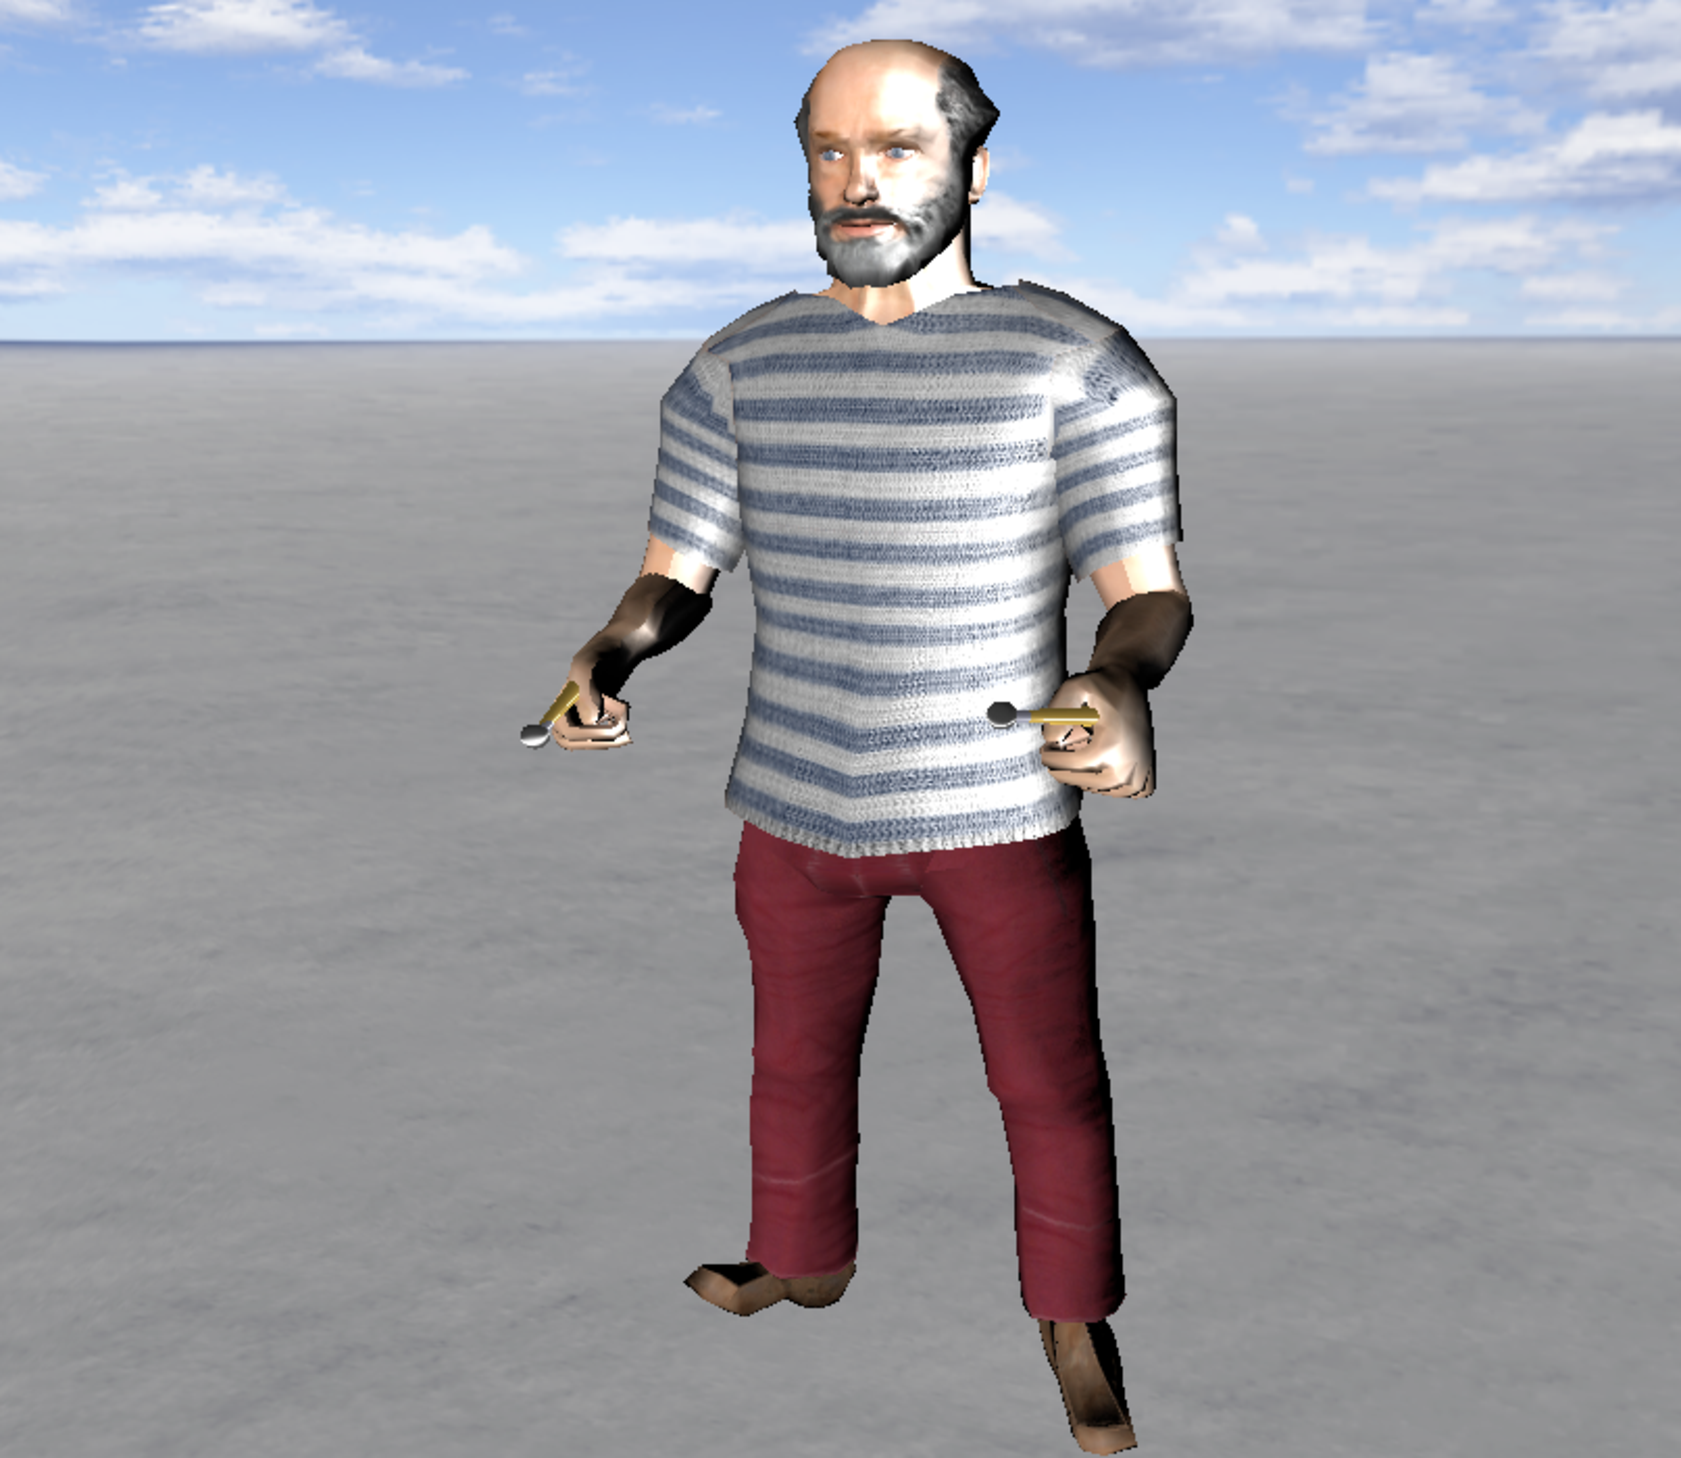
\includegraphics[width=0.48\columnwidth]{Chapters/2/Pics/Pdf/KinDyn1.pdf}}
		\subfigure[]{\label{fig:kinDyn3}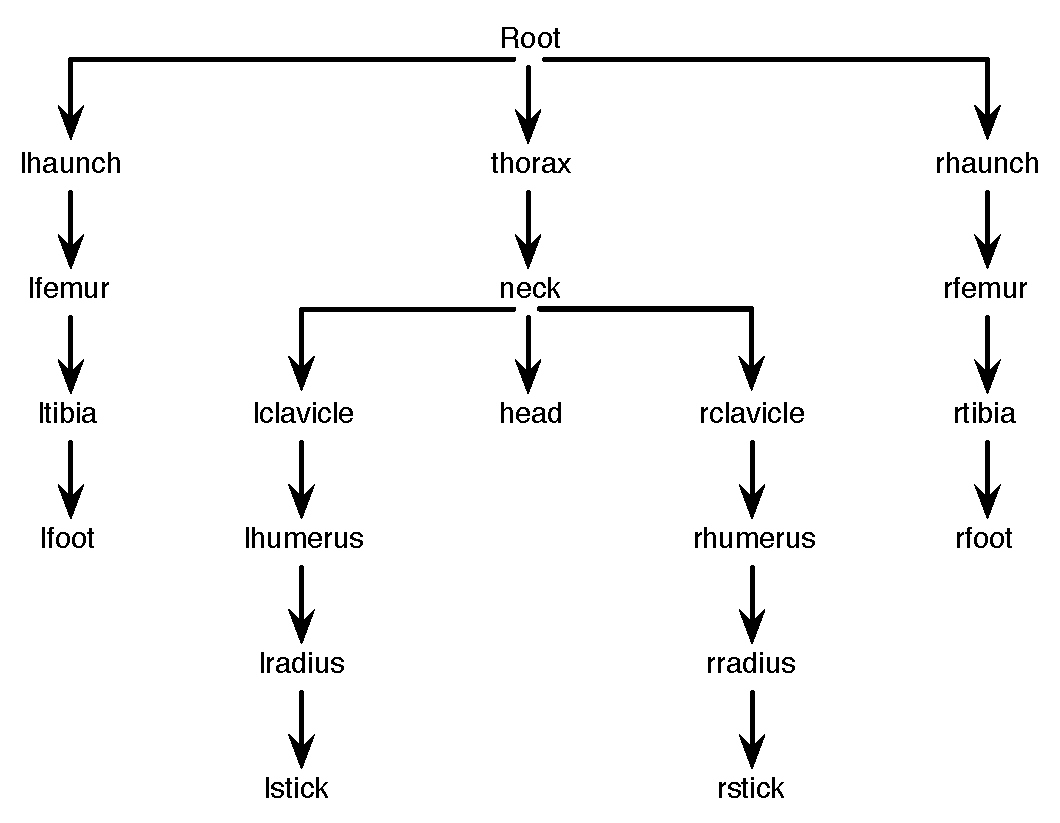
\includegraphics[width=0.48\columnwidth]{Chapters/2/Pics/Pdf/Kin.pdf}}
		\subfigure[]{\label{fig:kinDyn2}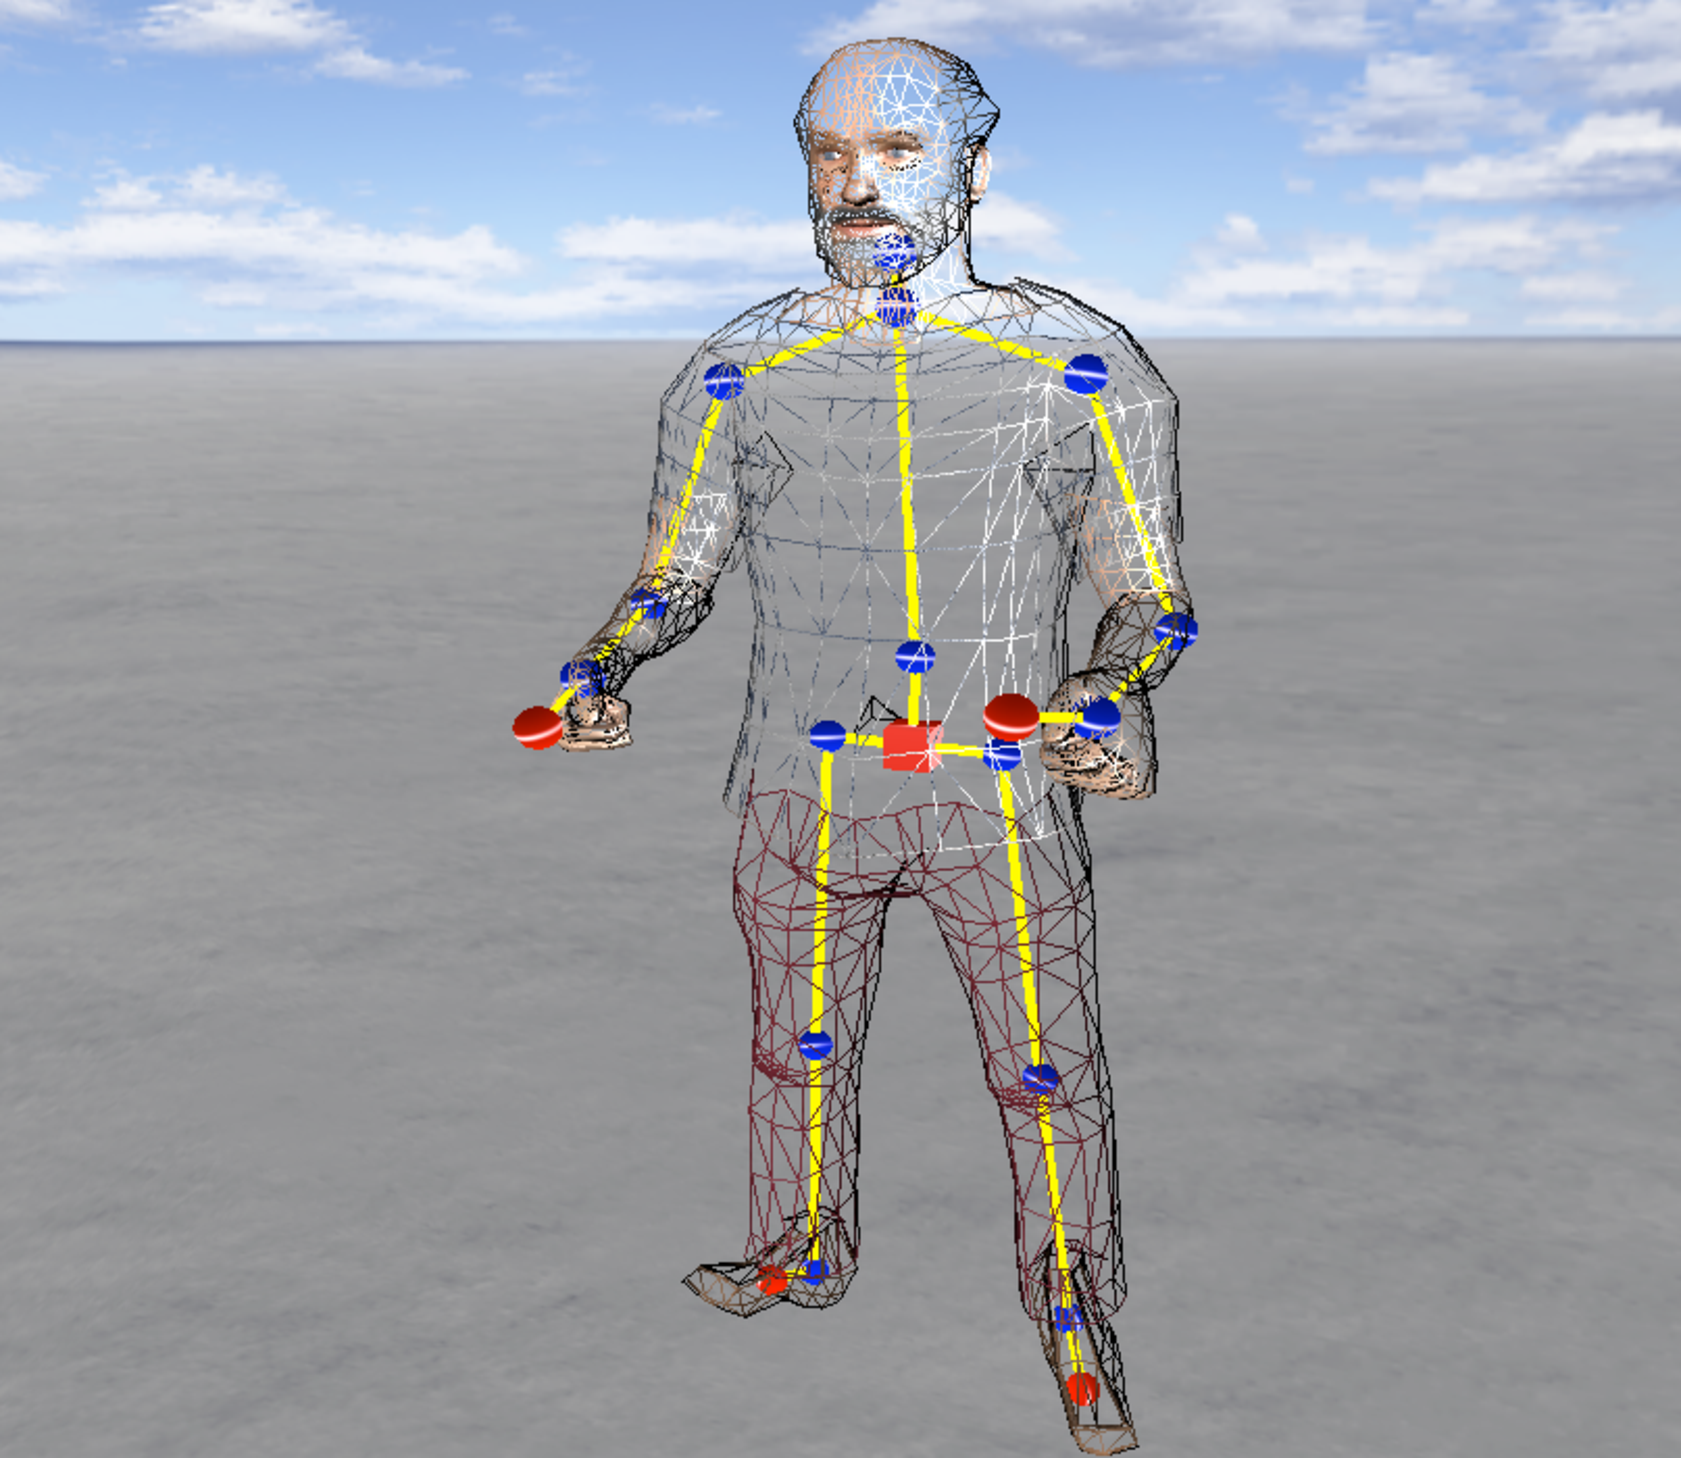
\includegraphics[width=0.48\columnwidth]{Chapters/2/Pics/Pdf/KinDyn2.pdf}}
		\subfigure[]{\label{fig:kinDyn4}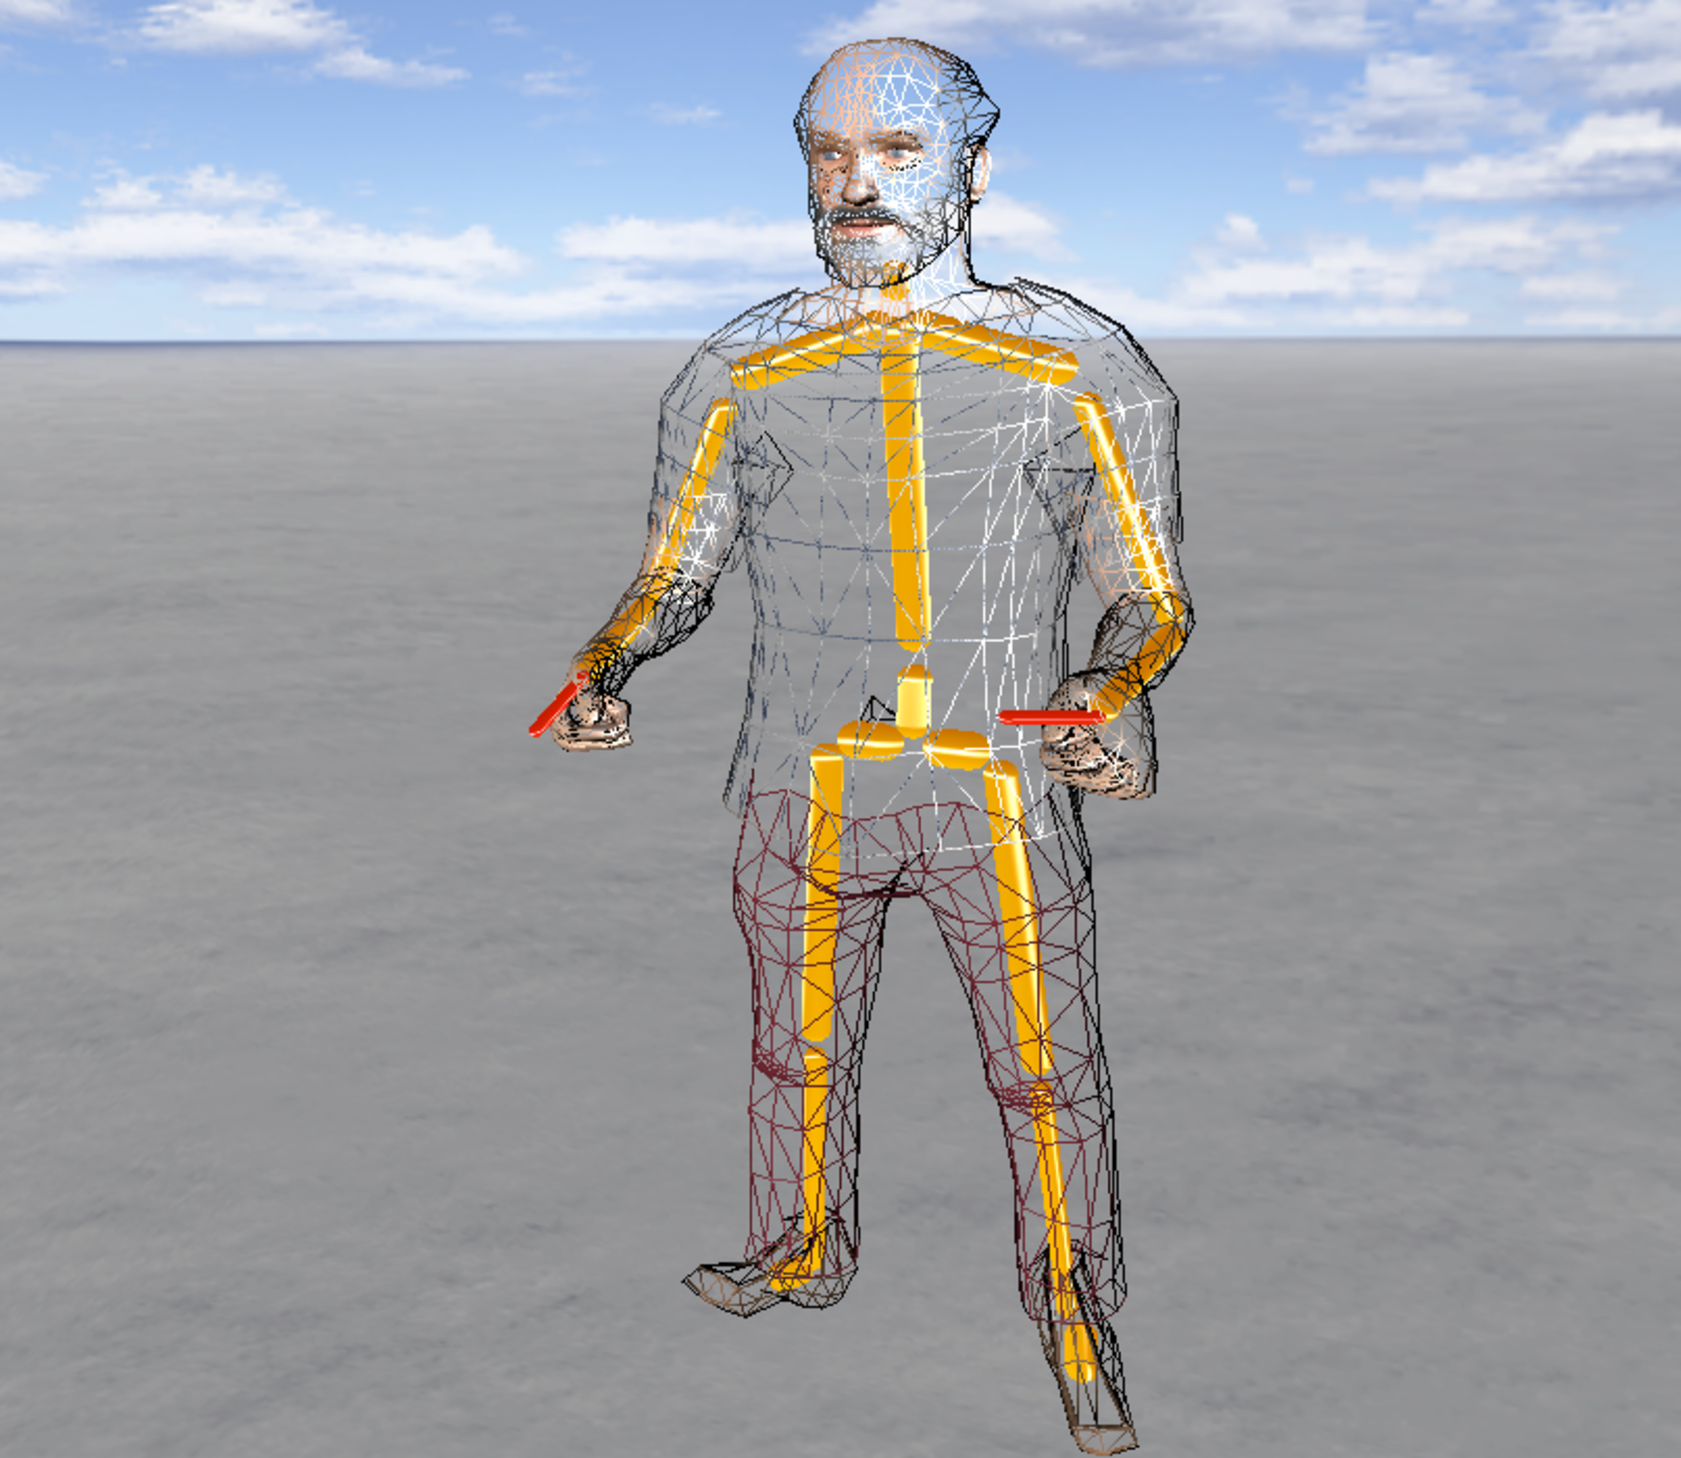
\includegraphics[width=0.48\columnwidth]{Chapters/2/Pics/Pdf/KinDyn4.pdf}}
	\end{center}
	\vspace{-0.5cm}
	\caption[Kinematics and physics representations of a virtual character]{Kinematics and physics representations of a virtual character: (a) final virtual character, (b) the hierachical tree structure, (c) an example of an underlying kinematic representation with its root (red box), set of joints (spheres) and implicit limbs (yellow lines), (d) an example of an underlying physic representation with its explicit limbs (capsule-shaped rigid bodies).}
	\label{fig:kinDynModels}
\end{figure}


			\subsubsection{Kinematics-based Representation}
			\label{subsubsec:CA_VCM_Kinematic}

Virtual characters can be represented by a \emph{kinematic} representation $\boldsymbol{T^K}$, which gives mainly a \emph{geometrical} interpretation of the human anatomy. Such a representation defines implicitly the limbs (or bones) of the virtual human by segments between paired joints. This hiearchical structure is defined by a root joint $\boldsymbol{j^K_r}$ (usually the pelvis) and a set of child joints $\boldsymbol{j^K}$, \myequname \eqref{eq:kinRepresentation}.\\

The kinematic system $\boldsymbol{T^K}$ is then defined by the observation of its state over time, \emph{i.e.} a kinematic configuration (or \emph{pose}) $\boldsymbol{q^K}$. $\boldsymbol{q^K}$ is composed of the root joint position $\boldsymbol{r}$ and the angular state of each child joint $\boldsymbol{\Theta^K}$, \myequname \eqref{eq:kinConfiguration}. The latter may have several \emph{degrees of freedom} (or \emph{DoFs}), thus constraining the motion of the virtual character.

\begin{equation}
	\boldsymbol{T^K} = [\boldsymbol{j^K_r}, \boldsymbol{j^K} = \lbrace j^K_i\rbrace_{i \in [1 \dots n]}]
\label{eq:kinRepresentation}
\eqcaption{Virtual character kinematic representation}
\end{equation}

\vspace{-0.4cm}

\begin{equation}
	\boldsymbol{q^K} = [\textbf{r}, \boldsymbol{\Theta^K} = \lbrace \Theta^K_i\rbrace_{i \in [1 \dots n]}]
\label{eq:kinConfiguration}
\eqcaption{Virtual character kinematic configuration}
\end{equation}

\myfigname \ref{fig:kinDyn2} depicts an example of kinematic representation of a virtual character, with its root position (red box), set of joints (spheres) and implicit limbs (yellow lines). A standard kinematic representation for modeling virtual characters is commonly used for this type of approach \citeCGA{hanim}, easying the comparison, sharing and reusability of representations.


			\subsubsection{Physics-based Representation}
			\label{subsubsec:CA_VCM_Physic}

The \emph{physical} representation $\boldsymbol{T^D}$ of a virtual character provides a \emph{dynamic} interpretation of the human anatomy. In this case, the bones are explicitly modeled by a set of rigid solids $\boldsymbol{s^D}$ articulated by mechanical joints $\boldsymbol{j^D}$, \myequname \eqref{eq:dynRepresentation}. Every solid composing this physical representation $\boldsymbol{s^D}$ is parameterized by physical characteristics such as its mass \emph{m}, density \emph{d} and inertia tensor \emph{I}. Mechanical joints $\boldsymbol{j^D}$ can also be characterized by several DoFs constraining the motion, as well as physical features influencing the relative behavior between solids at the joint level.\\

The observation of the state of $\boldsymbol{T^D}$ over time leads to a dynamic configuration $\boldsymbol{q^D}$, composed of each rigid body linear-angular position $\boldsymbol{r^D}$ as well as each mechanical joint angular position $\boldsymbol{\Theta^D}$, \myequname \eqref{eq:dynConfiguration}. 

\begin{equation}
	\boldsymbol{T^D} = [\boldsymbol{s^D} = \lbrace m^D_i, d^D_i, I^D_i\rbrace_{i \in [1 \dots n]}, \boldsymbol{j^D} = \lbrace k^D_{s, j}, k^D_{d, j}\rbrace_{j \in [1 \dots m]}]
\label{eq:dynRepresentation}
\eqcaption{Virtual character dynamic representation}
\end{equation}

\vspace{-0.4cm}

\begin{equation}
	\boldsymbol{q^D} = [\boldsymbol{r^D} = \lbrace r^D_i, \Theta^D_{r, i}\rbrace_{i \in [1 \dots n]}, \boldsymbol{\Theta^D} = \lbrace \Theta^D_j\rbrace_{j \in [1 \dots m]}]
\label{eq:dynConfiguration}
\eqcaption{Virtual character dynamic configuration}
\end{equation}

\myfigname \ref{fig:kinDyn4} shows an example of a physic representation of a virtual character made of capsule-shaped rigid bodies. These models usually assume a uniform density distribution of the rigid bodies. Human body measures can be considered for initializing the physical properties of the rigid bodies composing such a representation \citeCGA{dempster:AJA67, AIST}.


		\subsection{Motion Control of Virtual Characters}
		\label{subsec:CA_MC}

The characteristics of these different virtual character representations previously presented intrinsically differ from the nature of human motion features they focus on. They differ as well as on the low/high level control properties and environment interactions that they can take into account.\\

The \emph{kinematic} model can be considered as an \emph{effect-centered} representation, offering a well formulated formalism for a high task control level. It however provides no explanation of the causes that are at the origin of the motion system $\boldsymbol{T^S}$, and harldy provides the opportunity to integrate interactions with its surrounding environment. Kinematics-based animation techniques will therefore use methods on the top of the geometrical observation $\boldsymbol{q^K}$ of the human motion, in order to reproduce, adapt or modify this observation (section \ref{subsubsec:CA_MC_Kinematics}).\\

Conversely, the \emph{physical} representation can be considered as a \emph{cause-centered} model since it makes available a responsive model to the application of forces and torques on the system $\boldsymbol{T^D}$. It gives a quite low level control scheme, but facilitates its interaction with the surrounding environment. Physics-based animation techniques aim at building control paradigms to \emph{produce} adequate forces and torques that are the cause of the human motion based on the state observation $\boldsymbol{q^D}$ (section \ref{subsubsec:CA_MC_Physics}).\\

Finally, some contributions aim at taking advantage of each representation's assets, therefore mixing kinematics-based and physics-based animation techniques. We will refer to this kind of formulations as hybrid methods (section \ref{subsubsec:CA_MC_Hybrid}).\\

It should be noted that this state of the art mainly focuses on the various \emph{control} models that have been introduced in the \emph{Computer Animation} community. The recall and derivation of equations is justified as a means of precisely identifying the nature (geometric, kinematic, dynamic) of the parameters that each model refers to.


			\subsubsection{Kinematics-based Methods}
			\label{subsubsec:CA_MC_Kinematics}

The animation of virtual characters has a huge history, which begins with hand-made (cartoon) productions. Two of the most common  kinematics-based computer animation techniques come from this historical background: \emph{keyframing} and \emph{interpolation} (or \emph{inbetweening}). At its initial stage, the process of producing hand-made animations was stamped by its organisational approach (Taylorism), involving firstly senior animators producing action-based drawings (\emph{keyframes}) at targetted specific times of the final animation, and secondly junior animators in charge of linking these \emph{keyframes} by \emph{inbetween} drawings.


				\subsubsubsection{Forward Kinematics}
				\label{subsubsubsec:CA_MC_Kinematics_Fwd}

Inspired by the early works of Walt Disney Studio in the late 1920's, most of \emph{Computer Animation}'s work began therefore with adapting purely traditional 2D techniques to the new possibilities offered by computers \citeCGA{catmull:SIGGRAPH78, lasseter:SIGGRAPH87}. This has led to computer storytelling, keyframe animation (keyframing) \citeCGA{burtnyk:SMPTE71} as well as the elaboration of various interpolation techniques \citeCGA{kochanek:SIGGRAPH84, shoemake:SIGGRAPH85}. Keyframing involves the specification of key postures ($\boldsymbol{q^K}$) so that the virtual character produces the desired task ($\boldsymbol{E^K}$). This process is called \emph{forward kinematics}, \myequname \eqref{eq:kinFormulation}. Then an interpolation technique is used to automatically compute inbetween postures given these keyframes. The interpolation algorithm is of great importance, since it may critically influence the appearance (realism) of the final animation.

\begin{equation}
	\boldsymbol{E^K} = \mathcal{K}(\boldsymbol{q^K})
\label{eq:kinFormulation}
\eqcaption{Forward kinematics formulation}
\end{equation}

While such a process is quite natural for producing animations, it rapidly becomes a tedious and time-consuming task depending on the length of the final animation, and moreover depending on the complexity of the model to put into motion. Particularly in the case of virtual character animation, virtual humans can contain up to sixty DoFs (dimension of $\boldsymbol{\Theta^K}$), making this process chalenging just for instance to place the hand at a desired position. That is the reason why algorithms have been developped for infering the kinematic posture of a virtual character, given only the task to be performed. Such a technique is called \emph{inverse kinematics} (or \emph{IK}).


				\subsubsubsection{Inverse Kinematics}
				\label{subsubsubsec:CA_MC_Kinematics_Inv}

The inverse kinematics problem, \myequname \eqref{eq:invKinFormulation}, provides a formal formulation for automatically computing the kinematics posture $\boldsymbol{q^K}$ of the virtual character given a desired task $\boldsymbol{E^K}$ to accomplish. $\boldsymbol{q^K}$ is typically characterized by all the DoFs defining the virtual character's skeleton, and $\boldsymbol{E^K}$ defines the task, generally the linear and/or augular position of limbs' end-effectors -- such as hands or feet configuration, see red spheres on \myfigname \ref{fig:kinDyn2}.

\begin{equation}
	\boldsymbol{q^K} = \mathcal{K}^{-1}(\boldsymbol{E^K})
\label{eq:invKinFormulation}
\eqcaption{Inverse kinematics formulation}
\end{equation}

The difficulty with this formulation mainly lies in the redundancy of the system $\boldsymbol{T^K}$ which makes the kinematics problem under-determined, as many different kinematics postures $\boldsymbol{q^K}$ can lead to the same desired task $\boldsymbol{E^K}$. More specifically for the human arm, it has been shown that an analytical solution may be determined for an arm model with seven DoFs \citeCGA{korein85}. Additionnal numerical methods can even take into account joint limits \citeCGA{tolani:GM00}.\\

However, when considering controlled systems of higher dimension, an analytical solution to the inverse kinematics problem is not envisageable. In this case, numerical methods are generally deployed, involving either optimization or techniques taking advantage of the availability of motion data.


					\subsubsubsubsection{Optimization Methods}
					\label{subsubsubsubsec:CA_MC_Kinematics_Inv_Jacobian}

Among optimization methods, one of the most widespread solutions to the inverse kinematics problem is to apply a local linearization to \myequname \eqref{eq:kinFormulation} for finding the Jacobian matrix $\mathcal{J}$ of the system to control \citeCGA{whitney:TMMS69}. This process can be seen as relating the effect of small variations in the joint space to small variations in the task space. Jacobian-based inverse kinematics schemes then rely on the inversion of this Jacobian matrix $\mathcal{J}$, \myequname \eqref{eq:jacobInvKinFormulation}. This inversion condition is however not always realized due to the fact that in most of the cases $\mathcal{J}$ is not squared (again due to the redundancy of the system) and possibly singular.

\begin{equation}
	\boldsymbol{\Delta q^K} = \mathcal{J}^{-1}(q^K) . \Delta\boldsymbol{E^K}
\label{eq:jacobInvKinFormulation}
\eqcaption{Jacobian-based inverse kinematics formulation}
\end{equation}

Alternatives to the inversion of $\mathcal{J}$ have consequently been proposed, firstly to solve its invertibility, such as the transpose of the Jacobian matrix $\mathcal{J}^{T}$ \citeCGA{wolovitch:DC84}, its pseudo-inverse $\mathcal{J}^{\dag}$ \citeCGA{greville:SIAM59}, or other methods introducing biological functions to solve this inverse problem \citeCGA{gibet:JAI94}. Secondly, solutions have been proposed to cope with its singularity \citeCGA{wampler:SMC86}, leading to an adaptation of the pseudo-inverse $\mathcal{J}^{\dag}_{\lambda}$ parameterised by a damping factor ($\lambda$) that can be automatically and dynamically computed \citeCGA{maciejewski:JRS88}.

\begin{equation}
	\boldsymbol{\Delta q^K} = \mathcal{J}^{\dag}_{\lambda}(q^K) . \Delta\boldsymbol{E^K} + (I - \mathcal{J}^{\dag} . \mathcal{J}) . \Delta \boldsymbol{z^K}
\label{eq:jacob2InvKinFormulation}
\eqcaption{Jacobian-based inverse kinematics formulation, secondary tasks}
\end{equation}

Other solutions propose the combination of such alternatives while exploiting the redundancy of $\boldsymbol{T^K}$ by defining secondary tasks ($\Delta \boldsymbol{z^K}$) to be performed. This has been firstly done in \citeCGA{liegeois:SMC77}, by expressing these seconday tasks on the null space of $\mathcal{J}$, \myequname \eqref{eq:jacob2InvKinFormulation}.

It has the advantage of allowing the integration and respect of high-level control taks such as object avoidance \citeCGA{siciliano:ICAR91}, prioritized physical and shape constraints \citeCGA{baerlocher:IROS98, baerlocher:VC04, leCallenec:GM06} as well as ergonomic constraints \citeCGA{yang:SMPT05}.\\


%					\subsubsubsubsection{Other Optimization Methods}
%					\label{subsubsubsubsec:CA_MC_Kinematics_Other}
%					\noindent{\textbf{\small{Other Optimization Methods}}}\\

Fundamentally different iterative approaches avoid the Jacobian matrix inversion, such as the Cyclic-Coordinate-Descent (CCD) method \citeCGA{wang:IEERA91}. It is an heuristic formulation of the inverse kinematics problem, that can be compared to the linearization of \myequname \eqref{eq:kinFormulation}. More recently a hierachical CCD algorithm involving the independent treatment of joint sub-groups as well as task priorities has been proposed \citeCGA{kulpa:Humanoids05}. %Such optimization formulations explicits the inversion problem as an optimization problem, typically by minimizing a cost function under a set of constraints \citeCGA{gill81}.

%\begin{equation}
%	Minimize\ \boldsymbol{E_{err}} = [\mathcal{K}(\boldsymbol{q^K})-\boldsymbol{E^K}]^T . [\mathcal{K}(\boldsymbol{q^K})-\boldsymbol{E^K}]\ under\ \boldsymbol{C}
%\label{eq:optimization}
%\eqcaption{Optimization-based inverse kinematics formulation}
%\end{equation}

%The effectiveness of such formulation depends highly on the nature of the cost function E, which can range from a simple norm function between the current end-efector state and target to more complex functions. The set of constrains can for example limit the allowed angular motion of joints by the specification of lower and upper bounds. A good introduction to optimization-based numerical methods can be found in \citeCGA{gill81}.\\

%The CCD formulation \citeCGA{wang:IEERA91} differs from other optmization methods by treating sequentially each joint (from the most distal to the base) composing the kinematic representation of the virtual character. It is an heuristic formulation of the inverse kinematics problem, that can be compared to the linearization of \myequname \eqref{eq:kinFormulation}, since it treats independently each joint of the controlled kinematic structure. More recently a hierachical CCD algorithm involving the independent treatment of joint sub-groups as well as task priorities has been proposed \citeCGA{kulpa:Humanoids05}.\\


					\subsubsubsubsection{Example-based Methods}
					\label{subsubsubsubsec:CA_MC_Kinematics_Task}

Kinematics-based animation techniques are widely used both in the \emph{Computer Animation} research community and in the industrial domain. One open question is how to specify the task to be accomplished by the virtual character, whatever a \emph{forward} or \emph{inverse} kinematics scheme is used. Methods then consist in synthesizing new movement sequences from the capture of examples of human motion. This includes the combination of \emph{IK} formulations with motion data, learning approaches, as well as methods for retrieving, adapting, combining and retargetting existing motion data.\\


						\noindent{\textbf{\small{Motion capture solutions}}}\\

A growing demand in human motion data has rised these past few years in industrial fields such as computer games and 3D animation films. This has led to the conception of various hardware for reliably capturing human motion. It includes mainly two classes of hardware: intrusive and non-intrusive systems.

\begin{figure}%[H]
	\begin{center}
		\subfigure[]{\label{fig:mocap1}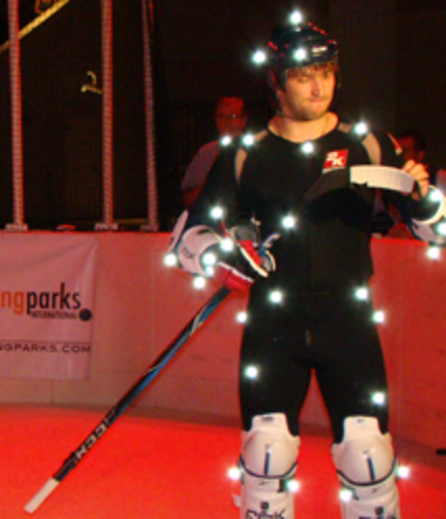
\includegraphics[height=37mm]{Chapters/2/Pics/Pdf/vicon.pdf}}
		\subfigure[]{\label{fig:mocap2}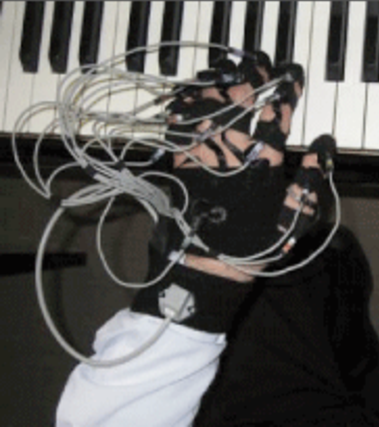
\includegraphics[height=37mm]{Chapters/2/Pics/Pdf/liberty.pdf}}
		\subfigure[]{\label{fig:mocap3}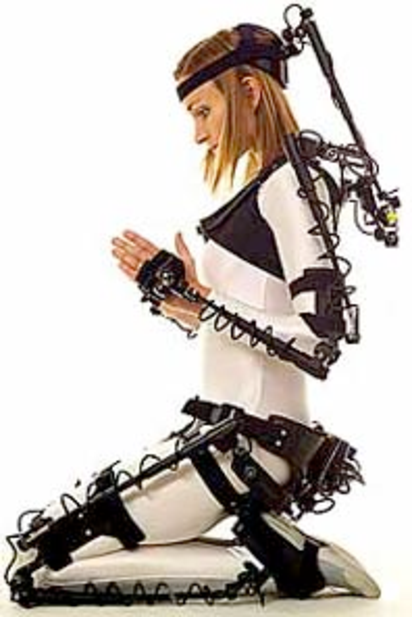
\includegraphics[height=37mm]{Chapters/2/Pics/Pdf/metamotion.pdf}}
		\subfigure[]{\label{fig:mocap4}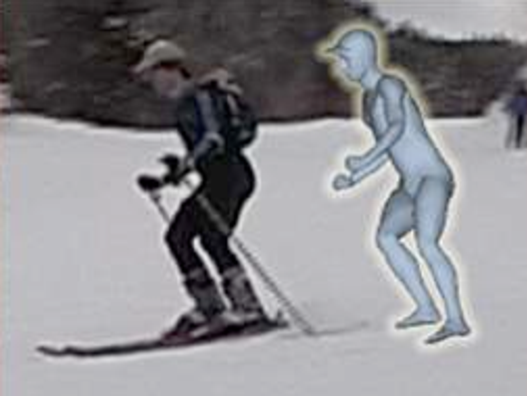
\includegraphics[height=37mm]{Chapters/2/Pics/Pdf/videomocap.pdf}}
	\end{center}
	\vspace{-0.5cm}
	\caption[Motion capture systems]{Motion capture systems, from left to right: (a) infrared camera tracking (courtesy of \citeCGA{vicon}), (b) electromagnetic tracking (courtesy of \citeCGA{polhemus, mitobe:SIGGRAPH06}), (c) electromechanical sensors (courtesy of \citeCGA{metaMotion}) and (d) video-based tracking (courtesy of \citeCGA{vlasic:TOG07}).}
	\label{fig:kinMoCap}
\end{figure}

Among intrusive methods, optical systems involve reflective markers put on real humans whose motion can be triangulated by infrared cameras, such as Vicon hardware \citeCGA{vicon}. The motion of electromagnetic sensors can also be measured relatively to a magnetic reference, such as Polhemus solutions \citeCGA{polhemus}. Another intrusive method is provided by electromechanical systems which are based on exoskeletons, such as systems provided by Meta Motion \citeCGA{metaMotion}. As shown in \myfigname \ref{fig:kinMoCap}, such hardware solutions can be quite intrusive and therefore possibly constraint the motion that is to be recorded.

On the contrary, non-intrusive methods do not rely on sensors directly in contact with captured human, and involve usually video-based processing methods, \myfigname \ref{fig:mocap4}. Such techniques appear to be a promising approach for capturing the human motion in many capture condition \citeCGA{vlasic:TOG07, qualisys}, in both indoor and outdoor environments.\\


						\noindent{\textbf{\small{Motion-driven Inverse Kinematics}}}\\

Early works among motion-driven inverse kinematics contributions aimed at infering a kinematic posture target for achieving a desired task, while preserving the characteristics (synergies, styles) of a given motion.

It has been first proposed to interpolate between available motion clips that are similar in the kinematic posture space to a posture that show the desired task \citeCGA{wiley:IEEE-TMMS97}. The cost reduction of such an approach due to the required amount of motion clips has been addressed in \citeCGA{rose:CGF01}. \citeCGA{komura:CGI03} then proposed a formulation for computing a weight matrix representing the style of a single motion example at the joint level. Such weight matrix combined with an \emph{IK} process allows to synthesize new movements while preserving the style of the original motion.

%Single motion as input: \citeCGA{tak:CGIM00} solving IK to respect end-effector targets as well as imitating an input motion. then \citeCGA{komura:CGI03} analogously provides a way of solving the IK formulation while retaining inertia and mass body features that characterize the style of a given motion as input.\\

Data reduction techniques have also been considered for representing motions in latent spaces. This generally involves the use of the Principal Component Analysis (\emph{PCA}) \citeCGA{alexa:CGF00}. It has then been shown that the respect of constraints in such PCA space combined with a prioritized \emph{IK} formulation can lead to the synthesis of new motions \citeCGA{carvalho:CAVW07}. Other solutions have been proposed for taking advantage of such latent spaces, for instance for modeling time-varying joint synergies by linear functions \citeCGA{raunhardt:VC09}.\\ % as well as motion compression in the quaternionic sapce \citeCGA{tournier:CGF09}.\\


						\noindent{\textbf{\small{Learning Methods}}}\\

The basic approach of learning methods consists in learning the mapping between kinematic configurations and end-effector tasks.

Hidden markov nodels \citeCGA{brand:SIGGRAPH00} as well as linear dynamic systems \citeCGA{li:SIGGRAPH02} have been used for learning the style of human motion examples. Models based on radial basis functions \citeCGA{rose:CGF01} and Gaussian latent variables \citeCGA{grochow:TOG04} have also been used for learning kinematic configurations with the aim of solving the inverse kinematics problem. This problem has been solved by the determination of the Jacobian inverse matrix through the learning of local transformations \citeCGA{gibet:CASA03}. The mapping between poses and style parameters can also been learnt by using Gaussian mixture models \citeCGA{wang:CAVW06}. Physical constraints can be learnt from existing motion by clustering \citeCGA{liu:TOG05}, and user-defined constraints can be taken into account by combining these latter with a statistical model learnt from motion capture data \citeCGA{chai:TOG07}. Another solution is to use Monte Carlo casting alongside with a sequential particular filtering formulation \citeCGA{courty:AMDO08}. Finally, another approach is presented in \citeCGA{aubry:GW09} to model joint synergies from existing movement sequences for solving the \emph{IK} problem.\\


%					\subsubsubsubsection{Motion Data-based Methods}
%					\label{subsubsubsubsec:CA_MC_Kinematics_Task_MoCap}

						\noindent{\textbf{\small{Motion Retrieval, Combination and Retargetting}}}\\

The ever growing availability of human motion data \citeCGA{cmumocap} has led to new research questions. Although such research directions are out of the scope of this thesis, we give some hints on research trends in extending the possibilities of motion capture databases, such as motion retrieval, motion combination and motion retargetting to cite a few.\\

Motion capture databases usually collect thousands of motion clips, creating challenges to store, access and process the data present in the database. Motion retrieval techniques usually work on two sub-problems. On the one hand it involves the identification of an adequate representation (indexing) of motion data so that high-dimension motion clips can be characterized in a low-dimension space. Secondly, reliable similarity measures have to be determined so that the comparison (retrieval) of motion chunks can be possible. %firstly finding a well-suited dimension reduction leading to a feature-based characterization of the database, secondly determining a distance metric for comparing motion chunks on this feature space.

%Early works defined dimension reduction methods such as spectral transformations \citeCGA{agrawal:FDOA93}, clustering \citeCGA{liu:CVIU03} or Principal Component Analysis (PCA) \citeCGA{forbes:SCA05}. Hand-made annotations \citeCGA{arikan:TOG03} and semantic informations \citeCGA{awad:IVA09} have also been used for reducing the dimention of motion capture databases. As for distance metrics, recent work on Dynamic Time Warping \citeCGA{kovar:SCA03} or Uniform Scaling \citeCGA{keogh:VLDB04} have yielded to reliable solutions, even if the numerical nature of the distances keep away for the moment from the desired semantic level of queries.\\

Regarding motion representations, geometric features have been proposed describing the dependencies between joints motion clips \citeCGA{muller:TOG05, lin:GRAPHITE06}. Another representation is to involve more or less automatic methods for indexing motion clips with annotations \citeCGA{arikan:TOG03, barbic:GI04, awad:IVA09}, thus characterizing differences in the semantic nature of a motion database. Other reduction methods represent motion in low-dimension spaces. Such techniques use for instance spectral transformations \citeCGA{agrawal:FDOA93}, linear reductions methods such as PCA \citeCGA{forbes:SCA05} or non-linear ones such as Isomap \citeCGA{xiang:IIHMSP07}. Clustering can also be involved in such data reduction methods \citeCGA{liu:CVIU03}.

Among simple similarity measures, works have involved measures that cope with velocity and acceleration differences, and suggest to use rotation-invariant metrics on motion clips of the same length \citeCGA{kovar:TOG02}. Another method is Dynamic Time Warping (\emph{DTW}) which gives generally good results \citeCGA{ding:VLDB08} for finding an optimal alignment between motions. Aligning two motion sequences of different time lengths in DTW has been proposed in \citeCGA{keogh:VLDB04}.\\

Highly related to motion retrieval are motion combination techniques, which aim at creating new animations from an available set of motion chunks. Multivariate interpolation has been introduced \citeCGA{rose:IEEECGA98} through a verb (motion) /adverb (interpolation) metaphor. It typically uses a verb graph linking therefore motion clips with each other, in which allowed transitions can also be computed automatically \citeCGA{kovar:SCA03}. Other techniques use motion graphs for modeling envisageable transitions between motion clips \citeCGA{kovar:TOG02}, in which annotations \citeCGA{arikan:TOG03} and path planning \citeCGA{mahmudi:I3D08} can be integrated.\\ %A linear interpolation in the PCA space has also been shown to be effective for combining new bipedal motions \citeCGA{glardon:CASA04}. 

Motion retargetting deals with the problem of adapting a given motion to other conditions or styles. Retargetting has been involved for adapting motion to different skeleton sizes \citeCGA{gleicher:SIGGRAPH98} as well as kinematic constraints \citeCGA{bruderlin:SIGGRAPH95}. Concerning style transformation, it has been observed that various frequency filtering bands can produce stylistic conditions. Emotional transformations between motion data have first been proposed in \citeCGA{amaya:GI96} based on signal processing methods. Latter works have for instance combined style translations with inverse kinematics \citeCGA{grochow:TOG04} and time warping \citeCGA{hsu:TOG05, heloir:CAVW06}.


%					\noindent{\textbf{\small{Conclusion}}}\\

%Motion data-based methods achieve a high realism in the resulting animations. However, this is mainly due to the inherent realism of captured motion. Apart from the motion-driven inverse kinematics methods detailed previously, there is for the moment no other solution in this avenue apart from capturing all possible human gestures to build an extensive motion capture database that could be used for creating any animation sequence.\\


%					\subsubsubsubsection{Task Modeling}
%					\label{subsubsubsubsec:CA_MC_Kinematics_Task_Know}

%Most of the time, motion data-based techniques still need a motion editing step which relies highly on the animator's talent depending on the desired artistic effect to accomplish. As proposed in the \emph{Biomechanics} and \emph{Neuroscience} research fields, an alternative is to consider a fine analysis of human motion, specifically by studying motion production laws that are at the origin of human motion. For a complete review of these invariant motion laws, readers are refered to \citeCGA{gibet:HdR02, hale:PhD03}.\\

%Due to the somewhat controversial statement underlying the existence of these motion laws, its use in the modeling of the motion to be animated is quite sporadic. Such invariant motion laws have nevertheless been used explicitly as motion generation laws in computer animation systems in \citeCGA{zeltzer:IEEECGA82, kopp:CA02}. Moreover, some of these motion invariants have also been invoked as quantitative criteria for evaluating the naturalness of synthesized motions \citeCGA{mataric:AAMAS99, gibet:JVLC01, kopp:CAVW04}.\\

%Many theories have been proposed to explain the mechanisms of the \emph{CNS}, a complete overview of these theories will however not be addressed in details in this bibliographic work since it would need a complete review of the Motor Control theory. Interested readers are refered to \citeCGA{hale:PhD03} for a comprehensive review. Traditionnaly, two concurrent models explain motor control tasks in Neuroscience: General Motor Programs (\emph{GMPs}) and the \emph{Equilibrium Point Control} theory. Here we will focus on \emph{GMPs} as the \emph{Equilibrium Point Control} is treated elsewhere (subsection \ref{subsubsubsubsec:CA_MC_Physics_Controllers}).\\

%\emph{GMPs} have been first introduced \citeCGA{schmidt:PR75} as a generalization of \emph{Motor Programs} \citeCGA{keel:PB68}, namely for taking into account sensory feedback that is necessary for the elaboration of spatio-temporal motor commands to produce an action. \emph{GMPs} state the existence of learning processes for assigning differently parameterized motor programs to various motion classes. This is supported by the observation of invariant laws in human motion \citeCGA{gibet:GW04}, such as:

%\begin{itemize}

%	\item the \emph{Fitt}'s law \citeCGA{woodworth:PR1899, fitts:JEP54}, which relates the movement duration to the task distance and difficulty

%	\item the \emph{isochrony} law \citeCGA{freeman:PR14}, relating the movement duration to its amplitude which was formerly observed in \citeCGA{binet:RP1893}

%	\item the \emph{two-third power} law \citeCGA{viviani:N82}, which relates the movement angular velocity to its trajectory curvature

%	\item the \emph{minimum jerk} \citeCGA{flash:N85}, stating an underlying motor command law that optimizes the smoothness of performed movements, its relation to the \emph{two-third power} law has been shown in \citeCGA{wann:JEP88}

%\end{itemize}

%Animation systems taking advantage of such human motion invariants are nevertheless quite rare, mainly because of their lack of generality since their vast majority have been demonstrated for pointing gestures. The scalability of motion invariants to other gesture types has not been demonstrated, so that elaborating control systems upon them would necessitate a fine and accurate analysis preprocess.\\


				\subsubsubsection{Conclusion}
				\label{subsubsubsec:CA_MC_Kinematics_Conclusion}

Kinematics-based animation techniques are shown to be well-suited methods when a high-level control over the task specification is needed. They give a formal framework for managing several tasks at the same time (such as secondary goals with Jacobian-based techniques) or for combining motion chunks (motion combination and retargetting).

As for inverse kinematics methods, an extensive evaluation of some of the previously cited techniques can be found in \citeCGA{unzueta:GM08}. It shows namely that neither the Jacobian transpose nor CCD formulations give satisfactory results in terms of motion quality, compared to other Jacobian-based methods.

Concerning learning techniques, one critical issue is that new motion are generally obtained by interpolating the learnt parameters, while no guaranty is provided to ensure that the resulting new movement sequences still respect the physical laws of motion.

In addition, the main drawback of methods dealing with motion retrieval and combination is that there is for the moment no other solution in this avenue apart from capturing all possible human gestures to build an extensive motion capture database that could be used for creating any animation sequence.

Despite the high realism in the resulting animations obtained by the previoulsy detailed methods, their main drawback lies in the fact that they do not deal with dynamics. Therefore, they cannot take into account the possible physical interactions of virtual characters with their environment. It is true both for simply modeling physical interactions (for instance the gravitation field or collisions) as well as reusing motion capture in different contexts (even if some hybrid methods are available, see section \ref{subsubsec:CA_MC_Hybrid}).\\

An alternative to this problem is to take advantage of the physical representation of the virtual character, so that environmental interactions can be explicitly modelled.


			\subsubsection{Physics-based Methods}
			\label{subsubsec:CA_MC_Physics}

Animation techniques based on the physical representation of virtual humans are attractive since the synthesized motion implicitly respects the physical motion laws. The virtual character is put into motion by the application of forces ($\boldsymbol{F^D}$) and torques ($\boldsymbol{\tau^D}$) so that the physical representation reaches a desired configuration $\boldsymbol{q^D}$. This scheme is called the \emph{forward dynamics} formulation, \myequname \eqref{eq:physFormulation}.

\begin{equation}
	\boldsymbol{q^D} = \mathcal{D}(\boldsymbol{F^D, \tau^D})
\label{eq:physFormulation}
\eqcaption{Forward dynamics formulation}
\end{equation}

Although there are several formulations of the motion laws (see the Lagrangian method for example \citeCGA{baraff:SIGGRAPH96, nocent:PhD01}), they are strictly equivalent to Newton's motion laws, which relate the application of forces and torques, \myequname \eqref{eq:physNewtonFormulation},  to the linear ($\boldsymbol{\Gamma}$) and angular ($\boldsymbol{\Omega}$) state of a solid characterized by a mass \emph{m} and an inertia tensor \emph{I}.

\begin{equation}
	\begin{array}{l}
		\boldsymbol{F} = m . \boldsymbol{\Gamma} \\
		\boldsymbol{\tau} = I . \boldsymbol{\dot{\Omega}} + \boldsymbol{\Omega}.I.\boldsymbol{\Omega}
	\end{array}
\label{eq:physNewtonFormulation}
\eqcaption{Newton motion laws}
\end{equation}


				\subsubsubsection{Forward Dynamics}
				\label{subsubsubsec:CA_MC_Physics_Fwd}
				
Forward dynamics implies the explicit application of time-varying forces and torques to any solid composing the physical representation $\boldsymbol{T^D}$ of the virtual character. The update of the physical configuration $\boldsymbol{q^D}$ uses an integration of solids' linear acceleration and angular velocity over time. Such a framework therefore automatically handles external influences, such as the gravitation field as well as the collisions between solids. A comprehensive study of forward dynamics basics can be found in \citeCGA{wilhelms91}.\\

The extention from the simulation of simple objects to fully articulated skeletons is far from straighforward. Early works involved the simulation of motion laws with numerical methods of high complexity. For example, the contribution from \citeCGA{wilhelms:GI85} proposed a solution with a $O(n^3)$ complexity for an articulated chain composed of \emph{n} DoFs. A recursive formulation associated to a tree structure for representing articulated bodies has then been proposed for treating such problem with a complexity reduction to $O(n)$ \citeCGA{armstrong:VC85}.\\

These early works involved the motion simulation of rigid bodies by the independent specification of forces at the joint level, which is admitted to be far too simple, since it does not take into account the integration and simulation of the internal interactions between connected bodies \citeCGA{wihelms:GI86}. Classically, an alternative is to add springed-damped effects (or equivalent) to joints for circumventing this difficulty (see section \ref{subsubsubsubsec:CA_MC_Physics_Controllers}), even if additionnal numerical instabilities then have to be counteracted \citeCGA{girard91}.\\

Despite the availability of accurate mechanical studies of human motion, such as human locomotion \citeCGA{cavagna:JP76, mcmahon:IJRR84}, these contributions generally cannot be straightfowardly integrated into simulation frameworks. Analogously to forward kinematics, the main critical issue of forward dynamics is once again to rely on the animator's intuition for finding the adequate forces and torques to put the physical model into motion.


				\subsubsubsection{Inverse Dynamics}
				\label{subsubsubsec:CA_MC_Physics_Inv}
				
An alternative is to consider the inverse of the forward dynamics formulation, the so-called \emph{inverse dynamics} (or \emph{ID}) problem. It aims at automatically computing the needed forces and torques ($\boldsymbol{F^D}$, $\boldsymbol{\tau^D}$) to be applied on rigid bodies or mechanical joints composing the physical model, so that it reaches the desired configuration $\boldsymbol{q^D}$, \myequname \eqref{eq:invPhysFormulation}.

\begin{equation}
	(\boldsymbol{F^D, \tau^D}) = \mathcal{D}^{-1}(\boldsymbol{q^D})
\label{eq:invPhysFormulation}
\eqcaption{Inverse dynamics formulation}
\end{equation}

Once the dynamic forces and torques are computed, a forward dynamics scheme is nevertheless used to put the physical model into motion. Classically, inverse dynamics methods are highly inspired from robotics, and imply either the respect of constraints along the simulation of motion laws, or the design of specific controllers. At the human body level, controllers can be considered as an \emph{internal} representation of the muscle activity that occurs between the rigid bodies composing the virtual character. Whereas constraint-based methods can be qualified as an \emph{external} formulation since they classically involve a global optimization scheme where no muscle model is provided.


				\subsubsubsubsection{Constraint-based Methods}
				\label{subsubsubsubsec:CA_MC_Physics_Constraints}

Early works have focused on the respect of geometric or kinematic constraints for finding the forces and torques to apply on articulated rigid bodies. Geometrical constraints (for example, a point belonging to an object fixed to a curve or to another object) are typically expressed linearly depending on forces and torques to be found \citeCGA{barzel:SIGGRAPH88}. It leads to the minimization of constraint equations over time. The translation and integration of these geometrical constraints into the minimization system can however conduct to an over-determined system that is difficult to solve. Another solution \citeCGA{isaacs:SIGGRAPH87, arnaldi:PhD88, dumont90} is to compute the forces and torques given a set of kinematic constraints (such as desired linear and angular displacements) that are inserted into a formulation based on the Virtual Works principle of d'Alembert. Among these early works, one of the most complete integrations of kinematics constraints into physical simulation is certainly the work presented in \citeCGA{witkin:SIGGRAPH88}. It is based on the Lagrangian formulation of physics motion laws, in which initial geometrical and physical inputs are given. It then automatically computes the required forces to respect the initial kinematic constraints, and translates the system as a minimization problem. Such an optimization problem often considers the minimization of an energy function depending on the torques $\boldsymbol{\tau^D}$.\\

Most of contributions have then focused on such optimization process, and specifically on its two main drawbacks: the control offered to users, and the computational cost of this approach. 

Concerning the first drawback, enhancing the user control has first been addressed in \citeCGA{cohen:SIGGRAPH92}, giving the possibility to the user to interact with the iterative optimizations so that the convergence to an acceptable solution can be controlled. Users can also focus on time intervals, giving a subtle control over the overall simulation. The optimization process can also be controlled if desired transitions are required \citeCGA{rose:SIGGRAPH96}. Further researchers have addressed the question of defining multi-objective functions that can cope with task priorities in the optimization process \citeCGA{abe:SCA07, jain:TOG09}.

Reducing the computational cost of such optimization-based methods has parallely been addressed, mainly by considering low-dimensional representations of virtual characters \citeCGA{popovic:SIGGRAPH00}, the motion itself \citeCGA{safonova:TOG04} or the underlying motion equations \citeCGA{barbic:TOG08}. Simplified physical constraints also make possible the preservation of dynamic effects to a reduced cost, for example through the enforcement of momentum patterns \citeCGA{liu:SIGGRAPH02}. Cost functions that can be optimized in linear time have also been under study \citeCGA{fang:TOG03} for decreasing this computational cost, highlighting a wide range of possible physical constraints such as bar and ground contact as well as flight phases.\\

Despite all these efforts, optimization-based methods are admitted to still have a high computational cost that moves away from real-time. The improvements detailed above for lowering the computational cost of such methods can also have an impact on the physical realism of the result, as attested in \citeCGA{vanWelbergen:EG09}.


				\subsubsubsubsection{Controller-based Methods}
				\label{subsubsubsubsec:CA_MC_Physics_Controllers}

Contrary to constraint-based methods, controller-based methods do explicitly model the muscle activity between the rigid bodies composing the virtual character. We can therefore consider such controllers as an integral part of the dynamic model of the virtual character. Such contributions are motivated by early works on the the Hill-type muscle model \citeCGA{zajac90}, whose spring-like effect is considered to be a key component of human postural stability:\\

" It turns out that for stable equilibrium the neuro-musculoskeletal system must possess the attributes of springs, and that for stability, these springs must exceed a certain critical stiffness. The passive, relaxed person is inherently instable at many levels. (...) Certainly the central nervous system is partly responsible for this behaviour, but the primary mode of its influence can be considered to be adjusting muscle 'spring-like' behaviour. " \citeCGA{andersson90}.\\ %p.\ 384

An explicit modeling of the Hill muscle model has been presented in \citeCGA{lee:TOG06} for a complete simulation of neck dynamics, however such an option is currently banned for real-time animation since it necessitates a highly time-consuming preprocess (neural networks) for training the controller.\\

Most of works on controller-based methods have therefore focused on simplified formulations of the Hill muscle. It has led to the design of controllers for specific motor tasks, involving for instance two types of spring-like muscle models: the Proportional-Derivative (\emph{PD}) and the Agonist-Antagonist (\emph{AA}) formulations. Researchers have also tackled the issues of automatically adapting, tuning as well as composing such controllers.\\


					\noindent{\textbf{\small{Proportional-Derivative Control}}}\\

Precursor works have studied the design and adaptation of robotics-inspired controllers to the control of virtual characters \citeCGA{raibert86, raibert:SIGGRAPH91}. In recent years, most of contributions have focused on formulating motor commands applied to each mechanical joint in terms of proportional-derivative controllers. For each joint's degree of freedom, a PD controller is attached to paired rigid bodies whose relative motion is constrained by a springed-damped effect.\\

A PD controller is therefore traditionnally composed of two terms, a proportional term parameterized by a stiffness coefficient $k_s$ and a derivative term parameterized by a damping coefficient $k_d$. The proportional term models the muscle tension effect whereas the derivative term acts as the muscle relaxation. Given the angular state of the mechanical joint ($\boldsymbol{\Theta^D}$, $\boldsymbol{\dot{\Theta^D}}$), and given a desired (target) joint configuration ($\boldsymbol{\Theta^D_t}$, $\boldsymbol{\dot{\Theta}^D_t}$), a control torque $\boldsymbol{\tau^D}$ is computed so that its application on the linked rigid bodies put them into motion towards the desired configuration, \myequname \eqref{eq:invPhysPDFormulation}.

\begin{equation}
	\boldsymbol{\tau^D} = k_s . (\boldsymbol{\Theta^D_t} - \boldsymbol{\Theta^D}) + k_d . (\boldsymbol{\dot{\Theta}^D_t} - \boldsymbol{\dot{\Theta}^D})
\label{eq:invPhysPDFormulation}
\eqcaption{\emph{PD} control formulation}
\end{equation}

A substantial amount of contributions have focused on the design of PD controllers for specific motor tasks. It includes the PD control of walking, jumping \citeCGA{hodgins:ICRA91}, stairs climbing \citeCGA{hodgins:TRA91}, as well as running, cycling, vaulting and balancing \citeCGA{hodgins:SIGGRAPH95}. PD control has also been used for simulating boxing fights \citeCGA{zordan:SCA02}, swimming motion \citeCGA{yang:SCA04}, as well as breast motion \citeCGA{zordan:SCA04, dilorenzo:TOG08}.\\

Usually, torques computed by the PD control formulation are applied with respect to the relative frame formed between the linked rigid bodies. Is has been shown however that expressing and applying the torques $\boldsymbol{\tau^D}$ towards the world frame leads to a better simulation stability \citeCGA{wrotek:SIGRAPH06}.\\


					\noindent{\textbf{\small{Agonist-Antagonist Control}}\\

Contrary to the PD controller with its unique spring model, the Agonist-Antagonist control formulation integrates two spring-like behaviors that are intended to model the spring-like behavior of two opposite agonist-antagonist muscles. \emph{AA} control is therefore composed of two tension proportional terms (parameterized by the coefficients ${k_s}_L$ and ${k_s}_H$) and a relaxation derivative term (parameterized by the damping coefficient $k_d$). Note that this formulation only needs the angular joint limits ($\boldsymbol{\Theta^D_L}$, $\boldsymbol{\Theta^D_H}$) and its current angular state ($\boldsymbol{\Theta^D}$, $\boldsymbol{\dot{\Theta^D}}$), and that no desired joint configuration is integrated into this formulation, \myequname \eqref{eq:invPhysAntagonistFormulation} \citeCGA{neff:PhD05}.

\begin{equation}
	\boldsymbol{\tau^D} = {k_s}_L . (\boldsymbol{\Theta^D_L} - \boldsymbol{\Theta^D}) + {k_s}_H . (\boldsymbol{\Theta^D_H} - \boldsymbol{\Theta^D}) - {k_d} . \boldsymbol{\dot{\Theta}^D}
\label{eq:invPhysAntagonistFormulation}
\eqcaption{\emph{AA} control formulation}
\end{equation}

In fact, this approach is based on the \emph{Equilibrium Point Control} (\emph{EPC})principle from Motor Control theory. The EPC principle argues that motor laws are not "programmed" but appear from the dynamic properties of the considered system under control \citeCGA{feldman:Biophysics66}. Human motion is then produced by transitionning between equilibrium points that are inherent to the dynamics of the human body.\\

The application of such principle is consequently equivalent to assume the existence of an equilibrium point configuration $ \boldsymbol{\Theta^D_{eq}}$ that sums all external forces $\boldsymbol{F_{ext}}$ acting on a joint to zero, according to \myequname \eqref{eq:invPhysAntagonistFormulation_EPC}:

\begin{equation}
	0 = {k_s}_L . (\boldsymbol{\Theta^D_L} - \boldsymbol{\Theta^D_{eq}}) + {k_s}_H . (\boldsymbol{\Theta^D_H} - \boldsymbol{\Theta^D_{eq}}) + \boldsymbol{F_{ext}}
\label{eq:invPhysAntagonistFormulation_EPC}
\eqcaption{\emph{AA} control formulation and Equilibrium-Point control}
\end{equation}

The motion of every joint composing the virtual character is then controlled by moving equilibrium points over time accordingly to desired configurations. This formulation has been used for example in \citeCGA{neff:SCA02} for human posture control and in \citeCGA{kry:PhD05, kry:TOG06} for grasp movement control, though with a slightly different formulation. The \emph{AA} formulation is surely the most accurate approximation of the Hill-type muscle model. It is nevertheless dedicated to the control of posture and implies ad-hoc methods for taking into account posture transitions.\\


					\noindent{\textbf{\small{Automatic Tuning and Composition}}\\

The main drawback of the controller-based approach lies in the manual process of finding adequate parameters (stiffness and damping coefficients) so that the virtual character achieves a desired motion. Due to the time-consuming trial-and-error process for determining these coefficients, and due to the proliferation of many controllers for various motor tasks, researchers have focused on the scalability of such controllers.\\

Automatic methods for determining the internal coefficients of the presented spring-like controllers have been examined. Authors suggested to use neuromotor models \citeCGA{yin:PG03} based on motion perturbations to automatically compute the coefficients. A heuristic rule has also been presented in \citeCGA{zordan:SCA02} for determining adequate coefficients according to perturbation responses. The most achieved work in such contributions is based on the expression of joint composite inertia terms \citeCGA{allen:SCA07} that leads to the automatic computation of controller coefficients for upper-body motion. These composite inertia terms are shown to be of great importance to take into account the influence of parent-child joint perturbations, which is a reason of the difficulty to find appropriate coefficients according to authors.\\

The first contribution addressing the composition of controllers has been developped in \citeCGA{vandePanne:SIGGRAPH90}. It involves the introduction of controllers whose working area can be determined in a state space. Several state-space controllers can be concatenated, where the final state of a controller is the start space of another one. Such strategy for combining controllers depending on their final-start states has been successfully applied to locomotion controllers \citeCGA{wooten:SIGGRAPH97, wooten:PhD98}. Different controllers can then be involved for controlling various phases in the same motion \citeCGA{lazlo:SIGGRAPH00, yang:SCA04}, namely by building finite-state machines. Finite-state machines have also been addressed in \citeCGA{faloutsos:SIGGRAPH01}, where the determination of pre and post-conditions defining possible transitions between controllers is automatically computed by a training/classification approach. The direct transition between controllers has also involved feedback-error learning policies for learning torque models \citeCGA{yin:TOG07}. More recently, the optimization of controllers as regards to the states of a finite-state machine has been adressed \citeCGA{wang:TOG09}, mainly by invoking biomechanical properties of human locomotion. Another recent contribution uses state exploration and reinforcement learning to synthesize task-based control schemes that are shown to be more robust than the elementary controllers they are made of \citeCGA{coros:TOG09}.


				\subsubsubsection{Conclusion}
				\label{subsubsubsec:CA_MC_Physics_Conclu}

Physics-based animation techniques show more and more compelling results for modeling the biomechanical causes that are at the origin of human motion. For instance, recent developements have shown promising results for modeling complex human systems such as a complete musculotendon model of the hand \citeCGA{sueda:TOG08}.

The main difficulty for modeling and animating virtual characters by physical models remains however to find suitable kinematic postures to feed these models. For example, in \myequname \eqref{eq:invPhysPDFormulation} and \eqref{eq:invPhysAntagonistFormulation_EPC}, a knowledge of the targetted kinematic posture is needed. This problem is in a large extent inherent to both constraint-based and controller-based methods. Generally, this issue is addressed by hybrid methods based on available motion data, in an analogous manner to kinematics methods based on motion  capture data.


			\subsubsection{Hybrid Methods}
			\label{subsubsec:CA_MC_Hybrid}

Despite many advances for giving more and more control over the chosen virtual character representation, animation techniques are still confronted to several problems. On the one hand, kinematics-based techniques struggle with the lack of interactions of the virtual character with its environment. On the other hand, physics-based methods results show quite robotic motions and still need the specification of kinematic postures.\\

Kinematics and physics-based methods therefore tend to converge towards each other, firstly by the intensive use of motion capture data. Secondly, each type of method borrows tools from its counterpart, leading to what we call here \emph{hybrid} methods.


				\subsubsubsection{Kinematics, Kinetics and Dynamics}
				\label{subsubsubsec:CA_MC_Hybrid_KinDyn}

The use of dynamic features has appeared to be a promising compromise to overcome the interaction drawbacks of kinematics-based methods. The center of mass of the virtual character has been involved in early works \citeCGA{girard:CG85} for balancing the character over its support polygon\footnote{The support polygon represents the convex hull of feet positions. A balance criterium is then proposed to ensure that the projection of the center of mass onto the ground is inside the support polygon.}. More formalized is the approach presented in \citeCGA{phillips91, phillips:SIGGRAPH91}, where the center of mass is considered as an end-effector to be controlled by an inverse kinematics approach. Works further developped in \citeCGA{boulic:EG95, boulic:CG96} improved this approach through a Jacobian-based method for controlling the center of mass (and balance) of the virtual character while respecting its mass distribution, a method which is refered to \emph{inverse kinetics}. Such an inverse kinetics scheme has also been integrated along a CCD approach \citeCGA{kulpa:Humanoids05}. Expressive balance strategies have also been addressed in \citeCGA{neff:SCA04}. The inverse kinematics scheme can also been enhanced by momentum-based features, namely for controlling a kinematic virtual character and modifying pre-captured motion under push disturbances \citeCGA{komura:CAVW05}.


				\subsubsubsection{Motion-driven Physics-based Methods}
				\label{subsubsubsec:CA_MC_Hybrid_MoCap}

Among physics-based methods that take advantage of motion capture data, constraint-based techniques have focused mainly on the modification of captured motion clips under physical motion laws. As for controller-based methods, most of works address the physics tracking of motion data.


					\subsubsubsubsection{Constraint-based Motion Modification}
					\label{subsubsubsubsec:CA_MC_Hybrid_MoCap_Modif}

Since early works in modifying motion capture data \citeCGA{gleicher:SIGGRAPH98}, there has been a substantial interest in modifying motion capture data according to physics motion laws. This has been addressed first in \citeCGA{popovic:SIGGRAPH99} by considering a simplified physical model. As stated by authors, the result is nevertheless \emph{not} physically realistic since no physics computations are processed on the full character model. Learning techniques have been therefore involved for automatically infering the physical parameters of the model \citeCGA{liu:TOG05}. The knowledge of these parameters leads to characterize the ''style'' of available motion capture data, and can produce other motions yet with the same captured style and a high computational cost. More interactive techniques then have been proposed for retiming motion capture data according to physical constraints \citeCGA{mccann:SCA06}, as well as for editing and retiming acrobatics motion under momentum-based physical laws \citeCGA{majkowska:SCA07}.

%				\subsubsubsection{Hybrid Position/Force Controller}
%				\label{subsubsubsec:CAT_Hybrid_HPF}

%\begin{equation}
%	\boldsymbol{\tau^D} = \mathcal{J}^T(\boldsymbol{q^D}) . \boldsymbol{f}
%\label{eq:invPhysHPFFormulation}
%\eqcaption{Inverse dynamics: HPF control formulation}
%\end{equation}

%$\citeCGA{paul81}, \citeCGA{craig89}, \citeCGA{sentis:IJHR05} \\ \\


					\subsubsubsubsection{Controller-based Motion Tracking}
					\label{subsubsubsubsec:CA_MC_Hybrid_MoCap_Tracking}

Early works among hybrid tracking methods involved the physics control of figures via inverse dynamics from procedurally-generated kinematic data \citeCGA{ko:IEEECGA96}. Then, the availability of motion capture data helped controller-based methods to specify the appropriate kinematic postures to be physically simulated. Most of early work among these techniques have therefore focused on tracking motion data \citeCGA{zordan:CAS99}. It includes first the design of controllers for specific motor tasks that can give responses to external disturbances, such as box punches \citeCGA{zordan:SCA02}. Such contributions mainly address the blending of kinematic postures (motion capture data) and simulated motion when needed \citeCGA{zordan:TOG05} for decreasing the computational cost of physics simulation. A more detailed organization of kinematic and dynamic controllers, as well as their transitions, has been proposed in \citeCGA{shapiro:PG03}. Motion retrieval techniques have also been investigated in such approaches so that the best suited kinematic posture can be selected, in order to drive the controllers at the right time \citeCGA{mandel:MsC04, zordan:SIGGRAPH07}.


				\subsubsubsection{Conclusion}
				\label{subsubsubsec:CA_MC_Hybrid_Conclusion}

In conclusion, the recent development of hybrid methods attests of the convergence between kinematics and physics-based methods. This convergence implies mainly an intensive use of motion capture data as well as the mixing of techniques coming from both approaches.\\

Hybrid methods based on kinematic-based techniques succeed in elaborating control schemes that can take into account physics features such as the center of mass or the momentum of virtual characters. In this type of formalisms, it is however far from straightforward to include other interactions such as ground contacts or collisions . This confirms the limitations of providing a physical realism to the kinematics-based representation of virtual characters.\\

On the other side, the combination of physics-based techniques with motion capture data makes possible the modification of pre-recorded motion clips, as well as the tracking of motion capture data with controllers. In the former case, this still induces a high computational cost that moves away from real-time. In the latter case, this does not offer an intuitive mode of control since the tracking is based on high-dimension kinematics postures (every joint positions and orientations).


		\subsection{Summary}
		\label{subsec:CA_Summary}

In this section, we have presented an overview of the modeling techniques of virtual characters, as well as the computer animation methods that are generally used for giving them life. This state of the art has reviewed kinematics-based techniques, physics-based techniques, as well as hybrid techniques taking advantage of the former two.\\

Regarding our goal to finely model the mechanisms that are at stake during percussion performances, it seems that physics-based techniques are the most adequate choice, since they offer a well-established formalism to physically control the motion of a virtual performer. Moreover, such techniques offer the opportunity to physically model the coupling between the virtual performer and a virtual instrument.

We will mainly focus on methods for motion tracking using controller-based techniques (section \ref{subsubsubsubsec:CA_MC_Hybrid_MoCap_Tracking}), since they combine our real-time requirements and the realism benefit of motion data. Two main drawbacks of such technique remain however, firstly the manual tuning of controllers' parameters, and secondly the tracking of kinematic postures of high dimension. While this thesis  will not address the first drawback, one of our contributions is to cope with the second one by using a cascaded combination of inverse kinematics and inverse dynamics controllers.

\newpage\vfill

%%%%%%%%%%%%%%%%%%%%%%%%%%%%%%%%%%%%%%%%%%%%%%%%%%%%%%%%%%%%%%%%%%%%%%%%%%%%%%%%%%%%%%%%%%%%%%%%%%%%%%%%%%%%%%%%%%%%


%%%%%%%%%%%%%%%%%%%%%%%%%%%%%%%%%%%%%%%%%%%%%%%%%%%%%%%%%%%%%%%%%%%%%%%%%%%%%%%%%%%%%%%%%%%%%%%%%%%%%%%%%%%%%%%%%%%%

	\section{Computer Music}
	\label{sec:CM}

Since its early beginnings, the main goal of \emph{Computer Music} has been to develop a novel musical medium based on computer capabilities. It involves people coming from various research areas, such as perfromers, composers, scientists and engineers. As stated below, computers offer much more possibilities compared to acoustical intruments:\\

" Man's music has always been acoustically limited by the instruments on which he plays. These are mechanisms which have physical restrictions. We have made sound and music directly from numbers, surmounting conventional limitations of instruments. Thus the musical universe is now circumscribed only by man's perceptions and creativity. " \citeCM{mathews:GV62}.\\

Two trends have then emerged from these early works, either considering computers as new instruments for synthesizing sounds, or as an help to music composition. In the first case, researchers focus on the modeling, analysis and synthesis of sound inner properties (section \ref{subsec:CM_SS}). In the latter case, it involves paradigms for controlling either natural or synthetic sounds for compositional purposes (section \ref{subsec:CM_Control}).


		\subsection{Sound Synthesis Models}
		\label{subsec:CM_SS}

Many sound synthesis models have been proposed since the advent of \emph{Computer Music}. They can mainly be divided into two sub-classes, the models that \emph{describe} sound properties (subsection \ref{subsubsec:CM_SS_Descriptive}), and those giving a physical interpretation of the \emph{source} of sound properties (subsection \ref{subsubsec:CM_SS_Physics}).


			\subsubsection{Descriptive Sound Synthesis}
			\label{subsubsec:CM_SS_Descriptive}

Among descriptive models, we will present here two of the main widespread models: \emph{sampling} and \emph{spectral} models, as a means of underlining the differences compared to physics-based models. For a more complete review about descriptive models, interested readers are refered for example to \citeCM{dePoli91, tolonen98}.


				\subsubsubsection{Sampling Models}
				\label{subsubsubsec:CM_SS_Desc_Sampling}

One of the most used synthesis models nowadays is sampling synthesis. Sampling synthesis is based on the playback of an extensive database of real pre-recorded sounds. Sampling necessitates therefore the recording of instrument sounds under a huge variety of playing conditions. This model has been used even before the advent of computer technologies, such as in the \emph{Studio de Musique Concr{\`e}te} founded in the 1950's by P. Schaeffer. Since the launch of the \emph{Fairlight CMI} \citeCM{120years}, most of current commercial synthesizers use sampling synthesis.\\

The main advantages of sampling synthesis are its straightforward implementation and its sounding fidelity since it is based on real sounds. But these advantages are however its main drawbacks. It necessitates a time-consuming process of recording sounds coming from an instrument under many playing variations. Moreover, the manipulation of sound samples requires a large amount of computer memory for storing all these pre-recorded sounds. An additional limitation is the uniqueness of the sound samples as regards to the recording conditions that prove their lack of flexibility towards environment changes.\\

Researchers have therefore developped techniques for decreasing the memory cost of such synthesis technique. This reduction can be significantly achieved by simply \emph{looping} sound samples (or just one period of it), under the assumption that the tone of the considered instrument stays constant in amplitude and pitch during the steady-state part of the sound \citeCM{roads95}.

The size of the sound sample database can also be decreased by collecting fewer sound samples than it would be needed, and process some \emph{interpolation} between these key sound samples. For example, as stated in \citeCM{smith:JNMR05}, playing back a piano sound with a given key stroke velocity can be done by interpolating "the two sounds recorded at the nearest lower and higher key velocities".

The recording of all the possible tones of an instrument can also be sidestepped by involving digital audio effects methods, so that the pitch of an original sound can be transformed to another desired pitch. This can be done by \emph{ad-hoc} methods (such as modifying the digital-to-analog clock frequency \citeCM{roads95}) or by more formalized transformations such as delay filters \citeCM{laakso:IEEESPM96}. 

More generally, the memory cost for storing the sound sample database can be reduced by applying data redution methods. This usually involves data compression techniques (such as downsampling sound samples) which may alter the quality of sound samples. Perception-based criteria can also be used for preventing the degradation of sound samples based on human perception properties \citeCM{roads95}.


				\subsubsubsection{Spectral Models}
				\label{subsubsubsec:CM_SS_Desc_Spectral}

Contrary to sampling synthesis, spectral models represent the properties of sound waves in the spectral domain. One of the most used and secular methods in spectral synthesis is the \emph{additive} model. This model considers a sound wave as the sum of sinusoidal components, just as pipe organs route air trough a selected subset of pipes. This model has been used in early electronic music, such as the \emph{Telharmonium} of Cahill \citeCM{weidenaar95}.\\ 

The additive synthesis model represents therefore the sound output $S(t)$ as the sum of the effect of oscillators characterized by time-varying amplitudes $A_i(t)$, frequencies $f_i(t)$ and phases $\phi_i(t)$, \myequname \eqref{eq:soundDescSpectralAdditive}. The oscillator characteristics define the control functions of the additive synthesis scheme. 

\begin{equation}
	S(t) = \sum_{i=0}^N{a_i(t) . \sin(2\pi . f_i(t) + \phi_i(t))}
\label{eq:soundDescSpectralAdditive}
\eqcaption{Spectral additive synthesis}
\end{equation}

These control features can be arbitrary fixed based on compositional matters, or can be obtained from the analysis of a real pre-recorded sound. Practically, the analysis stage involves a Fourier analysis, via the \emph{Short-Time Fourier} transform for instance. A peak detection is usually processed on the Fourier spectrum for obtaining the amplitudes and frequency functions. As for phase functions, most of formulations do not take them into account in the model since its importance in the additive synthesis model depends highly on the context \citeCM{roads95}. Different variations of this spectral analysis scheme have also been proposed, such as the pitch-synchronous analysis \citeCM{risset:PT69} or the phase vocoder \citeCM{flanagan:BTJ66, dolson:CMJ86}.\\

Similarly to the sampling synthesis method, the main drawback of additive synthesis is its requirement of a large number of oscillators. Data reduction methods have been proposed to decrease the number of oscillators, such as the automatic approximation of amplitude-frequency functions by line segments \citeCM{risset:PT69, strawn:CMJ80}, principal component analysis \citeCM{laughlin:MsC89}, spectral interpolation \citeCM{serra:AES90} or spectral modeling synthesis \citeCM{serra:CMJ90}.


				\subsubsubsection{Conclusion}
				\label{subsubsubsec:CM_SS_Desc_Conclusion}

Descriptive methods involve mainly either time-domain or spectral-domain techniques, coupled with signal-processing methods for taking into account various sound phenomena.\\

Compared to sampling synthesis, spectral synthesis methods are more convenient as they provide a more accurate representation of sound properties regarding human perception characteristics \citeCM{moore03}. It also provides a reduced representation cost since, firstly time-domain signals are replaced by their spectral representations, and secondly human auditory limitations can be invoked such as the human ear frequency range and simulatenous-temporal masking \citeCM{plack05}.

However, sampling and spectral models imply the use of a large amount of data (either sound samples or frequency-amplitudes functions) to finely represent sounds. It is consequently difficult to control such models for obtaining the desired sound effects when using such models.


			\subsubsection{Physics-based Sound Synthesis}
			\label{subsubsec:CM_SS_Physics}

Conversely, physical models of sound properties are generally considered to offer meaningful and intuitive control parameters over the mechanisms responsible of the sound production \citeCM{rodet94}.

The first contribution in this area has been provided in \citeCM{kelly:ICA62} for modeling human vocal strings\footnote{This first attempt turned rapidly into one of the most heard songs, since A. Clarke working with S. Kubrick on \emph{2001: a Space Odyssey} introduced the song "A bicycle built for two" composed with this model \citeCM{wood:CMJ91}}. After roughly ten years of scarcity, physical models have been explored further, either focusing on digital solutions of the wave equation governing the acoustical mecanisms occuring in various instruments, or physics models of sounding objects themselves. In this section we derive these different models for highlighting the advantages and limitations of each solution. As an illustration, we will consider in each case the classical problem of the vibrating string.


%				\subsubsubsection{Preliminaries}
%				\label{subsubsubsec:CM_SS_Physics_Prel}

%Before entering in the details of each model, we present the background inherited from early works about the problem of the vibrating string. This includes either solving a partial differential equation (\emph{PDE}) or providing a modal decomposition of the string.


%					\subsubsubsubsection{\emph{PDE}-based Solution}
%					\label{subsubsubsubsec:CM_SS_Physics_Prel_PDE}

%The vibration phenomenon of a string is classically expressed by the d'Alembert equation under adequate assumptions, \myequname \eqref{eq:soundPhysicsPDE} (see appendix \ref{sec:ssDerivation_dalembert} for a full derivation). The vertical displacement \emph{z} of the string depends on its longitudinal displacement \emph{x} over time knowing the mass density $\mu$ of the string and the applied tension $T$.

%\begin{equation}
%	\frac{\partial^2{z}}{\partial{x^2}}(x, t) - \frac{1}{c^2} . \frac{\partial^2{z}}{\partial{t^2}}(x, t) = 0\ with\ c^2 = \sqrt{\frac{T}{\mu}} 
%\label{eq:soundPhysicsPDE}
%\eqcaption{1-D d'Alembert equation}
%\end{equation}

%d'Alembert's solution to this equation is composed of two terms characterizing two travelling waves in opposite directions, \myequname \eqref{eq:soundPhysicsPDE2}. A more formalized explanation of this phenomenon is provided in appendix \ref{sec:ssDerivation_dalembertFourier} based on Fourier's solution.

%\begin{equation}
%	z(x, t) = z^{+}(ct - x) + z^{-}(ct + x) 
%\label{eq:soundPhysicsPDE2}
%\eqcaption{1-D d'Alembert travelling waves solution}
%\end{equation}

%The resulting wave of the string vibration is composed of two sinusoidal waves that propagate rigidly through the string with a velocity of $c$. The solution proposed by Fourier is more general, since it also introduces the representation of the travelling waves by a sum of \emph{normal modes} that characterize the allowed deformations of the string.


%					\subsubsubsubsection{Modal Decomposition}
%					\label{subsubsubsubsec:CM_SS_Physics_Prel_Mode}

%An alternative to the \emph{PDE}-based model is to consider the string as composed of a combination of mechanical elementary oscillators, such as masses linked by springs and dampers. A justification of the use of such model is provided in appendix \ref{sec:ssDerivation:modalDecomposition}, showing that a modal decomposition can analogously lead to the d'Alembert equation.\\

%Similarly to a \emph{PDE}-based formulation, a modal decomposition can lead to the identification of \emph{normal modes} describing the oscillations of the masses composing the system. Here we will present such a model with a simplified example composed of a coupled pair of masses. The motion of each mass is described by a second-order differential equation, \myequname \eqref{eq:soundPhysicsModalDecomposition}.

%\begin{equation}
%	\begin{array}{l}
%		m . \ddot{x_1}(t) + k.x_1(t) + k.(x_1 - x_2) = 0 \\
%		m . \ddot{x_2}(t) + k.x_2(t) + k.(x_2 - x_1) = 0
%	\end{array}
%\label{eq:soundPhysicsModalDecomposition}
%\eqcaption{1-D modal decomposition}
%\end{equation}

%By introducing the normal modes $q_1 = x_1 + x_2$ and $q_2 = x_1 - x_2$, the previous system becomes:

%$$
%\begin{array}{l}
%	\ddot{q_1}(t) + \frac{k}{m}.q_1(t) = 0 \\
%	\ddot{q_2}(t) + 3.\frac{k}{m}.q_2(t) = 0
%\end{array}
%$$

%The normal modes $q_1$, $q_2$ are uncoupled and $x_1$, $x_2$ are linearly obtained by $x_1 = \frac{q_1+q_2}{2}$ and $x_2 = \frac{q_1-q_2}{2}$. The normal deformation modes $q_1$ and $q_2$ are respectively characterized by a radian frequency equal to $\sqrt{\frac{k}{m}}$ and $\sqrt{3.\frac{k}{m}}$.


%					\subsubsubsubsection{Conlusion}
%					\label{subsubsubsubsec:CM_SS_Physics_Prel_Conlusion}

%\emph{PDE}-based and modal models are intrinsically different by nature since they provide either an \emph{analytical continuous} or a \emph{discretized} solution to the vibrating string problem. To a more general extent, researchers have focused on these continuous and discretized formulations for a wide range of instruments. In the case of the analytical formulation, it is however not always possible to provide a solution to the problem; for example the transposition of the vibrating string to a vibrating bar leads to a 4$^{th}$ order \emph{PDE} with no general solution. Continuous problems have therefore also been studied through the discretization of the wave equation governing the considered systems.


				\subsubsubsection{Digital Solution of the Wave Equation}
				\label{subsubsubsec:CM_SS_Physics_Wave}

Many methods have been proposed to provide a digital solution of the continuous formulation of the wave equation. They are usually divided into two categories, those providing a "\emph{brute-force}" solution of the wave equation, and those based on a bank of delay lines called \emph{digital waveguide}.


					\subsubsubsubsection{Preliminaries on the Wave Equation}
					\label{subsubsubsubsec:CM_SS_Physics_Wave_Preliminaries}

Before entering in the details of each model, we present the background inherited from early works about the problem of the vibrating string. This includes either solving a partial differential equation (\emph{PDE}) or providing a modal decomposition of the string.

The vibration phenomenon of a string is classically expressed by the d'Alembert equation under adequate assumptions, \myequname \eqref{eq:soundPhysicsPDE} (see appendix \ref{sec:ssDerivation_dalembert} for a full derivation). The vertical displacement \emph{z} of the string depends on its longitudinal displacement \emph{x} over time knowing the mass density $\mu$ of the string and the applied tension $T$.

\begin{equation}
	\frac{\partial^2{z}}{\partial{x^2}}(x, t) - \frac{1}{c^2} . \frac{\partial^2{z}}{\partial{t^2}}(x, t) = 0\ with\ c^2 = \sqrt{\frac{T}{\mu}} 
\label{eq:soundPhysicsPDE}
\eqcaption{1-D d'Alembert equation}
\end{equation}

d'Alembert's solution to this equation is composed of two terms characterizing two travelling waves in opposite directions, \myequname \eqref{eq:soundPhysicsPDE2}. A more formalized explanation of this phenomenon is provided in appendix \ref{sec:ssDerivation_dalembertFourier} based on Fourier's solution.

\begin{equation}
	z(x, t) = z^{+}(ct - x) + z^{-}(ct + x) 
\label{eq:soundPhysicsPDE2}
\eqcaption{1-D d'Alembert travelling waves solution}
\end{equation}

The resulting wave of the string vibration is composed of two sinusoidal waves that propagate rigidly through the string with a velocity of $c$. The solution proposed by Fourier is more general, since it also introduces the representation of the travelling waves by a sum of \emph{normal modes} that characterize the allowed deformations of the string.\\

An alternative to the PDE-based model is to consider the string as composed of a combination of mechanical elementary masses linked by springs and dampers. A justification of the use of such model is provided in appendix \ref{sec:ssDerivation:modalDecomposition}, showing that a modal decomposition can analogously lead to the d'Alembert equation.\\

PDE-based and modal models are intrinsically different by nature since they provide either an \emph{analytical continuous} or a \emph{discretized} solution to the vibrating string problem. To a more general extent, researchers have focused on these continuous and discretized formulations for a wide range of instruments. In the case of the analytical formulation, it is however not always possible to provide a solution to the problem. Continuous problems have therefore also been studied through the discretization of the wave equation governing the considered systems.

					\subsubsubsubsection{"Brute-force" Models}
					\label{subsubsubsubsec:CM_SS_Physics_Wave_FD}

Two main methods are involved in brute-force models: the finite-difference and finite-element schemes. These two formulations proceed to a discretization of the wave equation both in space and time. A good introduction to the numerical analysis of partial derivative equations can be found in \citeCM{saiac06}. Probably due to the required mathematical background, finite-element methods are most of the time eluded in the literature, so that we provide a complete derivation of these models applied to the simple vibrating string problem in appendix \ref{sec:ssDerivation:finiteDifferenceElement}.\\

The finite-difference scheme has been used since the beginning of physical models. An application to the vibrating string has been firstly proposed based on this scheme \citeCM{ruiz69, hiller:JAES71}. The finite-difference formulation has also been used for modeling the acoustic response of other musical instruments with more complex (dissipative, dispersion) phenomena, such as xylophone bars \citeCM{bork:AA95, chaigne:JASA97, doutaud:JASA98} and drum membranes \citeCM{bouenard:MsC06}.\\

The finite-element formulation has also been used in the simulation of many musical instruments, such as drum membranes \citeCM{orduna:JASA91} and bars \citeCM{bork:AAA99, bretos:AA99}. The finite-element method has also been integrated along with rigid-bodies simulation in \citeCM{obrien:SIGGRAPH01}. The \emph{Modalys} framework \citeCM{modalys} from \emph{IRCAM} \citeCM{bensoam:PhD03, ellis:ICMC05} makes also available such formulation.\\

The main advantage of the finite-difference scheme is its straighforward treatment of the discretized acoustical problem. However, its drawbacks are firstly in terms of simulation, since no control of the space-time error during the simulation is available, and secondly in terms of discretization, since such method cannot be applied to all geometries. On the contrary, from appendix \ref{sec:ssDerivation:finiteDifferenceElement}, finite-element methods provide a formal framework for controlling the error made both along space and time (based on a norm on a vectorial space), and its general discretization formulation (possibly non equally distributed) can be applied to all geometries.

However, both methods are admitted to have a high computational cost, preventing their use in real-time simulations, even if some contributions have explored a cost reduction. In the case of finite-difference, Field Programmable Gate Arrays (\emph{FPGAs}) have for instance been used for parallelizing the numerical solution of the wave equation \citeCM{motuk:ICASSP05}. %, kartadinata:NIME06}.\\


					\subsubsubsubsection{Digital Waveguide}
					\label{subsubsubsubsec:CM_SS_Physics_Wave_Waveguide}

Another alternative based on partial derivative equations is the digital waveguide formulation. Instead of discretizing the PDE that governs the acoustical response of a musical instrument, it directly proceeds to the discretization of the \emph{solution} of the considered PDE.\\

The first contribution in this area is the work from Karplus and Strong \citeCM{karplus:CMJ83}. At the beginning, this work was more an extension of the descriptive \emph{sampling} synthesis method than a physically-motivated solution. The aim was to get rid of the need of a huge amount of pre-recorded sound samples. Karplus and Strong proposed therefore an \emph{ad-hoc} wavetable scheme based on delay lines initialized by random numbers rather than real sound samples (see appendix \ref{sec:ssDerivation:dW} for the application to such a scheme to the vibration string problem).\\

A physical interpretation of the abstract solution of Karplus and Strong has then been proposed in \citeCM{smith87, smith:CMJ92}. Applied to the vibrating string problem, it involves the discretization of \myequname \eqref{eq:soundPhysicsPDE2} given a time sampling period $T_s$ and a space sampling step $X_s$ such that $X_s = c.T_s$. The discretization leads to:

$$
\begin{array}{l}
	z(x, t) \mapsto z(p.X_s, n.T_s) = z^{+}(n.c.T_s - p.X_s) + z^{-}(n.c.T_s + p.X_s) \nonumber \\
	z(x, t) \mapsto z(p.X_s, n.T_s) = z^{+}((n-p).c.T_s) + z^{-}((n+p).c.T_s) \nonumber
\end{array}
$$

\begin{equation}
	z(x, t) \mapsto z(p, n) = z^{+}(n-p) + z^{-}(n+p)
	\label{eq:soundPhysicsDW}
	\eqcaption{Digital waveguide formulation}
\end{equation}

By removing the sampling constants, the discretization leads to \myequname \eqref{eq:soundPhysicsDW}. The discretized problem of the vibrating string described by \myequname \eqref{eq:soundPhysicsDW} includes then the superposition of the effect of two nested delay lines corresponding to the two travelling waves in opposite directions, as explained in \citeCM{smith98} (see appendix \ref{sec:ssDerivation:dW}).\\

Further works on the digital waveguide approach have then explored improvements for taking into account other physical phenomena and instruments of larger (2D or 3D) dimensions. These problems are generally approached through the design of a system composed of delay lines excited by digital filters, as proposed by early works \citeCM{mcIntyre:JASA83}, in a similar way to the design of \emph{modifiers} in the work of Karplus and Strong (see appendix \ref{sec:ssDerivation:dW}). Digital waveguide methods use signal processing techniques for taking into account real physical effects. An open-source framework called the \emph{Synthesis ToolKit (STK)} is available for sharing such contributions \citeCM{stk, cook:ICMC99}.\\

Regarding physical phenomena, the accounting of loss phenomena, such as amplitude attenuation, have for example been adressed in \citeCM{valimaki:JAES96, borin:ICMC97, valimaki:JAES98}. Dispersion effects, such as frequency-dependent delays, have been presented for instance in \citeCM{rochesso:NAM96, rochesso:TSAP99}.

As stated in \citeCM{bank:PhD06}, adding such digital filters may have dramatical effects on the simulation result, so that digital control filters have to be integrated for ensuring that the result belongs to an adequate frequency range. This includes for example the introduction of simple solutions such as first-order allpass filters \citeCM{jaffe:CMJ83}, as well as more complex mechanisms such as fractional-delay filters \citeCM{laakso:IEEESPM96}.

Another difficulty arises from the complexity of nested digital filters that is the estimation of internal parameters of each digital filter included in a waveguide scheme \citeCM{smith:PhD83}. This parameter estimation generally involves the analysis of real pre-recorded instrument sounds \citeCM{karjalainen:JAES02}.\\

The one-dimensional digital waveguide approach has been used for a wide range of musical instruments \citeCM{smith:JNMR05}. For modeling instruments of higher dimensions than a string, researchers have studied the combination of one-dimensional digital waveguides. This includes the introduction of 2D \citeCM{vanDuyne:ICMC93} and 3D \citeCM{vanDuyne:ICMC96} waveguide meshes.

Digital waveguide models have also involved the modeling of the instrument bodies. It includes either post-processing digital filters for rendering the reverberation of sounds in body cavities \citeCM{garnett:ICMC87} or commuted synthesis techniques \citeCM{karjalainen:SMAC93}.


%					\subsubsubsubsection{Conclusion}
%					\label{subsubsubsubsec:CM_SS_Physics_Wave_Conclusion}

%Finite-difference and finite-element methods proceed to the discretization of the \emph{PDE} governing the acoustical system under study, whereas digital waveguide focus on the discretization of the \emph{solution} of such \emph{PDE}. As stated previously, the main drawback of finite-difference and finite-element techniques is their computational cost that moves away from real-time sound synthesis.

%On the contrary, digital waveguides are less cost-expensive, mainly because they provide directly a discretization of the \emph{PDE} solution. The critical issue in this type of method is however the assumption that such a solution exists. This is not always the case, so that digital waveguide methods tend to provide additional digital filters for taking into account physical phenomena, leading to an approximated solution to the acoustical problem that is considered. Such approximations reveal also the difficulty of waveguide approaches to take into account non-linearities.


				\subsubsubsection{Modal and Mass-Spring Models}
				\label{subsubsubsec:CM_SS_Physics_SO}

The main difference between modal or mass-spring models compared to the models based on the wave equation detailed in the previous section is the implicit or explicit spatial discretization of the acoustical object under study. To that mean, the models based on the wave equation proceed to an implicit spatial discretization since this discretization is invoked for discretizing the PDE both in space and time. 

Conversely, modal and spring-mass models do not make any assumption of the PDE governing the acoustical system, and directly discretize the sounding object spatially, and then also in time for solving the mechanical problem. These two methods differ from the elementary objects they involve in their formulation, either 2$^{nd}$ order oscillators or masses connected with springs.

%We discuss in this section the theory underlying the modal synthesis method, and more generally the techniques involving a mechanical decomposition of the sounding objects. It should be noted we consider here the modal synthesis as a mechanical formulation composed of mechanical elements (masses, springs, dampers). In fact modal synthesis can also be interpreted as a source-filter method composed of a bank of second-order resonators (or filters). For details concerning this last interpretation readers are refered to \citeCM{adrien:PhD89, avanzini09}.\\


					\subsubsubsubsection{Modal Synthesis}
					\label{subsubsubsubsec:CM_SS_Physics_SO_ModalSynthesis}

The modal formulation expresses the discretization of an acoustical system as a bank of 2$^{nd}$ order oscillators, each representing a mode of vibration of the sounding object. The modal formulation has been first introduced to sound synthesis in \citeCM{adrien:PhD89, adrien91}, these works are typically the fundamental basis of the \emph{Modalys} framework \citeCM{modalys}. In this paragraph we will focus on a system represented by a network of $N$ undamped oscillators, which can be characterized by a matricial equation \myequname \eqref{eq:soundPhysicsMM} containing the governing equation of each ocillator.

\begin{equation}
	\boldsymbol{M} . \ddot{\boldsymbol{z}}(t) + \boldsymbol{K} . \boldsymbol{z}(t) = 0
	\label{eq:soundPhysicsMM}
	\eqcaption{Modal synthesis formulation}
\end{equation}

The matrices $\boldsymbol{M}$ and $\boldsymbol{K}$ are referred to the mass and stiffness matrices. These are usually not diagonal, so that the system is characterized by $N$ coupled oscillators. By introducing the notion of \emph{modal shapes} $\boldsymbol{S}$ (see appendix \ref{sec:ssDerivation:mM}), this system can be rewritten in the form of a system of $N$ \emph{uncoupled} oscillators representing the normal vibration modes $\boldsymbol{q}$ of the system. $\boldsymbol{q}$ represents then an orthogonal basis of the system, such that $\boldsymbol{z}$ can be expressed as a linear composition of $\boldsymbol{q}$, \myequname \eqref{eq:soundPhysicsMM2}.

\begin{equation}
	\forall j \in [1, N]\ z_j(t) = \sum_{i = 0}^{N} s_{i, j} . q_i(t)\ \Leftrightarrow \ \boldsymbol{z} = \boldsymbol{S} . \boldsymbol{q}
	\label{eq:soundPhysicsMM2}
	\eqcaption{Modal synthesis formulation, linear combination of normal modes}
\end{equation}

The interest of the modal formulation is that it does not make any assumption on the considered system. Such a formulation can moreover be shown to be equivalent to a continuous representation based on PDE. This affirmation is justified in appendix \ref{sec:ssDerivation:mM}. The modal method has inspired many works since its introduction to sound synthesis, mainly because one of the most important advantages of such a formulation is its compatibility with an analysis stage. This last one may be used to determine the adequate basis (\emph{normal modes}) necessary for describing a particular acoustical system. Analytical techniques have been developped for determining such features depending of the shapes of sounding objects \citeCM{vanDenDoel:ICAD96, vanDenDoel:Presence98}. These can also be obtained from measurements on real objects \citeCM{pai:SIGGRAPH01, corbett:Presence07}.


					\subsubsubsubsection{Mass-Spring Networks}
					\label{subsubsubsubsec:CM_SS_Physics_SO_MSN}

An equivalent approach, the CORDIS-ANIMA framework \citeCM{cadoz:PhD79, luciani:PhD85, razafindrakoto:PhD86, cordis}, is based on an analogous mechanical formulation, modeling any musical instrument as a network of mass-spring elements \citeCM{florens91, cadoz:CMJ93}. This system has the advantage to treat the evolution of any sounding object at the sound sampling frequency (about $44\ kHz$). Such method is generally admitted to have a critical performance cost, although real-time simulation can be reached and combined to specific hardwares in particular cases \citeCM{luciani:ENACTIVE07}. CORDIS-ANIMA has particularly been the basis in a musical composition perspective, for example through the introduction of Genesis$^3$ \citeCM{castagne:JIM09}. %However, as attested by the authors \citeCM{castagne:JIM09}, it generally cannot be used for real-time sound synthesis although some efforts have been made to propose specific hardwares to reach real-time in particular cases \citeCM{luciani:ENACTIVE07}.


				\subsubsubsection{Conclusion}
				\label{subsubsubsec:CM_SS_Conclusion}

Physics-based methods focus either on the PDEs (or their solutions) governing the considered acoustical system, or on physics-based alternative which consist in providing a discretization of sounding objects into elementary structures (oscillators or mass-spring systems).\\

Hybrid methods have also been explored for combining the assets of both PDE-based methods with modal or mass-spring representations. Some works have for instance mixed a finite-element method to a modal synthesis formulation \citeCM{obrien:SCA02}, or a combination of modal and mass-spring representations \citeCM{raghuvanshi:I3D06} for generating sounds from rigid-body simulations. Acoustical features such as radiation factors \citeCM{james:TOG06} as well as frequency-masking can also be used \citeCM{vanDenDoel:Presence04} for enhancing the sound realism in virtual scenes.\\

The choice of a physics-based method is characterized by a compromise between real-time requirements and the techniques involved in the models. Finite-difference and finite-element methods typically fall short in real-time difficulties. Digital waveguides are quite low cost-expensive. However it generally involves the introduction of \emph{ad-hoc} filters for taking into account physical phenemona that cannot be solved by a general PDE. The modal formulation expresses any musical instrument (and more generally any sounding object) as a finite network of oscillators. This method is admitted to be powerful for the main reason that no underlying assumption is made in such a model, compared to physical models based on PDEs. Such a formulation is characterized by a high computational cost, however in practice the normal modes are usually precomputed so that the physical sound synthesis can run in real-time. Other speed-up improvements have also been proposed based on mode compression and truncation \citeCM{vanDenDoel:Presence04, raghuvanshi:I3D06}, as well as spectral representations \citeCM{bonneel:TOG08}.


		\subsection{Gestural Control of Sound Synthesis Processes}
		\label{subsec:CM_Control}

Another research area in \emph{Computer Music} is to explore how the previously detailed sound synthesis techniques can be involved in a musical composition process. This research direction addresses the \emph{control} of sound synthesis processes. Such a question has been present since the beginnings of \emph{Computer Music}:\\

" Today, scientists and musicians (...) are trying to make the computer play and sing more surprisingly and mellifluously. As a musical instrument, the computer has unlimited potentiallities for uttering sounds. (...) Wonderful things would come out of that box if only we knew how to evoke them. " \citeCM{pierce:Playboy65}\\

%In this development, we present the three major trends in the control of sound processes. A first research direction concerns the composition of performances for computers as well as the live interaction with sound processes (subsection \ref{subsubsec:CM_Control_AC}). Another direction deals with providing tools so that performers can interact with machines, leading to interactive performances (subsection \ref{subsubsec:CM_Control_IP}). Lastly, the control of sound synthesis paradigms can be achieved by the availability or the modeling of instrumental gesture mechanisms (subsection \ref{subsubsec:CM_Control_GC}).

It attests the fact that research works have provided many sound synthesis formalisms competing more and more in accuracy, but also forgot on this way the corporal (gestural) strategies that are involved to give them birth in instrumental performances. The last decades have therefore focused on solutions for proposing paradigms in order to recover this corporality. Such research direction is generally addressed as a means of \emph{controlling} sound processes, either by involving the design of devices for capturing instrumental gestures, or by proposing models of these latter.

In this development, it should be noted that we will refer to \emph{gestures} as the actions that can be performed by a user. We will not address a complete bibliographic review of gesture typologies for characterizing the differences between effective, accompanying or figurative gestures in the case of a music performance. Interested readers looking for an extensive review on these typologies are referred to \citeCM{gibet:PhD87, cadoz94, wanderley:PhD01, jensenius:PhD07}. %\citeIPA{gibet:PhD87} 


%			\subsubsection{Automatic Composition and Interactive Performances}
%			\label{subsubsec:CM_Control_AC}
%			
%One of the first tentative of an automated musical composition by computers dates back to the 1950s with the "Illiac suite" \citeCM{hiller59}. These experiments have largely proved that standard musical composition techniques could be handled by computer programming, with a huge controversy about the replacement of humans by computers.
%
%Nowadays, such a controversy does not hold anymore, mostly due to the popular and every-day use of electronic technologies. Some contributions have also made their own speciality to create music peformances from computers, as attested by the creation and proliferation of electronic music orchestras, or \emph{laptop orchestras} \citeCM{plork, slork}.\\
%
%Due to the quite recent emergence of automatic composition, there are as many terms for naming it\footnote{Depending on authors and terminologies, automatic composition is also called algorithmic composition, computer composing, score synthesis, machine musicianship. For details on these terminologies, see for example \citeCM{miranda00} (pp. 9--10)} as the number of techniques involved in the related contributions. We will mainly focus on techniques for organizing sound synthesis processes including explicit rules, stochastic, learning and evolutionnary systems.
%
%Systems based on explicit rules are the simplest form of automatic composition. Such rules are typically hard-coded in the system, and can take into account a set of transformations on pre-recorded sounds or specific styles of composition \citeCM{todd91}. For example, these rules can be derived from composer style, as achieved in \citeCM{shottstaedt89} for mimicrying the counterpoint compositional style of Palestrina.
%
%Not surprisingly, rule-based techniques lead to well-defined results, but leave most of the time little room to expressiveness and improvisation. Stochastic models can be an alternative to that mean, based on randomness and probabilistic models. One of the most well-known works in this area is the one of Xenakis \citeCM{xenakis01}. More recently, a stochastic approach has been used for modeling the breakbeat style of Squarepusher \citeCM{collins:ARIADA03}.
%
%Statistical techniques have also been combined with learning techniques to take into account a predetermined rythmic and phrasing style. The extraction of statistical features of targetted inputs have been explored by using Markov models and artificial neural networks \citeCM{tovainen:MP95}. Learning techniques are commonly used as non-linear statistical data modeling techniques, for example for finding patterns in musical data. Such formulations are most of the time quite effective, but as stated in \citeCM{mozer:CS94}, what is statistically relevant is unfortunately not always pertinent to a musical ear, so that it is in general difficult to predict what structure will be learned in such approach.
%
%Evolutionnary approaches model the Darwinian conception of evolution by random variation and natural selection of a population. Genetic algorithms have been extensively explored in automatic composition \citeCM{bentley01}. A genetic approach can be used both for modeling low-level problems, such as modeling the evolution of amplitude/frequency modulation patterns \citeCM{dahlstedt:Leonardo01}, and high-level models such as the evolution of bird songs \citeCM{werner:ECAL97} or a cultural approach of the evolution of sound repertoires among a population \citeCM{miranda:CMJ02}.\\
%
%Conversely, the research field of interactive performances does not address the composition of performances for machines, but interaction paradigms for giving the possibility to performers to interact with sound processes during live performances. These methods are usually admitted to distinguish two main strategies, based either on \emph{score-following} or \emph{performan-ce-oriented} techniques.
%
%\emph{Score-following} strategies initiated in \citeCM{dannenberg:ICMC84, vercoe:ICMC84} aim at proposing interaction mechanisms during live performances so that computers can react to performers' actions. These techniques most of the time involve stochastic approaches for recognizing and reacting to pitch and tempo changes during music performances. This feature detection can for instance include Markov models combined with stochastic observations of audio and tempo \citeCM{raphael:PAMI99, orio:ICMC01, raphael:ML06}.
%
%Conversely, \emph{performance-oriented} systems is described in \citeCM{rowe93, rowe01}. Such an approach offers the possibility to performers to interact with machines while preserving their musical style. This also allows the setup of a discussion or improvisation where machines not only react but also learn and propose adequate musical themes to performers in live performances \citeCM{zicarelli:CMJ87, pachet:IEEEMultimedia02, assayag06}.
%
%The use of interfaces has also been explored by other contributions for specifying the interaction between sound synthesis processes during live performances \citeCM{zadel:NIME06, zadel:ICMC08}.
%
%
%				\subsubsubsection{Conclusion}
%				\label{subsubsubsec:CM_Control_AC_Conclusion}
%
%Automatic composition methods more generally borow tools from the artificial intelligence research area. One of the most critical issues in these works is the discussion of the quality of the automated compositions by computers. As stated in \citeCM{miranda:GECC00}, the question of whether or not computers can compose music is not relevant anymore, but an open question is how to evaluate these compositions: "We are often unable to judge these computer-generated pieces because they tend to lack those cultural references that we normally hold on to when appreciating music". This evaluation problem may also arise from the fact that no sensory feedback (apart from sound) is available for evaluating the compositions generated by computers.\\


%			\subsubsection{Gestural Control of Sound Synthesis}
%			\label{subsubsec:CM_Control_GC}

%Another research direction aims at studying the influence of instrumental gestures on the control of sound processes. This traditionally involve two main streams, either works providing devices (or \emph{gestural controllers}) that composers and instrumentists may use for controlling sound synthesis processes, or contributions analysing and modeling instrumental gestures with an emphasis on their influence on musical playing codes and their resulting sounds.
%Another research direction aims at providing devices that composers and instrumentists may use for controlling sound synthesis processes. These devices are generally called \emph{gestural controllers} as they are based on sensor technologies for capturing specific features contained in instrumental gestures.\\

%The great interest about instrumental gestures has also emerged, mainly with underlying goals of analysing and modeling the influences of gestures on musical playing codes and their resulting sounds.\\


			\subsubsection{Acquisition, Mapping and Digital Instruments}
			\label{subsubsubsec:CM_Control_GC_GA}

Capturing gesture characteristics are an important part of the design of devices for controlling sound synthesis processes. These devices are generally refered as digital music instruments (\emph{DMIs}), including the design of a controller capable of acquiring and making a correspondance between gesture characteristics and sound synthesis processes. The nature of these characteristics will therefore influence the choice of sensor technology that will be incorporated to the device.\\

Once the input device is built and embeds the chosen sensor technologies, another issue arises then for specifying how the numerical conversion of the identified gestural characteristics should act on the inputs of a sound synthesis process. This issue is commonly known as the \emph{mapping} problem.


					\subsubsubsection{Direct and Indirect Acquisition}
					\label{subsubsubsec:CM_Control_GC_GA_D}

There are basically two ways of capturing gestural characteristics for the design of DMIs, either direct or indirect solutions.

Direct acquisition methods make use of sensors for monitoring the actions performed by users on the device. These sensors can be of different nature and capabilities for capturing various features. An extensive review on the use of these sensors applied to music performances is available in \citeCM{miranda:AR06, malloch:MsC07}. These sensors can acquire both the external (action on the device) and internal (performer state) activities of the performer. To cite a few, external sensors can be magnetic or optical systems \citeCGA{vicon, polhemus} for capturing the motion of performer's body parts, or less intrusive mechanisms that can be embedded to the device such as force-sensitive resistors, potentiometers or tactile-position sensors. Sensors can be use to measure the internal activity of the performer as biosignals, namely by capturing electromyogram (\emph{EMG}) data. EMG data have been used for example for capturing conducting gestures \citeCM{marrinNakra:PhD00}.

On the other hand, indirect acquisition methods proceed to the identification and extraction of gesture characterisics from sounds of acoustic instruments. Signal processing techniques are generally the basis of these methods for extracting sound features that charaterize gesture features such as the position of the device, the performed fingering or the strike location on a drum membrane \citeCM{wanderley:IEEE04}. Such techniques have among other instruments been applied to the acoustic guitar \citeCM{traube:NIME03} and clarinet \citeCM{egozy:MsC95}.


					\subsubsubsection{Mapping}
					\label{subsubsubsec:CM_Control_GC_GA_M}

Mapping can be defined as the gesture-sound relationship, that is how numerical data acquired from sensors are related to the inputs of sound synthesis processes. Although a mapping with basic one-to-one relations between gesture outputs and sound inputs should be the most straightforward and evident solution, it is now admitted that complex mappings are more suited since acoustical instruments are characterized with a non-linear and complex scheme for relating gesture and sound \citeCM{hunt:ICMC00}.

Two main strategies have been therefore proposed for solving this mapping issue. The first solution is to explicitly express the mapping rules based on \emph{a priori} knowledge on acoustical systems \citeCM{hunt00, vanNort:NIME04}. Another alternative is to automatically generate the gesture-sound mapping, for example by training artificial neural networks \citeCM{cont:NIME04} or processing a data reduction for keeping the most statistically meaningful features \citeCM{bevilacqua:SIMS02}. Generative methods for achieving the mapping is however quite arbitrary since such learning or statistical techniques do not ensure that the resulting statistical discrimination corresponds to gestural differences.

The mapping between gestural data and sound synthesis processes is therefore of paramount importance when designing a DMI, it may influence in particular the way performers can interact with the device. The design of the mapping can also be seen as an attribute of the composition process, since the way the mapping is expressed can influence the use of the gestural controller \citeCM{doornbusch:OS02}.


				\subsubsubsection{Digital Music Intruments}
				\label{subsubsubsec:CM_Control_GC_DMIs}

The design of DMIs has been explored much before the advent of \emph{Computer Music}, by building electric and/or electronic interfaces for generating sound from novel control surfaces that could be used by performers. One of the most well-known early achievements in this domain is the Theremin invented in the 1920s by Lev Termen \citeCM{theremin}. With both the growing availability and democratization of personal computers and the widespread use of the MIDI protocol \citeCM{midi}, research works dealing with the design of DMIs have increased drastically \citeCM{chadabe97}. %Similarly to the apperance of automatic composition (laptop) orchestras, digital music orchestras have also been formed for exploring the performance possibilities of \emph{DMIs} \citeCM{pestova:ICMC09}.\\
It has especially led to the appearance of digital music orchestras for exploring the performance possibilities of DMIs \citeCM{pestova:ICMC09}.\\

An extensive classification of DMIs is available in \citeCM{miranda:AR06} according to their relationship to existing traditional acoustical/electric instruments. In this development we focus specifically both on \emph{augmented} and \emph{alternate} controllers.

DMIs based on augmented instruments extend existing instruments by adding sensors such as the sensors discussed in subsection \ref{subsubsubsec:CM_Control_GC_GA_D}. They provide extra control parameters to performers to those traditionaly available with existing instruments. Augmentation solutions have been explored for a wide range of musical instruments. Augmented flutes have been elaborated for mapping the breath stream \citeCM{daSilva:NIME05} and the position/orientation of the device \citeCM{palacio:NIME08} to sound synthesis processes. This principle has also been applied to electric guitars, by including for example a touchpad to a bass guitar \citeCM{bahn:NIME01} or contact sensors for enhancing an electric guitar with percussive playing techniques \citeCM{lahdeoja:NIME09}.

Conversely, alternate gestural controllers do not specifically refer to an existing traditional instrument, but rather elaborate novel musical interfaces from scratch or directly based on other objects. Such interfaces are usually based on hardware for sensing the actions of performers on the DMI. Many solutions have been proposed for capturing these actions, such as computer-vision methods \citeCM{jorda:ICMC05}, pressure \citeCM{thunder} or capacitive sensors \citeCM{malloch:NIME07}, as well as tablet devices \citeCM{zadel:NIME06, dalessandro:NIME07, zadel:ICMC08}. Other alternate controllers also integrate haptic feedback so that performers can perceive the result of their actions on the devices. This ranges from simple vibro-tactile feedback \citeCM{rovan00} to the simulation of the "feel" of the device from haptic devices \citeCM{cadoz:CMJ90, sinclair:IC08}.


			\subsubsection{Gesture Analysis and Modeling}
			\label{subsubsec:CM_Control_GC_GAM}

Conversely to works detailed in the previous section, research works have been trying not only to capture instrumental gestures, but also analyse and propose models of gesture mechanisms that can take into account all their subtle variations as regards to musical variations.\\

This includes the study of the influence of dynamics and tempo on bow gestures \citeIPA{rasamimanana:GW05, rasamimanana:GW07}. Other works have also studied anticipation phenomena that occur in instrumental gestures under musical nuances and tempo changes, this has been done for instance for bow \citeIPA{rasamimanana:JNMR08}, percussion \citeIPA{dahl:JNMR00, dahl:AAA04} and piano \citeIPA{loehr:EBR07} gestures. Mechanisms showing the influence of instrumental gestures on the audio-visual perception of instrumental performances have also put in evidence \citeIPA{wanderley:JNMR05, dahl:MC07}.\\

%influence of gestures on sound (demoucron, schooderwaldt)\\
%analysis: clustering, classification VS. hmm VS.\\

Most of models of instrumental gestures propose parameters that can take into account the direct interaction with sound processes. Such works differ mainly from their positioning towards the sound model. Some are proposing models for exciting directly the parameters of sound synthesis schemes, whereas some propose more high-level models by offering methods for generating these parameters.

Models dealing with the direct excitation of sound synthesis parameters have been proposed for instance for controlling bowed strings \citeIPA{demoucron:PhD08} by the specification of attack parameters, or for drum models \citeIPA{avanzini:PhD01, avanzini:SMC04} by the proposition of various contact models. As for higher-level models, some works have proposed the use of existing motion data. This can take the form of the optimization of a dynamic system by the addition of effort costs \citeIPA{rasamimanana:JNMR08}. Another solution is to propose a system able to "follow" and recognize motion data by the training of an hidden markov model \citeIPA{bevilacqua:NIME07, bevilacqua:GW09}. Finally, other contributions have proposed physical models for the whole gesture-sound system \citeIPA{gibet:PhD87}. In this work, the playing of a musical instrument can be conceived through the coupling of two physical models, the sound-producing gesture and the instrument. The entire gesture model can be identified using a slowly evolving mechanical model with force feedback. This has led to the proposition of a composition system through an analysis/synthesis approach \citeIPA{gibet:ICMC88}.


			\subsubsection{Conclusion}
			\label{subsubsec:CM_Control_Conclusion}

We have examined the two main streams of research works for controlling sound synthesis processes.

On the one hand, the control of sound synthesis processes can be achieved by the design of gestural controllers, involving gesture acquisition methods and exploring mapping schemes for relating the captured gesure characteristics to sound synthesis inputs. The most critical issue in this approach is the mapping between the extracted gestural data and the sound synthesis inputs.\\

On the other hand, research works in the control of sound synthesis have involved the direct modeling of gestures, by extending the current knowledge on instrumental gestures of various types, as well as providing models of interaction gestures that are strongly related to sound synthesis parameters.


		\subsection{Summary}
		\label{subsec:CM_summary}

We have drawn in this section an overview both concerning the main sound synthesis models and the strategies for controlling sound synthesis processes. The sound synthesis models involve either descriptive methods for modeling the observation of sound properties, whereas physics-based techniques model the physics phenomena at the origin of these sound properties. We have also reviewed control paradigms of sound synthesis processes that include either the design of digital music instruments or models of instrumental gestures.\\

Regarding our goal to finely model the interaction between a virtual percussionist and sound synthesis processes, it seems that physics-based sound synthesis models are an adequate solution. Specifically, the modal formulation appears as the best choice for our real-time and complexity requirements. Concerning the mapping problem, another reason in favor of physics-based sound synthesis models is the possible explicit mapping based on the physics events that are available from the simulation of the virtual percussionist and the physics parameters of the chosen sound synthesis scheme. It should however be noted that the major difference between such a mapping and the one discussed previously lies in the fact that virtual gesture characteristics will be here extracted from the simulation of the virtual percussionist, compared to a mapping using gesture characteristics coming from natural gestures. This thesis will thus present a solution of the mapping problem in the particular case of the synthesis of virtual performances.\\

Furthermore, our work comes under the category of the analysis and modeling of instrumental gestures rather than in the design of control devices of sound processes. Our major contribution is to propose a model whose design is guided by a preliminar analysis of real mechanisms occuring in percussion performances. Our model is also able to synthesize whole movements, including preparation, interaction and retraction gestures, compared to related works focusing only on interaction gestures.

%physics-based sound synthese for two reasons:
%* meaningful parameters of the acoustical problem, that can achieve real-time
%* mapping, explicit beacause physics since generative mapping based on stat or PCA do not ensure that the statistical discrminiation will be heard

\newpage\vfill


%%%%%%%%%%%%%%%%%%%%%%%%%%%%%%%%%%%%%%%%%%%%%%%%%%%%%%%%%%%%%%%%%%%%%%%%%%%%%%%%%%%%%%%%%%%%%%%%%%%%%%%%%%%%%%%%%%%%


%%%%%%%%%%%%%%%%%%%%%%%%%%%%%%%%%%%%%%%%%%%%%%%%%%%%%%%%%%%%%%%%%%%%%%%%%%%%%%%%%%%%%%%%%%%%%%%%%%%%%%%%%%%%%%%%%%%%

	\section{Virtual Music Performances}
	\label{sec:SMP}

In this section, we finally examine the contributions of both \emph{Computer Animation} and \emph{Computer Music} research fields to the synthesis of virtual music performances. We define "virtual music performances" as the \emph{modeling} of all protagonists acting during a \emph{real} music performance, \emph{i.e.} modeling techniques for representing the performer, the instrument and the interaction between the two.


		\subsection{Computer Animation Contributions}
		\label{subsec:SMP_CAC}

Early works have explored the synthesis of virtual scenes including sounding objects with a motion-driven methodology \citeCGA{takala:SIGGRAPH92, hahn:JVCA95}. These contributions however do not model a music performer explicitly, but rather consider virtual objects whose kinematic motion influences the sound rendering. Similar works have explored motion-driven methods for modifying pre-recorded sound clips \citeCGA{cardle:SCA03} or physics-based animation techniques for animating sounding rigid bodies \citeCGA{obrien:SIGGRAPH01, obrien:SCA02}.\\

Other contributions aim at animating virtual models from sound representations. The most explored solution includes works for animating virtual models from MIDI scores \citeCGA{lytle:SIGGRAPH90, lytle:SIGGRAPH01, animusic}. Such a strategy has also been proposed along with an explicit model of a kinematic representation of a virtual performer \citeCGA{woodGaines:MsC97}. Other works have proposed eiher the animation of kinematic virtual models directly from sound clips \citeCGA{cardle:SIGGRAPH02}, or the animation of a kinematic hand model from guitar tablatures \citeCGA{elkoura:SCA03}.\\

Most of the time, the contributions from the \emph{Computer Animation} research area elude both the questions of the fidelity of the synthesized motion and the interaction between virtual models with sound synthesis processes. Specifically, the relationship between virtual objects (or virtual performer models) and real instrumental gestures is generally not addressed, so that there is no way to say whether or not the synthesized gestures are similar to real-world mechanisms.

Similarly, apart from the case of MIDI-controlled animated models, the interaction between virtual models with sound processes is rarely explicited. It should moreover be noticed that animated models from MIDI scores consider the inverse mechanism of real instrumental performances. They indeed animate virtual models from the event-based struture of MIDI scores, whereas real instrumental performances show obviously that sounds result from the performer actions on sounding objects.

\newpage\vfill


		\subsection{Computer Music Contributions}
		\label{subsec:SMP_CMC}

The \emph{Computer Music} community has been prolific for providing models that can be used in virtual music performances. and especially for virtual percussion performances. It includes either percussion sound synthesis models, percussion gestural controllers and virtual percussion systems.


			\subsubsection{Percussion Sound Synthesis}
			\label{subsec:SMP_CMC_SS}

Most of sound synthesis models have been explored and applied to the specific case of percussion performances. These include finite-difference schemes \citeCM{bouenard:MsC06} accelerated with Field Programmable Gate Arrays (\emph{FPGA}) \citeCM{bilbao:DAFX05, bilbao:ICMC05} and the specification of a meaningful and explicit mapping strategies \citeCM{chuchacz:NIME07}. 2D and 3D waveguides meshes have also been applied to percussion sounds \citeCM{fontana95, aird:ICMC00}.\\

More related to virtual performances is the contribution presented in \citeCM{avanzini:ICMC01, avanzini:SMC04, avanzini:CAVW06} since these works have been combined to offer a virtual multimodal application concerned with the simulation of contact sounds. It nevertheless does not include a model of a virtual performer, but rather relies on haptic devices for exciting contact sound models with a 3D visualization feedback.


			\subsubsection{Percussion Gestural Controllers}
			\label{subsec:SMP_CMC_PC}

Several gestural controllers applied to percussion have been developed, such as the Lightning and Thunder controllers \citeCM{lightning, thunder}, the Radio Baton \citeCM{boie:ICMC89} and the Korg Wavedrum \citeCM{rule:Keyboard95}. An extensive historical review of such early works is available in \citeCM{aimi:PhD06}.\\

Percussion controllers have been extensively used for controlling sound synthesis processes. This includes signal processing techniques combined with augmented instruments for enhancing European \citeCM{aimi:MsC02, marshall:NIME02, aimi:PhD06} or Indian \citeCM{kapur:JNMR03, kapur:NIME04, kapur:PhD07} percussion instruments. A complementary approach to the growing number of gestural percussion instruments is to evaluate such devices towards the accuracy and the naturalness qualities they offer in a performance situation \citeCM{collicutt:NIME09}.\\

Despite the quality and variety of such percussion controllers, these works are not directly related to virtual performances since they are mainly used for reacting to natural gestures performed by users. To our knowledge, the only work that can be related to virtual performances is the one developped by A. Kapur on Indian percussion instruments as we will see in the next section.

%\newpage\vfill

%\citeCM{marshall:ICMC02}, \citeCM{kapur:NIME02}, \citeCM{havel:NIME04}, \citeCM{kapur:OS05}


			\subsubsection{Virtual Percussion Gesture Models}
			\label{subsec:SMP_CMC_VM}

Some systems have also been proposed for modeling virtual percussion performances, modeling the virtual performer and its interaction with sound synthesis processes. The most relevant works to that mean have been presented in \citeCM{gibet:ICMC90}, which specifically models a physics-based model of a human arm for hitting a vibrating percussion membrane. Other works have proposed a MIDI-driven system \citeCM{hanninen:ICMC96, savioja:ICAD97} similarly to \emph{Computer Animation} contributions. Another approach from A. Kapur's contributions models and simulates virtual percussion performances through robotics-inspired systems \citeCM{kapur:ICMC05, kapur:ICMC07, kapur:NIME07}. We qualify these works as virtual since the resulting percussion performances are not produced by a human user, but rather involve robotic devices that collaborate to produce percussion performances. These contributions are at the frontier of virtual percussion performances, percussion controllers and automatic composition since it involves augmented percussion devices that are excited by robots and whose behaviors are handled through agent-based formulations.\\

Similarly to the contributions from the \emph{Computer Animation} community, the most critical issue in these works is the lack of evaluation towards real data from percussion performances. An analysis-oriented evaluation of such contributions could for example take advantage of existing work dealing with the study of percussion performances such as the works presented in \citeIPA{dahl:AAA04, dahl:PhD05, dahl:MMCB06}.


		\subsection{Summary}
		\label{subsec:SMP_summary}

In this section, we have described research works at the frontier of the \emph{Computer Animation} and \emph{Computer Music} communities, proposing systems for modeling virtual music performances. Works related to \emph{Computer Animation} mostly focus on the simulation of the motion of virtual models, which rarely propose a complete model of a real performer and whose most critical issue is therefore the lack of correspondance to real-world mechanisms occuring in music performances. Works related to \emph{Computer Music} have also proposed models to music performances, and especially in the case of percussion, but the same question of the relation towards real-world mechanisms arises.\\

This thesis presents one solution to these issues. We propose a complete model of a virtual percussionist whose motion can be easily related to real motion data in order to evaluate its fidelity towards real percussion performances. Moreover, a physics-based approach is adopted for modeling the virtual percussionist, for controlling its motion, as well as for specifying its interaction with a drum model. The design of the proposed system is especially guided by a preliminar analysis study of real percussion performances.

%%%%%%%%%%%%%%%%%%%%%%%%%%%%%%%%%%%%%%%%%%%%%%%%%%%%%%%%%%%%%%%%%%%%%%%%%%%%%%%%%%%%%%%%%%%%%%%%%%%%%%%%%%%%%%%%%%%%




%%%%%%%%%%%%%%%%%%%%%%%%%%%%%%%%%%%%%%%%%%%%%%%%%%%%%%%%%%%%%%%%%%%%%%%%%%%%%%%%%%%%%%%%%%%%%%%%%%%%%%
\chapter{Yet Another Chapter \#2}
\markboth{Report-Template: Yet Another Chapter \#2}{Report-Template: Yet Another Chapter \#2}
\label{chapter:YAP2}


%%%%%%%%%%%%%%%%%%%%%%%%%%%%%%%%%%%%%%%%%%%%%%%%%%%%%%%%%%%%%%%%%%%%%%%%%%%%%%%%%%%%%%%%%%%%%%%%%%%%%%
\section{Yet Another Section \#2}
\label{sec:YAP2_YAS2}
\chapter{Analysis of Timpani Percussion Performances}
\markboth{Analysis of Timpani Percussion Performance}{Analysis of Timpani Percussion Performance}
\label{chapter:Analysis}


%%%%%%%%%%%%%%%%%%%%%%%%%%%%%%%%%%%%%%%%%%%%%%%%%%%%%%%%%%%%%%%%%%%%%%%%%%%%%%%%%%%%%%%%%%%%%%%%%%%%%%%%%%%%%%%%%%%%

%In recent years, the control of virtual instruments or sound-synthesis processes by natural gestures has become an important research field, both for building new audio-visual tools and for exploring gesture-sound relationships. The goals of such multimodal and interactive tools are typically twofold, on the one hand it provides realistic virtual instruments whose response can be compared to real musical instruments, and on the other hand it gives the possibility to vary some input characteristics of natural gestures, while ensuring a certain coherence between gesture output and sound input parameters.\\

In this chapter, we present the explicit extraction of characteristics of natural percussion gestures. The analysis of pre-recorded percussion (timpani) gestures leads to the identification of significant parameters characterizing percussion playing techniques. The presented parameterization is also evaluated, showing that such parameters are consistent for discriminating the percussion playing techniques under study.\\

The chapter is organized as follows. We initially introduce a general description of timpani playing techniques in section \ref{sec:Analysis_TimpaniBasics}, as well as the building and pre-processing of a motion capture database of timpani percussion gestures in section \ref{sec:Analysis_MoCapDatabase}. We then present the extraction of the parameters that are used for discriminating percussion playing techniques, and we evaluate such a parameterization in section \ref{sec:Analysis_TimpaniAnalysis}. Finally, section \ref{sec:Analysis_Conclusion} finally concludes this analysis work on percussion playing techniques.

%%%%%%%%%%%%%%%%%%%%%%%%%%%%%%%%%%%%%%%%%%%%%%%%%%%%%%%%%%%%%%%%%%%%%%%%%%%%%%%%%%%%%%%%%%%%%%%%%%%%%%%%%%%%%%%%%%%%


%%%%%%%%%%%%%%%%%%%%%%%%%%%%%%%%%%%%%%%%%%%%%%%%%%%%%%%%%%%%%%%%%%%%%%%%%%%%%%%%%%%%%%%%%%%%%%%%%%%%%%%%%%%%%%%%%%%%

%	\section{Introduction and Motivation}
%	\label{sec:Analysis_Introduction}

%In playing a music instrument, the musician establishes a more or less continuous interaction with the instrument. This interaction is based on complex mechanims, allowing the fine-tuning of the sound-producing gestures via sensorimotor loops, including audio, visual and gestural feedbacks. Moreover, these sensory informations are directly influenced by the semantic information contained in the musical phrases, and may change the motor commands that produce the gesture. Virtual musical instruments controlled by natural gestures try to realistically reproduce this sensorimotor situation with the aims of, first approaching real instrumental situations, and second exploring the gesture-sound relationship. This reality may then be extended through new paradigms where users can interact in real-time with sound processes.\\

%Traditional acoustic models provide a formal representation of the underlying physical mechanisms that are at the origin of the produced sounds. Such models have been proposed for a wide range of musical instruments \citeCM{smith:JNMR05}, such as plucked \citeCM{laurson:CMJ01} or striked \citeCM{bensa:JAS03} strings, as well as single-reed \citeCM{kergomard95} or brasses instruments \citeCM{msallam:AAA00}. These contributions imply more generally inversion processes (\myfigname \ref{fig:VMIs-VG}), starting from the produced sound to physical parameters (inversion $I_1$) for controlling virtual instruments models, which are themselves driven by instrumental gesture excitations (inversion $I_2$, interaction gesture).\\

%Beyond the nature and the quality of previously cited models, one of the main issue of the above approaches is to characterize the inversion processes, and especially to map the physical parameters of the virtual instrument with interaction gestures. In a more extended approach, this question is adressed in terms of how sensory informations can be captured from natural gestures and what kind of mapping layers can be elaborated for taking these informations into account \citeCM{miranda:AR06}. This has led to the design of many new digital music instruments for exploring this problem, involving various types of sensor technologies applied to different musical tasks, such as percussion \citeCM{kapur:JNMR03}, violin \citeCM{demoucron:PhD08} or guitar \citeCM{pakarinen:CMJ08} performances. More recently, the growing interest to the analysis of musical performances \citeIPA{dahl:PhD05, rasamimanana:PhD08} attests the need of some \emph{a priori} knowledge about musical tasks, so that this mapping issue can find realistic and reliable solutions.\\

%\begin{figure}%[H]
%	\begin{center}
%	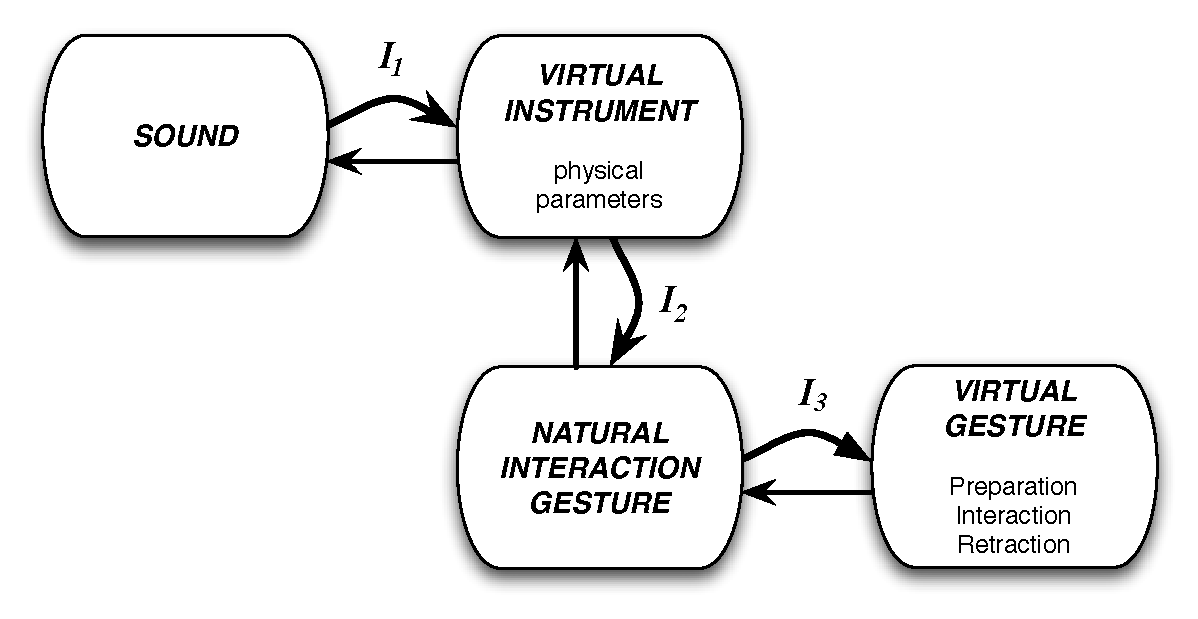
\includegraphics[width=0.6\textwidth]{Chapter4/Pics/Pdf/VirtualGesture.pdf}
%	\end{center}
%	\vspace{-1cm}
%	\caption{Inversion processes involved in the control of virtual instruments}
%	\label{fig:VMIs-VG}
%\end{figure}

%Our work takes place in the fact that there is a lack of knowledge on significant gestural characteristics that can be applied to virtual instruments producing sound. We therefore propose to go further and introduce a complete modeling of gesture, by designing a human-like character endowed with realistic and expressive behaviors. In order to reproduce the main characteristics of the control exerted on a real instrument, and more specifically the efforts involved in the interaction, we adopt a physics-based approach for modeling both the virtual performer and the sound-synthesis process (chapter \ref{chapter:Synthesis}). Such a physics modeling approach allows to represent not only what occurs during the mechanical interaction between the instrumentist and the instrument, but also the whole gesture production system, including the preparatory and the retraction phases that precede and follow the interaction process (\myfigname \ref{fig:VMIs-VG}, inversion $I_3$).

%Our work sensibly differs from the ones that use the gestural signals  directly responsible for the sound production \citeIPA{bevilacqua:NIME07}, as we build the physical model that produces these gestural signals. Such a modeling and simulation approach provides kinematics and dynamics information of the movement throughout the duration of the instrumental performance. It thus becomes possible to modify the biomechanical parameters of the virtual performer and change the simulated movement.\\

%However, without any real data, infering the forces and moments applied to joints and bones of the character still remains a difficult problem (inverse problem). We propose to solve it by using motion captured data recorded during real performances. The idea is to extract from these data a segmented and reduced-dimension representation of motion, and then to edit and assemble these motion chunks in order to control the virtual character. One key issue of our work is therefore to finely understand the underlying processes involved in the control of the virtual performer, and the way it is related to motion captured data recorded during real performances. In order to achieve these objectives, we highlight in an analysis process the significant dimensions of gesture that are involved when playing various percussion exercices. In particular we show that the mallet extremity trajectories may significantly characterize the gesture variations and may be used through an inversion process to control the virtual character.


%The main interest of a biomechanics-based modeling of gesture lies in the dynamical understanding of the mechanical links established between the instrumentist and the instrument. Furthermore, the physical approach may give some insight into the various parameters that are responsible for conducting specific performances with a desired expressivity. These parameters may characterize for example the joint constraints in the form of angular limits or biomechanical parameters such as stiffness, or damping of the joints. Finally, such a physics modeling approach allows to represent not only what occurs during the mechanical interaction between the instrumentist and the instrument, but also the whole gesture production system, including the preparatory and the retraction phases that precede and follow the interaction process (\myfigname \ref{fig:VMIs-VG}, inversion $I_3$).\\

%In the same way as the sound-synthesis research focuses on effect-centered (sampling and spectral modeling) or cause-centered (physical modeling) methods, the control of virtual characters involves either kinematics (effect-centered, see for instance \citeCGA{tolani:GM00}) or dynamics (cause-centered, for example \citeCGA{zordan:TOG05}) solutions. In order to take advantage of both methods, we define a cascaded combination of two inversion models (kinematics and dynamics) that allows to control the virtual performer through a sensorimotor control loop. This controller (\myfigname \ref{fig:gestureSoundProduction}) uses sensory informations (for example kinematic mallet trajectories or more generally visual information) to update the forces or torques that drive the muscular-skeleton model of the virtual performer. More related to musical gesture modeling, our work sensibly differs from the ones that use the gestural signals  directly responsible for the sound production \citeCM{bevilacqua:NIME07}, as we build the physical model that produces these gestural signals. Such a modeling and simulation approach provides kinematics and dynamics information of the movement throughout the duration of the instrumental performance. It thus becomes possible to modify the biomechanical parameters of the virtual performer and change the simulated movement.\\

%However, without any real data, infering the forces and moments applied to joints and bones of the character still remains a difficult problem (inverse problem). We propose to solve it by using motion captured data recorded during real performances. The idea is to extract from these data a segmented and reduced-dimension representation of motion, and then to edit and assemble these motion chunks in order to control the virtual character. One key issue of our work is therefore to finely understand the underlying processes involved in the control of the virtual performer, and the way it is related to motion captured data recorded during real performances. In order to achieve these objectives, we highlight in an analysis process the significant dimensions of gesture that are involved when playing various percussion exercices. In particular we show that the mallet extremity trajectories may significantly characterize the gesture variations and may be used through an inversion process to control the virtual character.

%\begin{figure}[H]
%	\begin{center}
%	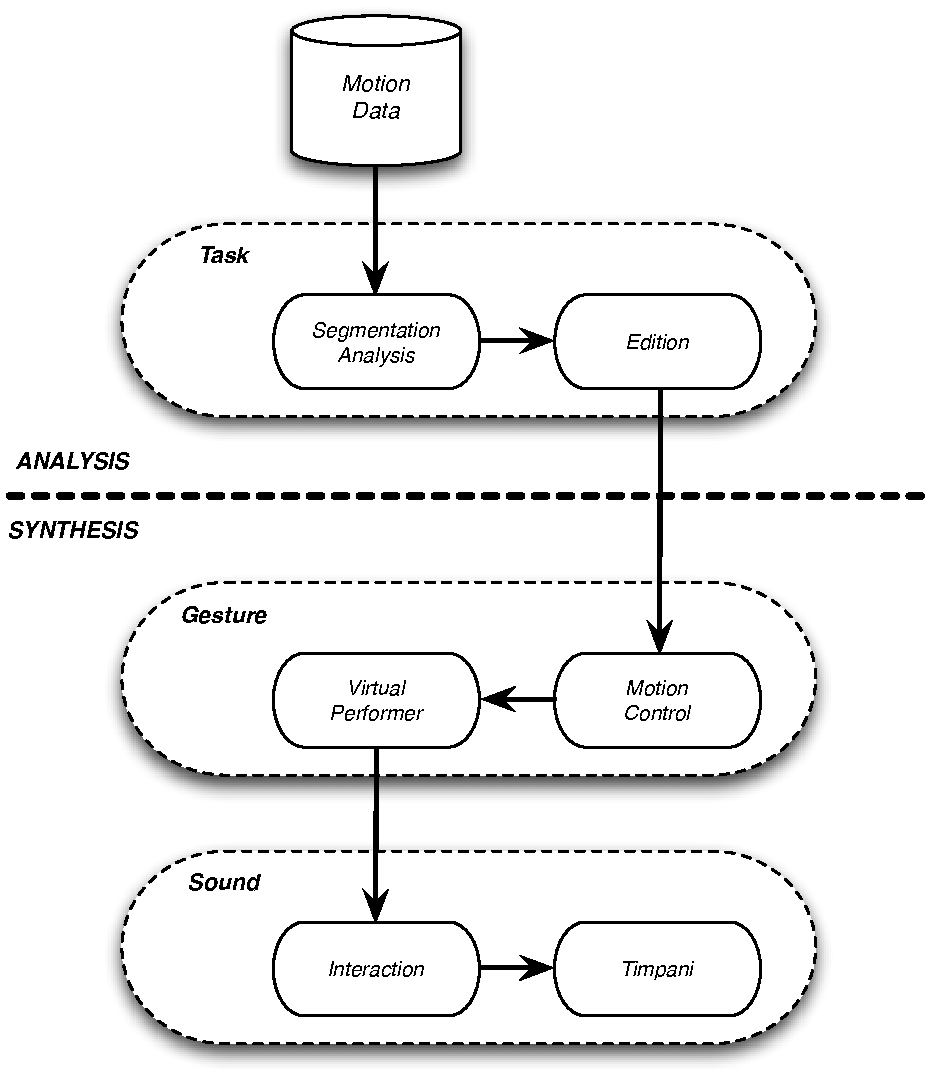
\includegraphics[width=0.6\textwidth]{./Data/Pdf/GeneralApproach-b&w.pdf}
%	\end{center}
%	\vspace{-1cm}
%	\caption{Gesture and sound production.}
%	\label{fig:gestureSoundProduction}
%\end{figure}

%The paper is organised as follows. Section \ref{sec:analysis} presents the extraction of a set of relevant parameters characterizing percussion performance, as well as its evaluation. We then propose a control method for synthesizing virtual percussion gestures in section \ref{sec:modelingControl}, based on the previous analysis stage. Results are then presented in section \ref{sec:results}; they concern both the evaluation of the synthesized gestures compared to real ones, and the visualization of the synthesized performances. We eventually conclude and draw perspectives of this work in section \ref{sec:conclusion}.

%%%%%%%%%%%%%%%%%%%%%%%%%%%%%%%%%%%%%%%%%%%%%%%%%%%%%%%%%%%%%%%%%%%%%%%%%%%%%%%%%%%%%%%%%%%%%%%%%%%%%%%%%%%%%%%%%%%%


%%%%%%%%%%%%%%%%%%%%%%%%%%%%%%%%%%%%%%%%%%%%%%%%%%%%%%%%%%%%%%%%%%%%%%%%%%%%%%%%%%%%%%%%%%%%%%%%%%%%%%%%%%%%%%%%%%%%

	\section{Timpani Basics}
	\label{sec:Analysis_TimpaniBasics}

There are many classifications of percussion instruments, one of the most established typologies is based on physical characteristics of instruments and the way by which they produce sound. According to this classification, timpani are considered as membranophones, "producing sound when the membrane or head is put into motion" \citeIPA{cook97}. Timpani are also called "kettledrums", and are considered as the first percussion instrument introduced in the composition of a classical orchestra more than 400 years ago \citeIPA{blades95}. The dramatic resounding and powerful effects that can emerge from the timpani makes this instrument one of most important percussion instrument in an orchestra.\\

In this subsection, we depict the basics for playing timpani, including the presentation of timpani-related equipments, acoustics properties of timpani sound properties, as well as its main playing techniques.


		\subsection{Equipment}
		\label{subsec:Analysis_TimpaniBasics_Equipment}

The equipment related to timpani is mainly composed of a bowl, a head and mallets as shown in \myfigname \ref{fig:timpaniEquipment}. In general, timpanists have to cope with several timpani (usually four) with bowls varying in size. The diameter of timpani membranes usually range from 23'' to 32'' \citeIPA{peters84} and players should properly tune each timpani to its corresponding pitch interval (\mytabname \ref{tab:timpaniPitch}).\\

As for timpani mallets, they consist of a shaft and a head. They are designed in various lengths, weights, thicknesses and materials \citeIPA{cook97} and their choice is of great importance \citeIPA{noak84}, namely depending on the percussionist level and on the task to be performed in the instrumental situation (low or fast rolls).

\begin{figure}%[H]
	\begin{center}
		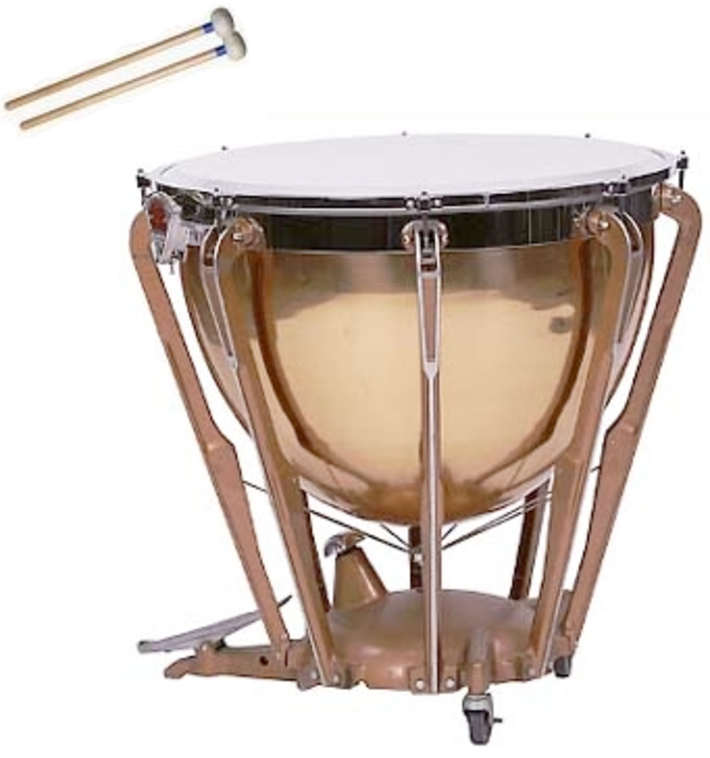
\includegraphics[width=0.4\columnwidth]{Chapters/4/Pics/Pdf/timpaniEquipment.pdf}
	\end{center}
	\vspace{-0.5cm}
	\caption[Timpani equipment]{Timpani equipment: bowl, membrane and mallets.}
	\label{fig:timpaniEquipment}
\end{figure}

\begin{table}%[H]
	\centering
	\caption[Bowl diameters and corresponding pitch intervals]{Bowl diameters and corresponding pitch intervals.}
	\vspace{2mm}
	\begin{tabular}{||x{3cm}||x{2cm}|x{2cm}|x{2cm}|x{2cm}||} \hline
		\small{$Bowl$ $diameter$} 	& $23''$ 	& $26''$ 	& $29''$ 	& $32''$	\tabularnewline \hline \hline
		\small{$Pitch$ $interval$} 	& $D3-A3$ 	& $B^b2-F3$ & $F2-C3$ 	& $D2-A2$	\tabularnewline \hline
	\end{tabular}
	\label{tab:timpaniPitch}
\end{table}


		\subsection{Acoustics}
		\label{subsec:Analysis_TimpaniBasics_Acoustics}

The acoustics of timpani percussion instruments has extensively been under study, mostly due to the timpani oddity known as the "missing fundamental" problem. The "missing fundamental" issue is well known among timpanists, this refers to the fact that a strike in the membrane center result in a muffled sound, so that the fundamental of timpani is considered to be the sound resulting from the '11' vibration mode rather than the '01' vibration mode (\myfigname \ref{fig:timpaniModes}). Other vibrating modes correspond to harmonics, such as the '21' and '31' modes which are respectively related to a fifth and a major seventh. It has been moreover shown that 'x1' vibration modes characterize predominant harmonic partials \citeIPA{rossing:SA82}. The "missing fundamental" issue can therefore be seen as a vibrating mode shift as the fundamental is shifted from the '01' mode to the '11'.\\

\begin{figure}[H]
	\begin{center}
		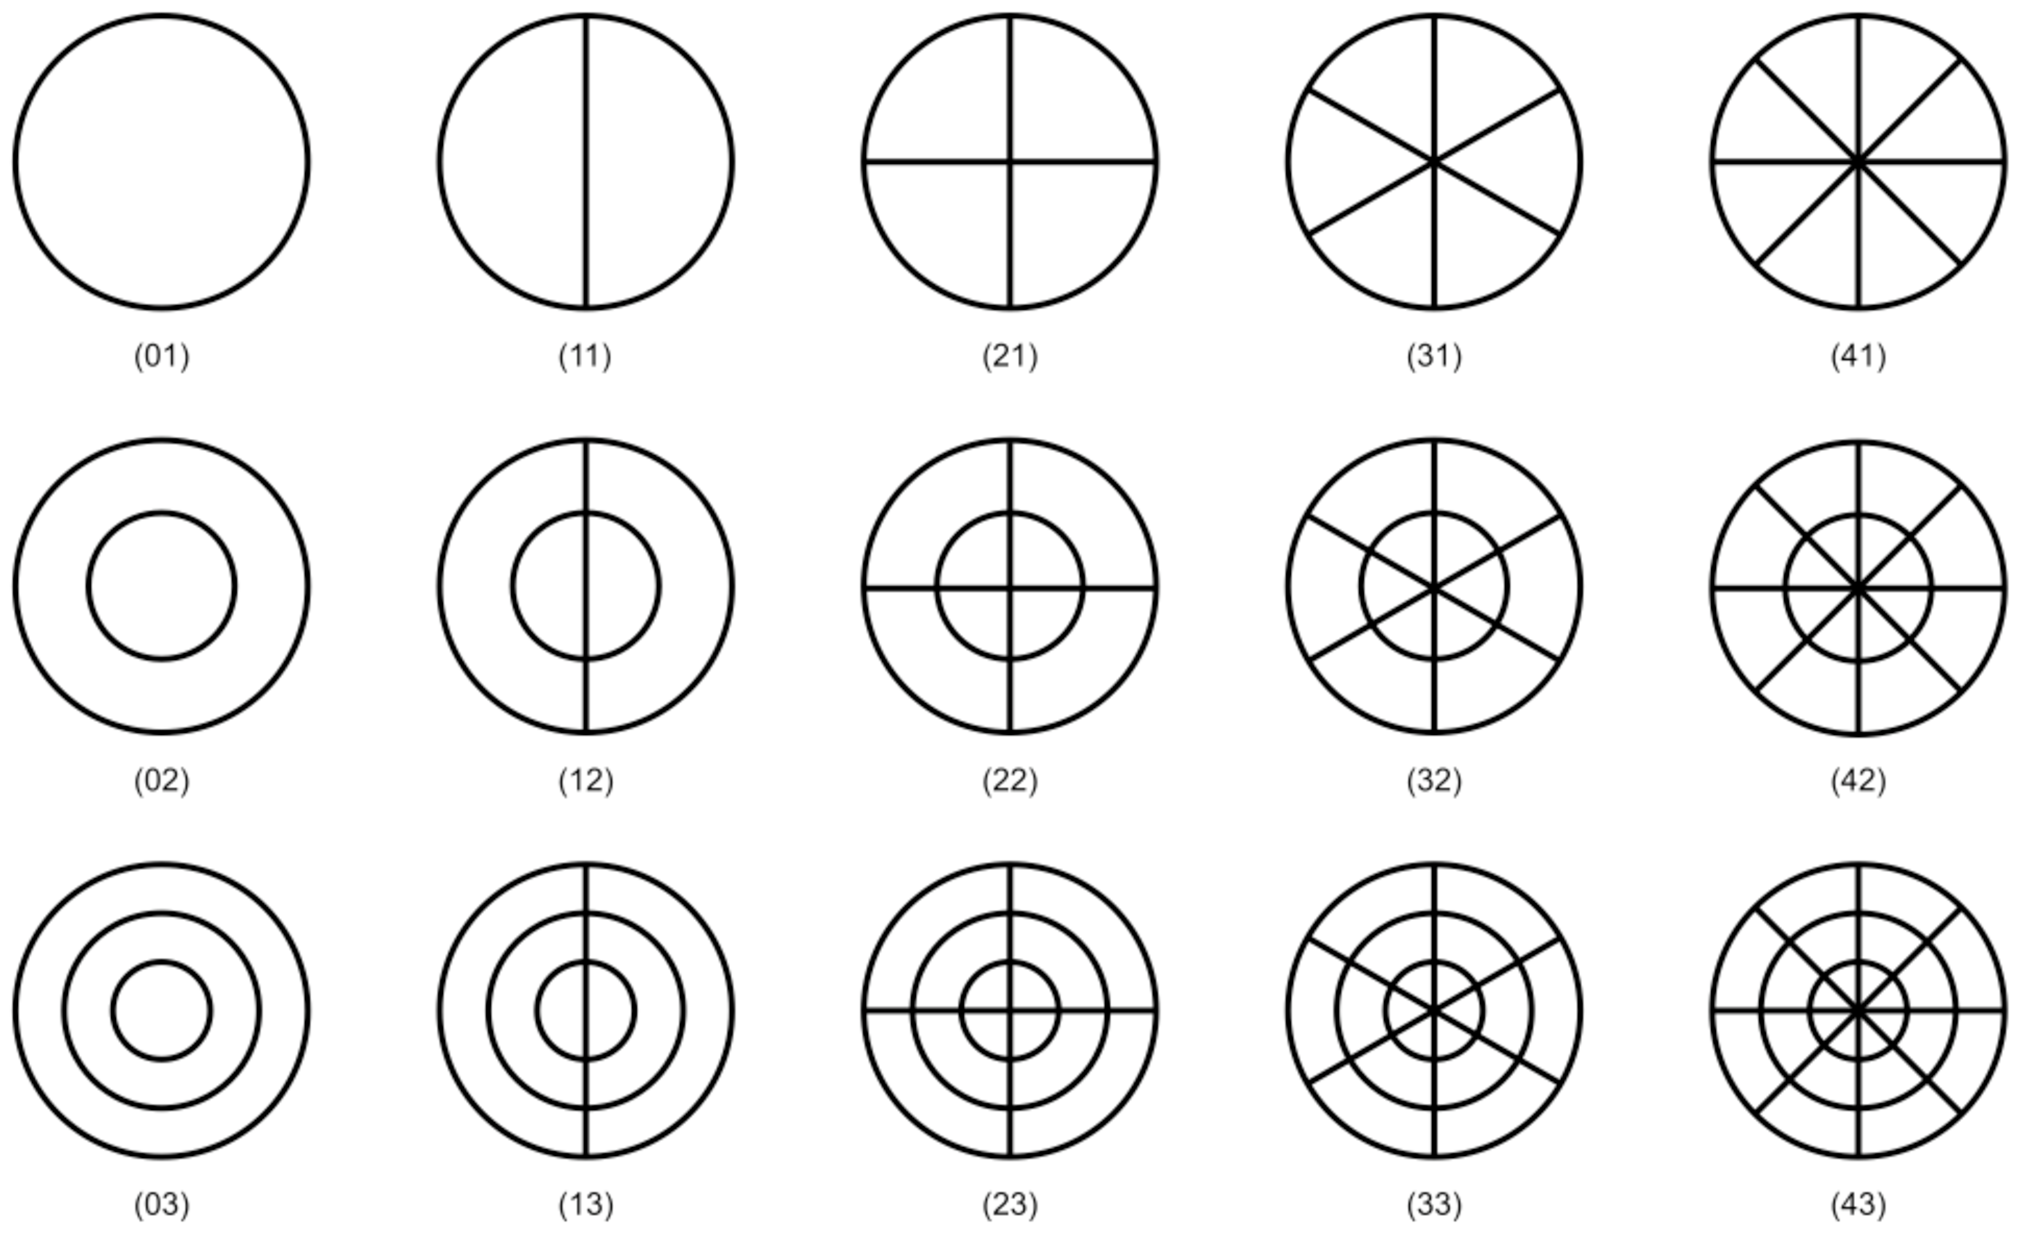
\includegraphics[width=0.8\columnwidth]{Chapters/4/Pics/Pdf/timpaniModes.pdf}
	\end{center}
	\vspace{-0.5cm}
	\caption[Vibrating modes of a timpani membrane]{Vibrating (x, y) modes of a timpani membrane, vertically (x) and horizontally (y)(courtesy of \citeIPA{rossing91}).}
	\label{fig:timpaniModes}
\end{figure}

\begin{figure}[H]
	\begin{center}
		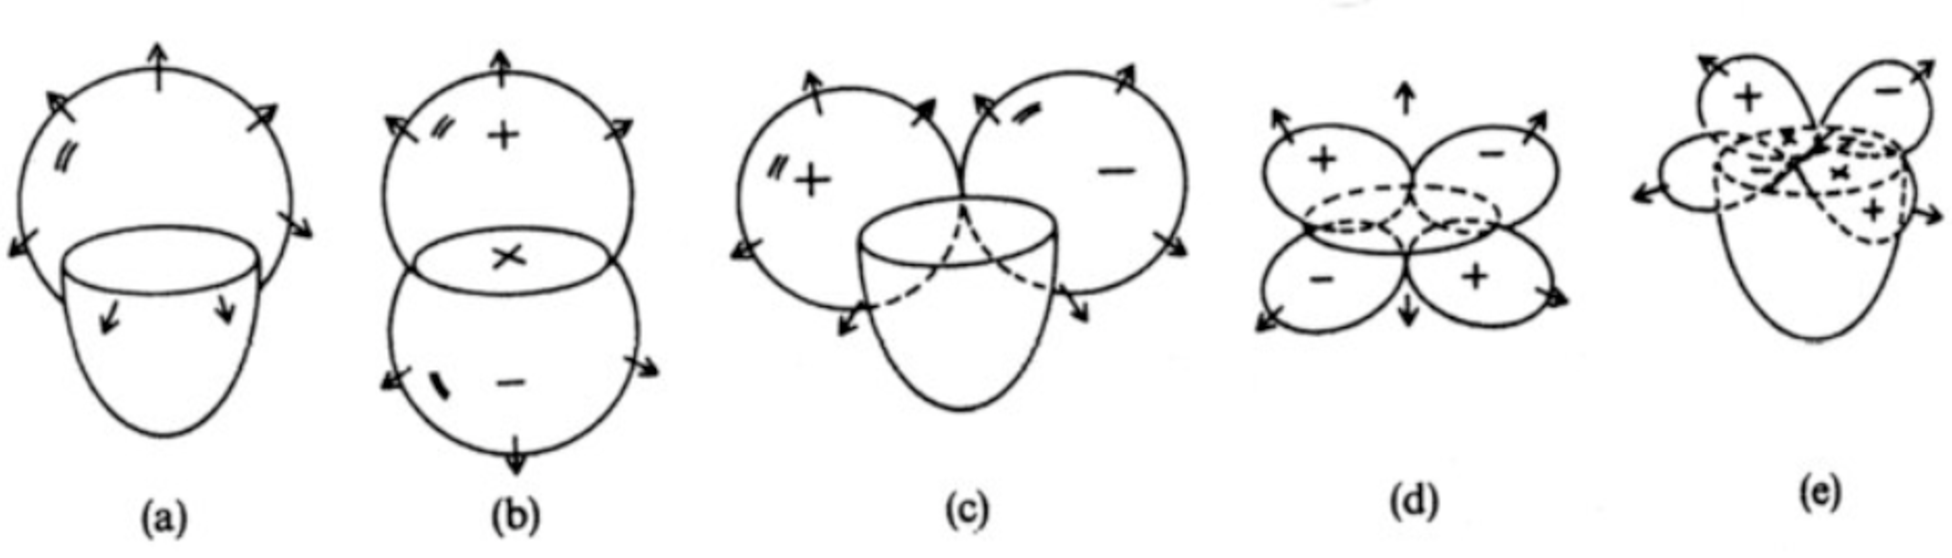
\includegraphics[width=0.8\columnwidth]{Chapters/4/Pics/Pdf/timpaniRadiationPoles.pdf}
	\end{center}
	\vspace{-0.5cm}
	\caption[Radiation poles of a timpani membrane]{Radiation poles of a timpani membrane: (a) monopole radiation of a baffled membrane in its (0, 1) mode, (b) dipole radiation of an unbaffled membrane in its (0, 1) mode, (c) dipole radiation of a baffled membrane in its (1, 1) mode, (d) quadrupole radiation of an unbaffled membrane in its (1, 1) mode, (d) quadrupole radiation of a baffled membrane in its (2, 1) mode (courtesy of \citeIPA{rossing91}).}
	\label{fig:timpaniRadiationPoles}
\end{figure}

The "missing fundamental" issue has also been explained in radiation terms. The most predominant phenomenon responsible of the vibrating mode shift is the air loading effect \citeIPA{rossing91} occuring in the timpani bowl. The radiated energy after a strike corresponding to the '01' is characterized by a monopole radiation scheme, so that the energy is radiated much more rapidly compared to other mode excitations (\myfigname \ref{fig:timpaniRadiationPoles}). Conversely other modes are radiating according to di- or quadrupoles that characterize lower radiation velocities.\\

The "missing fundamental" phenomenon is the reason why timpanists perform rarely a beat attack at the center of the timpani membrane. This observation is taken into account in our protocol for capturing timpani playing techniques, as we will see in the next section.

%\newpage


		\subsection{Playing Techniques}
		\label{subsec:Analysis_TimpaniBasics_Playing}

Timpani playing is characterized by a wide range of playing techniques, among them mallet grips as well as beat impact locations on the drum membrane are common features for differencing these techniques.\\

There are two main strategies for holding mallets, \myfigname \ref{fig:timpaniBasics1}: the \emph{French} grip (also called "thumbs-up") and the \emph{German} grip (or "matched" grip). These techniques imply different positions of the hand (vertical palm with the \emph{French} grip, horizontal with the \emph{German} grip), thus different motions of the wrist and of the fingers. 

Moreover, the use of the arms and forearms differ: broadly speaking, the \emph{French} grip asks for bigger amplitude in the use of the arms and forearms. It should be noted however that many timpanists use other techniques combining features from the two main techniques described here, or with a position of the wrist placing the palm at an angle of 45 degrees with the head of the timpani.\\

\begin{figure}%[H]
	\begin{center}
		\subfigure[]{\label{fig:timpaniBasics1}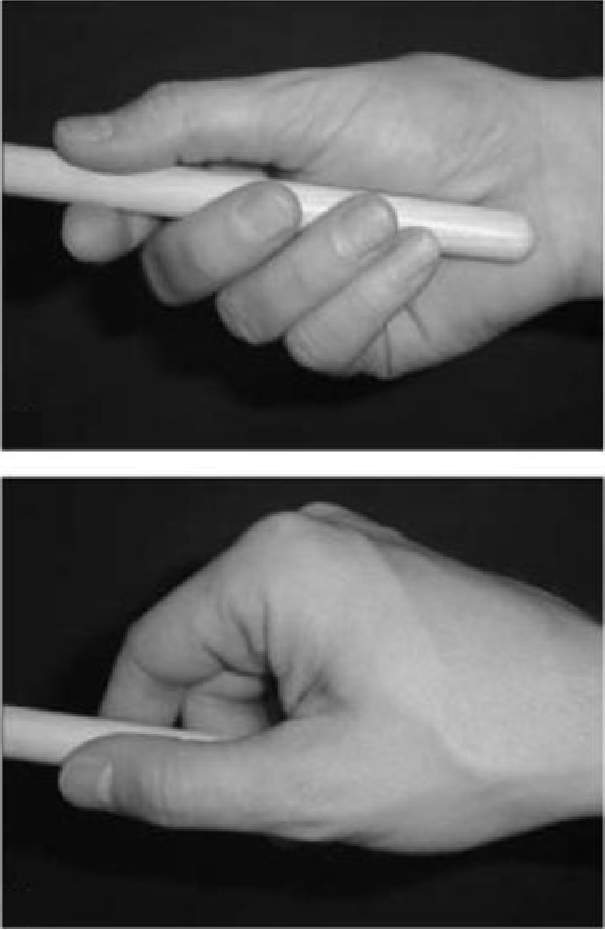
\includegraphics[width=0.25\columnwidth]{Chapters/4/Pics/Pdf/grips.pdf}}
		\subfigure[]{\label{fig:timpaniBasics2}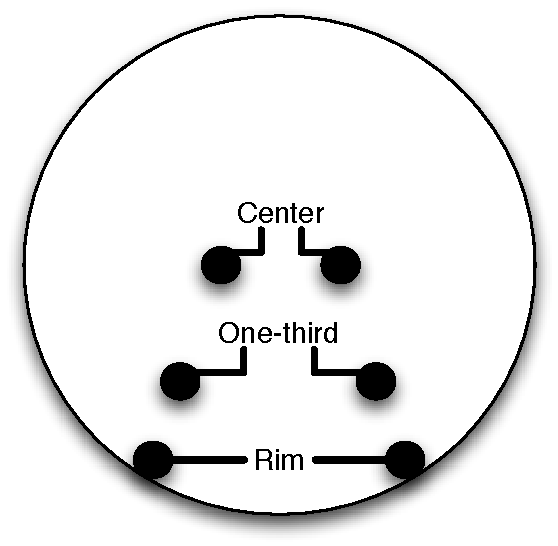
\includegraphics[width=0.35\columnwidth]{Chapters/4/Pics/Pdf/beatLocations2.pdf}}
	\end{center}
	\vspace{-0.5cm}
	\caption[Mallet grips and beat impact locations]{(a) \emph{French} (top) and \emph{German} (bottom) mallet grips. (b) Top view of the drum membrane: beat impact locations.}
	\label{fig:timpaniBasics}
\end{figure}

Moreover, players commonly use three distinct locations of impacts (\myfigname \ref{fig:timpaniBasics2}): \emph{One-third} of membrane radius, \emph{Center} and \emph{Rim} of the membrane. The most used is definitely the \emph{One-third} location, producing a full sound with a lot of resonance. The \emph{Center} location is characterized by a sharp and muffled attack with barely any resonance. And finally the \emph{Rim} location is characterized by a metallic sound and a resonance bringing mostly out high frequencies. These \emph{Center} and \emph{Rim} beat impact locations are used less often and have been adopted by composers after Eliot Carter's "Eight Pieces for Four Timpani" \citeIPA{carter68}.\\

\begin{figure}%[H]
	\begin{center}
		\subfigure[]{\label{fig:playingMode1}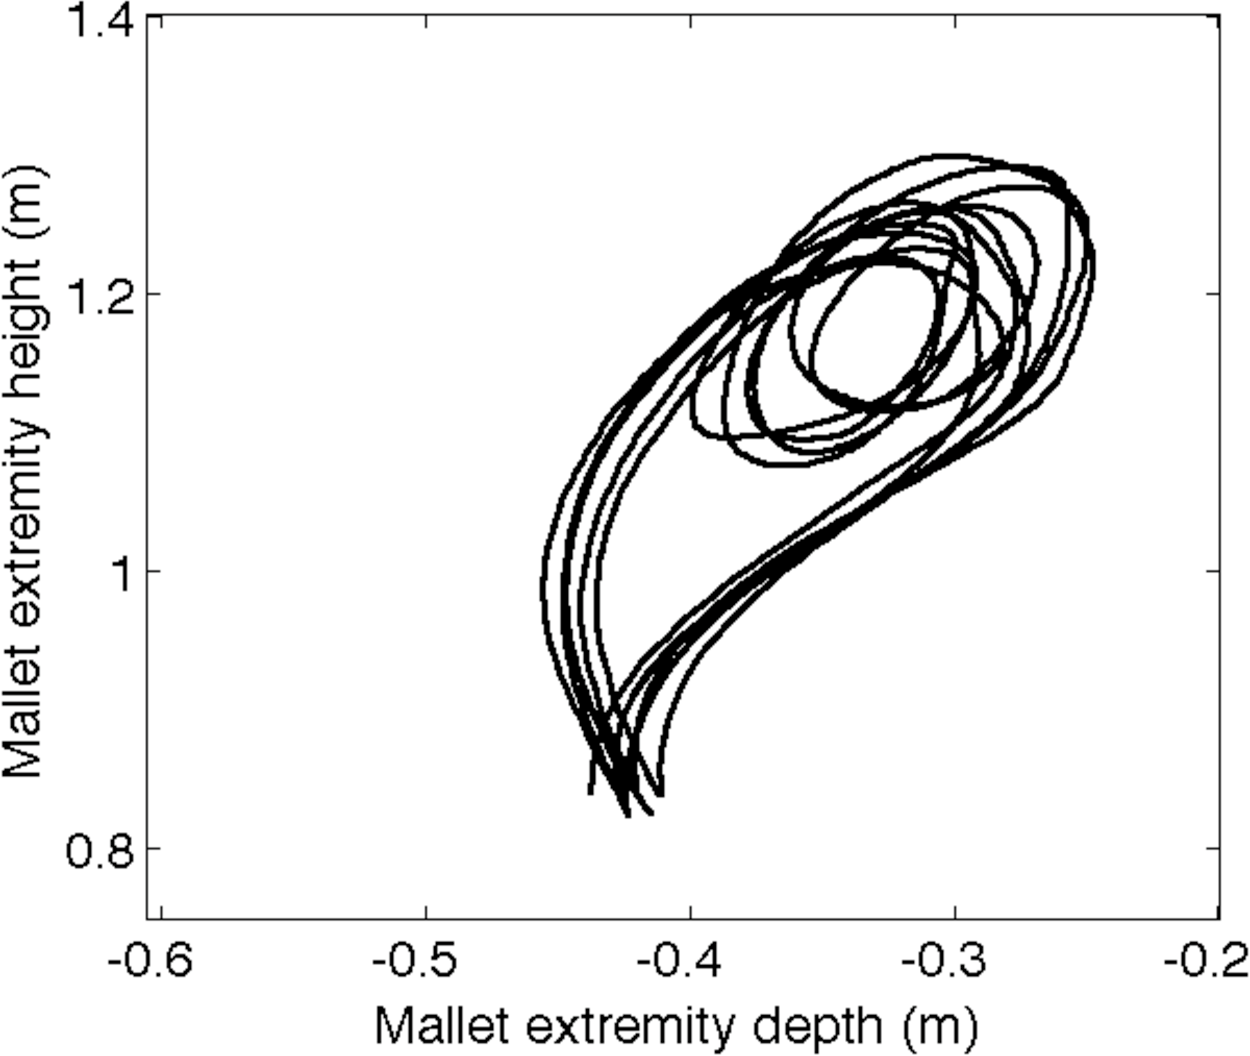
\includegraphics[width=0.45\linewidth]{Chapters/4/Pics/Pdf/legato.pdf}}
		\hspace{6mm}
		\subfigure[]{\label{fig:playingMode2}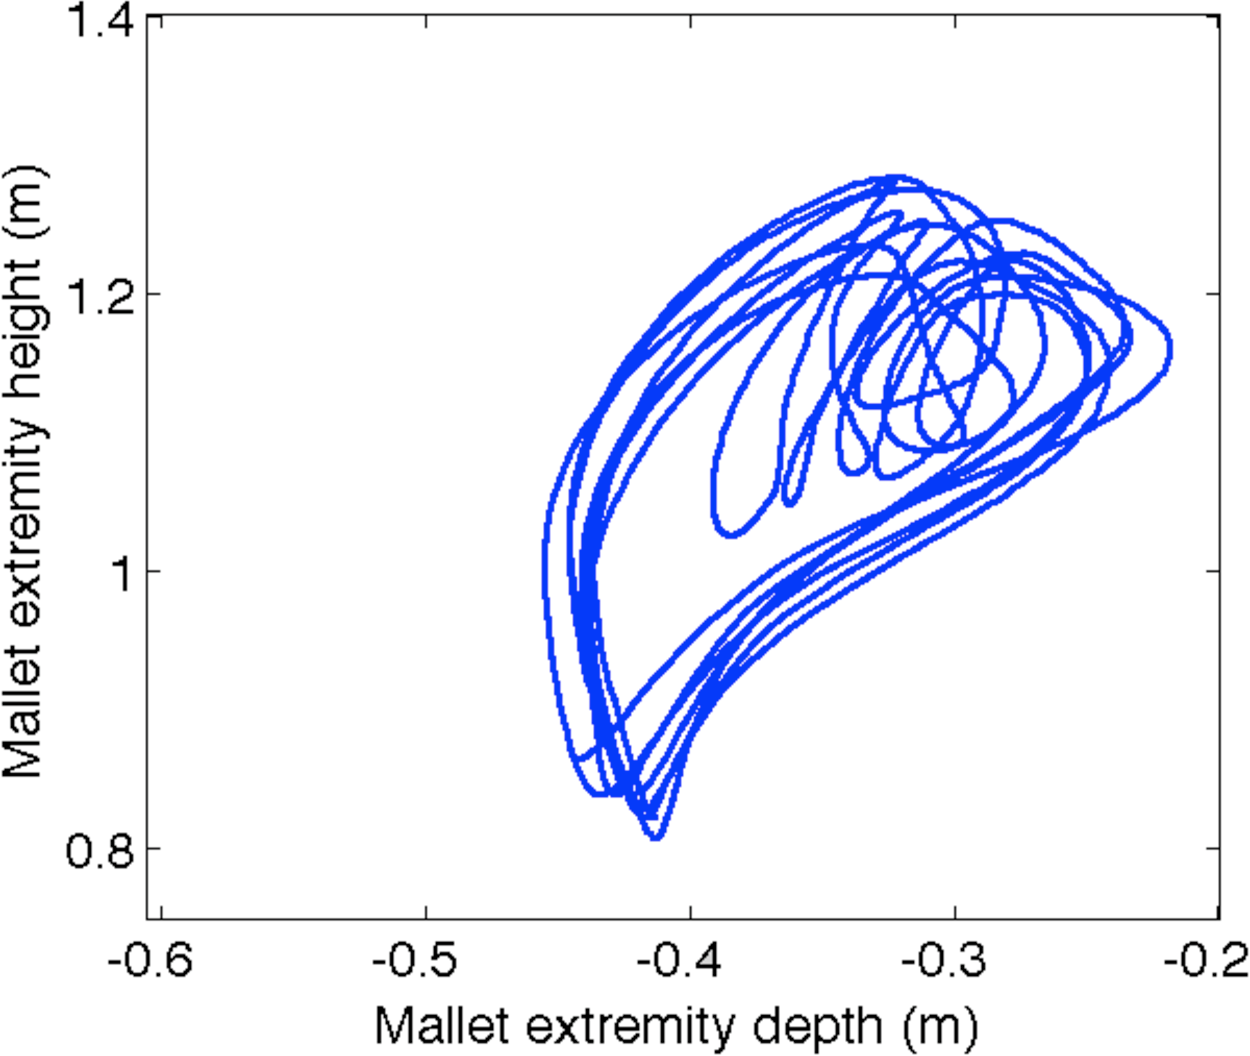
\includegraphics[width=0.45\linewidth]{Chapters/4/Pics/Pdf/tenuto.pdf}}\\
		\subfigure[]{\label{fig:playingMode3}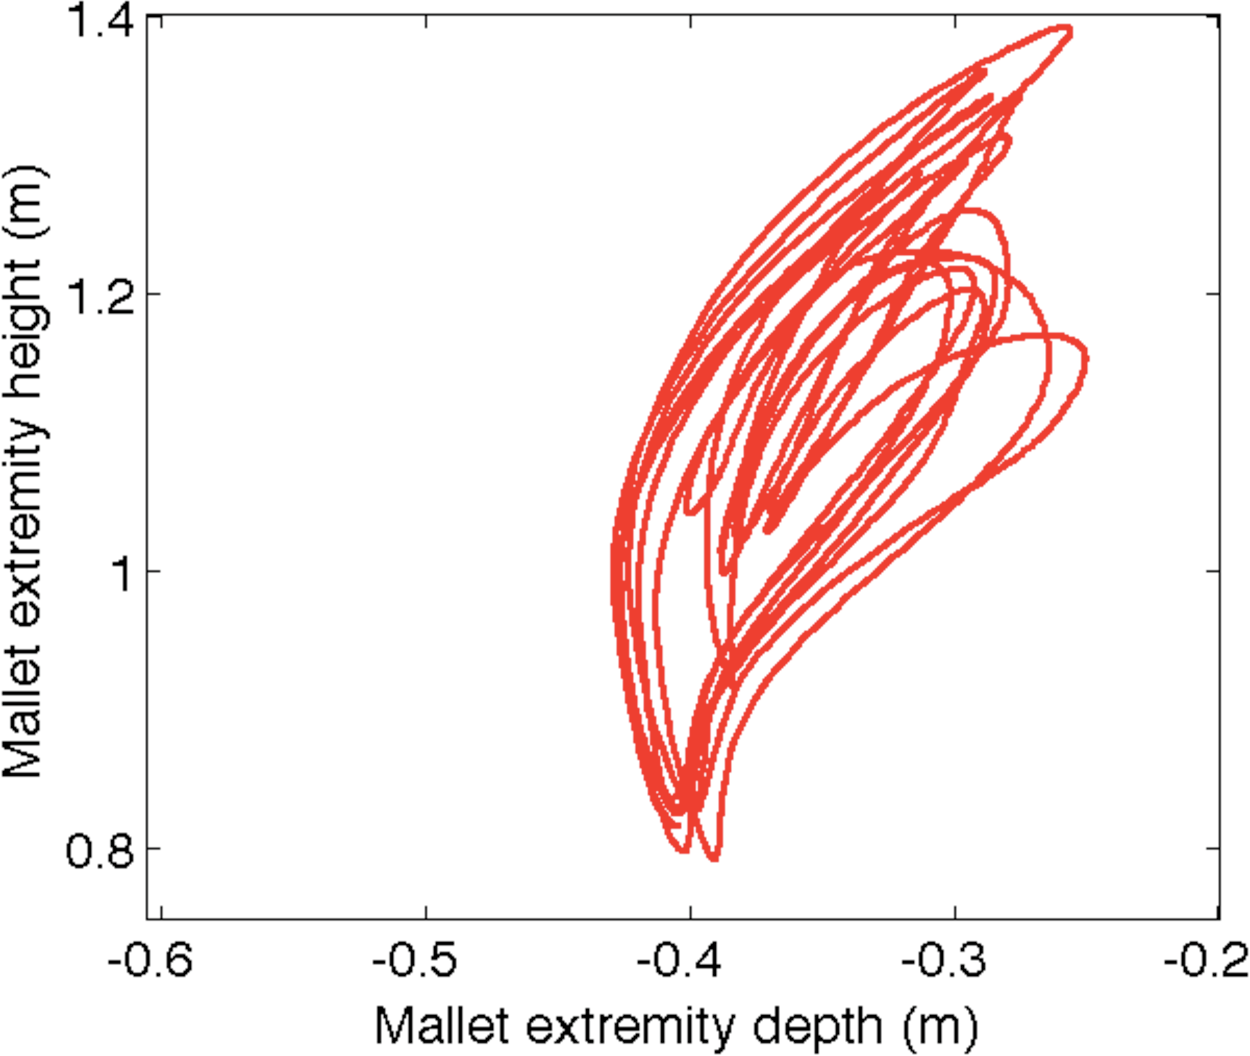
\includegraphics[width=0.45\linewidth]{Chapters/4/Pics/Pdf/accent.pdf}}
		\hspace{6mm}
		\subfigure[]{\label{fig:playingMode4}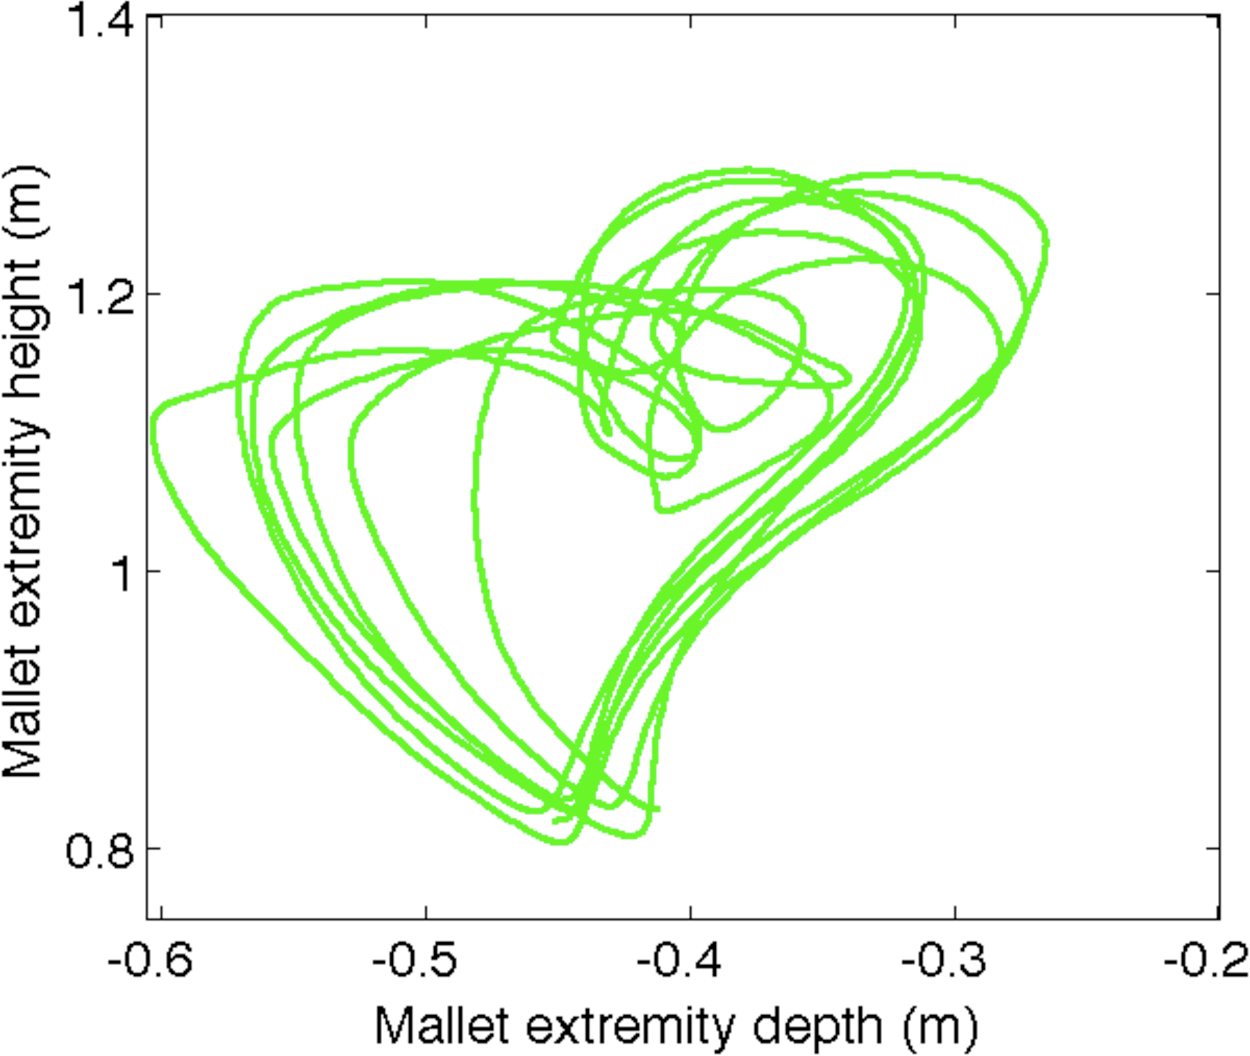
\includegraphics[width=0.45\linewidth]{Chapters/4/Pics/Pdf/verticalAccent.pdf}}\\
		\subfigure[]{\label{fig:playingMode5}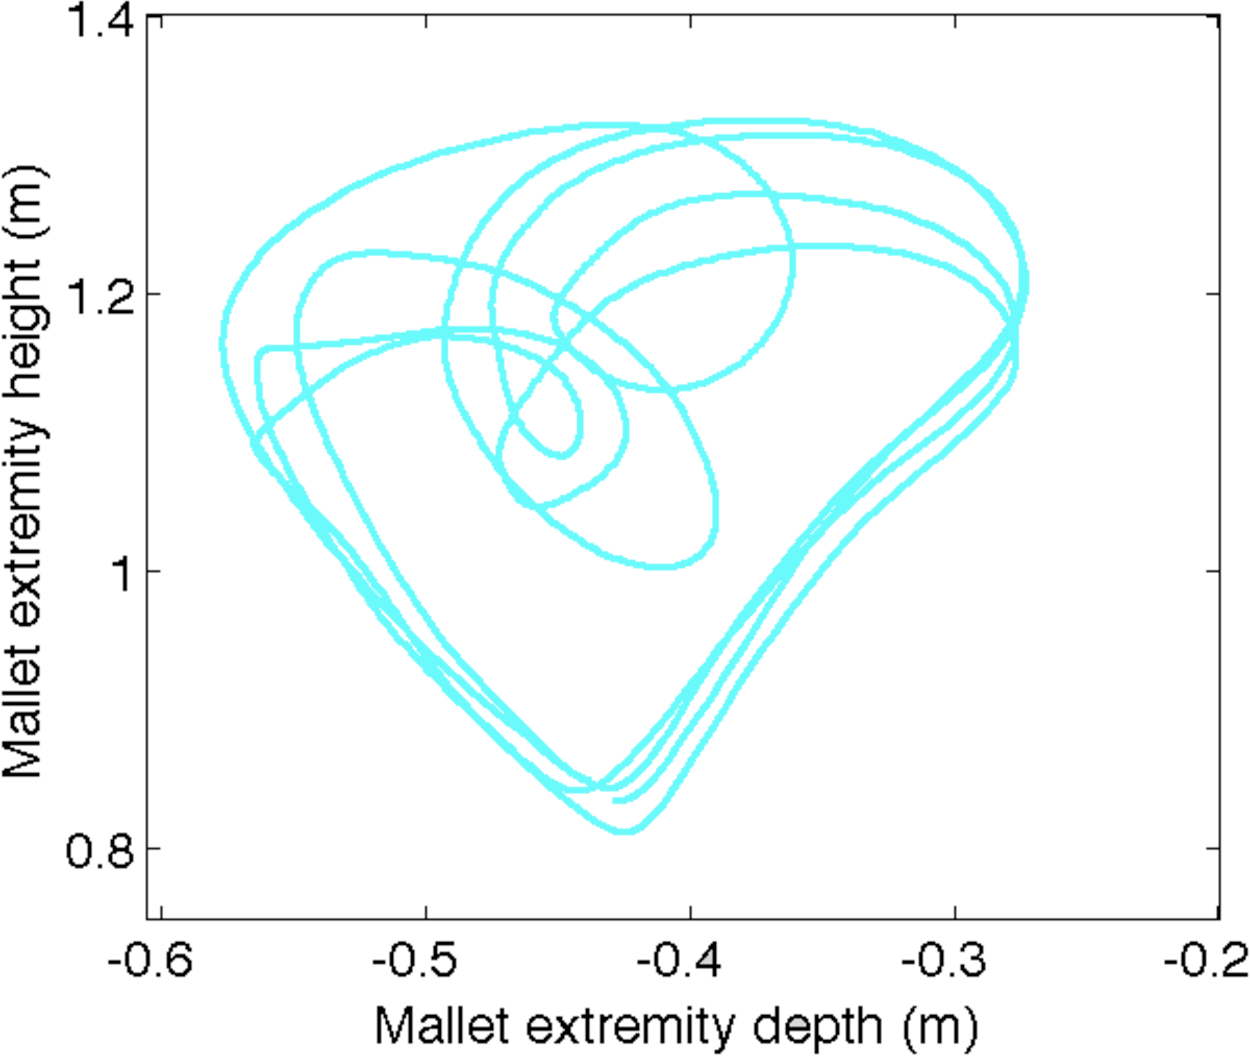
\includegraphics[width=0.45\linewidth]{Chapters/4/Pics/Pdf/staccato.pdf}}
	\end{center}
	\vspace{-0.6cm}
	\caption[Playing modes]{Mallet extremity trajectories in the sagital plane for the various playing modes: (a) \emph{legato}, (b) \emph{tenuto}, (c) \emph{accent}, (d) \emph{vertical accent}, (e) \emph{staccato}. The same color typology will be used further for representing these playing modes.}
	\label{fig:playingModes}
\end{figure}

Various playing modes can also been identified in timpani percussion performances. This includes different gesture variations, such as \emph{legato}, \emph{tenuto}, \emph{accent}, \emph{vertical accent} and \emph{staccato}. \myfigname \ref{fig:playingModes} depicts examples of these playing modes for the \emph{French} grip, through different profiles of mallet trajectories in the sagital plane.

A first observation leads to the identification of "air-beats" between two beat attacks, characterized by internal "loops" in the curves. These air-beats can be interpreted as a strategy from performers for keeping a regular tempo and counting the number of left and right beat attacks. It should be noted that these air-beats may not be present for recorded data at a higher tempo.

These playing modes show also different gesture dynamics, both in the longitudinal and vertical directions. While \emph{legato} and \emph{tenuto} playing modes are quite similar, \emph{accent} show a more stiff movement characterized by a bigger vertical amplitude, a lower longitudinal displacement, and therefore more constrained air-beats. Moreover, \emph{vertical accent} and \emph{staccato} shows a wider range of motion in the longitudinal direction, especially with a front projection of the mallet during the retractation phase (after the beat impact).\\

At a broader scale, whatever technique the timpanist is using, a compromise is generally found between the combined use of 1) the fingers, 2) the tightness of the grip on the shaft of the mallet, location of the grip on the mallet (depending of the length, diameter of the shaft and weight of the head of the mallet), 3) the position of the hand, 4) the amplitude and speed of the wrist, 5) the amplitude and speed of the forearms and arms, and eventually 6) the possibility or not to change the body's center of gravity (timpanist sitting down or standing up, the second position allowing the performer to use his whole body to control the weight, duration and velocity of the impact). 

%\newpage

%%%%%%%%%%%%%%%%%%%%%%%%%%%%%%%%%%%%%%%%%%%%%%%%%%%%%%%%%%%%%%%%%%%%%%%%%%%%%%%%%%%%%%%%%%%%%%%%%%%%%%%%%%%%%%%%%%%%


%%%%%%%%%%%%%%%%%%%%%%%%%%%%%%%%%%%%%%%%%%%%%%%%%%%%%%%%%%%%%%%%%%%%%%%%%%%%%%%%%%%%%%%%%%%%%%%%%%%%%%%%%%%%%%%%%%%%

	\section{Motion Capture Protocol and Database}
	\label{sec:Analysis_MoCapDatabase}


%		\subsection{Global Setup}
%		\label{subsec:Analysis_MoCapDatabase_MoCapSetup}

We captured the motion of several timpani performers by using a Vicon 460 system \citeCGA{vicon} based on Infra-Red camera tracking, as well as a standard DV camera that allow both the synchronization and retrieval of gesture and sound. Percussionists used a lycra suit fitted with markers placed according to the marker position of Vicon's \emph{Plug-in Gait}.  In order to retrieve beat impacts, markers have also been placed on the mallets. It should be noted that the placement of markers on mallets can have an impact on the recorded performance since it can slightly change their balance. The balance between left and right mallets can also be altered since different placements have been used, as a mean of recognizing left and right mallets during the post-processing phase of motion data. A careful choice of the size of the timpani has been done as regards to capture conditions. A 23'' timpani has therefore been used in order to minimize the occlusion of markers by the timpani bowl.\\

\begin{figure}%[H]
	\begin{center}
		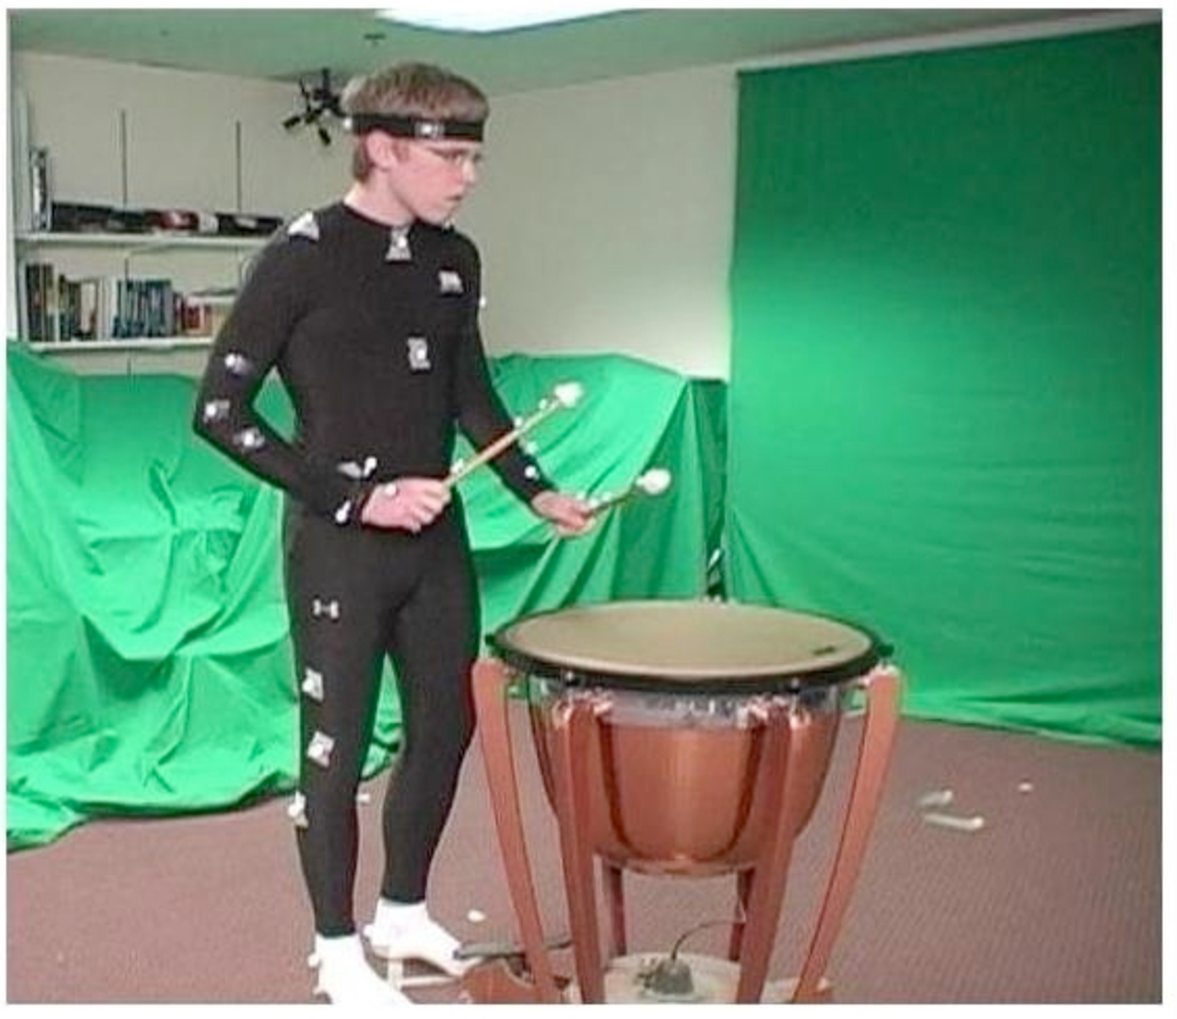
\includegraphics[height=60mm]{Chapters/4/Pics/Pdf/mocapSubject.pdf}
	\end{center}
	\vspace{-0.5cm}
	\caption[Timpani performer and the motion capture setup]{Timpani performer and the motion capture setup.}
	\label{fig:mocapSubject}
\end{figure}

Three percussionists (c.f. \myfigname \ref{fig:mocapSubject}) were asked to perform a pre-defined capture protocol consisting of a single stroke roll for each gesture (\emph{legato}, \emph{tenuto}, \emph{accent}, \emph{vertical accent} and \emph{staccato}). The capture protocol given to performers is provided in appendix \ref{chapter:MoCap}, as well as the corresponding ethical form.

For each gesture, performers were asked to change the location of the beat impact according to the three locations described in subsection \ref{sec:Analysis_TimpaniBasics}. In total, fifteen examples of timpani exercises were performed for each percussionist (each with five beats per hand).

\mytabname \ref{tab:mocapDatabase} presents a summary of the playing characteristics for each performer. The main differences across performers lie in their degree of expertise (\emph{B.A. student}, \emph{M.A. student} or \emph{Prof.}), the grip strategy used (\emph{French} or \emph{German}), their dominant (\emph{Left} or \emph{Right}) hand, and gender.\\

\begin{table}%[H]
	\centering
	\caption[MoCap subjects playing characteristics]{Subjects playing characteristics.}
	\vspace{2mm}
	\begin{tabular}{||x{2cm}||x{2cm}|x{2cm}|x{2cm}|x{2cm}||} \hline
		\small{$Features$ / $Subject$} & \small{$Expertise$} & \small{$Grip$} & \small{$Hand$} & \small{$Gender$} \tabularnewline \hline \hline
		\small{$S_1$} & \small{Prof.} 	& \small{French} 	& \small{Right} 	& \small{M} \tabularnewline \hline
		\small{$S_2$} & \small{B.A.}	& \small{German} 	& \small{Left}	 	& \small{M} \tabularnewline \hline
		\small{$S_3$} & \small{M.A.}	& \small{German} 	& \small{Right} 	& \small{F} \tabularnewline \hline
	\end{tabular}
	\label{tab:mocapDatabase}
\end{table}


%		\subsection{Choice of Sampling Rate}
%		\label{subsec:Analysis_MoCapDatabase_SamplingRate}

One of the main issues using such hardware solutions is the choice of the sampling rate used for the capture of percussive gestures (because of the short duration of the beat impact \citeIPA{dahl97, wagner:MsC06}).

With a high sampling rate (500 Hz and above), one can expect to more accurately retrieve beat attacks, but the spatial range is significantly reduced so that it may be difficult to capture the whole body of the performer.  For this project, a compromise was chosen by setting the cameras at 250 Hz, allowing both full-body capture as well as a reasonably high sampling rate for capturing reliably mallet beat impacts. 


%		\subsection{Motion Database Refinement: Segmentation}
%		\label{subsec:Analysis_MoCapDatabase_Segmentation}

%%%%%%%%%%%%%%%%%%%%%%%%%%%%%%%%%%%%%%%%%%%%%%%%%%%%%%%%%%%%%%%%%%%%%%%%%%%%%%%%%%%%%%%%%%%%%%%%%%%%%%%%%%%%%%%%%%%%


%%%%%%%%%%%%%%%%%%%%%%%%%%%%%%%%%%%%%%%%%%%%%%%%%%%%%%%%%%%%%%%%%%%%%%%%%%%%%%%%%%%%%%%%%%%%%%%%%%%%%%%%%%%%%%%%%%%%

	\section{Analysis}
	\label{sec:Analysis_TimpaniAnalysis}

We present here the analysis of timpani performance gestures collected in our database. This analysis focuses on the study of the trace of the percussionist action during musical performance: mallet extremity trajectories. As it can be intuitively stated \citeIPA{bouenard:ENACTIVE08}, percussionists more specifically control the motion of mallets over time. The aim of the following analysis is to provide a quantitative analysis of this hypothesis, as well as giving relevant parameters that are of particular interest for the modeling and synthesis part of our work (chapter \ref{chapter:Synthesis}). In order to highlight this assumption, we conduct below a study which aims at putting in evidence the effect of grips and playing modes on preparatory trajectories of mallet extremity.


		\subsection{Segmentation of Motion Capture Data}
		\label{subsec:Analysis_TimpaniAnalysis_Segmentation}

A refinement to the raw data contained in the motion capture database has been achieved as a first step of analyzing the effect of grips and playing modes on timpani preparatory gestures. As originally underlined in \citeCM{gibet:PhD87, ramstein:PhD91}, these gestural units may be obtained by the physical activity of the performer-instrument interaction (in our case beat impacts during percussion performances). We segment each percussion sequence that has been initially recorded into \emph{beat-to-beat} gesture units. These latter have been identified by processing a detection of beat impacts on mallet height trajectories. \myfigname \ref{fig:beatDetection} depicts a semi-automatic process for, firstly detecting local extrema on mallet trajectories that are potentially beat impacts, and secondly select manually the points of interest. Once \emph{beat-to-beat} gesture units are available for the playing techniques under study (grips and playing modes), it is possible to conduct a fine analysis of the effect of the playing techniques on mallet trajectories.

\begin{figure}%[H]
	\begin{center}
		\subfigure[]{\label{fig:beatDetection1}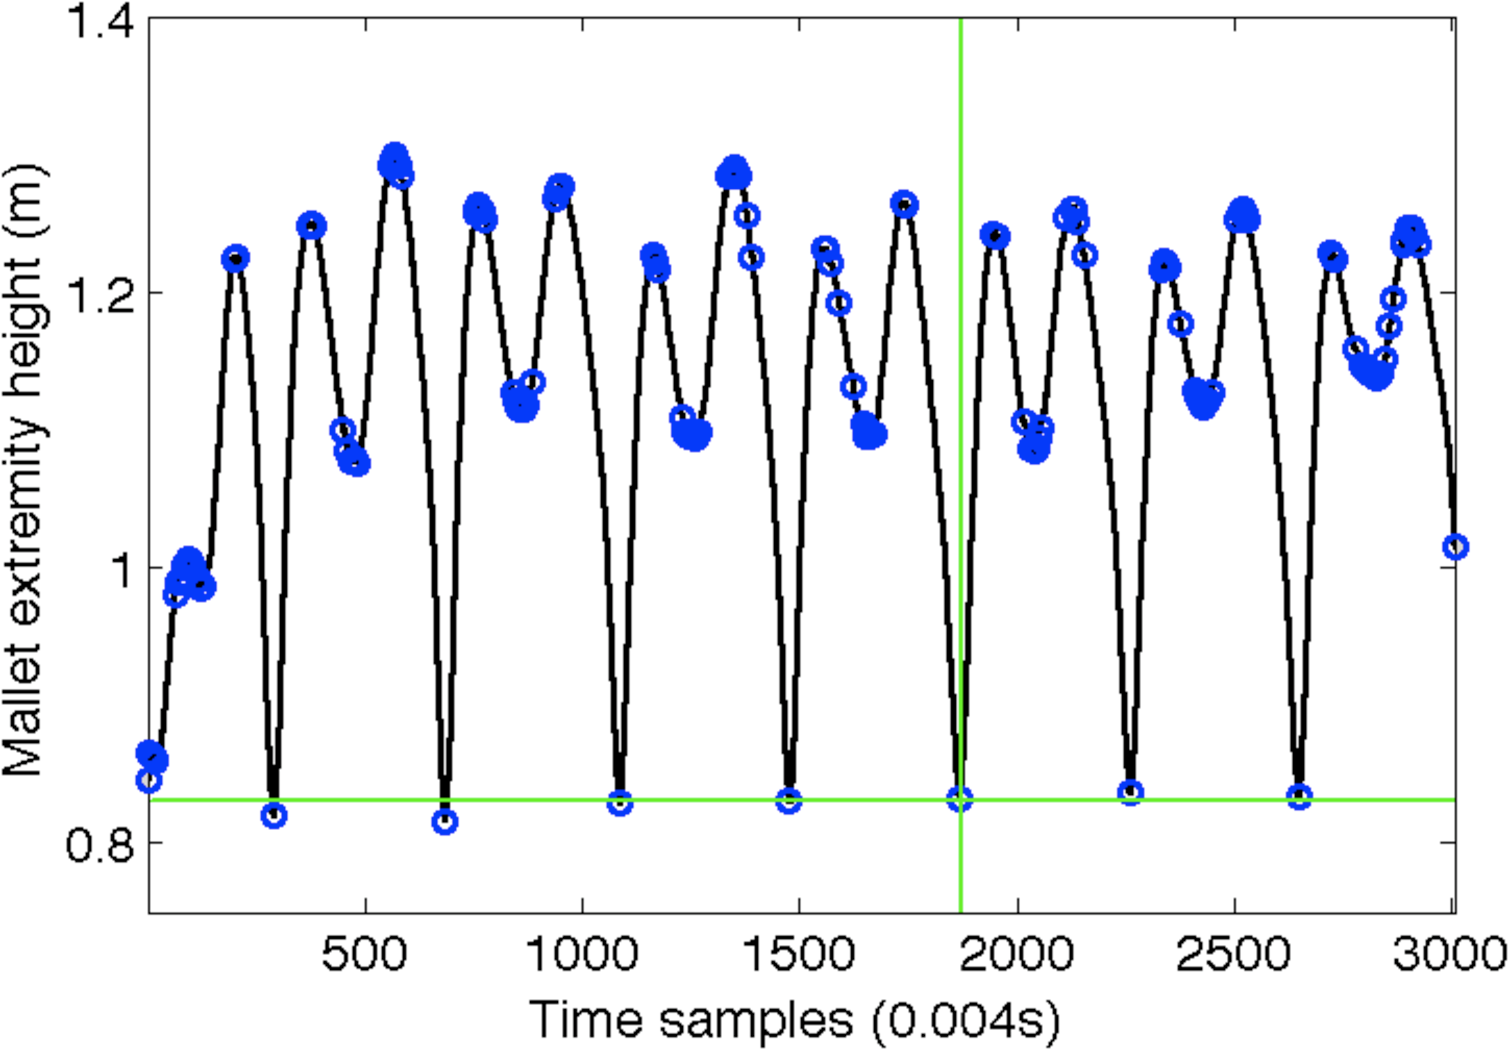
\includegraphics[width=0.495\linewidth]{Chapters/4/Pics/Pdf/beatDetection.pdf}}
		\subfigure[]{\label{fig:beatDetection2}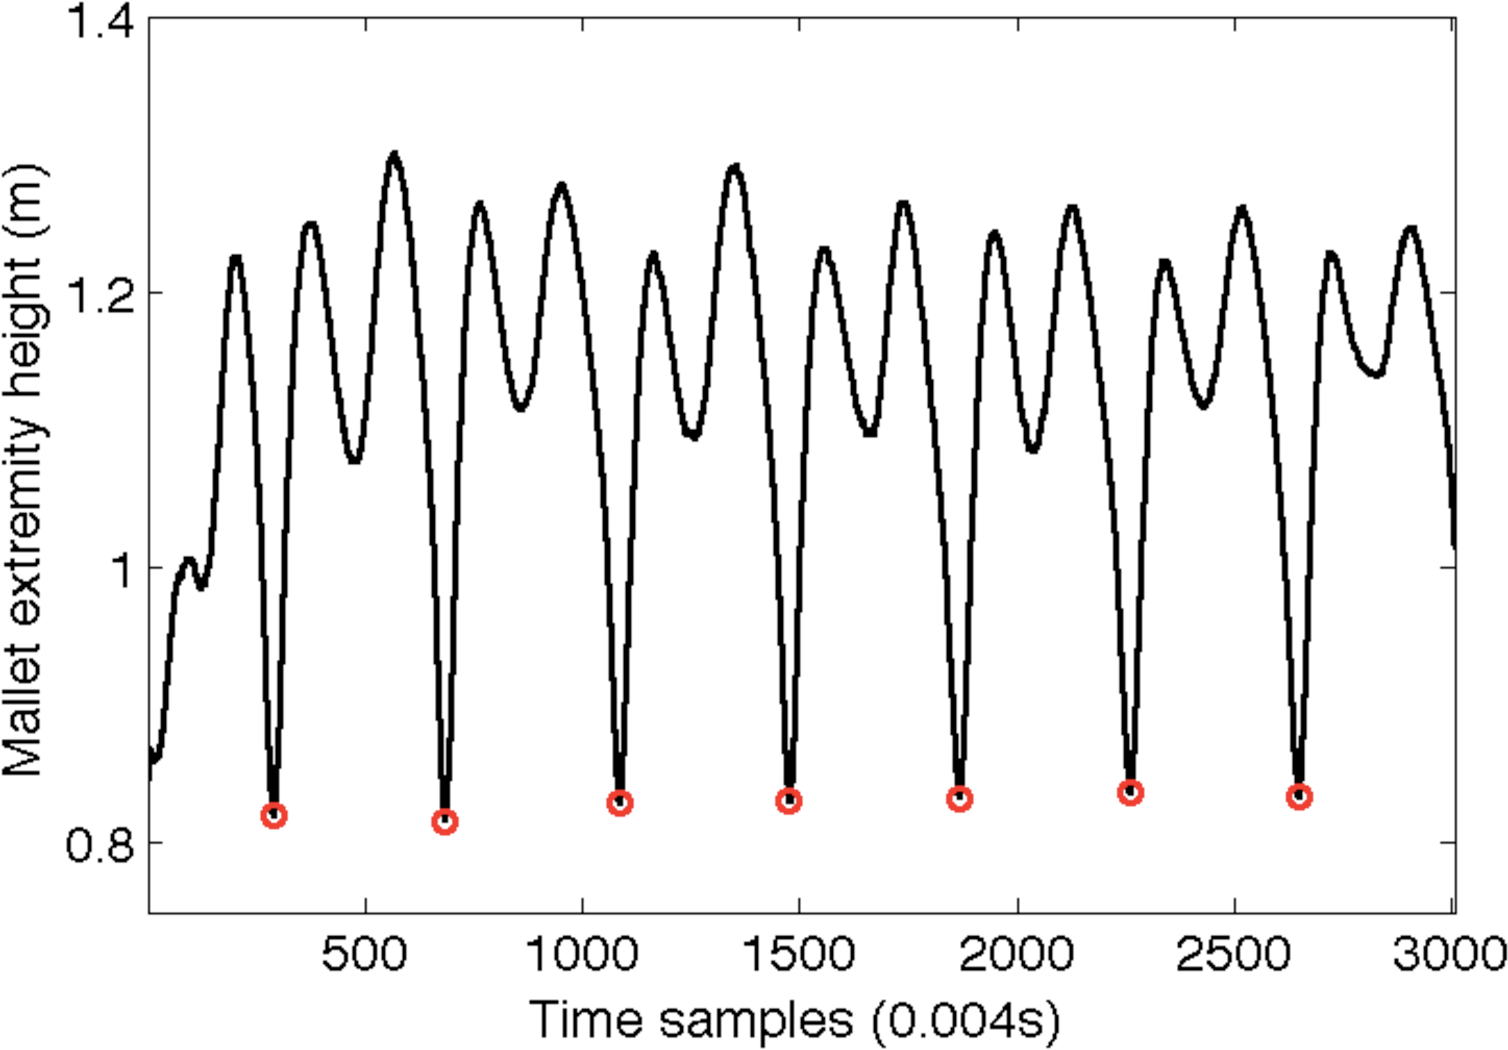
\includegraphics[width=0.495\linewidth]{Chapters/4/Pics/Pdf/beatDetection2.pdf}}
%		\subfigure[]{\label{fig:beatDetection1}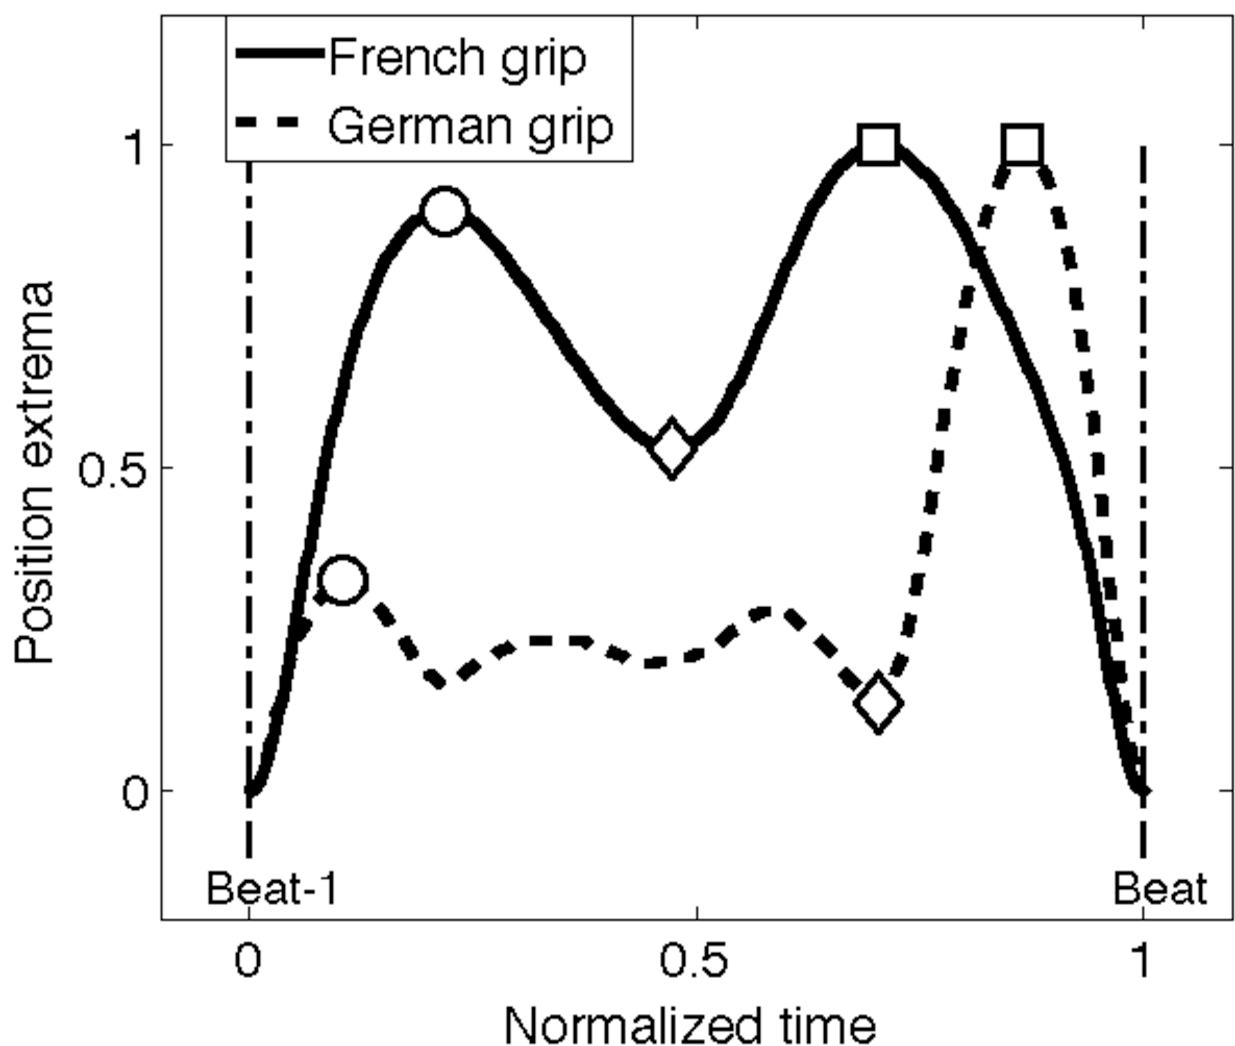
\includegraphics[width=0.45\linewidth]{Chapters/4/Pics/Pdf/pos_parameters.pdf}}
%		\hspace{6mm}
%		\subfigure[]{\label{fig:beatDetection2}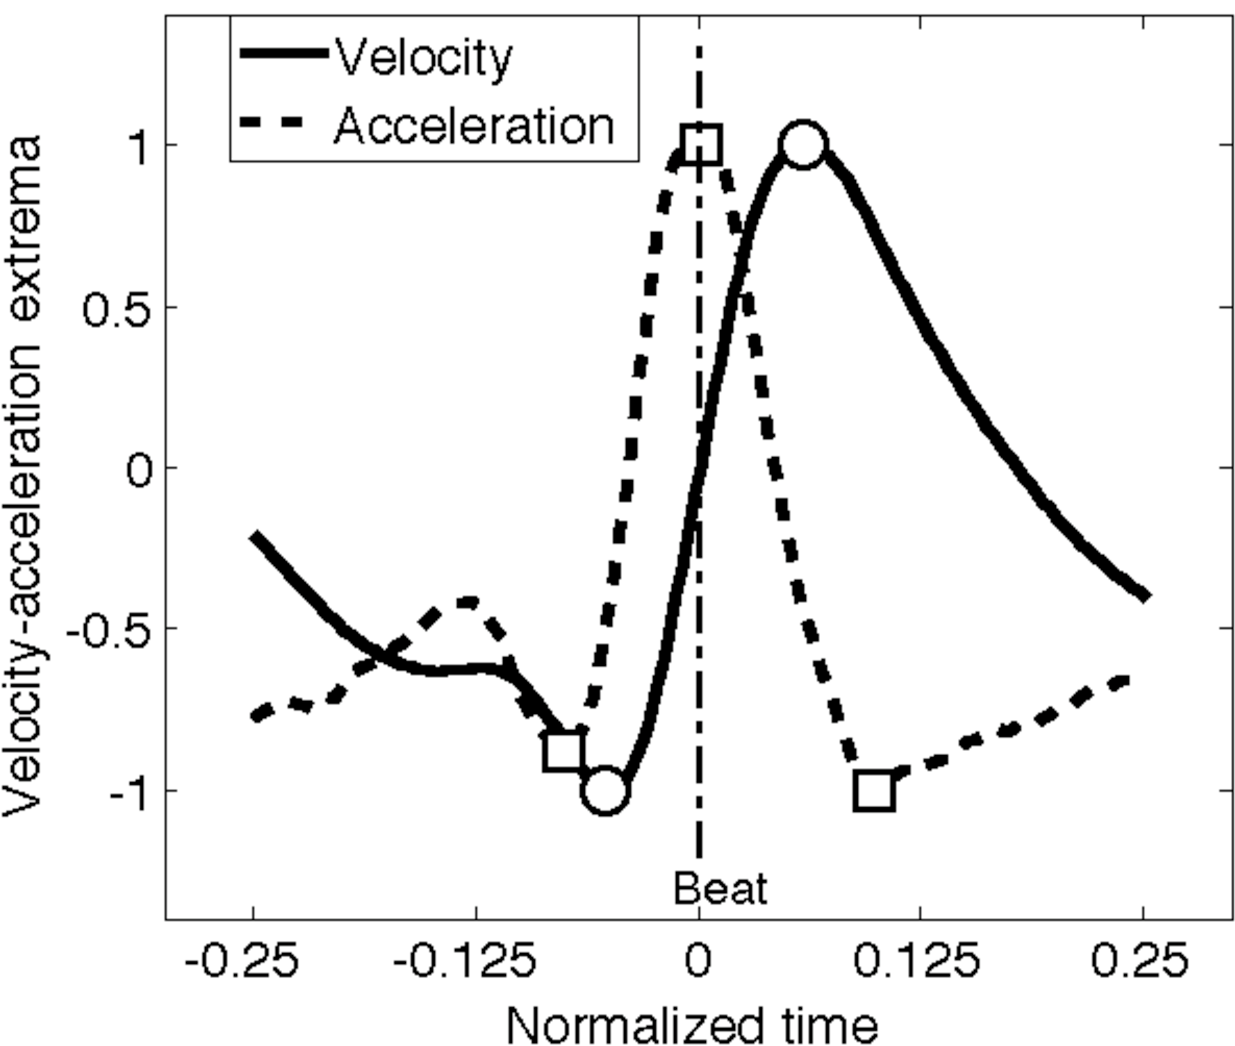
\includegraphics[width=0.45\linewidth]{Chapters/4/Pics/Pdf/vel_acc_parameters.pdf}}
	\end{center}
	\vspace{-0.6cm}
	\caption[Semi-automatic detection of beat impacts]{Semi-automatic detection of beat impacts: (a) detection of local extrema (blue circles) and selection (green cross) of points of interest, (b) resulting beat impacts (red circles).}
	\label{fig:beatDetection}
\end{figure}
		

		\subsection{Methodology}
		\label{subsec:Analysis_TimpaniAnalysis_Methodo}

The parameters used to characterize mallet trajectories are local extrema extracted from position trajectories during \emph{beat-to-beat preparatory} phases (\myfigname \ref{fig:classifParameters1}), as well as local extrema from velocity and acceleration \emph{beat-centered} profiles (\myfigname \ref{fig:classifParameters2}). Each playing mode for a particular grip is represented by a vector of sixteen dimensions, which correspond to the eight amplitude parameters presented in \myfigname \ref{fig:classifParameters} with their corresponding temporal occurence. These parameters are extracted automatically, therefore building a low-dimension representation of grips and playing modes. \myfigname \ref{fig:profiles} depict examples of position, velocity as well as acceleration trajectories for the various playing modes for both \emph{French} and \emph{German} grips.\\ %One can notice that velocity and acceleration parameters may be useful to distiguish a playing mode from another.\\

The evaluation of such a parameterization is conducted by a quantitative analysis based on a classification/recognition scheme. The relevance of these parameters is measured using the Support Vector Machine (\emph{SVM}) classification method, with the use of Radial Basis Functions (\emph{RBF}) as kernel functions. The scope of this evaluation concerns firstly parameters related to percussion grips (\emph{French} or \emph{German}), and secondly playing modes (\emph{legato}, \emph{tenuto}, \emph{accent}, \emph{vertical accent} and \emph{staccato}). For each case, a combination of parameters is chosen and forms a refined data set of the motion capture database, on which the classification/recognition will work. This refined data set is then divided into two sub-sets, an exerpt of it is randomly extracted to represent determined classes that train a classifier, whereas the remaining data represent queries submitted to the classifier. The relevance of the selected parameters is then estimated according to their recognition success by the classifier. In this quantitative study, the determined classes to recognize typically correspond to two classes for percussion grips, and five classes for playing modes.

\begin{figure}%[H]
	\begin{center}
%		\subfigure[]{\label{fig:classifParameters1}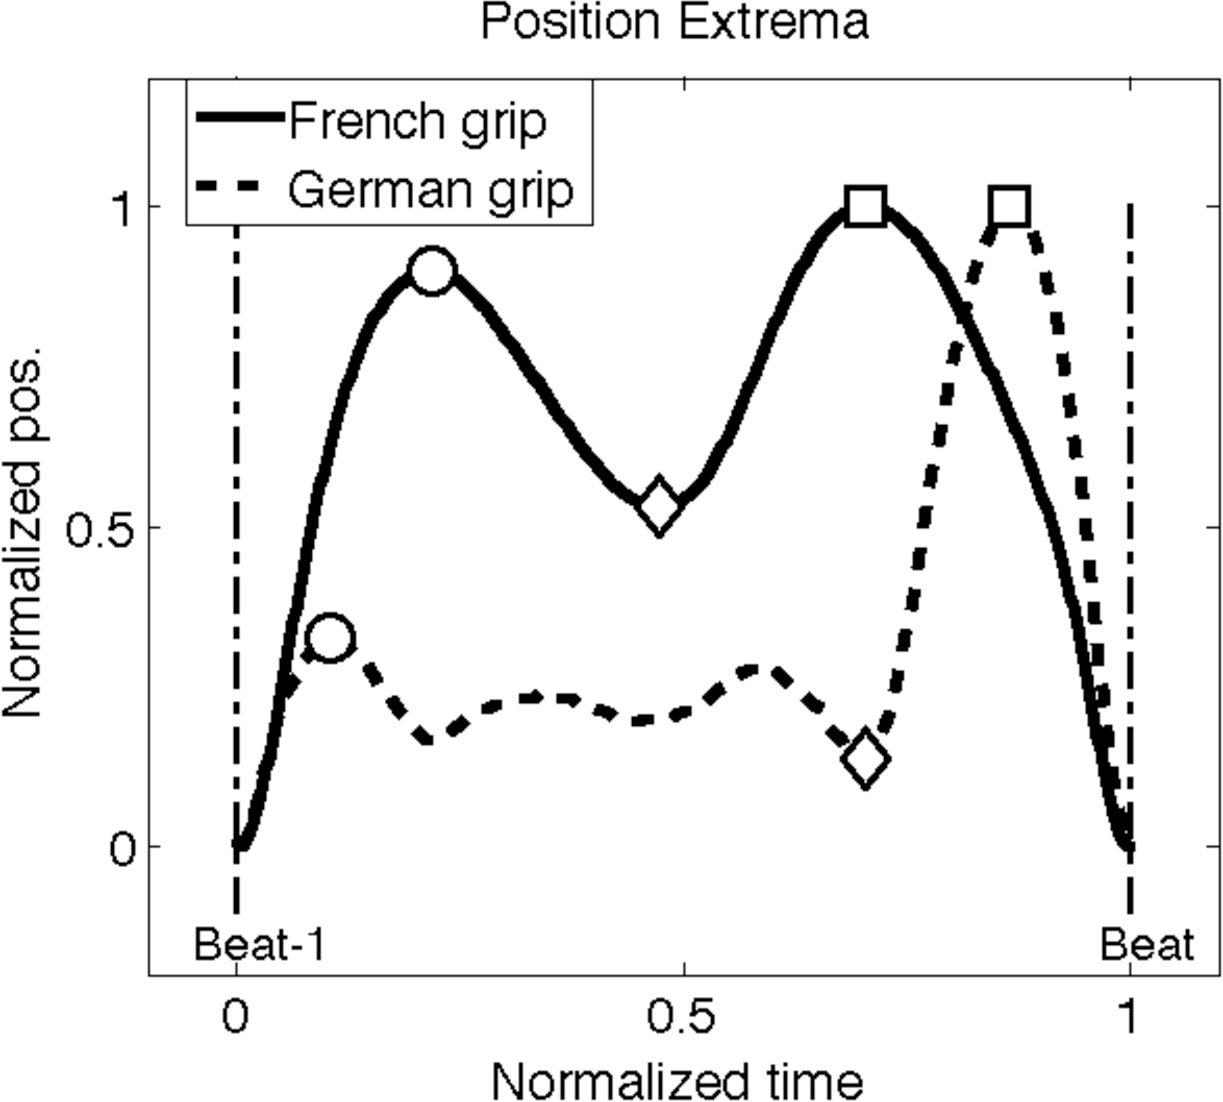
\includegraphics[width=0.45\linewidth]{Chapters/4/Pics/Pdf/GripsProfiles_Normalized2.pdf}}
%		\hspace{6mm}
%		\subfigure[]{\label{fig:classifParameters2}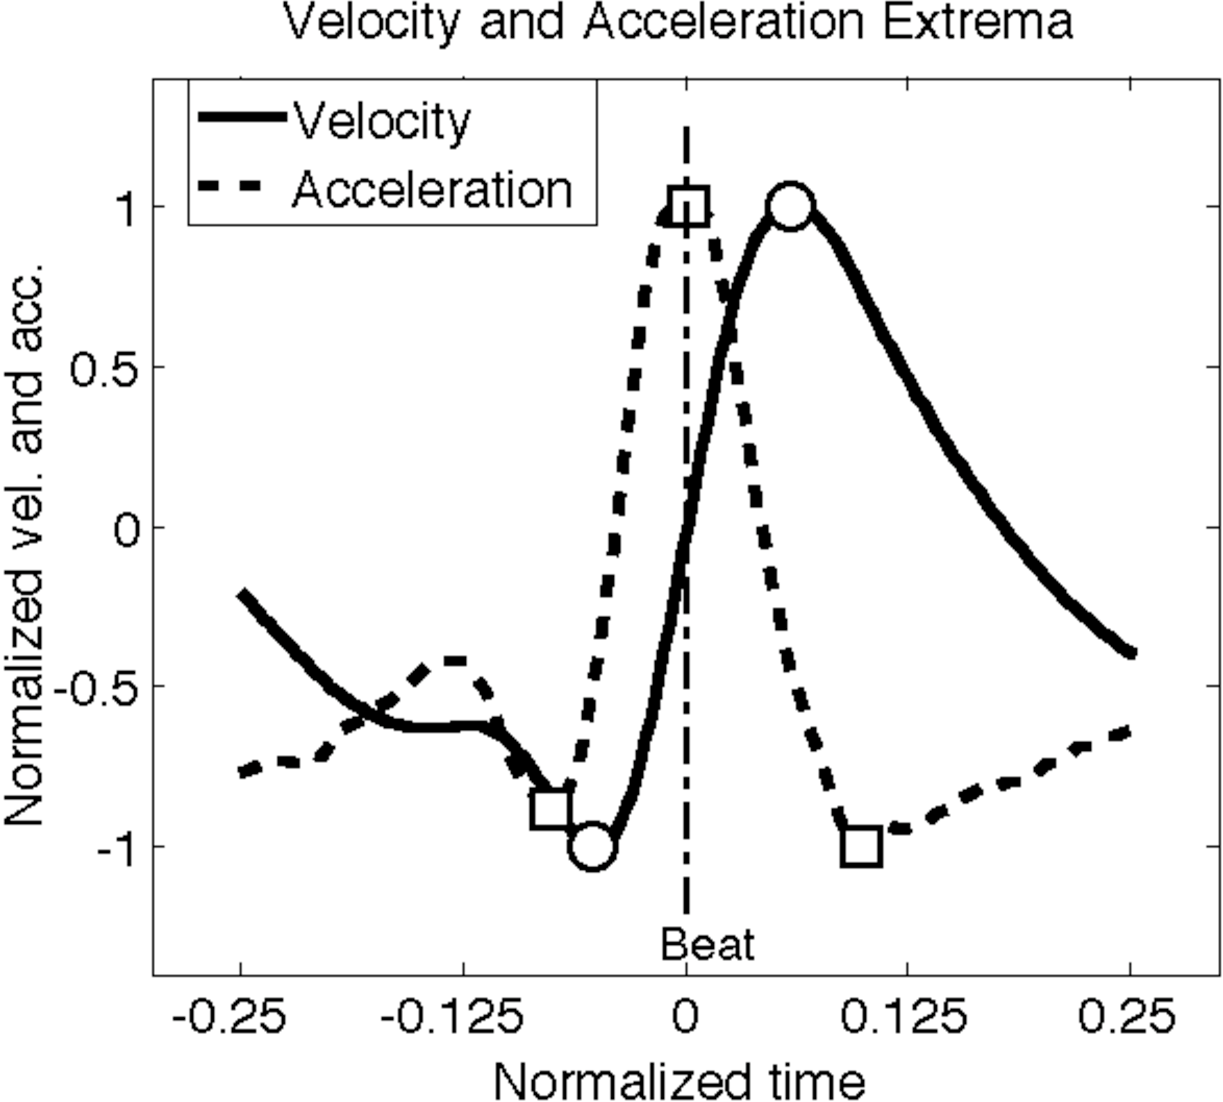
\includegraphics[width=0.45\linewidth]{Chapters/4/Pics/Pdf/VelocityAccelerationProfiles_Normalized2.pdf}}
		\subfigure[]{\label{fig:classifParameters1}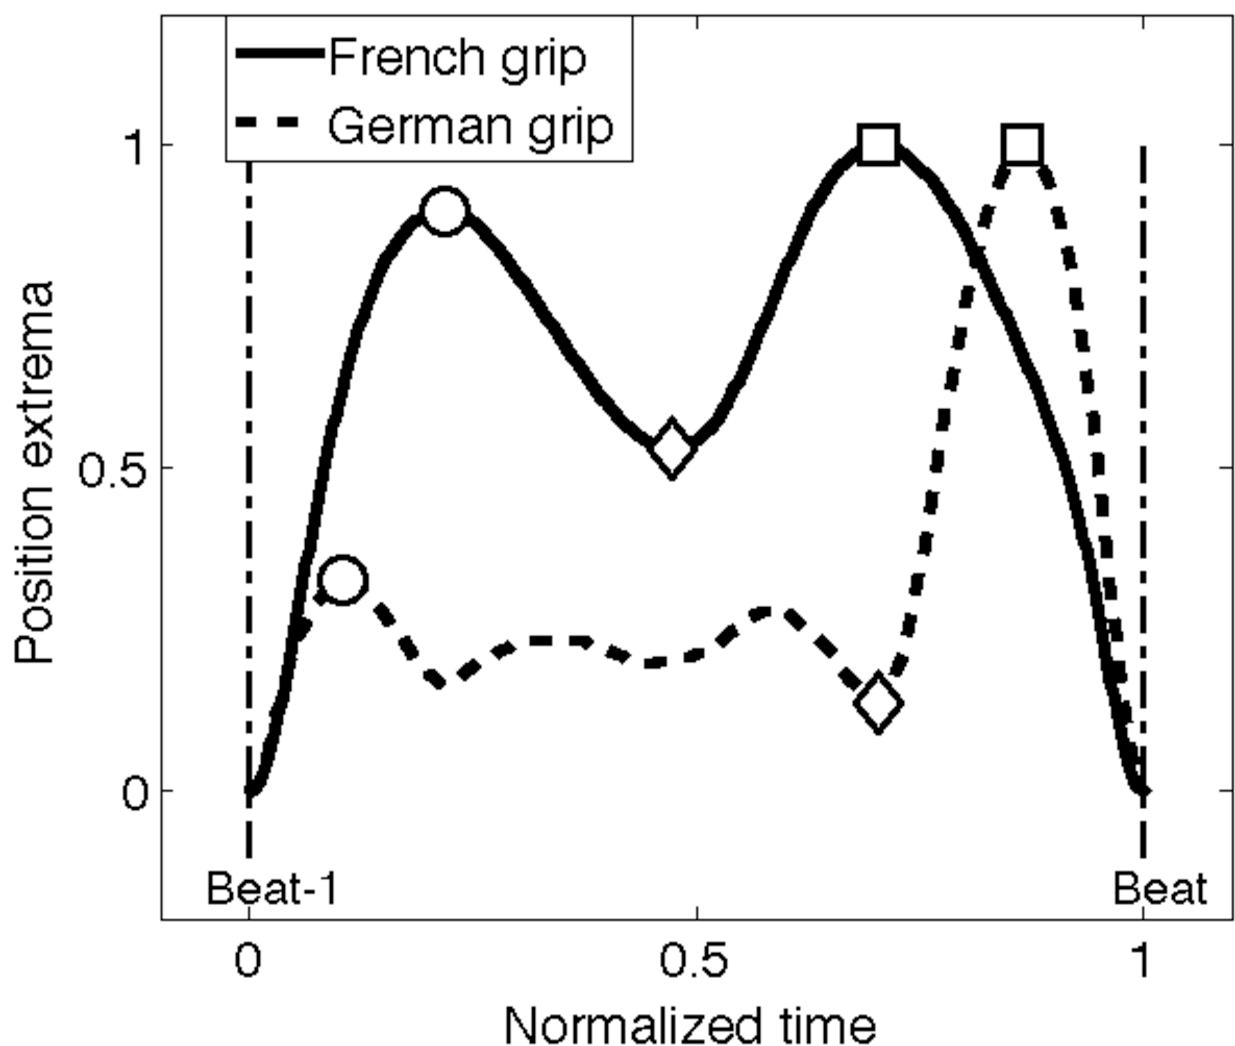
\includegraphics[width=0.45\linewidth]{Chapters/4/Pics/Pdf/pos_parameters.pdf}}
		\hspace{6mm}
		\subfigure[]{\label{fig:classifParameters2}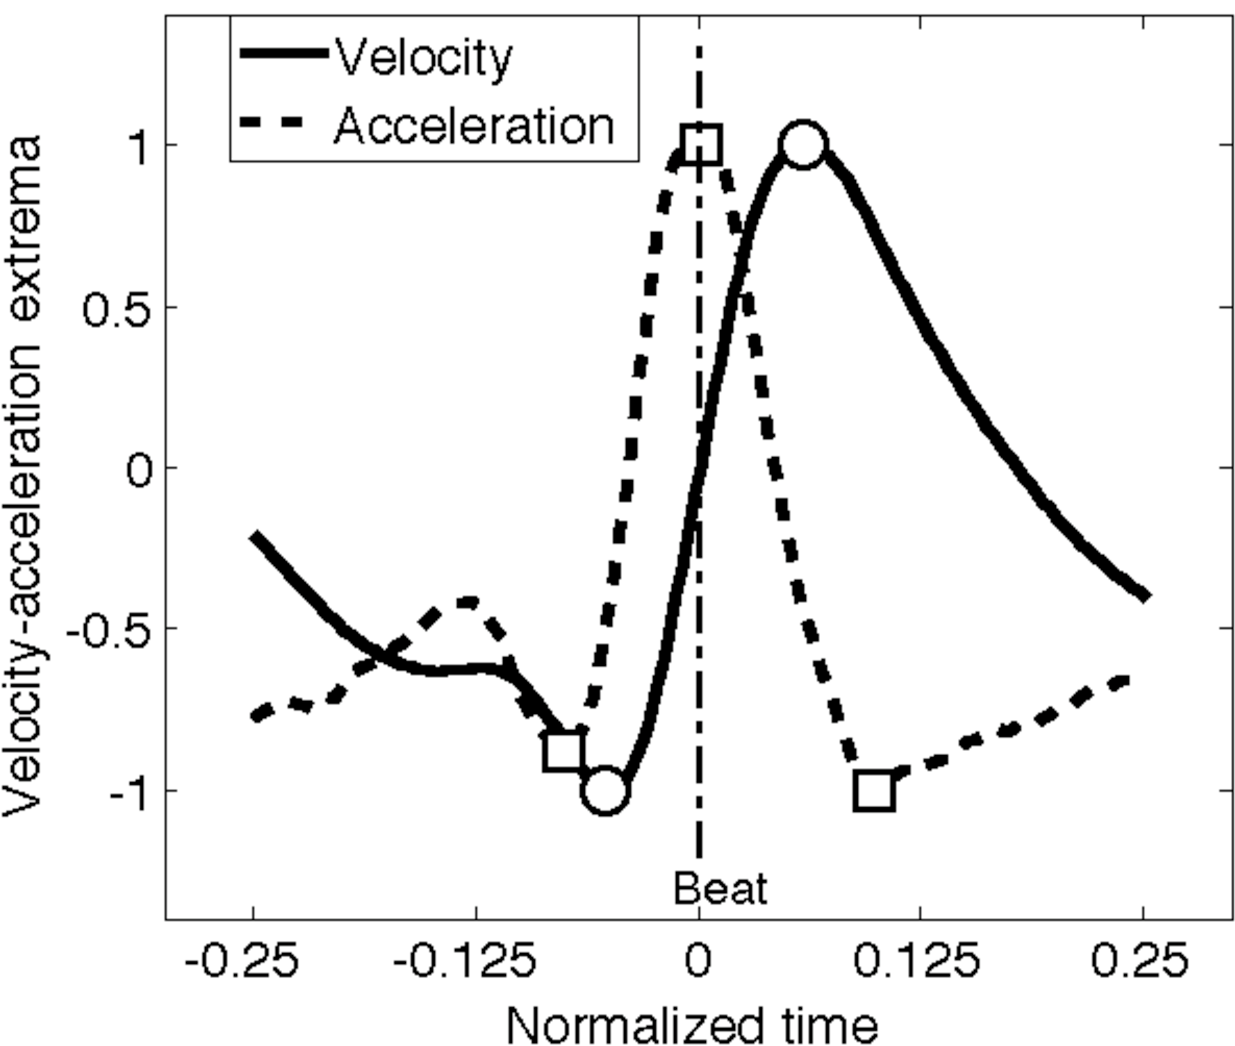
\includegraphics[width=0.45\linewidth]{Chapters/4/Pics/Pdf/vel_acc_parameters.pdf}}
	\end{center}
	\vspace{-0.5cm}
	\caption[Characterization of timpani playing techniques]{Extrema parameters used in the classification/recognition process for characterizing percussion gestures, extracted from: (a) mallet height position during \emph{beat-to-beat preparatory} phases (marker typology: $E_1$ = $\bigcirc$, $E_2$ = $\Diamond$ and $E_3$ = $\square$) and (b) velocity and acceleration \emph{beat-centered} profiles. These parameters are normalized for display purposes.}
	\label{fig:classifParameters}
\end{figure}

\begin{figure}%[H]
	\begin{center}
		\subfigure[]{\label{fig:profiles1}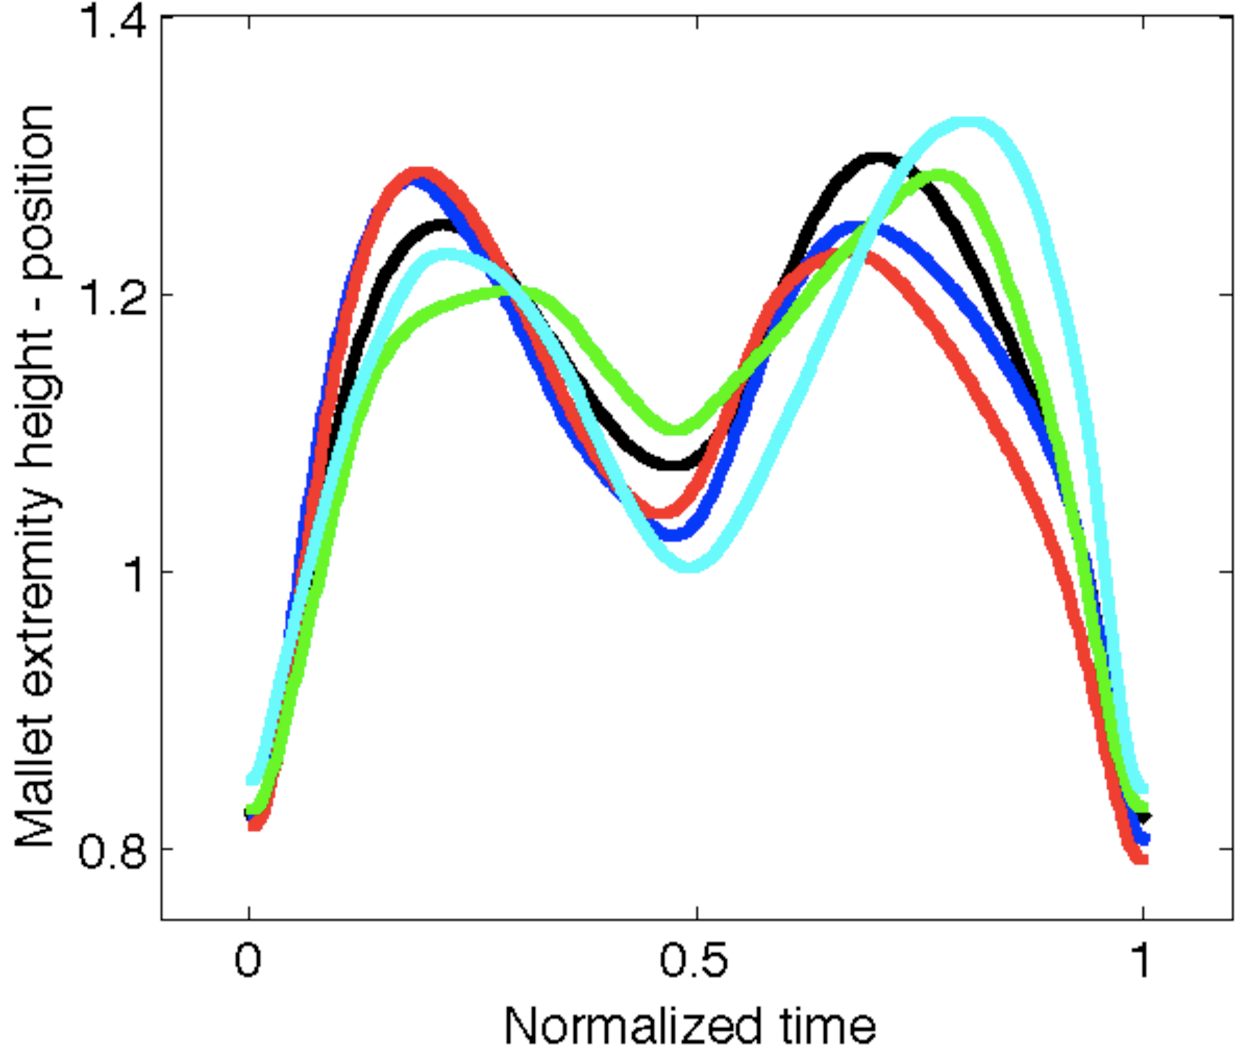
\includegraphics[width=0.45\linewidth]{Chapters/4/Pics/Pdf/french_position.pdf}}
		\hspace{6mm}
		\subfigure[]{\label{fig:profiles2}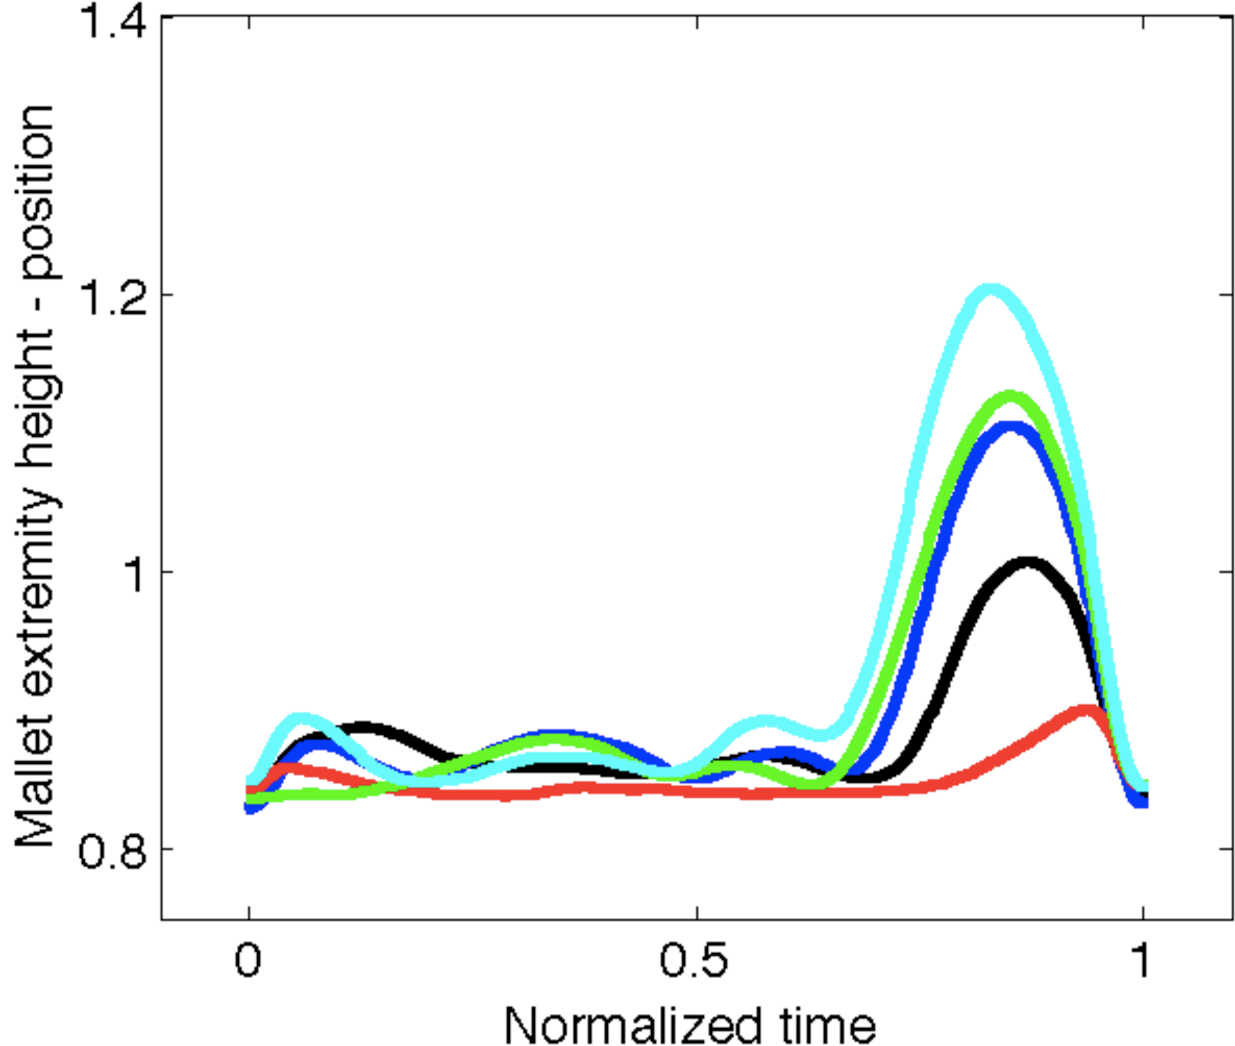
\includegraphics[width=0.45\linewidth]{Chapters/4/Pics/Pdf/german_position.pdf}}\\
		\subfigure[]{\label{fig:profiles3}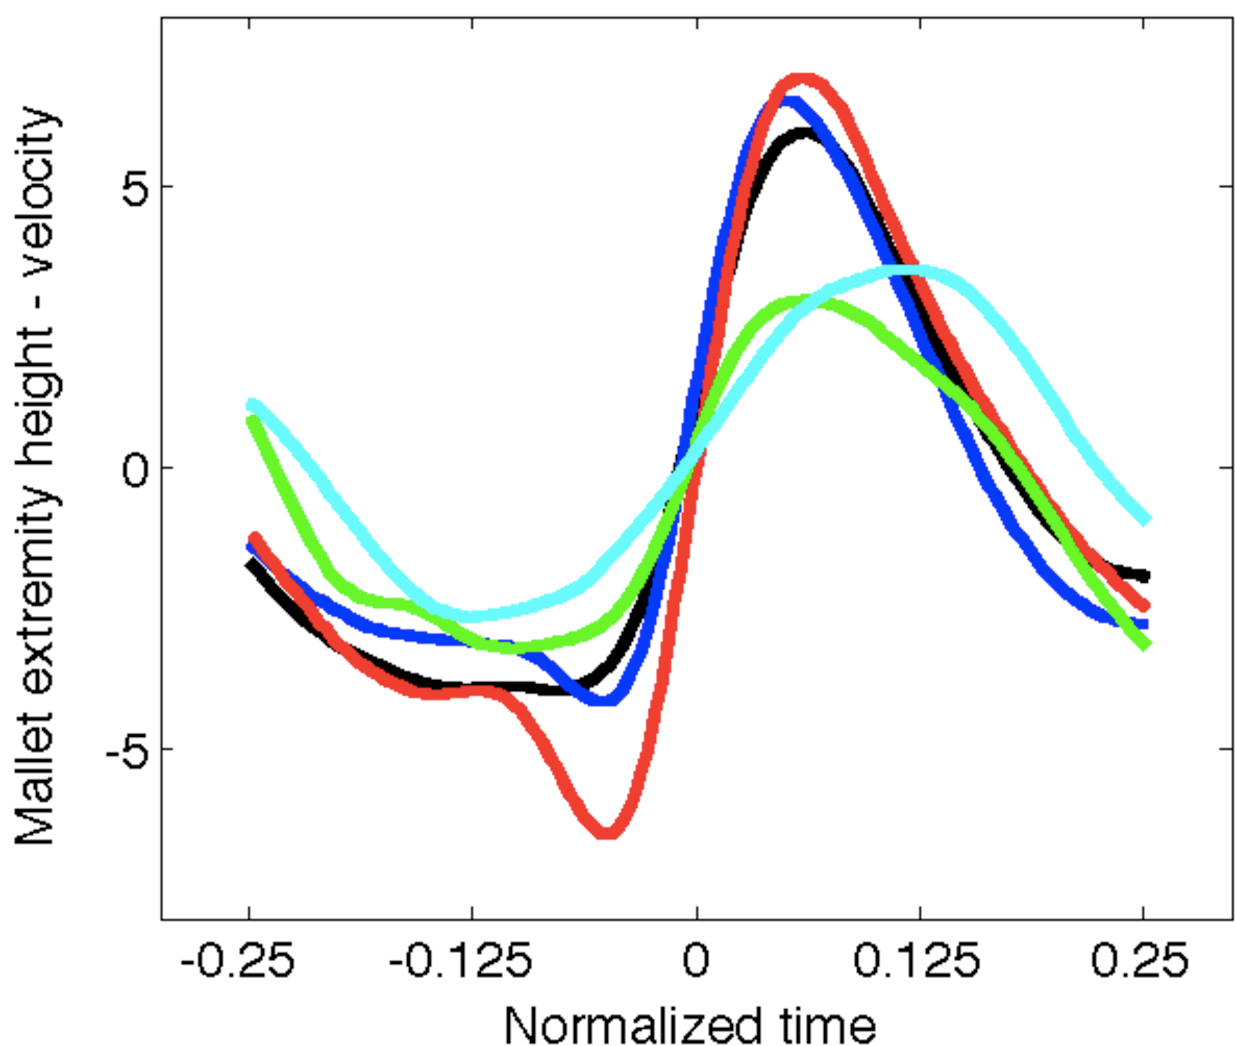
\includegraphics[width=0.45\linewidth]{Chapters/4/Pics/Pdf/french_velocity.pdf}}
		\hspace{6mm}
		\subfigure[]{\label{fig:profiles4}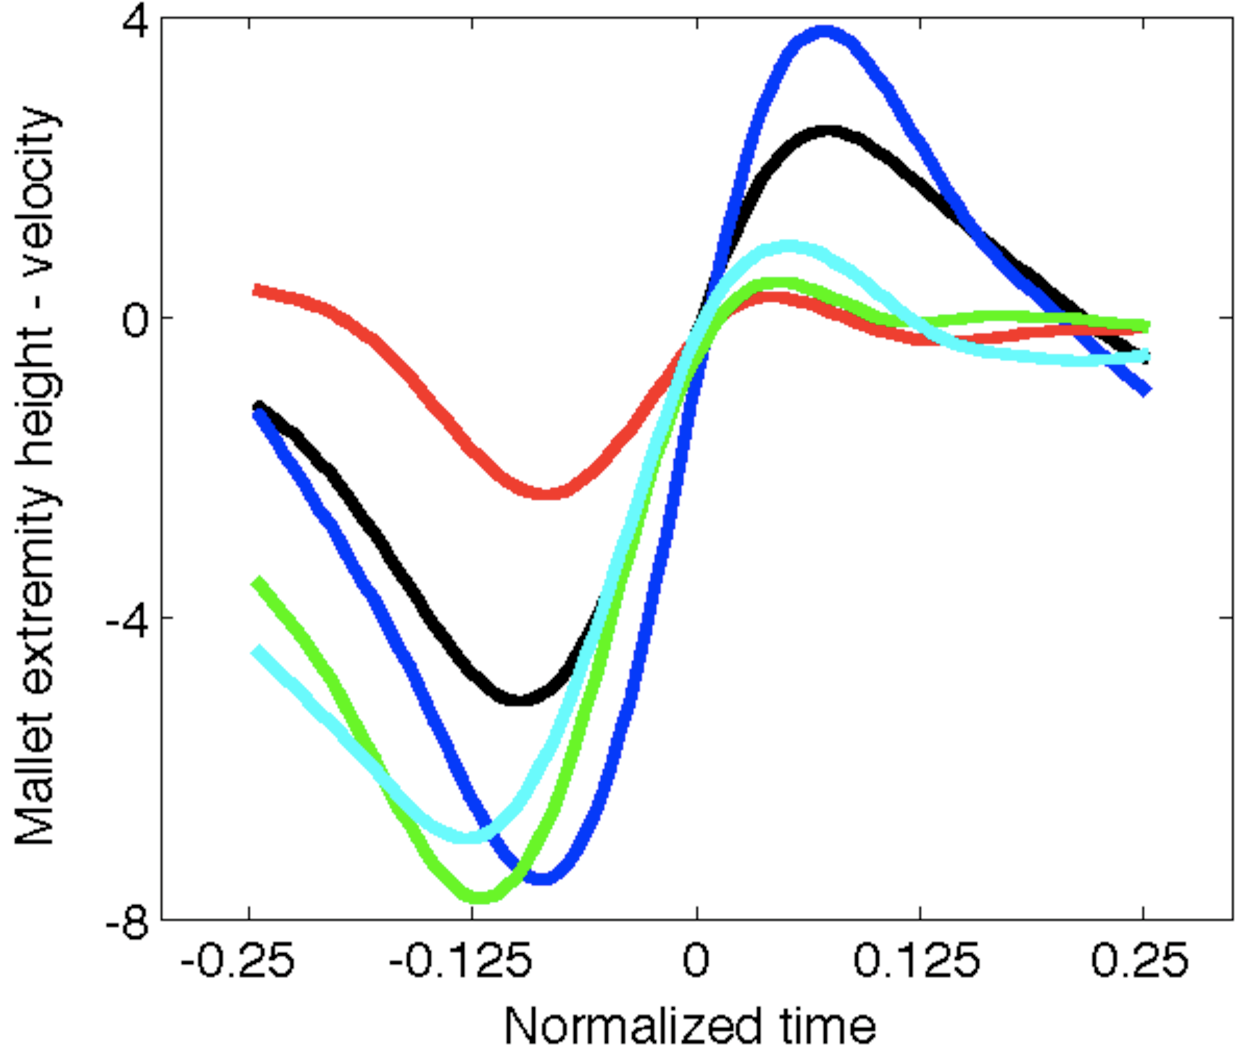
\includegraphics[width=0.45\linewidth]{Chapters/4/Pics/Pdf/german_velocity.pdf}}\\
		\subfigure[]{\label{fig:profiles5}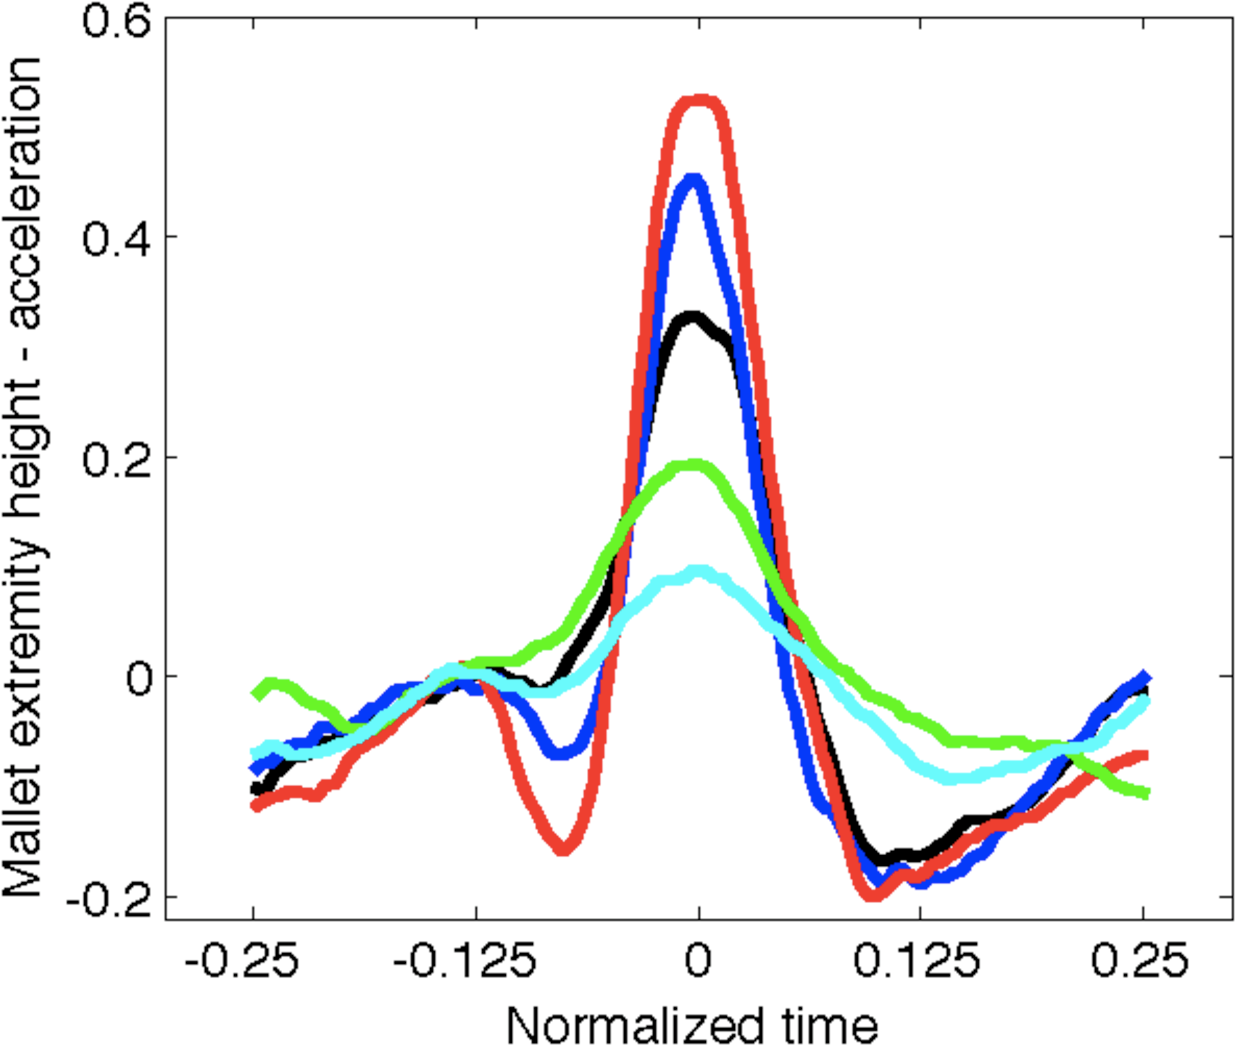
\includegraphics[width=0.45\linewidth]{Chapters/4/Pics/Pdf/french_acceleration.pdf}}
		\hspace{6mm}
		\subfigure[]{\label{fig:profiles6}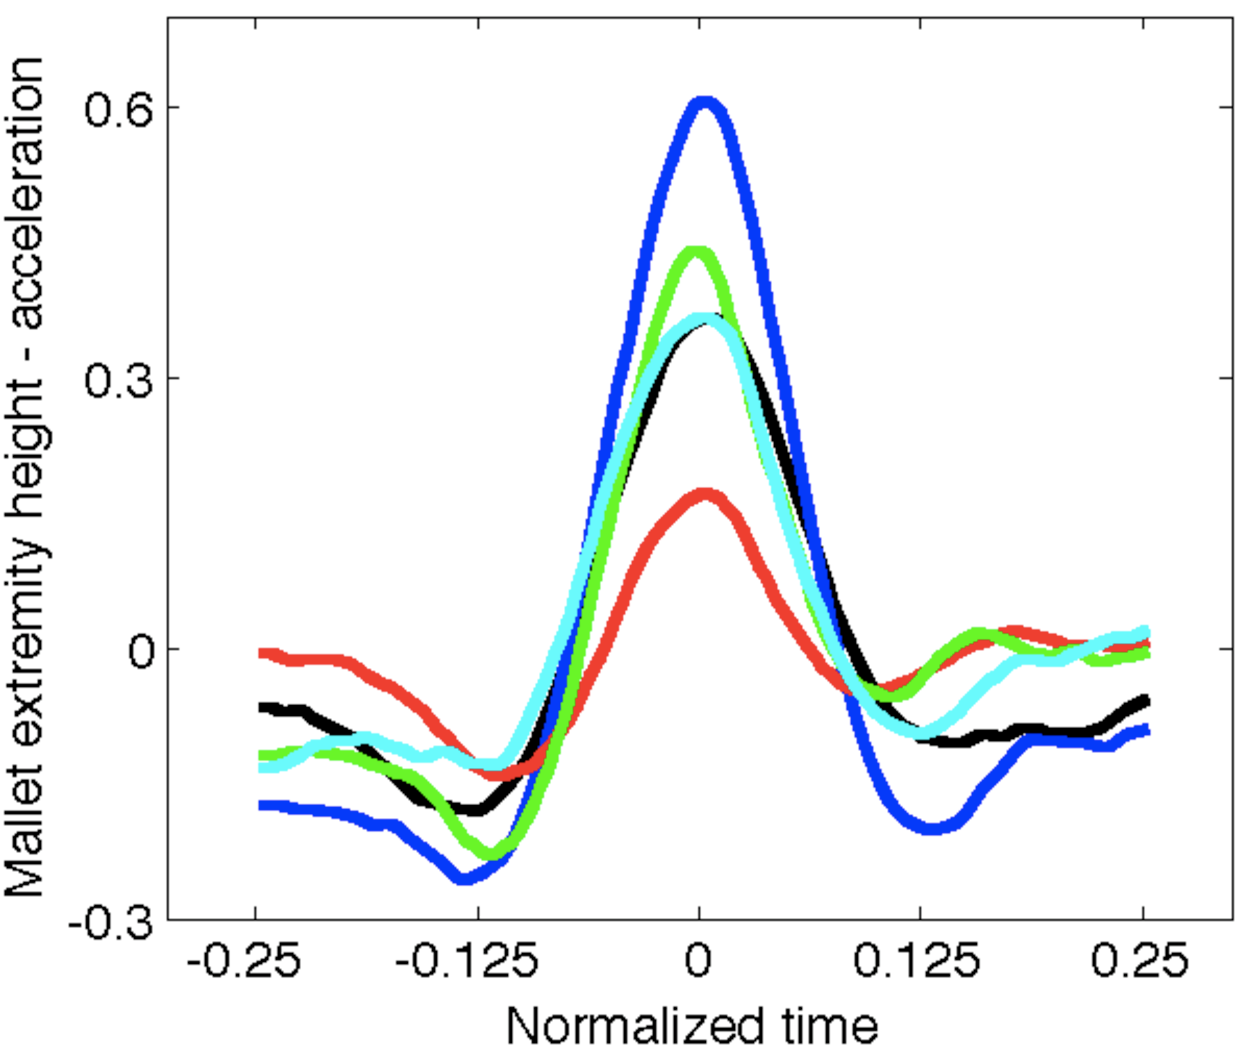
\includegraphics[width=0.45\linewidth]{Chapters/4/Pics/Pdf/german_acceleration.pdf}}
	\end{center}
	\vspace{-0.5cm}
	\caption[Position, velocity and acceleration profiles]{Position, velocity and acceleration profiles, respectively (a), (c) and (e) for the \emph{French} grip, and (b), (d), (f) for the \emph{German} grip.}
	\label{fig:profiles}
\end{figure}


		\subsection{Percussion Grips}
		\label{subsec:Analysis_TimpaniAnalysis_Grips}

First of all, we focus on the analysis of the influence of \emph{French} and \emph{German} grips on mallet trajectories. Quantitative features (\mytabname \ref{tab:statsTip}) processed on the vertical component of the tip of the mallet show that \emph{French} grip-related data performs the same timpani gesture with much more amplitude. The mean of the mallet extremity height is about twenty centimeters higher than its \emph{German} grip counterpart, with a variance twice higher. This fact is strengthened by the vertical range of motion ($RoM$) of the tip of the stick for \emph{French} grip-related data that is about twice higher than for \emph{German} grip data. The mean of mallet extremity height for \emph{German} grip data shows moreover that the tip of the stick is in average closer to the timpani membrane.\\

Specific local extrema can also be observed during the preparatory gesture of beat attacks. \myfigname \ref{fig:classifParameters} presents an example of the vertical component of the preparatory gesture between two beat attacks, and the identification of three characteristic extrema denoted $E_1$, $E_2$ and $E_3$. These extrema are temporally (temporal apparition in percentage of gesture's duration) and spatially characterized in \mytabname \ref{tab:statsTip}.

\begin{table}%[H]
	\centering
	\caption[Mallet trajectories and extracted extrema: statistical features]{Statistical features computed on mallet trajectories and extracted extrema: vertical Mean ($M$), Variance ($Var$) and Range of Motion ($RoM$), as well as the average temporal (in percentage of gesture's duration) and spatial characterization of extracted extrema presented in \myfigname \ref{fig:classifParameters}.}
	\vspace{2mm}
	\begin{tabular}{||x{1.6cm}||x{1.55cm}|x{1.55cm}|x{1.55cm}||x{1.6cm}|x{1.6cm}|x{1.6cm}||} \hline
		\small{$Stats$ / $Grips$} &	\small{$M$} \scriptsize{$[m]$} & 	\small{$Var$} \scriptsize{$[m]$} &	\small{$RoM$} \scriptsize{$[m]$} &	\small{$E_1$} \scriptsize{$[\% / m]$} &	\small{$E_2$} \scriptsize{$[\% / m]$} &	\small{$E_3$} \scriptsize{$[\% / m]$} 			\tabularnewline  \hline \hline
		\small{$French$} &	\small{1.1} &	\small{0.1} &	\small{0.04} &	\small{0.21 / 1.3} &	\small{0.47 / 1.1} &	\small{0.68 / 1.3}	\tabularnewline \hline
		\small{$German$} &	\small{0.9} &	\small{0.05} &	\small{0.02} &	\small{0.12 / 0.9} & 	\small{0.68 / 0.8} &	\small{0.85 / 1.0}		\tabularnewline \hline
	\end{tabular}
	\label{tab:statsTip}
\end{table}

Vertical extrema $E_1$, $E_2$ and $E_3$ are temporally equi-distributed for the \emph{French} grip-related data showing a continuous preparatory gesture, whereas local extrema for \emph{German} grip-related data denote three discontinuous parts. In this latter case, $E_1$ corresponds to the reaction to the previous beat attack, between $E_1$ and $E_2$ the tip of the mallet seems to seek a rest position (during more than the half of the whole movement duration) just above the timpani membrane, while $E_2$ and $E_3$ correspond to the amplitude that \emph{German} grip-related data gives for the following beat attack. \mytabname \ref{tab:statsTip} quantifies also the effect of the \emph{French} and \emph{German} grips on the vertical amplitude of the extrema.\\

\emph{French} and \emph{German} grips influence the spatial and temporal characteristics of the extracted extrema from height trajectories of the tip of the mallets. For evaluating the relevance of such parameters to distinguish these percussion grips, we chose to use a classification/recognition process. The training set is randomly composed of only 1/8$^{th}$ of the total number of available data, and the query set is composed of the remaining data.\\

\begin{table}%[H]
	\centering
	\caption[SVM recognition of timpani grips]{SVM recognition of timpani grips (in percentage of success) using the mallet position extrema presented in \myfigname \ref{fig:classifParameters}.}
	\vspace{2mm}
	\begin{tabular}{||x{1.9cm}||x{1.9cm}|x{1.9cm}||} \hline
		\small{$Training$ / $Test$} & 	\small{$French$} & 		\small{$German$}	\tabularnewline \hline \hline 
		\small{$French$} & 				\small{\textbf{98.2}} & \small{1.8}				\tabularnewline \hline
		\small{$German$} & 				\small{2.7} & 			\small{\textbf{97.3}}	\tabularnewline \hline
	\end{tabular}
	\label{tab:recognitionGrips}
\end{table}

\begin{table}%[H]
	\centering
	\caption[SVM recognition of \emph{French} grip playing modes]{SVM recognition of $French$ grip playing modes (in percentage of success) using the combination of mallet velocity and acceleration extrema presented in \myfigname \ref{fig:classifParameters}.}
	\vspace{2mm}
	\begin{tabular}{||x{1.9cm}||x{1.9cm}|x{1.9cm}|x{1.9cm}|x{1.9cm}|x{1.9cm}||} \hline
		\small{$Training$ / $Test$} & 	\small{$Legato$} &	\small{$Tenuto$} &	\small{$Accent$} &	\small{$V.\ Accent$} &	\small{$Staccato$}\tabularnewline \hline \hline
		\small{$Legato$} & 				\small{\textbf{96.2}} & \small{3.1} & \small{0} & \small{0.7} & \small{0}	\tabularnewline \hline
		\small{$Tenuto$} & 				\small{2.1} & \small{\textbf{92.6}} & \small{3.2} & \small{2.1} & \small{0}	\tabularnewline \hline
		\small{$Accent$} & 				\small{2.4} & \small{0} & \small{\textbf{94.7}} & \small{2.9} & \small{0}	\tabularnewline \hline
		\small{$V.\ Accent$} & 			\small{0} & \small{0} & \small{0} & \small{\textbf{93.4}} & \small{6.6}		\tabularnewline \hline
		\small{$Staccato$} & 			\small{0} & \small{0} & \small{0} & \small{3.3} & \small{\textbf{96.7}}		\tabularnewline \hline
	\end{tabular}
	\label{tab:recognitionFrenchVariations}
\end{table}

\begin{table}%[H]
	\centering
	\caption[SVM recognition of \emph{German} grip playing modes]{SVM recognition of $German$ grip playing modes (in percentage of success) using the combination of mallet position and acceleration extrema presented in \myfigname \ref{fig:classifParameters}.}
	\vspace{2mm}
	\begin{tabular}{||x{1.9cm}||x{1.9cm}|x{1.9cm}|x{1.9cm}|x{1.9cm}|x{1.9cm}||} \hline
		\small{$Training$ / $Test$} & 	\small{$Legato$} & 	\small{$Tenuto$} & 	\small{$Accent$} & 	\small{$V.\ Accent$} & 	\small{$Staccato$}\tabularnewline \hline \hline
		\small{$Legato$} & 				\small{\textbf{92.4}} &	\small{5.1} & \small{0} & \small{2.5} &	\small{0}	\tabularnewline \hline
		\small{$Tenuto$} & 				\small{3.3} & \small{\textbf{93.1}} & \small{0} & \small{1.1} &	\small{2.5}	\tabularnewline \hline
		\small{$Accent$} & 				\small{2.9} & \small{0} & \small{\textbf{94.3}} & \small{2.8} & \small{0}	\tabularnewline \hline
		\small{$V.\ Accent$} & 			\small{1.7} & \small{0} & \small{1.6} & \small{\textbf{91.8}} & \small{4.9}	\tabularnewline \hline
		\small{$Staccato$} & 			\small{1.1} & \small{0} & \small{0} & \small{5.4} & \small{\textbf{93.5}}	\tabularnewline \hline
	\end{tabular}
	\label{tab:recognitionGermanVariations}
\end{table}

The high recognition rates of these extrema (superior to 97{\%} in average), as shown by the confusion matrix in \mytabname \ref{tab:recognitionGrips}, indicate that such a parameterization is well-suited for characterizing the effect of percussion grips on the height trajectories of mallets.
 
 
		\subsection{Playing Modes}
		\label{subsec:Analysis_TimpaniAnalysis_Gestures}

Following the same methodology, the considered set of extracted parameters is enhanced for taking into account more timpani playing techniques, namely the different playing modes available in the motion capture database (\emph{legato}, \emph{tenuto}, \emph{accent}, \emph{vertical accent} and \emph{staccato}) for each percussion grip sub-group. These additionnal parameters are composed of the previously presented mallet height extrema (\myfigname \ref{fig:classifParameters1}), as well as local extrema extracted from mallet height velocity and acceleration on \emph{beat-centered} profiles (\myfigname \ref{fig:classifParameters2}). Beat-centered profiles are the truncation of motion to a window of $120$ milli-second, $60$ milli-second before and after the beat impact occurs.\\

In both situations for classifying playing modes inside percussion grips, the training set is randomly composed of only 1/4$^{th}$ of the total number of available data, and the query set is composed of the remaining data.\\ 

The classification of playing modes related to the \emph{French} grip is achieved by considering the combination of $velocity$ and $acceleration$ extrema. The results obtained with such a parameterization are presented by the confusion matrix in \mytabname \ref{tab:recognitionFrenchVariations}, with an average recognition rate superior to 94{\%}.\\

Concerning playing modes related to the \emph{German} grip, the classification is achieved by combining both $position$ and $acceleration$ extrema. The results obtained with such a parameterization are presented by the confusion matrix in \mytabname \ref{tab:recognitionGermanVariations}, whith an average recognition rate superior to 93{\%}.


		\subsection{Discussion}
		\label{subsec:Analysis_Discussion}

We discuss in this subsection both the nature of the parameters extracted for separating grips and playing modes, as well as the classification technique used for obtaining such results.


			\subsubsection{Nature of the Parameters}
			\label{subsubsec:Analysis_Discussion_Parameters}
			
Regarding the nature of the spatio-temporal parameters highlighted through this analysis, we think that they are relevant according to the percussion task, since both the height and the timing of gestures are highly controlled during percussion performances. The introduction of velocity and acceleration characteristics for discriminating between playing modes among \emph{French} and \emph{German} grips-related data can be interpreted as the parameterization of the dynamics intrinsically related to each playing mode.\\

More interesting is the use of different parameters' combinations ($velocity/ \\ acceleration$ for \emph{French} grip playing modes, and $position/acceleration$ for \emph{German} grip playing modes). This is to be related to the statistical features presented in subsection \ref{subsec:Analysis_TimpaniAnalysis_Grips}.

\mytabname \ref{tab:statsTip} shows indeed a mallet range of motion much more constrained for the \emph{German} grip, attesting the importance of position parameters for discriminating playing modes in this case. On the contrary, the continuous and equi-distributed preparatory gesture shown for the \emph{French} grip underlines a less stiff constraint on mallet position, so that the way velocity is involved is preponderant for discriminating playing modes in this particular situation. Acceleration parameters are both grip playing modes important features, as they may be related to the effort of the strike.


			\subsubsection{Classification Technique}
			\label{subsubsec:Analysis_Discussion_Classification}

Another issue to be discussed about the results presented in this chapter is the classification technique used in the methodology of our work. The classification/recognition technique chosen in this work is the \emph{SVM} method with \emph{RBF} kernel functions. The reason of this choice is that the \emph{SVM} technique gives really good results in the discrimination of mallet grips and playing modes. As an illustration of this affirmation, we have conducted the same classification/recognition methodology as presented in subsection \ref{subsec:Analysis_TimpaniAnalysis_Methodo} with replacing the \emph{SVM} technique by the K-Nearer-Neighbours (\emph{KNN}) method. \mytabname \ref{tab:recognitionGripsKNN}, \ref{tab:recognitionFrenchVariationsKNN} and \ref{tab:recognitionGermanVariationsKNN} respectively show the recognition results for the mallet grips, the \emph{French} and \emph{German} playing modes when using the \emph{KNN} technique.\\

Apart from the results concerning the mallet grips, these results attest lower recognition results compared with the results obtained with the \emph{SVM} technique (\mytabname \ref{tab:recognitionGrips}, \ref{tab:recognitionFrenchVariations} and \ref{tab:recognitionGermanVariations}).

Although the explanation of this discrepancy in the recognition quality is out of the scope of our thesis work, a qualitative and intuitive analysis leads us to hypothetize that the classes to be classified and recognized in the case of mallet grips are linearly separable (high recognition rates with the \emph{KNN} technique), whereas those concerning playing modes are not (low recognition rates with the \emph{KNN} method).\\

Moreover, when detailing the applied methodology in this work, we have precised that we used \emph{RBF} kernel functions with their default parameters, so that no optimization process is involved in the recognition analysis developped in this work. We can therefore expect that an optimization process taking into account an identification of the \emph{RBF} kernel functions would lead to better results than those presented in \mytabname \ref{tab:recognitionGrips}, \ref{tab:recognitionFrenchVariations} and \ref{tab:recognitionGermanVariations}.

\begin{table}[H]
	\centering
	\caption[KNN recognition of timpani grips]{KNN recognition of timpani grips (in percentage of success) using the mallet position extrema presented in \myfigname \ref{fig:classifParameters}.}
	\vspace{2mm}
	\begin{tabular}{||x{1.9cm}||x{1.9cm}|x{1.9cm}||} \hline
		\small{$Training$ / $Test$} & 	\small{$French$} & 		\small{$German$}	\tabularnewline \hline \hline 
		\small{$French$} & 				\small{\textbf{96.4}} & \small{3.6}				\tabularnewline \hline
		\small{$German$} & 				\small{3.7} & 			\small{\textbf{96.3}}	\tabularnewline \hline
	\end{tabular}
	\label{tab:recognitionGripsKNN}
\end{table}

\begin{table}[H]
	\centering
	\caption[KNN recognition of \emph{French} grip playing modes]{KNN recognition of \emph{French} grip playing modes (in percentage of success) using the combination of mallet velocity and acceleration extrema presented in \myfigname \ref{fig:classifParameters}.}
	\vspace{2mm}
	\begin{tabular}{||x{1.9cm}||x{1.9cm}|x{1.9cm}|x{1.9cm}|x{1.9cm}|x{1.9cm}||} \hline
		\small{$Training$ / $Test$} & 	\small{$Legato$} &	\small{$Tenuto$} &	\small{$Accent$} &	\small{$V.\ Accent$} &	\small{$Staccato$}\tabularnewline \hline \hline
		\small{$Legato$} & 				\small{\textbf{65.5}} & \small{19.6} & \small{11} & \small{3.9} & \small{0}	\tabularnewline \hline
		\small{$Tenuto$} & 				\small{24.3} & \small{\textbf{59.3}} & \small{16.4} & \small{0} & \small{0}	\tabularnewline \hline
		\small{$Accent$} & 				\small{10.8} & \small{21.8} & \small{\textbf{67.4}} & \small{0} & \small{0}	\tabularnewline \hline
		\small{$V.\ Accent$} & 			\small{5.2} & \small{10.1} & \small{0} & \small{\textbf{65.5}} & \small{19.2}\tabularnewline \hline
		\small{$Staccato$} & 			\small{0.2} & \small{0} & \small{0} & \small{20.8} & \small{\textbf{69}}		\tabularnewline \hline
	\end{tabular}
	\label{tab:recognitionFrenchVariationsKNN}
\end{table}

\begin{table}[H]
	\centering
	\caption[KNN recognition of \emph{German} grip playing modes]{KNN recognition of \emph{German} grip playing modes (in percentage of success) using the combination of mallet position and acceleration extrema presented in \myfigname \ref{fig:classifParameters}.}
	\vspace{2mm}
	\begin{tabular}{||x{1.9cm}||x{1.9cm}|x{1.9cm}|x{1.9cm}|x{1.9cm}|x{1.9cm}||} \hline
		\small{$Training$ / $Test$} & 	\small{$Legato$} & 	\small{$Tenuto$} & 	\small{$Accent$} & 	\small{$V.\ Accent$} & 	\small{$Staccato$}\tabularnewline \hline \hline
		\small{$Legato$} & 				\small{\textbf{64.7}} &	\small{20} & \small{12.6} & \small{0.6} &	\small{2.1}	\tabularnewline \hline
		\small{$Tenuto$} & 				\small{14.9} & \small{\textbf{62.4}} & \small{16.1} & \small{1} &	\small{5.6}	\tabularnewline \hline
		\small{$Accent$} & 				\small{20.2} & \small{14.5} & \small{\textbf{60.7}} & \small{4.6} & \small{0}	\tabularnewline \hline
		\small{$V.\ Accent$} & 			\small{6.3} & \small{5.7} & \small{6.7} & \small{\textbf{61.9}} & \small{18.4}	\tabularnewline \hline
		\small{$Staccato$} & 			\small{5.1} & \small{6.5} & \small{0} & \small{23} & \small{\textbf{65.4}}	\tabularnewline \hline
	\end{tabular}
	\label{tab:recognitionGermanVariationsKNN}
\end{table}

%%%%%%%%%%%%%%%%%%%%%%%%%%%%%%%%%%%%%%%%%%%%%%%%%%%%%%%%%%%%%%%%%%%%%%%%%%%%%%%%%%%%%%%%%%%%%%%%%%%%%%%%%%%%%%%%%%%%


%%%%%%%%%%%%%%%%%%%%%%%%%%%%%%%%%%%%%%%%%%%%%%%%%%%%%%%%%%%%%%%%%%%%%%%%%%%%%%%%%%%%%%%%%%%%%%%%%%%%%%%%%%%%%%%%%%%%

%\newpage

	\section{Conclusion}
	\label{sec:Analysis_Conclusion}

In this chapter, we proposed a methodology for capturing and analysing timpani performances. It has led to the collection of motion capture data for several timpani performers, allowing the study of percussion playing percussion techniques such as mallet grips (\emph{French} and \emph{German}), various playing modes (\emph{legato}, \emph{tenuto}, \emph{accent}, \emph{vertical accent} and \emph{staccato}) as well as different beat impact locations (\emph{one-third}, \emph{center} and \emph{rim}).

This work specifically focused on percussion grips and playing modes, as a mean of justifying the interest and highlighting the importance of the control of mallet extremity trajectories during timpani performances. To that mean, the adopted analysis methodology has accomplished the evaluation of a parameterization of percussion playing techniques. The evaluation was conducted via the the discrimination success of playing techniques under study by training a classifier with the extracted parameters.

Both for the discrimination of percussion grips and playing modes, we presented the extraction of a set of parameters solely regarding mallet extremity trajectories. The evaluation of such a parameterization is proved to be consistent, as attested by the high recognition rates obtained trough this classification/recognition scheme.\\

%%%%%%%%%%%%%%%%%%%%%%%%%%%%%%%%%%%%%%%%%%%%%%%%%%%%%%%%%%%%%%%%%%%%%%%%%%%%%%%%%%%%%%%%%%%%%%%%%%%%%%%%%%%%%%%%%%%%


%\chapter{Hybrid Physics-based Motion Control}
%\markboth{Hybrid Physics-based Motion Control}{Hybrid Physics-based Motion Control}
\chapter{Synthesis of Timpani Percussion Performances}
\markboth{Synthesis of Timpani Percussion Performances}{Synthesis of Timpani Percussion Performances}
\label{chapter:Synthesis}


%%%%%%%%%%%%%%%%%%%%%%%%%%%%%%%%%%%%%%%%%%%%%%%%%%%%%%%%%%%%%%%%%%%%%%%%%%%%%%%%%%%%%%%%%%%%%%%%%%%%%%%%%%%%%%%%%%%%

%Playing a musical instrument involves complex human behaviours. While performing, a skilled musician is able to precisely control his motion and to perceive both the reaction of the instrument to his actions and the resulting sound. This relationship between performer actions and the effects on the produced sound is crucial for understanding the mechanisms underlying musical learning or performance. Transposing these real-world experiences into virtual environments provides the possibility to explore novel solutions for designing virtual characters interacting with virtual musical instruments, and by extension for designing animated entities interacting with objects producing realistic sounds.\\

In this chapter, we propose a physically-based framework, in which a virtual character dynamically interacts with a physically simulated percussive instrument\footnote{The results presented in this chapter are the basis of the simulation platform documented at \href{http://www-valoria.univ-ubs.fr/Alexandre.Bouenard/index.php/Research/PhDThesis}{http://www-valoria.univ-ubs.fr/Alexandre.Bouenard/index.php/Research/PhDThesis}}. In particular, we present and evaluate a novel motion control paradigm for controlling a physical model of a virtual character, which is consistent with the analysis work presented in the previous chapter. We also propose an interaction scheme for controlling sound synthesis processes from this physically-based simulation framework for synthesizing virtual percussion performances.\\

The chapter is organized as follows. %First we introduce the motivation of the need of a novel motion control paradigm for the targetted application that is to synthesize virtual percussion performances (section \ref{sec:Synthesis_Introduction}).
We present an overview of the physical mechanisms occuring in our framework during the synthesis of virtual percussion performance in section \ref{sec:Synthesis_Overview}. The physics kernel including the physics modeling of the virtual percussionist as well as the novel motion control paradigm is presented and evaluated in section \ref{sec:Synthesis_Physics}. Section \ref{sec:Synthesis_Control} addresses the control of sound synthesis processes by the physical simulation of the virtual percussionist. Finally, section \ref{sec:Synthesis_Conclusion} concludes this work on the synthesis of virtual percussion performances.

%%%%%%%%%%%%%%%%%%%%%%%%%%%%%%%%%%%%%%%%%%%%%%%%%%%%%%%%%%%%%%%%%%%%%%%%%%%%%%%%%%%%%%%%%%%%%%%%%%%%%%%%%%%%%%%%%%%%


%%%%%%%%%%%%%%%%%%%%%%%%%%%%%%%%%%%%%%%%%%%%%%%%%%%%%%%%%%%%%%%%%%%%%%%%%%%%%%%%%%%%%%%%%%%%%%%%%%%%%%%%%%%%%%%%%%%%

%\section{Introduction and Motivation}
%\label{sec:Synthesis_Introduction}

%Virtual characters playing virtual musical instruments must interact in real-time with the sounding environment. Dynamic simulation is a promising approach to finely represent and modulate this interaction. Moreover, captured human motion can provide a database covering a large variety of gestures with various levels of expressivity. Three main problems have to be addressed in animating characters performing percussion gestures. First, physically-based simulations driven by motion capture data have to be considered, so that the physical interaction with the virtual world can be taken into account, and the generated movements can be driven by real examples. A second critical issue is the sound synthesis techniques which have to be used so that an effective mapping can be implemented between parameters generated from motion and sound synthesis parameters. Finally, the synchronization of different modalities and its use in interactive applications needs to be considered.\\

%Controlling adaptative and responsive virtual characters has been intensively investigated in \emph{Computer Animation} research. Among controller-based methods, most of the contributions have addressed the control of articulated figures using robotics-inspired proportionnal derivative (\emph{PD}) controllers \citeCGA{raibert86}. This has inspired many works for handling different types of motor tasks such as walking, running \citeCGA{hodgins:SIGGRAPH95}, composing these tasks \citeCGA{faloutsos:SIGGRAPH01} and easying the hard and time-consuming process of tuning such \emph{PD} controllers \citeCGA{allen:SCA07}.

%More related to our work are hybrid methods combining physics-based controllers and kinematic motion data, which aim at associating the advantage of user controllability of kinematics methods and the responsiveness of dynamics controllers. Our work is based on the tracking of motion capture data but differs from previous works by having a fully dynamically controlled character. 

%The specificity of our contribution lies also in the integration and the possible collaboration between \emph{IK} and \emph{ID} controllers, rather than handling strategies for transtionning between kinematic and dynamic controllers \citeCGA{zordan:SCA02, shapiro:PG03, zordan:TOG05}. We can also find in \citeCGA{zordan:CAS99} the use of \emph{IK} as a pre-process for modifying the original captured motion and simulating it on a different character anthropometry, we rather use \emph{IK} as a basis of our hybrid control method for specifying the control of a dynamic character from end-effector trajectories. This hybrid collaboration is particularly consistent for the synthesis of such ballistic motion that is percussion performance, which is not taken into account in related contributions \citeCGA{zordan:CAS99} \citeCM{bouenard:NIME08}.\\

%Alongside to the dynamic animation of virtual characters, physics-based sound synthesis methods have been widely studied, with the analogous goal of creating adaptative sounds towards changes in environment or objects properties. Since the introduction into the graphics community of modeling the surface vibrations of objects for sound synthesis \citeCM{vanDenDoel:ICAD96}, most of works have either focused on the direct use of vibrational modes \citeCM{obrien:SCA02} based on measurements \citeCM{corbett:Presence07}, or the simulation of surface vibrations using the finite element method \citeCM{obrien:SIGGRAPH01}. More recently, the high interest on modal synthesis has led to acceleration algorithms for handling large and complex environments \citeCM{bonneel:TOG08}.

%Our work involves in a similar manner physical models based on modal synthesis, but we point out to the difficulty of relating these sound synthesis schemes to their cause in the context of music performance, i.e. the instrumental gesture of a virtual performer. Here the focus is on the simulation of instrumental (percussion) gestures, as well as on the mapping between motion and sound synthesis.\\

%We therefore propose an architecture for physically exploring the interaction between motion and sound synthesis that eases the synchronization of different modalities and heterogenous data types (motion capture, motion simulation, sound control parameters). Previous works also involved a motion-driven approach for the synchronized generation of soundtracks from animations \citeCM{takala:SIGGRAPH92}. But as recalled in \citeCM{vanDenDoel:SIGGRAPH01}, despite many recent improvements, most of computer animation and simulation frameworks are still reluctant to integrate such synchronization method, moving therefore away from the interactive realism and presence that sound can give to computer animation applications. Our goal is to show how a physics modeling of the motion-sound interaction, combined with a carefully-designed system architecture can be of interest to that mean. Such a contribution has been proposed for haptic rendering systems \citeCM{avanzini:CAVW06, sinclair:IC08}, but to our knowledge it has not yet been exploited for the simulation and interaction of instrumental gestures with physics-based sound synthesis.

%%%%%%%%%%%%%%%%%%%%%%%%%%%%%%%%%%%%%%%%%%%%%%%%%%%%%%%%%%%%%%%%%%%%%%%%%%%%%%%%%%%%%%%%%%%%%%%%%%%%%%%%%%%%%%%%%%%%


%%%%%%%%%%%%%%%%%%%%%%%%%%%%%%%%%%%%%%%%%%%%%%%%%%%%%%%%%%%%%%%%%%%%%%%%%%%%%%%%%%%%%%%%%%%%%%%%%%%%%%%%%%%%%%%%%%%%

	\section{Overview}
	\label{sec:Synthesis_Overview}

The architecture of our system is presented in \myfigname \ref{fig:overview} and is made of two modules, allowing the physics simulation of percussion gestures to control sound synthesis processes. The first module includes a motion capture database used for driving a motion control policy model of a physics-based character. The second module expresses the interaction between the percussion motion simulation and the physics-based sound synthesis.\\

Concerning the motion control, the specificity of our contribution lies in the integration and the possible collaboration between inverse kinematics (\emph{IK}) and inverse dynamics (\emph{ID}) controllers, rather than handling strategies for transtioning between kinematic and dynamic controllers \citeCGA{shapiro:PG03, mandel:MsC04, zordan:TOG05}. We can also find in \citeCGA{zordan:CAS99} the use of \emph{IK} as a pre-process for modifying the original captured motion and simulating it on a different character anthropometry. We rather use \emph{IK} as a basis of our hybrid control method for specifying the control of a dynamic character from end-effector trajectories. This hybrid collaboration is particularly consistent for the synthesis of such ballistic motion that is percussion performance, which is not taken into account in related contributions \citeCGA{zordan:CAS99} \citeCM{bouenard:NIME08}.\\

Concerning the sound synthesis, our work involves physical models based on modal synthesis in a similar manner to recent works \citeCGA{raghuvanshi:I3D06, bonneel:TOG08}. However we point out to the difficulty of relating these sound synthesis schemes to their cause in the context of music performance, i.e. the instrumental gesture of a virtual performer. Here the focus is on the simulation of instrumental (percussion) gestures, as well as on the interaction between motion and sound synthesis.\\

\begin{figure}%[H]
	\centering
	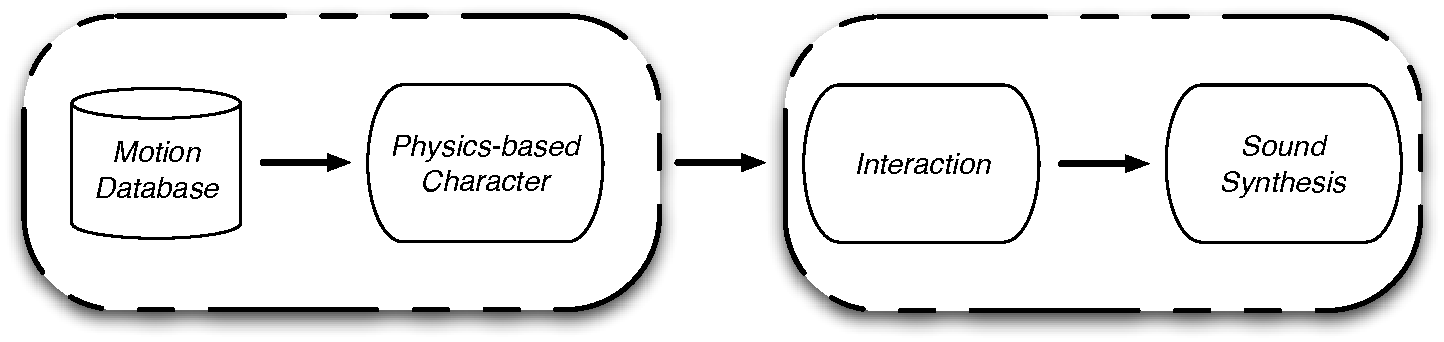
\includegraphics[width=0.9\linewidth]{Chapters/5/Pics/Pdf/overview3.pdf}
%	\vspace{-0.5cm}
	\caption[System architecture and multimodal outputs]{System architecture and multimodal outputs. The {\it Physics-based Motion Control and Synthesis} step involves a {\it Motion Capture Database} and results in the {\it Visual Feedback}. The {\it Interaction} expresses the mapping between the percussion motion simulation and the {\it Sound Synthesis}, which results in the {\it Sound Feedback}.}
	\label{fig:overview}
\end{figure}

In addition, we propose an architecture to allow the synchronization of different modalities and heterogenous data types (motion capture, motion simulation, sound control parameters), as well as to enable the users to explore various interaction schemes between motion and sound simulations. Previous works also involved a motion-driven approach for the synchronized generation of soundtracks from animations \citeCM{takala:SIGGRAPH92}. But as recalled in \citeCM{vanDenDoel:SIGGRAPH01}, despite many recent improvements, most of computer animation and simulation frameworks are still reluctant to integrate such synchronization method, moving therefore away from the interactive realism and presence that sound can give to computer animation applications. Our goal is to show how a physics modeling of the motion-sound interaction, combined with a carefully-designed system architecture can be of interest to that mean. Such a contribution has been proposed for haptic rendering systems \citeCM{avanzini:CAVW06, sinclair:IC08}, but to our knowledge it has not yet been exploited for the simulation and interaction of instrumental gestures with physics-based sound synthesis.

%The first module includes a motion capture database used for driving a physics-based model of a virtual percussionist ("Instrumental Gesture Simulation" module). Section \ref{sec:Synthesis_Physics} details the modeling of the virtual percusionist as well as the underlying motion control paradigms involved in our novel hybrid motion control scheme.

%The second module expresses the interaction between the percussion motion simulation and the sound synthesis model ("Interaction" module). Section \ref{sec:Synthesis_Control} details the specially designed architecture for accelerating and easying this process. We recall that our interest lies more in the control of a sound synthesis model by the parameters extracted from the physics simulation of the virtual performer than the sound synthesis itself. As an example, we give in this section a derivation of this control step in the case of a modal model of a drum membrane.

%The specificity of our contribution lies in the integration and the possible collaboration between \emph{IK} and \emph{ID} controllers, rather than handling strategies for transtionning between kinematic and dynamic controllers \citeCGA{shapiro:PG03, mandel:MsC04, zordan:TOG05}. We can also find in \citeCGA{zordan:CAS99} the use of \emph{IK} as a pre-process for modifying the original captured motion and simulating it on a different character anthropometry, we rather use \emph{IK} as a basis of our hybrid control method for specifying the control of a dynamic character from end-effector trajectories. This hybrid collaboration is particularly consistent for the synthesis of such ballistic motion that is percussion performance, which is not taken into account in related contributions \citeCGA{zordan:CAS99} \citeCM{bouenard:NIME08}.

%Our work involves physical models based on modal synthesis in a similar manner to recent works \citeCGA{raghuvanshi:I3D06, bonneel:TOG08}. However we point out to the difficulty of relating these sound synthesis schemes to their cause in the context of music performance, i.e. the instrumental gesture of a virtual performer. Here the focus is on the simulation of instrumental (percussion) gestures, as well as on the interaction between motion and sound synthesis.

%We therefore propose an architecture for physically exploring the interaction between motion and sound synthesis that eases the synchronization of different modalities and heterogenous data types (motion capture, motion simulation, sound control parameters). Previous works also involved a motion-driven approach for the synchronized generation of soundtracks from animations \citeCM{takala:SIGGRAPH92}. But as recalled in \citeCM{vanDenDoel:SIGGRAPH01}, despite many recent improvements, most of computer animation and simulation frameworks are still reluctant to integrate such synchronization method, moving therefore away from the interactive realism and presence that sound can give to computer animation applications. Our goal is to show how a physics modeling of the motion-sound interaction, combined with a carefully-designed system architecture can be of interest to that mean. Such a contribution has been proposed for haptic rendering systems \citeCM{avanzini:CAVW06, sinclair:IC08}, but to our knowledge it has not yet been exploited for the simulation and interaction of instrumental gestures with physics-based sound synthesis.\\

%The architecture of our system is presented in \myfigname \ref{fig:overview} and is made of two modules, allowing the physics simulation of percussion gestures to control sound synthesis processes.

%The first module includes a motion capture database used for driving a physics-based model of a virtual percussionist ("Instrumental Gesture Simulation" module). Section \ref{sec:Synthesis_Physics} details the modeling of the virtual percusionist as well as the underlying motion control paradigms involved in our novel hybrid motion control scheme.

%The second module expresses the interaction between the percussion motion simulation and the sound synthesis model ("Interaction" module). Section \ref{sec:Synthesis_Control} details the specially designed architecture for accelerating and easying this process. We recall that our interest lies more in the control of a sound synthesis model by the parameters extracted from the physics simulation of the virtual performer than the sound synthesis itself. As an example, we give in this section a derivation of this control step in the case of a modal model of a drum membrane.

%%%%%%%%%%%%%%%%%%%%%%%%%%%%%%%%%%%%%%%%%%%%%%%%%%%%%%%%%%%%%%%%%%%%%%%%%%%%%%%%%%%%%%%%%%%%%%%%%%%%%%%%%%%%%%%%%%%%


%%%%%%%%%%%%%%%%%%%%%%%%%%%%%%%%%%%%%%%%%%%%%%%%%%%%%%%%%%%%%%%%%%%%%%%%%%%%%%%%%%%%%%%%%%%%%%%%%%%%%%%%%%%%%%%%%%%%

	\section{Physics-based Modeling and Motion Control}
	\label{sec:Synthesis_Physics}

The approach that we adopt for physically controlling percussion gestures from motion capture data is described in \myfigname \ref{fig:modelControl}.\\

It involves the physical modeling of a musculo-skeleton virtual percussionist from pre-recorded percussion performances, by merging the two kinematics ($\boldsymbol{T^K}$, \myequname \eqref{eq:kinRepresentation}) and dynamics ($\boldsymbol{T^D}$, \myequname \eqref{eq:dynRepresentation}) representations presented in section \ref{subsec:CA_VCM}.\\

Our novel motion control paradigm takes advantage of this double and complementary representation by the definition of a sensorimotor controller that tracks motion capture data according to two control modes. The first control scheme uses simple \emph{ID} controllers similarly to previous contributions \citeCGA{raibert86, hodgins:SIGGRAPH95, zordan:SCA02}, whereas the second mode involves a novel hybrid motion control scheme including a cascaded process of \emph{IK} and \emph{ID} controllers. This latter allows the control of the physical model of a virtual percussionist solely by specifying mallet extremity trajectories ($\boldsymbol{X_t}$).

\begin{figure}%[H]
	\centering
	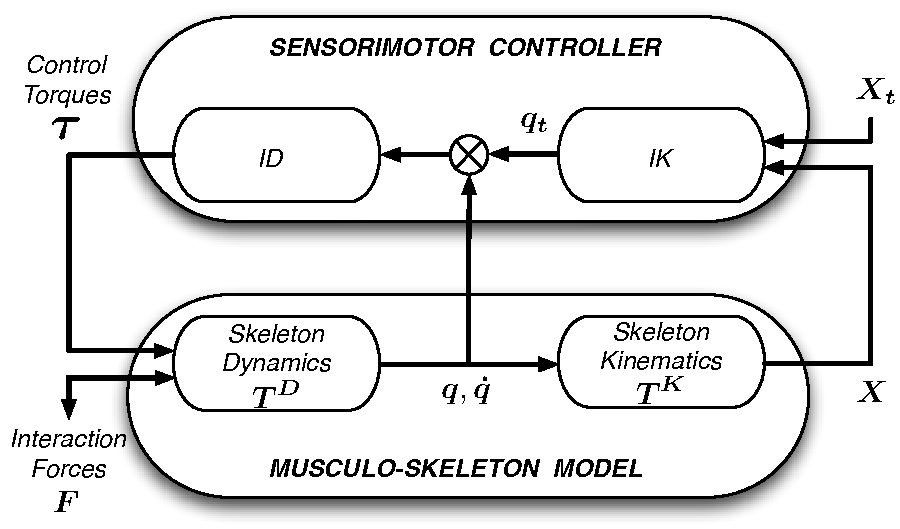
\includegraphics[width=0.7\linewidth]{Chapters/5/Pics/Pdf/IK-ID-Control.pdf}
%	\vspace{-0.5cm}
	\caption[Physics-based modeling and control]{Physics-based modeling and control.}
	\label{fig:modelControl}
\end{figure}


		\subsection{Virtual Character Modeling}
		\label{subsec:Synthesis_Physics_VirtualCharacterModeling}


			\subsubsection{Representation and Anthropometry}
			\label{subsubsec:Synthesis_Physics_VirtualCharacterModeling_RepAnt}

The musculo-skeleton model of the virtual performer is composed of two skeleton layers, a dynamics layer ($\boldsymbol{T^D}$) and a kinematics layer ($\boldsymbol{T^K}$). It should be noted that this representation is not generic to any human anthropometry but specific to the simplified anthropometry initially recorded (cf. section \ref{sec:Analysis_MoCapDatabase}).\\

The dynamics skeleton $\boldsymbol{T^D}$ models the physical properties of the virtual character, and is composed of rigid bodies articulated by mechanical joints. Motion capture data of percussion performances are used to physically model and parameterize both the anthropometry and the mechanical joints of the virtual character, making a direct correspondence between the real performer and the virtual character. The physical properties of each rigid body composing the virtual character, such as mass, size of the limbs, density and inertia matrix are consistent with the anthropometry extracted from motion capture data, by using anthropometric tables \citeCGA{dempster:AJA67}.\\

The kinematics layer $\boldsymbol{T^K}$ of the virtual performer is composed of kinematics linear-angular position and velocity ($\boldsymbol{q}$, $\boldsymbol{\dot{q}}$) of joints articulating the rigid body composing $\boldsymbol{T^D}$. State features $\boldsymbol{q}$ and $\boldsymbol{\dot{q}}$ are namely obtained by the integration of the motion equations over time (\myequname \eqref{eq:physNewtonFormulation} for instance).


			\subsubsection{Joints}
			\label{subsubsec:Synthesis_Physics_VirtualCharacterModeling_Joints}

In addition, each mechanical joint has three rotational degrees of freedom, restricted to the angular limits of the human body, in order to avoid non realistic motion. Two formulations are available to extract the "lower" and "upper" limits of the angular joints, based on a statistical analysis of the motion capture data.\\

The first formulation uses the Euler angles representation, and computes basic statistical features to characterize joint limits. The singularity of this represention is however frequent (\emph{gimbal lock}), therefore we propose another formulation based on the quaternionic representation.\\

Following the approach of \citeCGA{johnson:PhD03}, we compute joint limits in the quaternion space\footnote{Thanks go to the developpers of the SMR library from the \href{http://www-valoria.univ-ubs.fr/SAMSARA}{\emph{VALORIA-SAMSARA}} lab, and particularly to N. Courty for helpful hints about the quaternion representation.}. The rotational (quaternionic) trajectory $\boldsymbol{Q}$ of a joint over time is transposed in the tangential space of its quaternionic mean $\bar{q}$, in which an SVD decomposition is applied. The resulting eigen values and axes ($\boldsymbol{\lambda}$, $\boldsymbol{e}$) are used for representing the motion distribution and for computing the joint limits by the specification of a bounding ellipsoid (\myalgname \ref{alg:quatSVD}).

\begin{algorithm}
	%\dontprintsemicolon
	\emph{}\;

	\begin{center}
		\begin{tabular}[3cm]{rcc}
			\multirow{1}{*}{In} & $\boldsymbol{Q} = \lbrace q_i, i \in [[1 \dots n]]\rbrace$ & Quaternionic time serie \\
			\\
			\multirow{1}{*}{Out} & $\lbrace \boldsymbol{\lambda}, \boldsymbol{e} \rbrace$ & Eigen values and axes \\
		\end{tabular}
	\end{center}
	\emph{}\;

	\emph{** Mean of $Q$ **}\;
	$\bar{q}$ = mean($\boldsymbol{Q}$)\;
 	\emph{}\;
 	
	\emph{** Transposition of the motion $Q$ in the tangent space of $\bar{q}$ **}\;
	$\boldsymbol{Q^{*}} = \log(\bar{q}*\boldsymbol{Q})$\;
	\emph{}\;

	\emph{** Eigen values and axes **}\;
	$\lbrace \boldsymbol{\lambda}, \boldsymbol{e} \rbrace = SVD(\boldsymbol{Q^{*}})$\;
	\emph{}\;

	\caption{Formulating joint limits in the quaternion space}
	\label{alg:quatSVD}
\end{algorithm}


		\subsection{Motion Control}
		\label{subsec:Synthesis_Physics_MotionControl}

Our approach to dynamic character control uses percussion gestures from a motion capture database, allowing to take into account all the variability and expressiveness of real percussion gestures. The variability can be due to various percussion performances using different mallet grips, various beat impact locations and several musical playing modes (see section \ref{sec:Analysis_MoCapDatabase}).\\

We propose two ways for achieving the motion control of the musculo-skeleton model (see \myfigname \ref{fig:motionSynthesis}), either by tracking motion capture data in the joint space (angular trajectories), or a novel hybrid motion control scheme for tracking end-effector trajectories in the 3D cartesian space. Tracking motion capture data in joint space requires \emph{ID} control, whereas tracking in the end-effector space requires both a cascaded collaboration of \emph{IK} and \emph{ID} controllers. In this latter case, the two inversion processes are strongly linked. 


			\subsubsection{\emph{ID} Motion Control}
			\label{subsec:Synthesis_Physics_MotionControl_InverseDynamics}

This control mode is related to motion capture data tracking by using \emph{ID} controllers. Angular trajectories ($\boldsymbol{\Theta_t}$) are first extracted from motion capture data, and used to drive the fully dynamically controlled virtual character. We use traditional proportional-derivative feedback controllers, modeled as damped springs and parameterized by manually-tuned damping and stiffness coefficients ($k_d$, $k_s$). Knowing the current state of the mechanical joint ($\boldsymbol{q}$, $\dot{\boldsymbol{q}}$) and the joint target ($\boldsymbol{q_t}$) to be reached, the torque ($\boldsymbol{\tau}$) is computed and exerted on the articulated rigid bodies, accordingly to \myequname \eqref{eq:equation1}.

\begin{equation}
	\boldsymbol{\tau} = k_s . (\boldsymbol{q_t} - \boldsymbol{q}) -  k_d . \dot{\boldsymbol{q}}
\label{eq:equation1}
\eqcaption{\emph{ID} control involved in the hybrid motion control}
\end{equation}

		\subsubsection{Hybrid Motion Control}
		\label{subsec:Synthesis_Physics_MotionControl_CartesianSpaceControl}

\begin{figure}%[H]
	\centering
	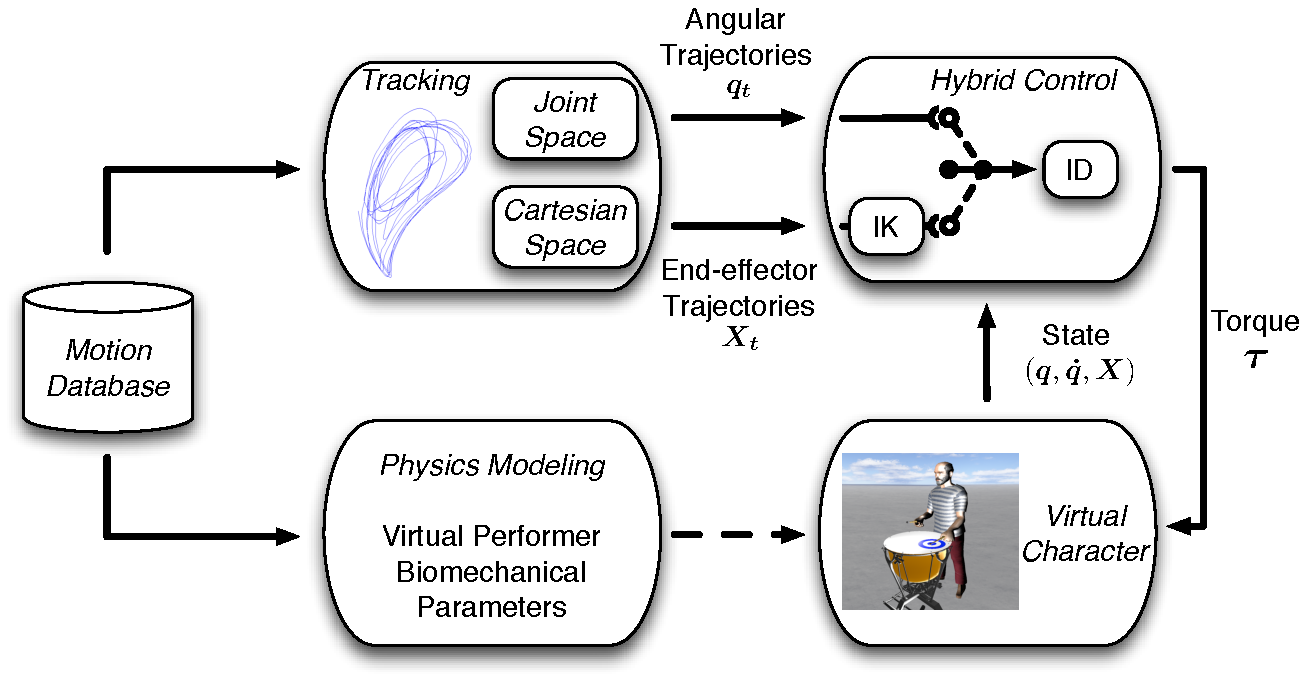
\includegraphics[width=0.9\linewidth]{Chapters/5/Pics/Pdf/hybridControl.pdf}
%	\vspace{-0.5cm}
	\caption[Hybrid physics-based motion control and synthesis]{Hybrid physics-based motion control and synthesis. The \emph{Motion Capture Database} is used for the physics modeling of the \emph{Virtual Character}, and for expressing two levels of \emph{Tracking}. These two levels allow the physics-based motion capture tracking, either in the \emph{Joint Space} from angular trajectories $\boldsymbol{q_t}$, or in the \emph{Cartesian Space} from end-effector trajectories $\boldsymbol{X_t}$. The hybrid control involves the combination of inverse kinematics (\emph{IK}) and inverse dynamics controllers (\emph{ID}).}
	\label{fig:motionSynthesis}
\end{figure}

A more intuitive physics control of the virtual character is proposed by combining \emph{IK} and \emph{ID} controllers. Instead of directly tracking angular trajectories from the motion capture database, this tracking mode consists in extracting end-effector positions in the 3D Cartesian space. From these Cartesian targets, an \emph{IK} method computes \myequname \eqref{eq:equation2} the kinematic postures (joint vector $\boldsymbol{q_t} $= \{$q_1$, ..., $q_n$\}), which are used as the desired input of the \emph{ID} controllers (\myalgname \ref{alg:hybridControl}), thus providing the required torques to control the physical character (\myfigname \ref{fig:motionSynthesis}).

\begin{equation}
	\begin{array}{l}
		\boldsymbol{\Delta q_t} = \mathcal{J}^{-1}(\boldsymbol{q}).(\boldsymbol{X_t} - \boldsymbol{X}), \hspace{2mm} \boldsymbol{q_t} = \boldsymbol{q} + \boldsymbol{\Delta q_t} \\
		\boldsymbol{\tau} = k_s . (\boldsymbol{q_t} - \boldsymbol{q}) -  k_d . \dot{\boldsymbol{q}}
	\end{array}
\label{eq:equation2}
\eqcaption{\emph{IK} control involved in the hybrid motion control}
\end{equation}

\begin{algorithm}[H]
	%\dontprintsemicolon
	\emph{}\;

	\begin{center}
		\begin{tabular}[3cm]{rcc}
			\multirow{2}{*}{In} & $\boldsymbol{AC} = \lbrace \boldsymbol{T^K}, \boldsymbol{T^D}\rbrace$ & Articulated chain \\
				& $F_T$ & Task frequency\\
				& $F_S$ & Simulation frequency\\
				& $\boldsymbol{q}, \boldsymbol{\dot{q}}$ & Current kinematic posture of $T^K$ \\
				& $\boldsymbol{X}$ & Current end-effector position of $T^K$ \\
				& $\boldsymbol{X_t}$ & Targetted end-effector position of $T^K$ \\
			\\
			\multirow{3}{*}{Out} & $\boldsymbol{\mathcal{J}}$ & Jacobian matrix \\
				& $\boldsymbol{q_t}$ & Targetted kinematic posture of $T^K$ \\
				& $\boldsymbol{\tau}$ & Resulting torques to be exerted on $T^D$ \\
		\end{tabular}\;
	\end{center}

	\While{Read task at $F_T$}{
		\emph{}\;
		$\boldsymbol{X_t}$ $\leftarrow$ New mallet extremity\;
		\emph{}\;

		$numIKID$ = 0\;
		\emph{}\;

		\For{numIKID < $F_S$/$F_T$}{
			\emph{}\;
			\emph{** Inverse Kinematics **}\;
			$\boldsymbol{\mathcal{J}}$ $\leftarrow$ ComputeJacobian($\boldsymbol{T^K}$, $\boldsymbol{q}$)\;
			$\boldsymbol{q_t}$ $\leftarrow$ InverseKinematics($\boldsymbol{\mathcal{J}}$, $\boldsymbol{X}$, $\boldsymbol{X_t}$, $\boldsymbol{q}$)\;
			\emph{}\;
	
			\emph{** Inverse Dynamics **}\;
			$\boldsymbol{\tau}$ $\leftarrow$ InverseDynamics($\boldsymbol{q}$, $\boldsymbol{\dot{q}}$, $\boldsymbol{q_t}$)\;
			\emph{}\;
	
			\emph{** Update **}\;
			ApplyTorques($\boldsymbol{T^D}$, $\boldsymbol{\tau}$)\;
			Update($\boldsymbol{T^K}$, $\boldsymbol{T^D}$)\;
		\emph{}\;
		}
	}
	\emph{}\;

	\caption{Hybrid motion control combining \emph{IK} and \emph{ID} controllers}
	\label{alg:hybridControl}
\end{algorithm}

$\mathcal{J}$ represents the Jacobian of the system to be controlled, $\boldsymbol{X}$ and $\boldsymbol{X_t}$ represent respectively the current and target end-effector positions in the Cartesian space. The modularity of the presented approach for combining \emph{IK} and \emph{ID} controllers allows to consider any method, so that our system supports at the momemt several \emph{IK} formulations (transpose, pseudo-inverse and damped-least-squares, see section \ref{subsubsubsec:CA_MC_Kinematics_Inv}) that can be combined with simple \emph{ID} formulations. One may equally use other \emph{IK} techniques, such as learning techniques described in \citeCGA{gibet:CASA03, gibet:ISDA07}.

\myalgname \ref{alg:hybridControl} shows the principle of the hybrid motion control, composed of two nested loops. The first one concerns the task specification (mallet extremity position). Between two task updates, the second loop involves the cooperation of the \emph{IK} and \emph{ID} formulations. For example, for a task frequency of 250 Hz and a simulation frequency of 10000 Hz, the second simulation loop is called 10000/250=40 times, which can be sufficient  so that the \emph{IK} algorithm converges, and consequently ending with the \emph{ID} convergence.\\

Using such an \emph{IK} formulation necessitates the computation of the Jacobian matrix, and therefore we defined an equivalent representation of the articulated chain, both in the kinematics and dynamics spaces. The main difficulty with the coupling of both kinematics and dynamics controllers is that the convergence of the \emph{IK} algorithm is added to the difficulty of tuning the parameters of the \emph{PD} dynamic controllers. But this approach enables the manipulation of motion capture data in the 3D Cartesian space (configuration $\boldsymbol{X_t}$) instead of the angular space ($\boldsymbol{q_t}$), which is more consistent and intuitive for controlling percussion gestures, by using end-effector trajectories, for instance mallets extremities.\\


		\subsection{Results}
		\label{subsec:Synthesis_Physics_Results}

%		\subsubsection{Methodology}
%		\label{subsubsec:Synthesis_Physics_Results_Methodo}

%The physical model of the virtual character is composed of 19 joints, totalling 57 degrees of freedom. The Open Dynamic Engine \citeCGA{ode} is used for the overall motion simulation. Masses, inertia, limb lengths, as well as joint limits are estimated from real percussion performers. Concerning the hybrid control mode, different inverse kinematics methods may be combined to \emph{ID} controllers. These results use an implenentation of the Damped Least Squares method \citeCGA{wampler:SMC86}, a simple yet more robust adaptation of the pseudo-inverse regarding the singularity of the inverse kinematics problem.

%It should be noted that in all results described in the following points, we kept the same parameterization of the damped springs of the virtual character.\\

%A qualitative evaluation of the presented hybrid motion control is first conducted. The results obtained by the two tracking modes used to physically control the virtual percussionist are compared: a) motion capture tracking in joint space, involving only \emph{ID} controllers, and b) motion capture hybrid tracking in cartesian space, involving a combination of \emph{IK} and \emph{ID} controllers.\\

%Then a more quantitative evaluation is presented for quantifying the errors made by the two motion tracking modes during the simulation of various types of percussion gestures. An evaluation directed by a classification/recognition methodology analogous to chapter \ref{chapter:Analysis} is also conducted.

The physical model of the virtual character is composed of 17 joints, totalling 51 degrees of freedom. The Open Dynamic Engine \citeCGA{ode} is used for the forward dynamics simulation of the motion equations. Masses, inertia, limb lengths, as well as joint limits are estimated from real percussion performers. Concerning the hybrid control mode, many inverse kinematics methods may be involved in our cascaded control mode. These results have been obtained using an implementation of the damped-least-squares method \cite{wampler:SMC86}, a simple yet more robust adaptation of the pseudo-inverse regarding the singularity of the inverse kinematics problem. The hybrid control scheme presented previously is tested on the control of the two arms of the virtual character, tracking a sequence of percussion gestures for synthesizing whole arm movements only from the specification of the mallet extremity trajectories.

The results presented in this section compare the traditional \emph{ID} control mode to our hybrid control scheme. It should be noted that for making such a comparison possible, the parameters that can change drastically the resulting simulations have been kept constant. Such parameters include for instance the simulation rate, the recorded motion to be simulated as well as the parameterization of the damped springs composing the dynamic layer of the virtual character.\\

A qualitative evaluation of the presented hybrid motion control is first conducted. The results obtained by the two tracking modes used to physically control the virtual percussionist are compared: a) motion capture tracking in joint space, involving only \emph{ID} controllers, and b) motion capture hybrid tracking in Cartesian space, involving the cascaded combination of \emph{IK} and \emph{ID} controllers. In a second time, we quantitatively evaluate the two tracking modes by quantifying the errors made during the simulation of various types of percussion gestures in each control case. An evaluation directed by a classification/recognition methodology analogous to chapter \ref{chapter:Analysis} is also conducted.\\

%Then a more quantitative evaluation is presented for quantifying the errors made by the two motion tracking modes during the simulation of various types of percussion gestures. An evaluation directed by a classification/recognition methodology analogous to chapter \ref{chapter:Analysis} is also conducted.\\

Concerning the quantitative evaluation, a critical issue to consider is the metric used for evaluating the effectiveness of our hybrid solution compared to traditional \emph{ID} control. A few works have addressed the question of the user sensibility to various motion metrics \citeCGA{reitsma:TOG03, ren:TOG05}. In this work, the ballistic nature of percussion motion makes it however easy to conduct an extensive evaluation by focusing on mallet extremity trajectories. We also show that our solution leads to a coherent motion in the joint space for specific degrees of freedom that are shown to be of paramount importance in percussion playing.


			\subsubsection{Qualitative Evaluation}
			\label{subsubsec:Synthesis_Physics_Results_QualitativeEval}

%For this qualitative evaluation, we ran the simulation of a set of pre-recorded percussion gestures (\emph{French} grip, \emph{legato}). \myfigname \ref{fig:mocapIKIDEvaluation} compares raw data from captured motion with the two modes of control (\emph{ID} only, and the hybrid combination of \emph{IK} and \emph{ID}).\\

%The hybrid control scheme tracks one percussion gesture for synthesizing whole arm movements only from the specification of the tip of the mallets trajectories. \myfigname \ref{fig:mocapIKIDEvaluation} (top) presents the comparison between raw motion capture data and data generated by the \emph{IK} process. It shows that data generated by the \emph{IK} formulation are consistent with real ones, especially for the elbow flexion angle that is one of the most important degree of freedom of the arm in percussion gestures (especially during preparatory phases \citeIPA{bouenard:ENACTIVE08}).\\
 
%We finally present the comparison of the two control modes (\emph{ID} control only and hybrid control) in \myfigname \ref{fig:mocapIKIDEvaluation} (bottom). One interesting issue is the accuracy of the hybrid control mode compared to the simple \emph{ID} control. This observation lies in the fact that the convergence of motion capture tracking is processed in the joint space in the case of \emph{ID} control, adding and amplifying multiple errors on the different joints and leading to a greater error than processing the convergence in the Cartesian space for the hybrid control.\\

%Although such cascaded chain of \emph{IK} and \emph{ID} controllers run in real-time, the main drawback of this improvement is however the additional computationnal cost of the \emph{IK} algorithm which is processed at every simulation step. It provides nevertheless a more flexible motion edition technique for controlling a fully physics-based virtual character, that eases the co-articulation between successive motion units. %This is illustrated in \myfigname \ref{fig:impro}, which shows the creation of a gesture score from a musical score, and the animation of the virtual percusionist following this score.

For this qualitative evaluation, we ran the simulation of a set of pre-recorded percussion gestures (\emph{French} grip, \emph{legato}). Figure \ref{fig:mocapIKIDEvaluation} compares raw data from captured motion with the two modes of control (\emph{ID} only, and the hybrid combination of \emph{IK} and \emph{ID}).\\

\begin{figure}%[H]
	\begin{center}
		\subfigure[]{\label{fig:mocapIKIDEvaluation1}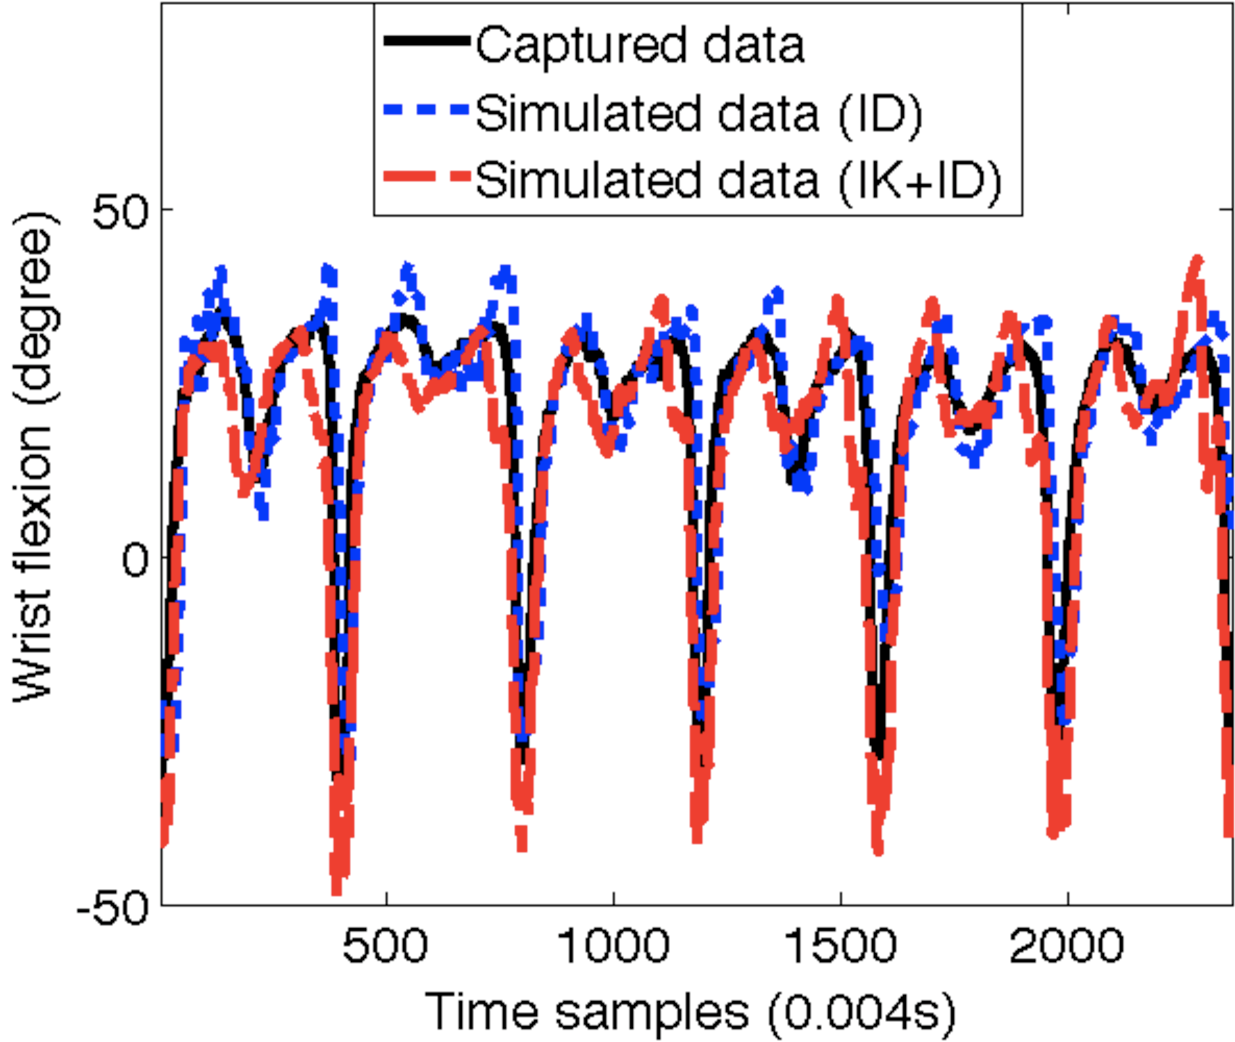
\includegraphics[width=0.45\linewidth]{Chapters/5/Pics/Pdf/wrist_angle2.pdf}}
		\hspace{6mm}
		\subfigure[]{\label{fig:mocapIKIDEvaluation4}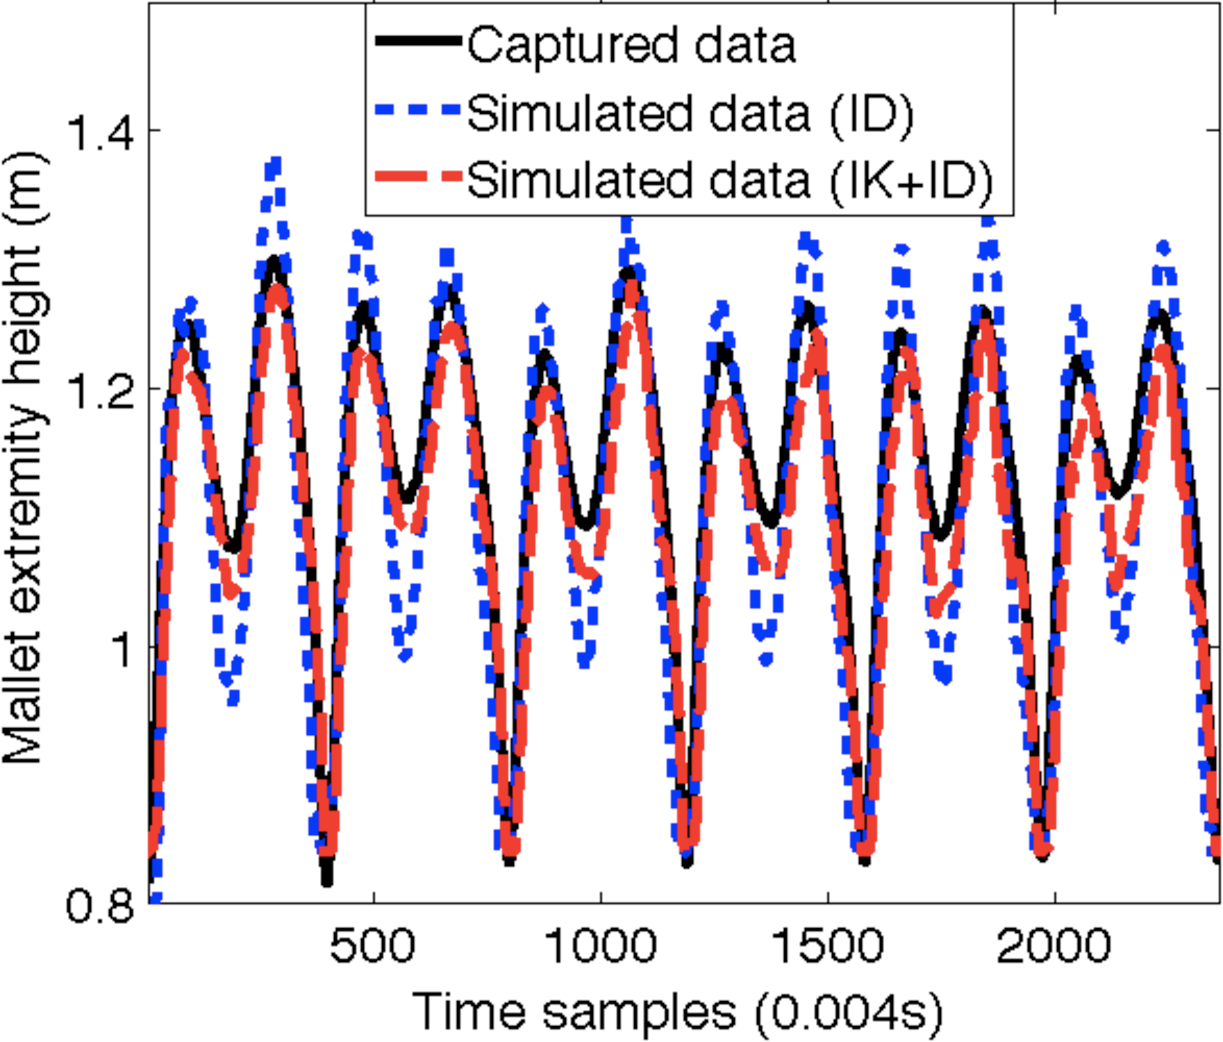
\includegraphics[width=0.45\linewidth]{Chapters/5/Pics/Pdf/drumstick_pos.pdf}}\\
		\subfigure[]{\label{fig:mocapIKIDEvaluation2}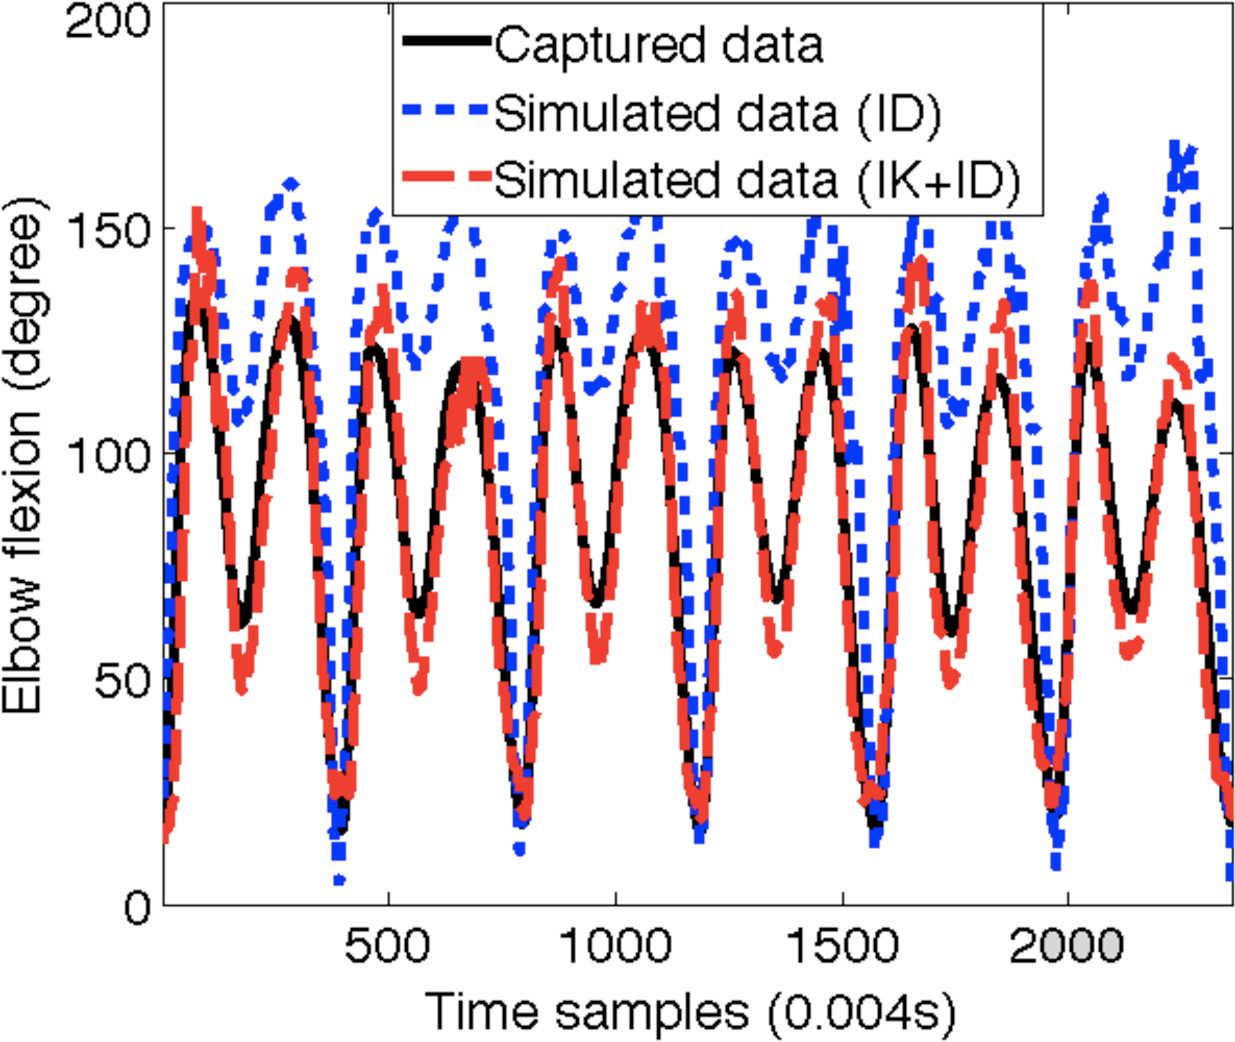
\includegraphics[width=0.45\linewidth]{Chapters/5/Pics/Pdf/elbow_angle.pdf}}
		\hspace{6mm}
		\subfigure[]{\label{fig:mocapIKIDEvaluation5}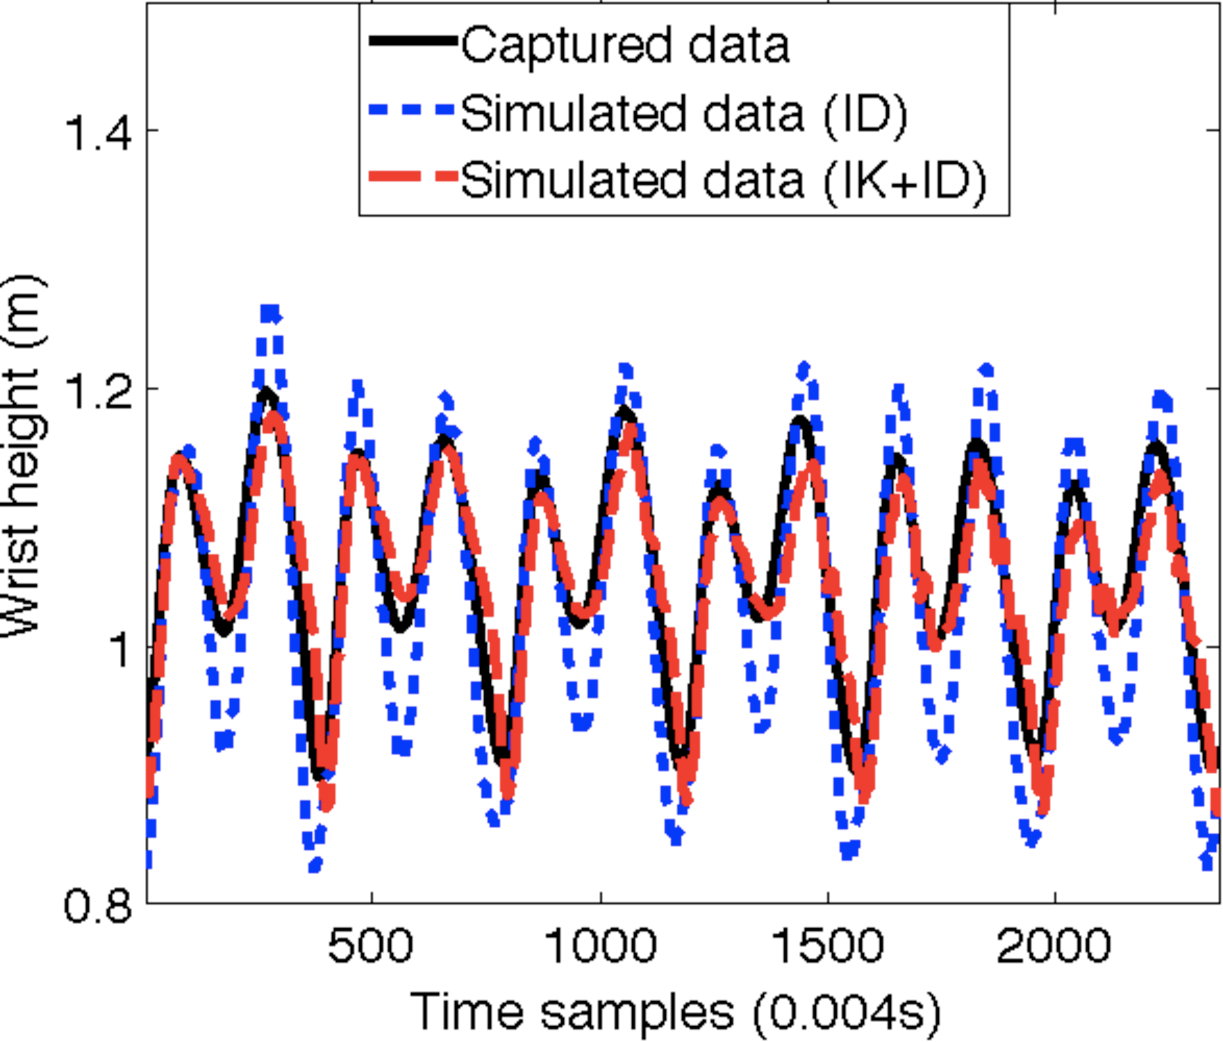
\includegraphics[width=0.45\linewidth]{Chapters/5/Pics/Pdf/wrist_pos.pdf}}\\
		\subfigure[]{\label{fig:mocapIKIDEvaluation3}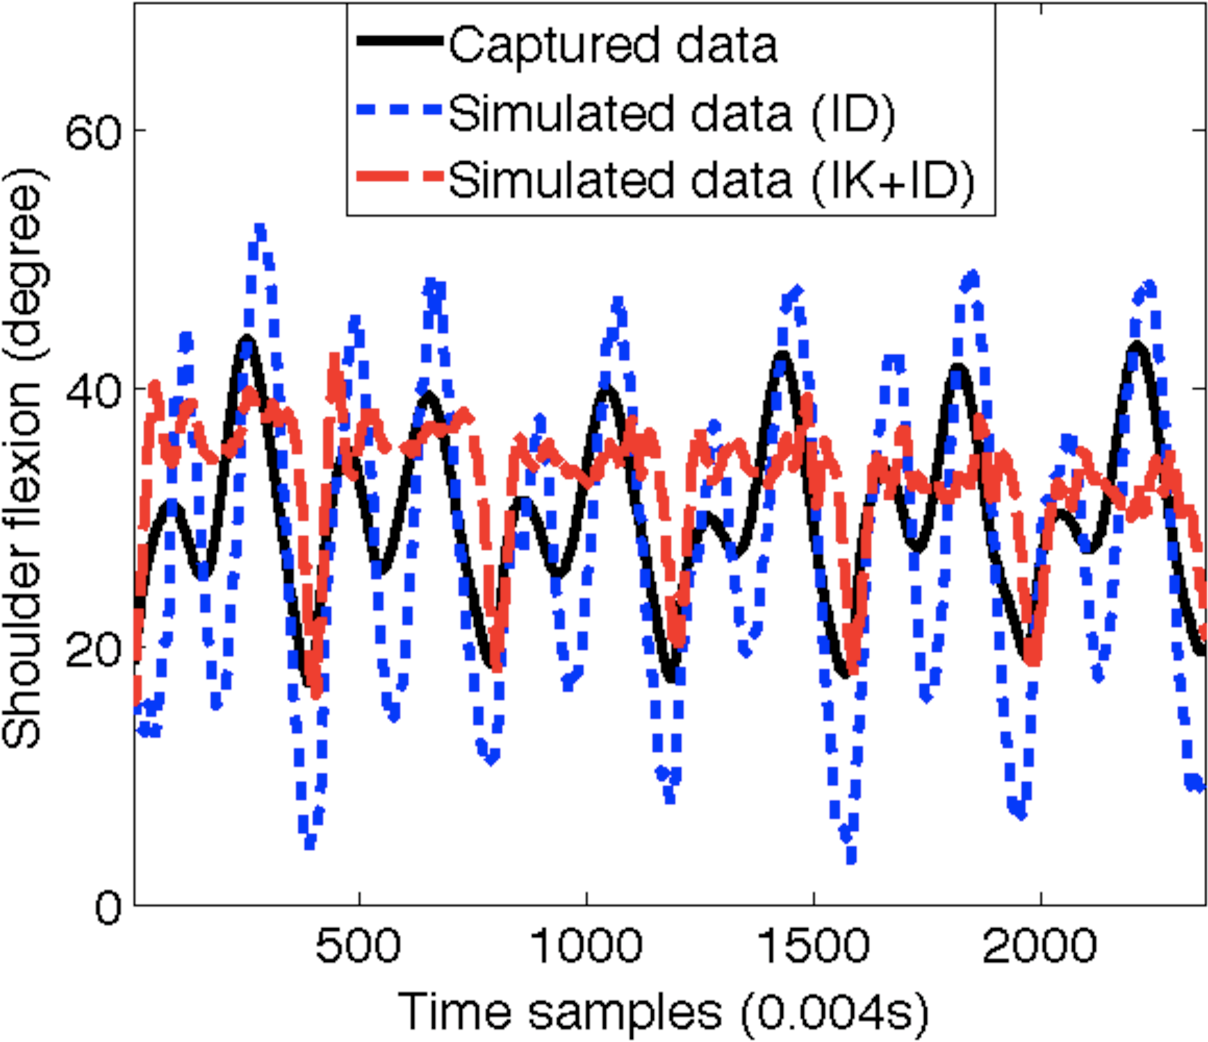
\includegraphics[width=0.45\linewidth]{Chapters/5/Pics/Pdf/shoulder_angle.pdf}}
		\hspace{6mm}
		\subfigure[]{\label{fig:mocapIKIDEvaluation6}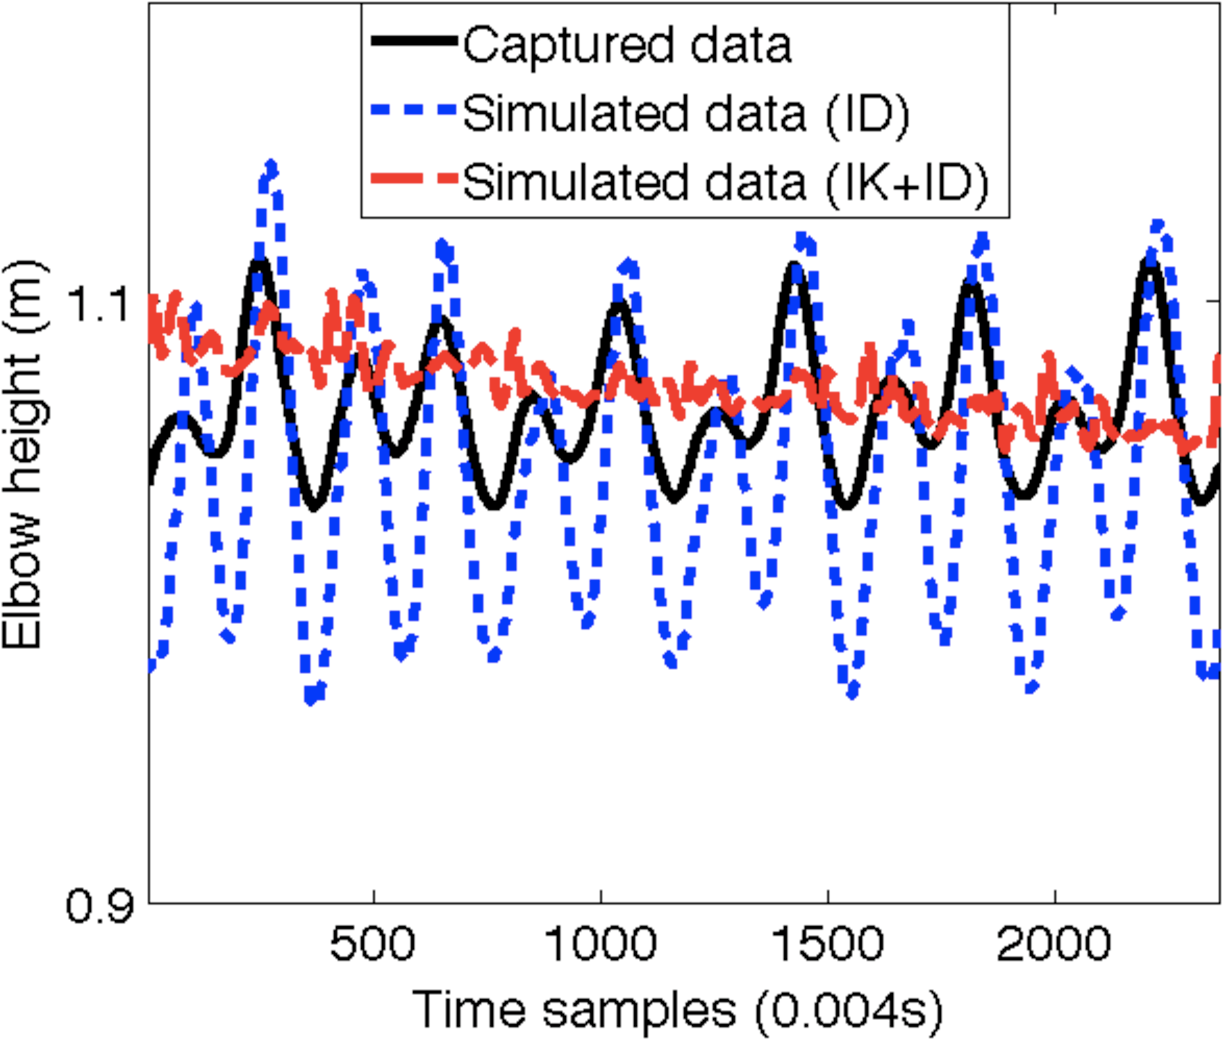
\includegraphics[width=0.45\linewidth]{Chapters/5/Pics/Pdf/elbow_pos.pdf}}
	\end{center}
	\vspace{-0.6cm}
	\caption[Comparison of captured and simulated trajectories]{Comparison of captured and simulated trajectories using the two motion control schemes: (a), (c) and (e) resp. for wrist, elbow and shoulder flexion angles, (b), (d) and (f) resp. for mallet, wrist and elbow height positions.}
	\label{fig:mocapIKIDEvaluation}
\end{figure}

\myfigname \ref{fig:mocapIKIDEvaluation1}, \ref{fig:mocapIKIDEvaluation2} and \ref{fig:mocapIKIDEvaluation3} present the comparison between raw motion capture data and data generated by the two control modes for wrist, elbow and shoulder flexion angle trajectories. These results show that data generated by the \emph{IK} involved in the hybrid control mode are consistent with real ones, especially for wrist and elbow trajectories. Data generated by our hybrid solution is more accurate compared to \emph{ID} control, this latter shows indeed a motion exaggeration that tends to be avoided by our solution.

More specifically about shoulder flexion angle, \myfigname \ref{fig:mocapIKIDEvaluation3}, it seems that the \emph{IK} process looses the pattern of the original motion, while leading to more accurate extrema occuring at beat impacts compared to \emph{ID} control. This loss is however of lower importance in percussion gestures, as attested in \cite{bouenard:ENACTIVE08} where it is argued that wrist and elbow angle trajectories are one of the most important degrees of freedom in percussion arm mechanisms.\\
 
We also present the result comparison of the two control modes concerning height trajectories for the mallet extremity, wrist and elbow in \myfigname \ref{fig:mocapIKIDEvaluation4}, \ref{fig:mocapIKIDEvaluation5} and \ref{fig:mocapIKIDEvaluation6}. One interesting issue is the accuracy of the hybrid control mode compared to the simple \emph{ID} control. The motion exaggeration observed previously in joint flexion trajectories in the case of \emph{ID} control is propagated on joint position trajectories. Conversely, our hybrid solution leeds to a more accurate tracking in joint position trajectories. This observation lies in the fact that the convergence of motion capture tracking is processed in the joint space in the case of \emph{ID} control, adding and amplifying multiple errors on the different joints and leading to a greater error than processing the convergence in the Cartesian space for the hybrid control.

One limitation however arises in elbow position trajectories. While the \emph{ID} control mode results again in an amplified motion, our hybrid control solution results in a loss in the motion pattern of original data. The elbow position trajectory resulting from the hybrid control mode leads to a more stiff and somewhat constant motion. This can be related to the inverse kinematics scheme which does not include any secondary goals, as already pointed out in \citeCGA{klein:TSMC83}. This may be explained also by the fact that the \emph{IK} algorithm favorizes the accuracy of the most distal joints compared to joints at the basis of the articulated chain. Another reason to this limitation could be the influence of the physics simulation on the convergence of the inverse kinematics scheme.\\

Although such cascaded chain of \emph{IK} and \emph{ID} controllers runs in real-time, the main drawback of this improvement is however the additional computationnal cost of the \emph{IK} algorithm which is processed at every simulation step. It provides nevertheless a more flexible motion edition technique for controlling a physics-based virtual character solely by end-effector trajectories. It also provides a consistent control scheme as regards to the preliminary analysis conducted in chapter \ref{chapter:Analysis}.

%\newpage
%\vfill

%\begin{figure}[H]
%	\centering
%	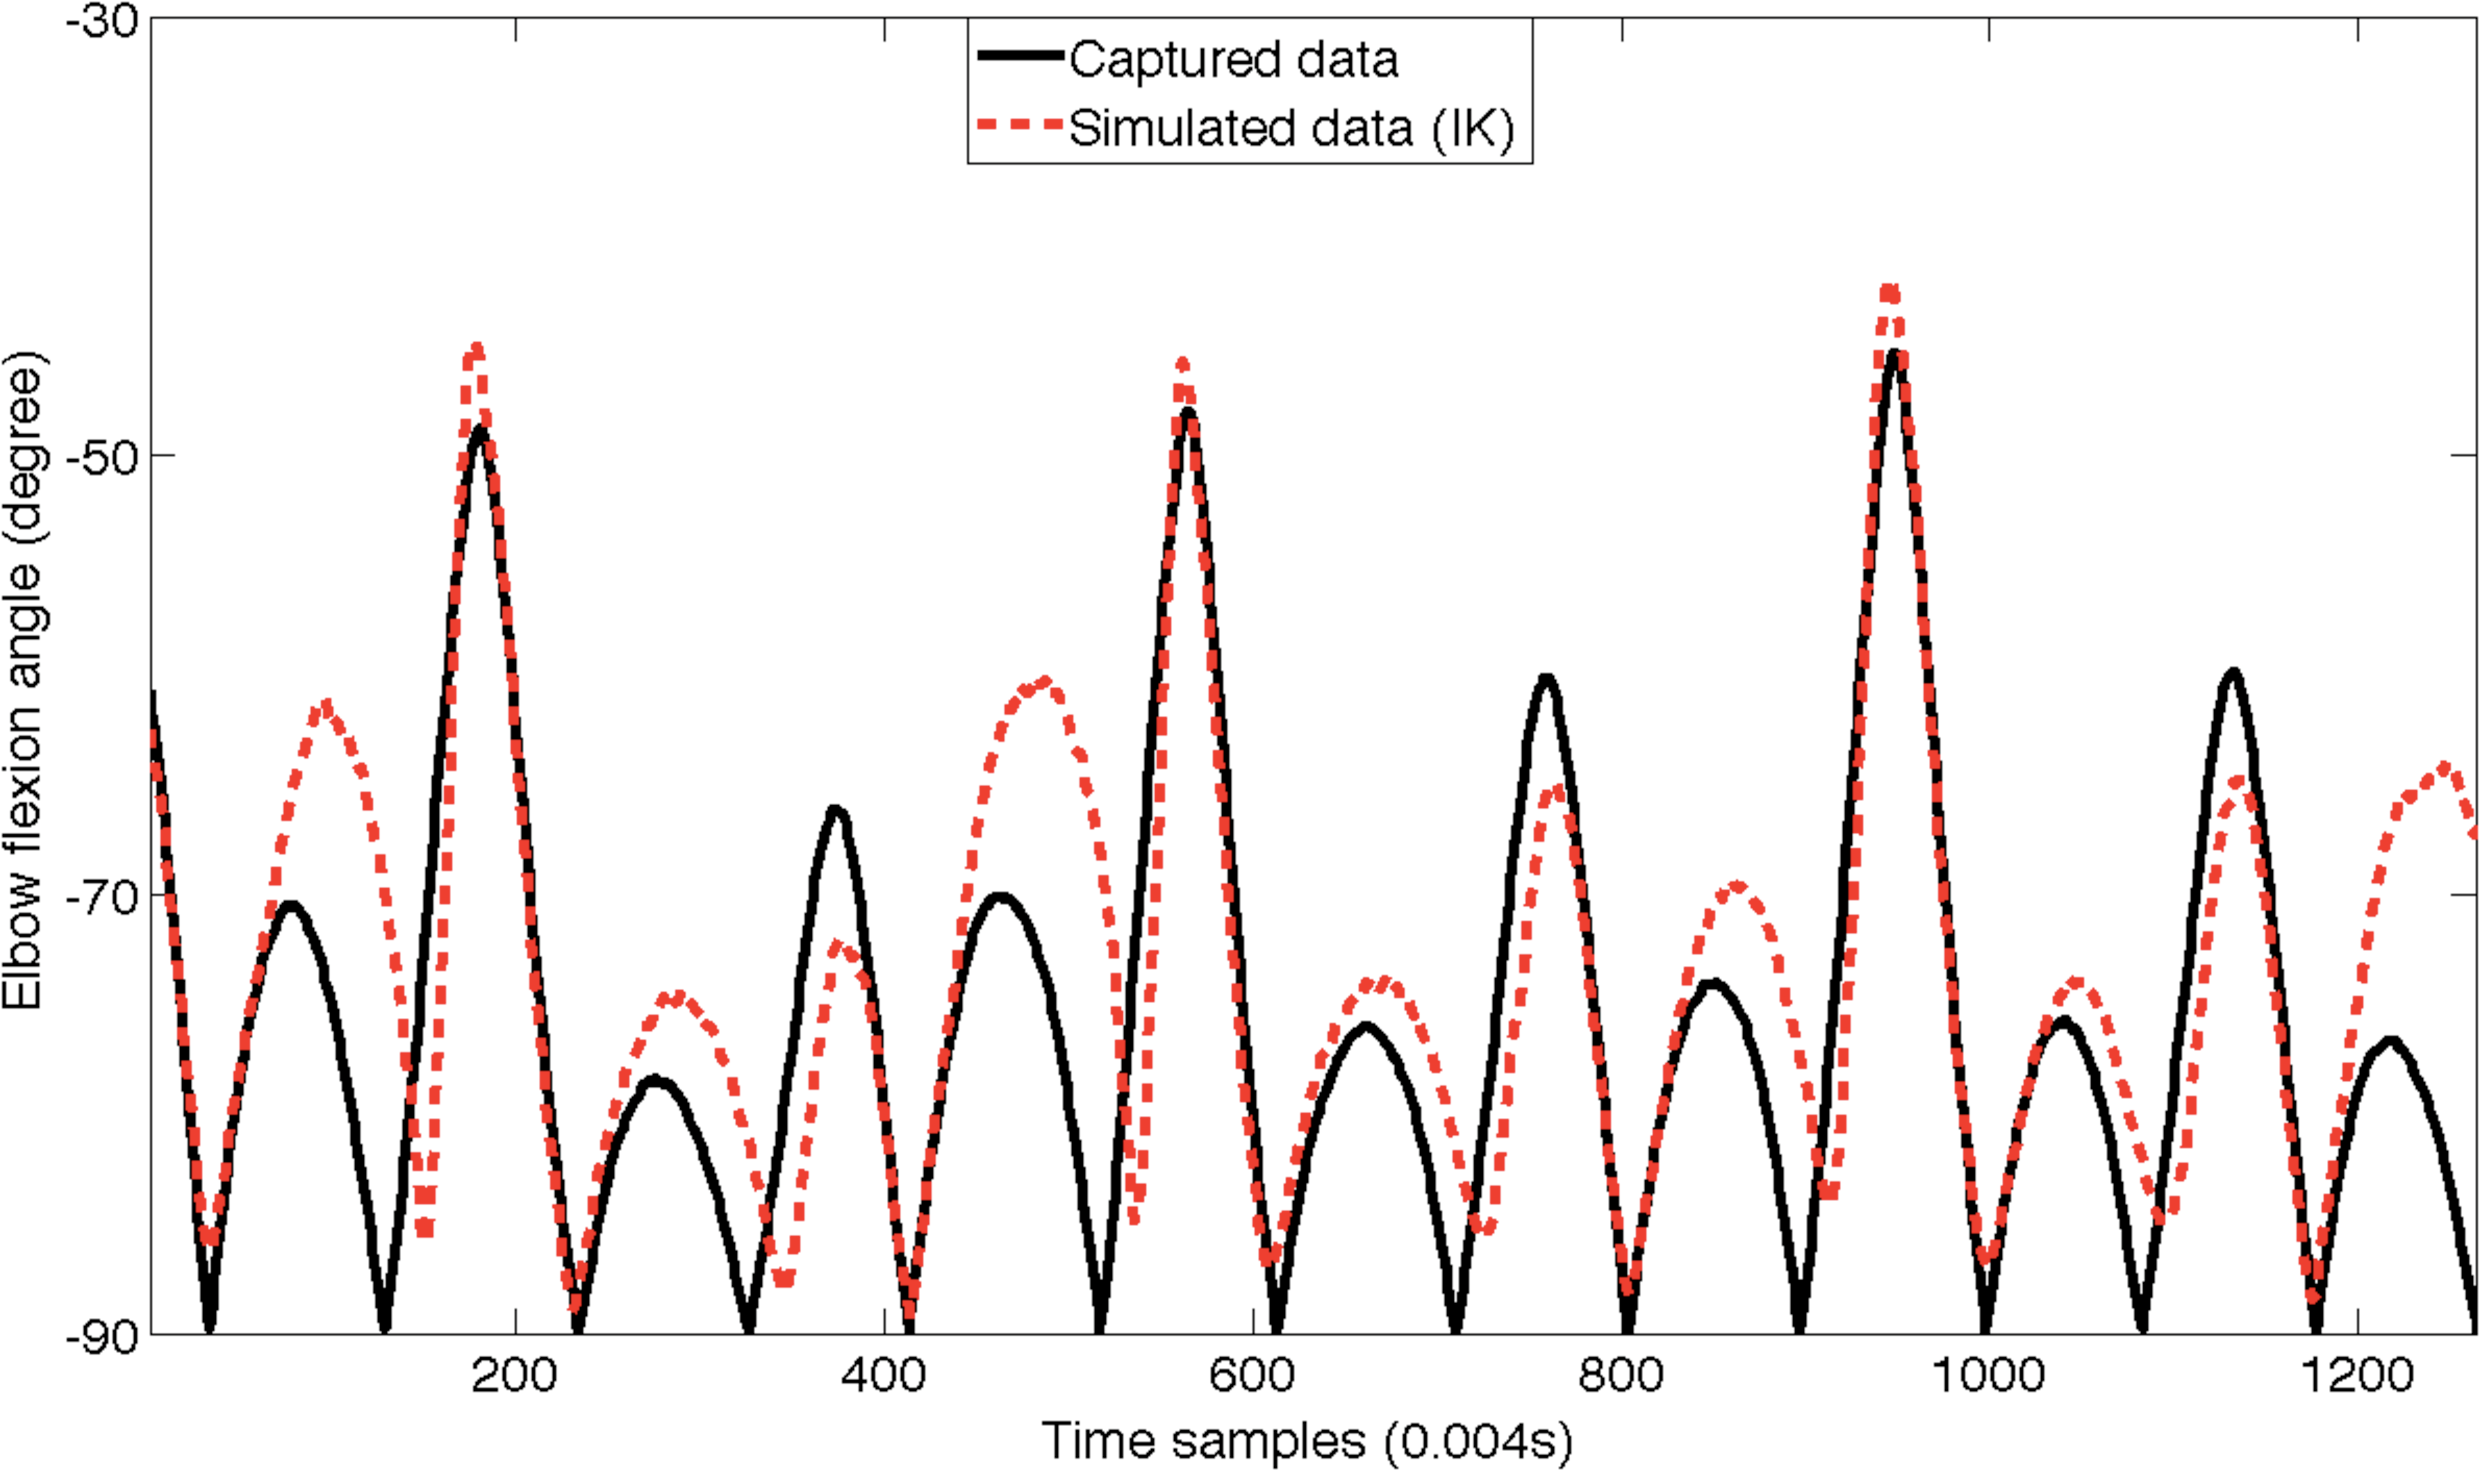
\includegraphics[width=\linewidth]{Chapters/5/Pics/Pdf/MoCap_IK_Comparison.pdf}
%	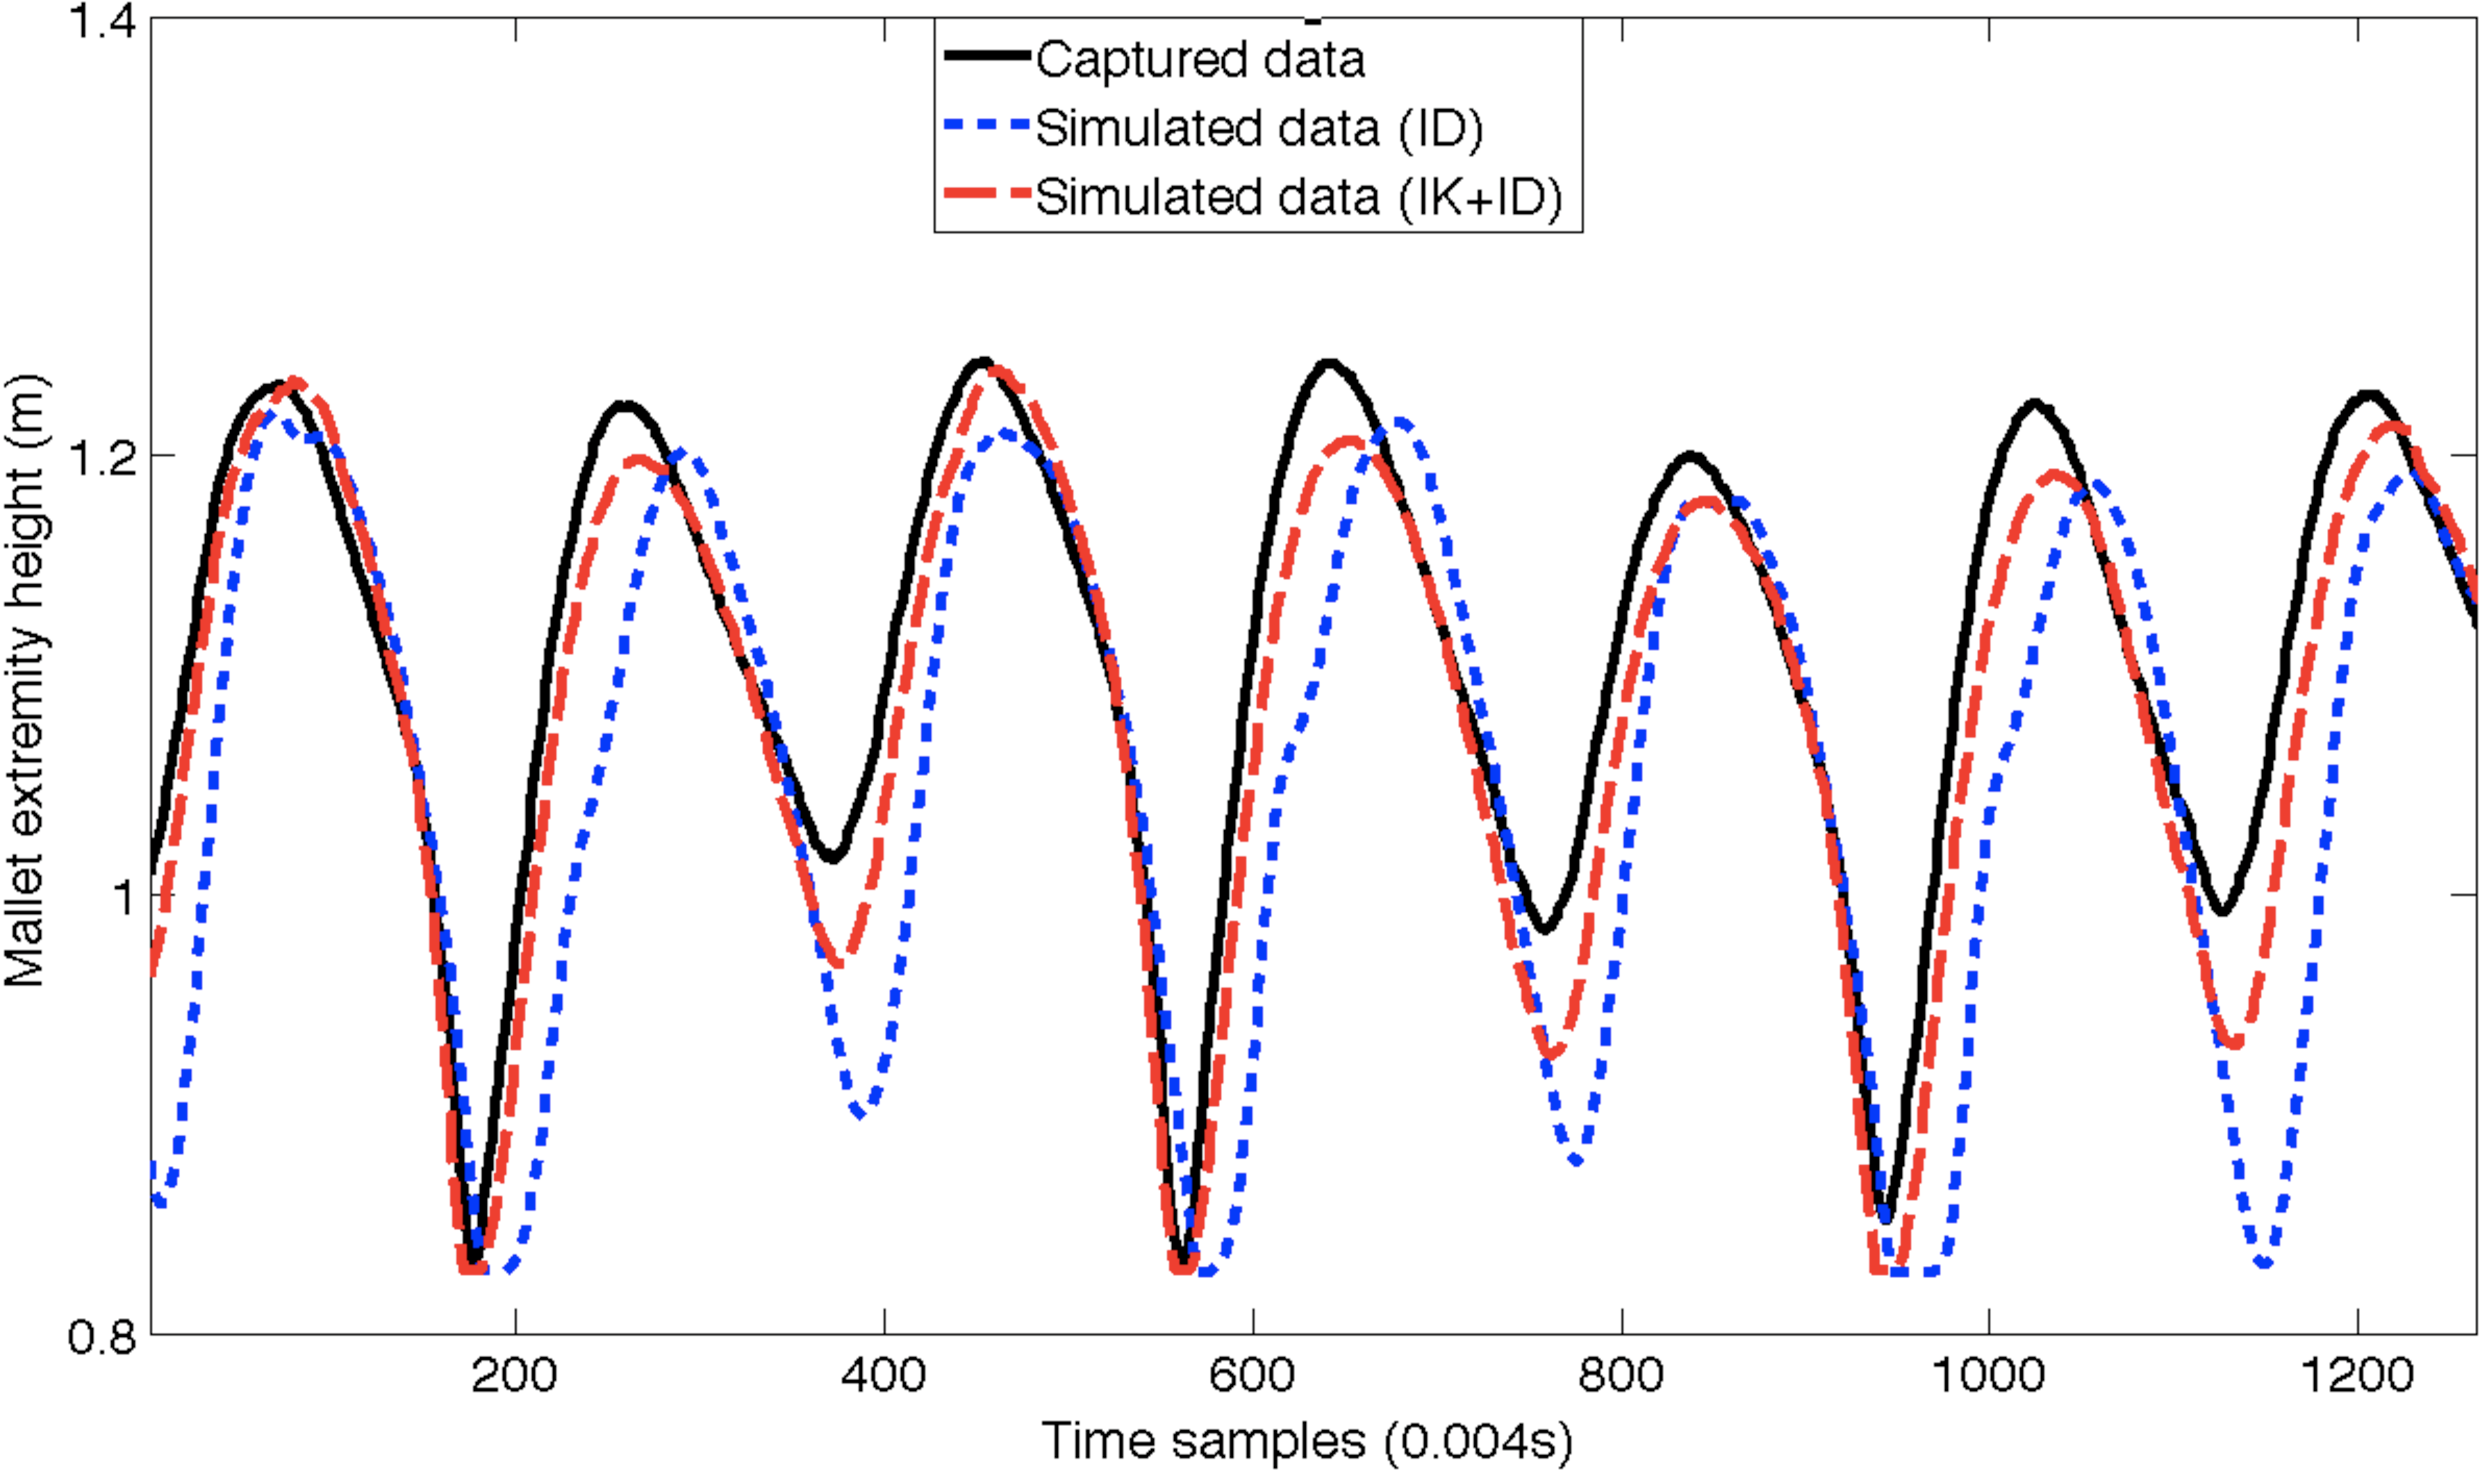
\includegraphics[width=\linewidth]{Chapters/5/Pics/Pdf/MoCap_ID_IKID_Comparison.pdf}
%	\caption[Comparison of captured and simulated mallet trajectories for a \emph{legato} stroke]{Comparison of captured and simulated mallet trajectories for a \emph{legato} stroke, using the two motion control schemes. Top: comparison of elbow flexion angle trajectories, original motion data (plain) vs. data generated by the \emph{IK} algorithm (dash). Bottom: comparison of mallet trajectories, original motion capture data (plain) vs. joint space (\emph{ID}) physics tracking (little dash) vs. cartesian space (\emph{IK} + \emph{ID}) physics tracking (large dash).}
%	\label{fig:mocapIKIDEvaluation}
%\end{figure}


			\subsubsection{Quantitative Evaluation}
			\label{subsubsec:Synthesis_Physics_Results_QuantitativeEval}

%An extensive evaluation of the two control modes is presented in \myfigname \ref{fig:rms}. This takes into account the test of the two control algorithms on 200 simulation trials for various gesture variations (from top to bottom: \emph{legato}, \emph{tenuto}, \emph{accent}, \emph{vertical accent} and \emph{staccato}). For each simulation trial, the root mean square error and standard deviation is processed compared to a gesture unit initially chosen in the motion capture database.\\

%From these results, one can easily conclude that the cascaded hybrid combination of \emph{IK} and \emph{ID} controllers leads to a more accurate minimization of the error commited on mallet extremity trajectories of about 1 centimeter, compared to simple \emph{ID} controllers. The standard deviation along simulation trials are also more minimized for the hybrid motion paradigm compared to the \emph{ID} control.

An extensive evaluation of the two control modes is presented in \myfigname \ref{fig:rms}. This takes into account the test of the two control algorithms on 200 simulation trials for various playing modes (from top to bottom: \emph{legato}, \emph{tenuto}, \emph{accent}, \emph{vertical accent} and \emph{staccato}). \myfigname \ref{fig:playingModes} shows examples of longitudinal-vertical phases of the mallet extremity position for each playing mode. This emphasizes that these playing modes present drastically different gesture dynamics in mallet motion, especially regarding its longitudinal and vertical amplitude. Each simulation trial corresponds to a gesture unit that is simulated according to the two control modes. The root mean square error and its standard deviation are processed as regards to the mallet extremity compared to the corresponding motion initially chosen in the motion capture database.\\

From the results presented in \myfigname \ref{fig:rms}, one can easily conclude that the cascaded hybrid combination of \emph{IK} and \emph{ID} controllers leads to a more accurate minimization of the error commited on mallet extremity trajectories of about 1 centimeter, compared to simple \emph{ID} controllers. The standard deviation along simulation trials are also more minimized for the hybrid motion paradigm compared to the \emph{ID} control.\\ %Such a difference of 1 centimeter in the average errors between the two control modes can be considered as negligeable. However the mallet extremity informations around the beat impacts can change drastically the nature of the resulting sounds.\\

\begin{figure}[H]
	\begin{center}
		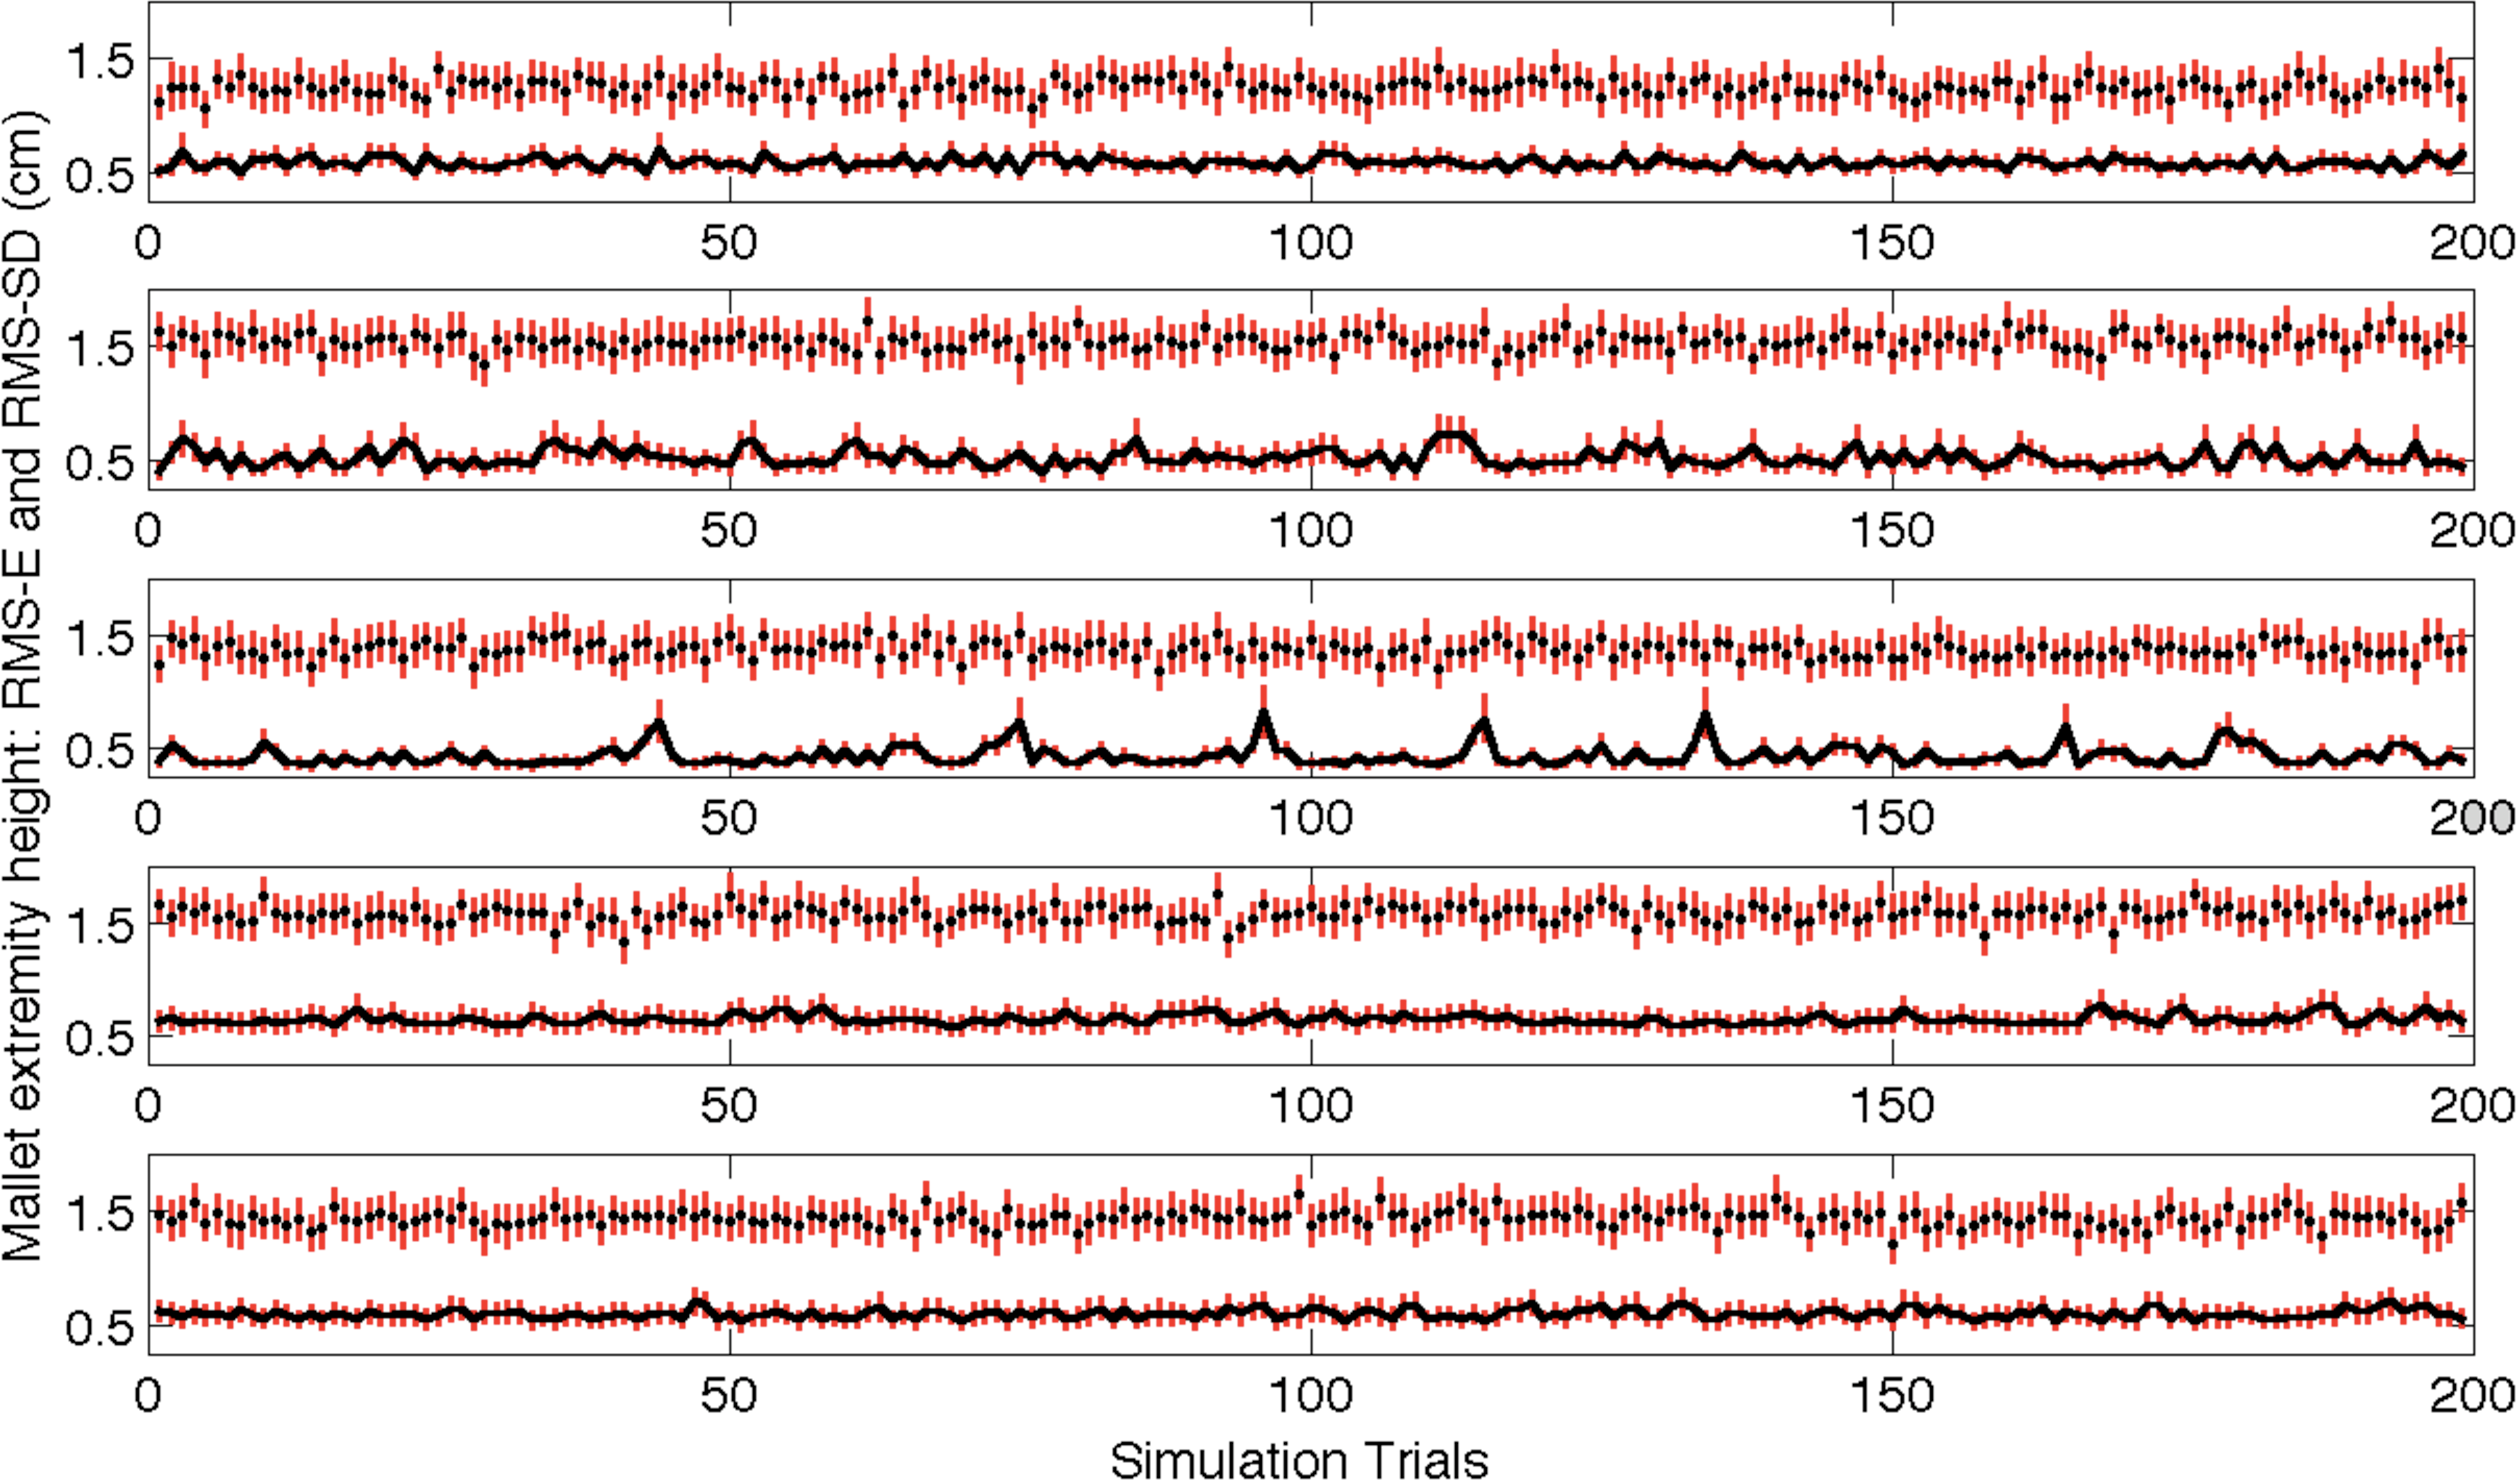
\includegraphics[width=\linewidth]{Chapters/5/Pics/Pdf/RMSE-RMSD.pdf}
	\end{center}
	\vspace{-0.5cm}
	\caption[Comparison of RMS errors between captured and simulated mallet trajectories for various playing modes]{Comparison of RMS errors between captured and simulated mallet trajectories for various playing modes, using the two motion control schemes: \emph{ID} (point line) and \emph{IK + ID} (plain). For each playing mode (from top to bottom: \emph{legato}, \emph{tenuto}, \emph{accent}, \emph{vertical accent} and \emph{staccato}), Root Mean Square Error (RMS-E, black) and Standard Deviation (RMS-SD, red) are computed on 200 simulation trials.}
	\label{fig:rms}
\end{figure}

It should be noted that this average difference of 1 centimeter of accuracy cannot be considered as negligeable, since the sound synthesis model taking mallet extremity informations around the beat impacts can change drastically the nature of the resulting sounds. For instance, in the case of modal sound synthesis models, the accuracy of mallet extremity trajectories is of paramount importance since it will change the selection of the excited mode shapes.\\

Another evaluation method has been considered for insuring the accuracy of the hybrid motion control scheme. In an analous manner to the evaluation of percussion playing characteristics in chapter \ref{chapter:Analysis}, a classification/recognition methodology has been adopted. A SVM classifier with RBF kernel functions has been trained with the extracted parameters described in section \ref{sec:Analysis_TimpaniAnalysis} from motion capture data, thus forming the training set. These gesture characteristics have also been extracted from the 200 simulations trials, which are this time forming the query set. The results of the classification/recognition of simulated playing modes (\emph{legato}, \emph{tenuto}, \emph{accent}, \emph{vertical accent} and \emph{staccato}) are summarized in the confusion matrix in \mytabname \ref{tab:recognitionFrenchVariationsSim}.
 
\begin{table}%[H]
	\centering
	\caption[SVM recognition of simulated \emph{French} grip playing modes]{SVM recognition of simulated \emph{French} grip playing modes (in percentage of success) using the combination of mallet velocity and acceleration extrema presented in Fig. \ref{fig:classifParameters}}
	\vspace{2mm}
	\begin{tabular}{||x{1.9cm}||x{1.9cm}|x{1.9cm}|x{1.9cm}|x{1.9cm}|x{1.9cm}||} \hline
		\small{$Training$ / $Test$} & \small{$Legato$} & \small{$Tenuto$} & \small{$Accent$} & \small{$V.Accent$} & \small{$Staccato$}		\tabularnewline \hline \hline
		\small{$Legato$} & 		\small{\textbf{92.6}} & \small{4.8} & \small{0} & \small{2.6} & \small{0} 	\tabularnewline \hline
		\small{$Tenuto$} & 		\small{3.7} & \small{\textbf{94.2}} & \small{1.2} & \small{0.9} & \small{0}	\tabularnewline \hline
		\small{$Accent$} & 		\small{2.5} & \small{0} & \small{\textbf{96.4}} & \small{0} & \small{1.1}	\tabularnewline \hline
		\small{$V.Accent$} & 	\small{0.5} & \small{0.6} &	\small{0} & \small{\textbf{93.9}} & \small{4.7}	\tabularnewline \hline
		\small{$Staccato$} & 	\small{0} & \small{0} & \small{0.5} & \small{4.4} & \small{\textbf{95.1}}	\tabularnewline \hline
	\end{tabular}
	\label{tab:recognitionFrenchVariationsSim}
\end{table}

These results attest the consistency of the novel hybrid motion control scheme presented in this section, giving an average recognition rate of more than 94{\%} of success for the simulated playing modes.


		\subsection{Conclusion}
		\label{subsec:Synthesis_Physics_Conclusion}

We presented in this section the derivation of the modeling and motion control of a physical model of a virtual performer which has the particularity of merging two complementary (kinematics and dynamics) representations. We also derived consequently a novel hybrid motion control scheme dedicated to percussion gestures that allows the control of the physical virtual performer solely by the specification of mallet extremity trajectories. We have particularly shown that this hybrid motion control can be more effective than simple \emph{ID} controllers for percussion gestures. Moreover, in an edition step, managing the control of a physical model only by 3D Cartesian targets is more convenient than handling whole kinematic postures.\\

From a musical point of view, and according to the conclusions of the analysis study conducted in chapter \ref{chapter:Analysis}, such an hybrid motion control scheme is also more consistent than \emph{ID} control as regards to percussion tasks, since our hybrid control scheme only needs the specification of mallet extremity trajectories. In the next section, we focuse on the interaction between motion and sound simulations (\myfigname \ref{fig:overview}) so that the simulated percussion actions of the virtual performer can influence the sound production process.

%%%%%%%%%%%%%%%%%%%%%%%%%%%%%%%%%%%%%%%%%%%%%%%%%%%%%%%%%%%%%%%%%%%%%%%%%%%%%%%%%%%%%%%%%%%%%%%%%%%%%%%%%%%%%%%%%%%%


%%%%%%%%%%%%%%%%%%%%%%%%%%%%%%%%%%%%%%%%%%%%%%%%%%%%%%%%%%%%%%%%%%%%%%%%%%%%%%%%%%%%%%%%%%%%%%%%%%%%%%%%%%%%%%%%%%%%

	\section{Interaction between Motion and Sound Synthesis}
	\label{sec:Synthesis_Control}

We propose a general architecture (\myfigname \ref{fig:interaction}) that allows to simultaneously and asynchronously run the physics simulation of percussion gestures, graphics and sound rendering processes, as well as to handle their interaction in real-time. This architecture is effective for managing different modalities and data types, and for specifying at the physics level the interaction between these former.

	\subsection{Asynchronous Client-Server Architecture}
	\label{subsec:Synthesis_Control_InteractionArchitecture}

\begin{figure}
	\centering
	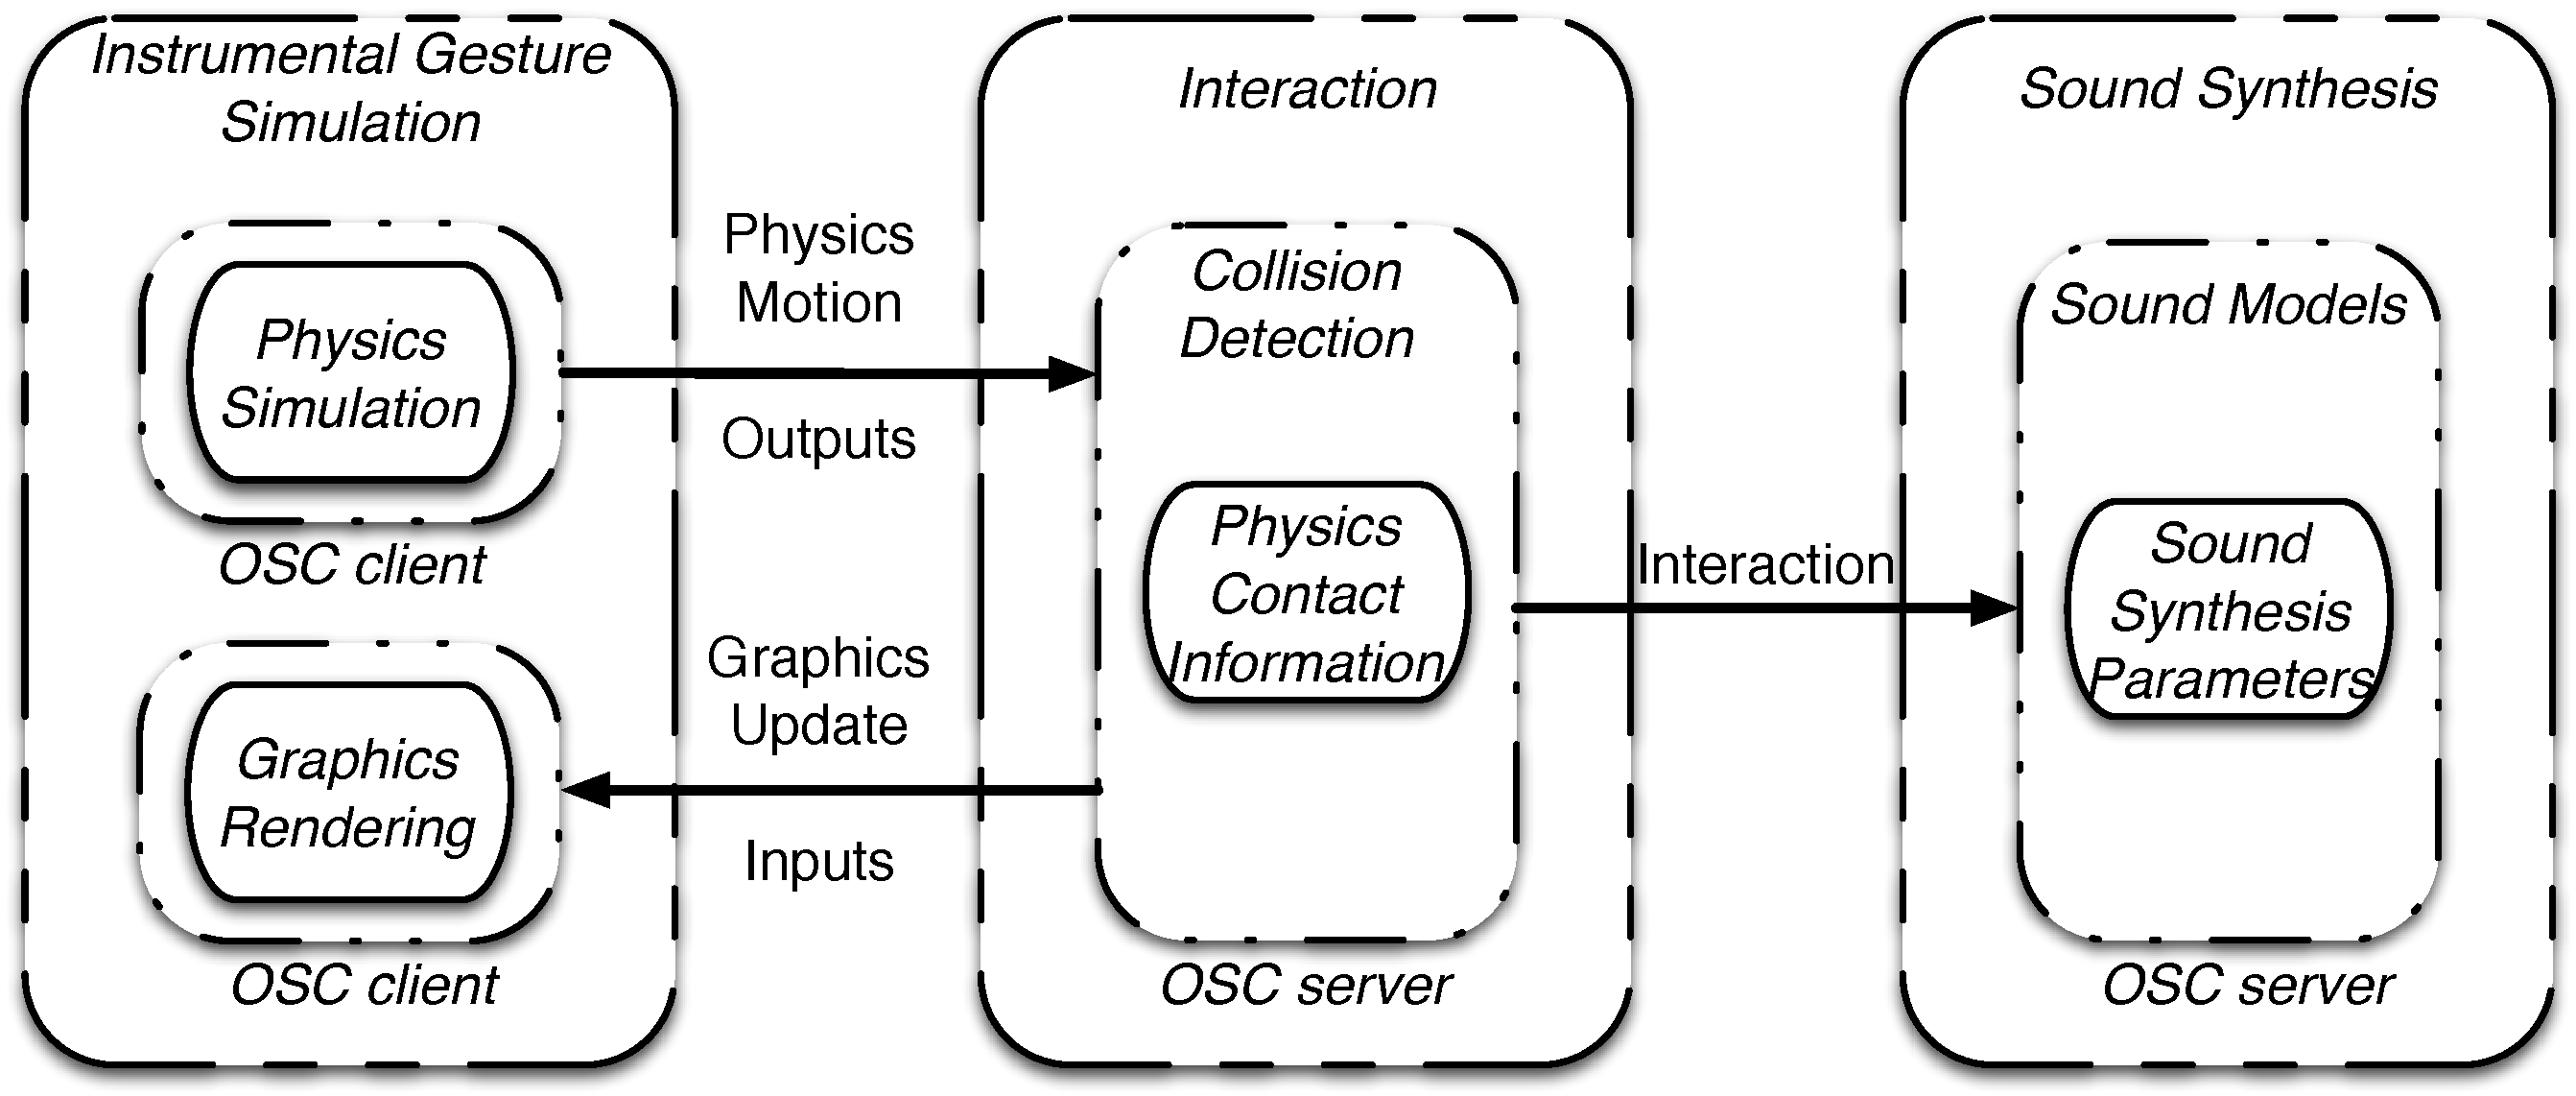
\includegraphics[width=\linewidth]{Chapters/5/Pics/Pdf/interaction2.pdf}
%	\vspace{-0.5cm}
	\caption[Asynchronous server-client architecture of our system]{Asynchronous server-client architecture of our system.}
	\label{fig:interaction}
\end{figure}

Our system makes possible the multimodal integration, interaction and synchronization of visual and sounding media, and is composed of four components represented as physics, graphics, interaction and sound managers.\\

Multimodal processes such as graphics and sound rendering are fundamently different, and achieving a real-time interaction between both of them can be hazardous. The first difficulty that appears when managing such media is their discrepency in time constants: graphics rendering is usely admitted effective at about 33Hz, whereas sound rendering needs a higher time sample ate around 44kHz. Moreover, the graphics rendering is the visible layer of a far more demanding process that is the physics simulation, requiring the handling of two other different time rates since our method relies on motion capture tracking: the original motion capture time rate and the time step of the physics simulation. An approach could consist in running synchronously every manager at the sound rate, but such an approach would fall short in real-time considerations.\\

We therefore propose an asynchronous client-server scheme for handling the interaction between the physics, graphics and sound managers. This enables the possible distribution of the different managers on distinct platforms, thus reducing the computational cost of each manager and its impact on the others.

For this purpose, we define a communication layer between the managers, based on the  Open Sound Control (\emph{OSC}) communication protocol. The \emph{OSC} protocol has been primarly designed to enable the networking and interoperability between interactive computer music applications \citeCGA{wright:OS05}. Its scheme is based on a ''transport-independant'' server-client relationship, supporting any network technology (ethernet or wireless, UDP or TCP/IP) and serial connection. Similarly to MIDI, the \emph{OSC} scheme is based on the interaction of communicative points and assigns values to these. OSC differs fondamuntally from MIDI in handling namespaces, data types and time retrieval. \emph{OSC} features intuitive naming and adressing rules (on the contrary to MIDI byte encoding), as well as an extended set of adresses and namespaces (compared to the limited and limiting six channels of MIDI). \emph{OSC} allows also the transmission of any type of structure of any size, even MIDI data, providing a standard for many software or hardware developpments. Eventually, \emph{OSC} features message time tagging for managing priority and anticipating future events. For a complete derivation of \emph{OSC} principles and functionalities, readers are refered to \citeCM{wright:NIME03, freed:NIME09, osc}.
		
The asynchronous exchange of data is materialized here by the interaction between the output of motion synthesis and the input of sound synthesis. Events produced during the physical simulation are dealt by the interaction module which feeds the sound synthesis processes and the visual outputs.


		\subsection{Motion-Sound Physics Interaction}
		\label{subsec:Synthesis_Control_InteractionMapping}

For sound synthesis, we consider in our work the modal synthesis technique. Note however that the modularity of our system allows to plug any sound synthesis model to the instrumental gesture simulation. Modal synthesis is an efficient way of representing the vibrations of resonating objects as the motion simulation of systems composed of masses connected with springs and dampers (cf. section \ref{subsubsubsec:CM_SS_Physics_SO}). This physically-based approach enables the direct modeling of the contact force impact and its effect on mode shapes. According to \citeCM{avanzini:ICMC01}, this force depends on the state (displacement and velocity) of the colliding modal objects.

We define in this section a practical interaction between the instrumental gesture simulation and a modal model of a drum membrane. Let us suppose first that such a model is available, and consider a slightly modified version of the model derived in appendix \ref{sec:ssDerivation:mM} for taking into account an interaction force on the drum membrane.
The model is governed by the motion of $N$ coupled oscillators, that can be excited by a force $\boldsymbol{f}$, \myequname \eqref{eq:equation3}.

\begin{equation}
	\boldsymbol{M} . \ddot{\boldsymbol{z}}(t) + \boldsymbol{K} . \boldsymbol{z}(t) = \boldsymbol{f}
\label{eq:equation3}
\eqcaption{Modal synthesis formulation under the influence of an external force}
\end{equation}

The factorization of the problem considers a solution of the form $\boldsymbol{z}(t) = \boldsymbol{s} . \sin(\omega.t + \phi)$ where $\boldsymbol{s}$ are again refered as the \emph{modal shapes} of the system. This leads to the equivalent normal formulation of the problem in the orthogonal basis made of the mode shapes, \myequname \eqref{eq:equation4} (see appendix \ref{sec:ssDerivation:mM} for intermediate steps).

\begin{equation}
	\begin{array}{l}
		\boldsymbol{M}_S . \ddot{\boldsymbol{q}}(t) + \boldsymbol{K}_S . \boldsymbol{q}(t) = \boldsymbol{S}^T . \boldsymbol{f} \\
		with\ \boldsymbol{S} = [s_1, ..., s_N],\ \boldsymbol{z} = \boldsymbol{S} . \boldsymbol{q},\ \boldsymbol{M}_S = \boldsymbol{S}^T . \boldsymbol{M} . \boldsymbol{S}\ and\ \boldsymbol{K}_S = \boldsymbol{S}^T . \boldsymbol{K} . \boldsymbol{S}
	\end{array}
\label{eq:equation4}
\eqcaption{Modal synthesis formulation under the influence of an external force: normal formulation}
\end{equation}

\myequname \eqref{eq:equation4} shows explicitly that the \emph{modal shapes} of the system (matrix $\boldsymbol{S}$) defines how the external force $\boldsymbol{f}$ acts on the modes. As an illustration, an external force acting only on the j$^{th}$ mass of the model is transmitted to the i$^{th}$ mode by a scaling factor $s_{i, j}$ (the modal shape of the i$^{th}$ mode at the j$^{th}$ mass node). If the i$^{th}$ mode has a shape that contains the j$^{th}$ mass node of the model, then the scaling factor $s_{i, j}$ is null, and finally no force is "applied" to this mode. According to \myequname \eqref{eq:equation4}, the vertical oscillation of the j$^{th}$ mass of the model can be written as $z_j(t) = \sum_{i = 1}^{N} s_{i, j} . q_i(t)$, such that if the i$^{th}$ mode has a node at the j$^{th}$ mass this mode will not be heard at that listening point.\\

The interaction manager includes a collision detection algorithm (\myfigname \ref{fig:interaction}) that can retrieve the physical features of any contact event produced when the drum is excited during the instrumental gesture simulation. In particular, it provides information on the impact position, velocity and force (direction and amplitude), which can be related to the previously presented inputs to a modal model of a drum membrane according to a direct one-to-one mapping.


		\subsection{Results}
		\label{subsec:Synthesis_Control_Results}

Our software architecture makes use of the \emph{OSC} protocol, without any assumption about the hosting of OSC clients and servers, making it possible to run the graphics, physics and sound managers on distinct computers. This architecture has been successfully tested by running the graphics/physics and sound cores on two different platforms linked by an ethernet connexion, providing an effective and reliable communication between the two.

As for the sound synthesis system, a modal model of a drum membrane has been designed\footnote{Thanks to the help of Nicholas Ellis from \emph{IRCAM}, who designed the overall modal model of the drum membrane.} using the \emph{Modalys} framework \citeCM{adrien:PhD89, adrien91, ellis:ICMC05}. It allows the real-time parameterization of the membrane properties (size, mass, tension), as well as the parameters of the modal synthesis (number of modes, resonances), thus rendering varied sound feedback effects. The impact location and force on the drum membrane can also be parameterized, offering a real-time sound rendering in response to an instrumental gesture simulation.

The user interface presented in \myfigname \ref{fig:userInterface} was implemented using Pure Data \citeCM{puckette:ICMC96}, which is considered as the sound OSC server in our architecture. It shows how users can instantiate and access OSC components (top control panels) by modifying, creating and registering new interaction messages between the physics (left control panel), graphics (middle control panel) and sound (right control panel) managers.

\begin{figure}[H]
	\centering
	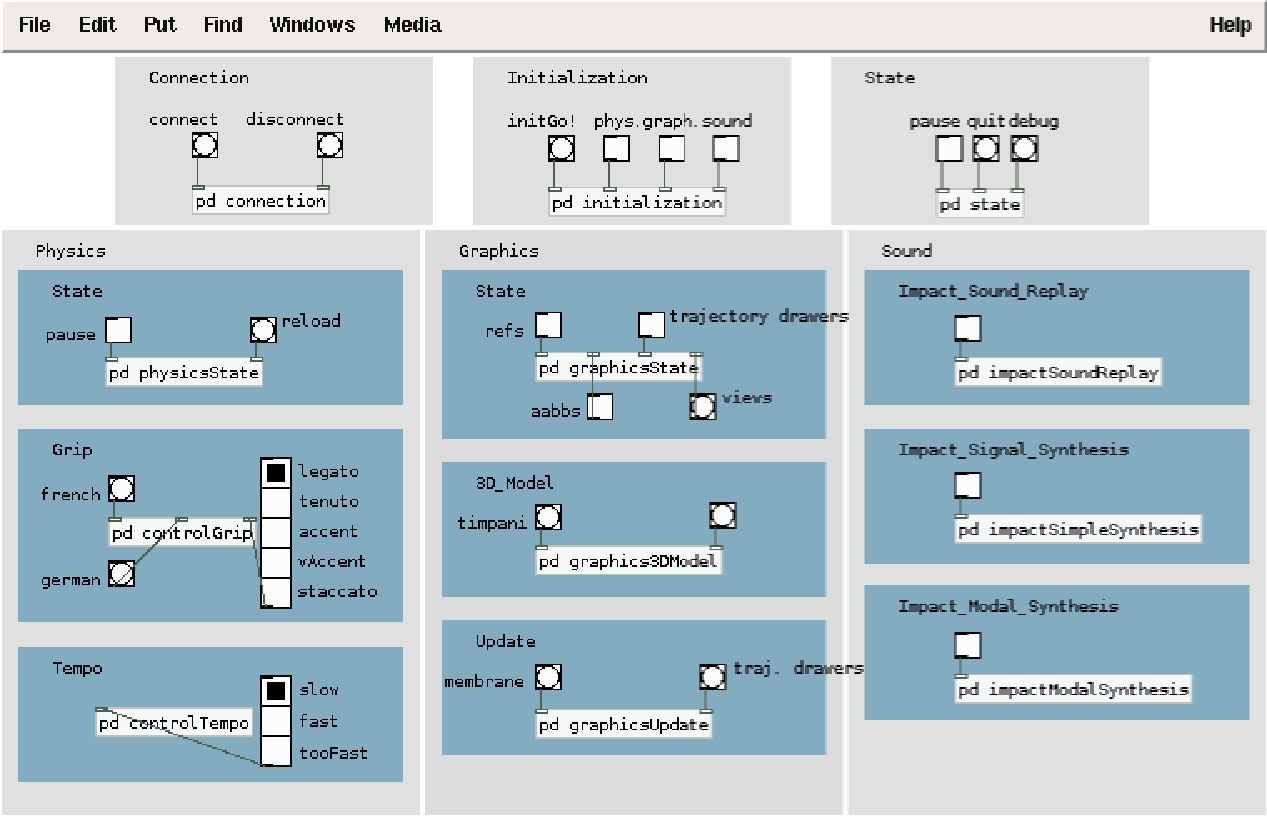
\includegraphics[width=0.8\linewidth]{Chapters/5/Pics/Pdf/userInterface.pdf}
%	\vspace{-0.5cm}
	\caption[User interface]{User interface: users can parameterize the percussion gesture to be simulated (drum grip, playing mode, tempo), as well as the graphics rendering and the sound feedback to be used (sound replay, signal-based and physically-based sound synthesis).}
	\label{fig:userInterface}
\end{figure}

Users can select different percussion grips (\emph{French} or \emph{German}), playing modes (\emph{legato}, \emph{tenuto}, \emph{accent}, \emph{vertical accent} and \emph{staccato}), and different tempi, to be simulated by the virtual percussionist. The parameterization of the visual and sound feedback is also possible. During the simulation, the interface provides users with different sound synthesis models such as the simple playback of sound clips, signal-based sound synthesis, or physics-based sound (modal) synthesis. Every sound synthesis technique proposed by the interface can be tuned in real time. For instance for the modal sound synthesis module, one can tune the parameterization of the drum membrane physics properties (radius size, mass, tension). The available sound and visual feedback is presented in \myfigname \ref{fig:visualFeedback}, which can be parameterized by users with the rendering of helpful visual cues such as mallet trajectories and beat impact locations of the drum membrane.

\begin{figure}[H]
	\begin{center}
		\subfigure[]{\label{fig:sim2}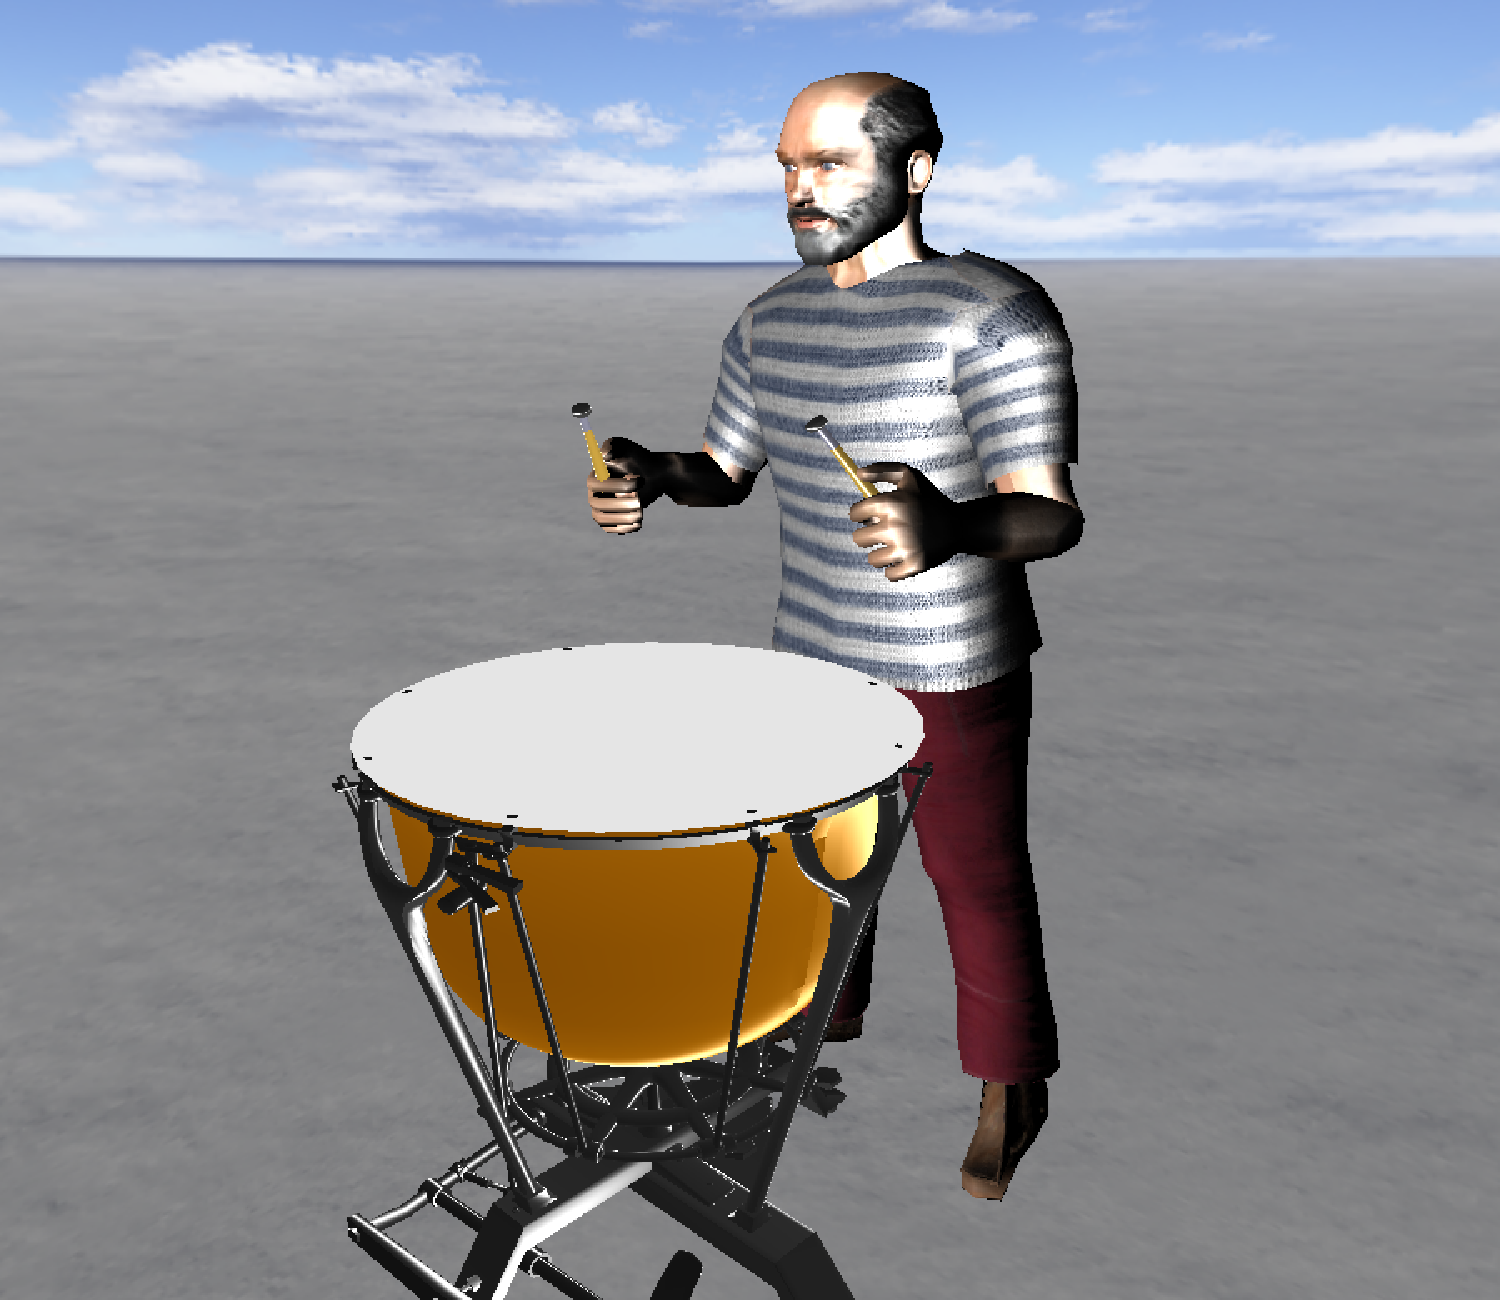
\includegraphics[width=0.3275\linewidth]{Chapters/5/Pics/Pdf/sim-gerard-1}}
		\subfigure[]{\label{fig:sim3}\includegraphics[width=0.3275\linewidth]{Chapters/5/Pics/Pdf/sim-gerard-2}}
		\subfigure[]{\label{fig:sim4}\includegraphics[width=0.3275\linewidth]{Chapters/5/Pics/Pdf/sim-gerard-3}}\\
		\subfigure[]{\label{fig:sim5}\includegraphics[width=0.9\linewidth]{Chapters/5/Pics/Pdf/simSound2}}\\
	\end{center}
	\vspace{-0.5cm}
	\caption[Visual feedback during the simulation]{Visual feedback during the simulation with (a) the final graphical model of the virtual percussionist. Users can explore and visualize the overall virtual percussion performance space, as well as (b) mallet trajectories and (c) beat impact locations. (d) Visual and sound renderings of beat impacts on the drum membrane.}
	\label{fig:visualFeedback}
\end{figure}

%%%%%%%%%%%%%%%%%%%%%%%%%%%%%%%%%%%%%%%%%%%%%%%%%%%%%%%%%%%%%%%%%%%%%%%%%%%%%%%%%%%%%%%%%%%%%%%%%%%%%%%%%%%%%%%%%%%%


%%%%%%%%%%%%%%%%%%%%%%%%%%%%%%%%%%%%%%%%%%%%%%%%%%%%%%%%%%%%%%%%%%%%%%%%%%%%%%%%%%%%%%%%%%%%%%%%%%%%%%%%%%%%%%%%%%%%

	\section{Conclusion}
	\label{sec:Synthesis_Conclusion}

We proposed in this chapter a physically-enabled environment in which a virtual percussionist can be physically controlled and interact with a physics-based sound synthesis model. The physics-based control from real percussion performances guarantees to maintain the main characteristics of human motion data while keeping the physical coherence of the interaction with the simulated instrument.

Furthermore, the hybrid control mode combining \emph{IK} and \emph{ID} controllers leads to a more intuitive and consistent way of editing the motion to be simulated only from mallet extremity trajectories, as regards to the analysis presented in chapter \ref{chapter:Analysis}. This control mode is especially shown to be more accurate than traditional solutions for physically tracking motion capture data. %One limitation of our contribution is however to focus only on upper-body (arms) motion, that does not take into account for instance balance strategies.

Moreover, the proposed asynchronous client-server architecture takes advantage of motion and sound physics formulations, generating in real-time virtual percussion performances that can be parameterized from the motion to the sound. The physical interaction of the virtual percussionist with a physics-based model of a timpani membrane is presented, leading to the control of a sound synthesis model from the actions (impacts) of the virtual percussionist. %It shoulde be noted that this model does not take into account the reaction of gestures as regards to the vibration of the drum membrane.

%Among the perspectives of such work is the improvement of the interaction between motion simulation and sound synthesis. This can involve the design of a more powerful collision detection module. If we consider the physical simulation of the instrument, it might be interesting to include mechanical interactions, such as hammered or plucked interactions, or even modeling the mechanical structure of a finger or a hand. We also plan to extend the mapping possibilities between gesture parameters and sound input parameters, and to develop efficient methods for editing percussion captured motion in the 3D Cartesian space.

%A possible avenue is also to evaluate the musical possibilities offered by our framework for composing novel percussion sequences.



%%%%%%%%%%%%%%%%%%%%%%%%%%%%%%%%%%%%%%%%%%%%%%%%%%%%%%%%%%%%%%%%%%%%%%%%%%%%%%%%%%%%%%%%%%%%%%%%%%%%%%%%%%%%%%%%%%%%




\chapter{Musical Application and Evaluation}
\markboth{Musical Application and Evaluation}{Musical Application and Evaluation}
\label{chapter:Application}


%%%%%%%%%%%%%%%%%%%%%%%%%%%%%%%%%%%%%%%%%%%%%%%%%%%%%%%%%%%%%%%%%%%%%%%%%%%%%%%%%%%%%%%%%%%%%%%%%%%%%%%%%%%%%%%%%%%%

%The increasing availability of software for creating real-time simulations of musical instrument sounds allows for the design of new visual and sounding media. Nevertheless, from a conceptual and pratical point of view, the question of how these new instruments can be controlled has rarely been addressed in the literature.  In this paper, we present and extensively evaluate a framework for the control of virtual percussion instruments by modeling and simulating virtual percussionists, based on a motion capture database and on a physically-based movement simulation environment. We also discuss the benefits and limitations of such an approach as a means of synthesizing new expressive percussion performances.\\
%The increasing availability of softwares for creating real-time simulations of musical instrument sounds allows for the design of new visual and sounding media. Such interfaces propose then novel musical interfaces that most of the time rely on firstly tracking user gestures and secondly relating it to sound synthesis processes. The ever growing use and availability of motion capture data therefore leads to challenges in managing high-dimensional motion data as well as reusing these latter in other instrumental situations from those recorded. Relating these motion data to sound processes constitutes also a difficulty when designing new musical interfaces.

%Our framework provides a conceptual and practical solution for synthesizing adaptative and realistic percussion performances. It gives also the possibility of exploring visually the resulting perfomances as well as exploring the mapping between the synthesized percussion gestures with sound processes.\\

In this chapter, we propose a composition process for synthesizing novel (\emph{i.e.} previously not recorded) virtual percussion performances, as well as its evaluation in a musical perspective. We namely present how new virtual percussion performances can be synthesized through the specification of scores at the gestural level, by the definition of gesture units that can be assembled and articulated. Furthermore, a musical evaluation of synthesized percussion exercises is conducted by submitting these latter to the evaluation of a professional percussionist.\\

The chapter is organized as follows. %We introduce firstly the motivation of our approach to the composition and synthesis of virtual percussion performances in section \ref{sec:Music_Introduction}.
Section \ref{sec:Music_Composition} presents the adopted approach to the composition of novel virtual percussion performances at the gestural level, based on the assembling and articulation of gesture units. Synthesized percussion exercises as well as their musical evaluation by a professional percussionist are then presented in section \ref{sec:Music_Evaluation}. Section \ref{sec:Music_AL} then extensively discusses the advantages and limitations of our approach as regards to its musical perspectives. Finally, section \ref{sec:Music_Conclusion} concludes this chapter with further perspectives.

%\vspace{1cm}

%%%%%%%%%%%%%%%%%%%%%%%%%%%%%%%%%%%%%%%%%%%%%%%%%%%%%%%%%%%%%%%%%%%%%%%%%%%%%%%%%%%%%%%%%%%%%%%%%%%%%%%%%%%%%%%%%%%%


%%%%%%%%%%%%%%%%%%%%%%%%%%%%%%%%%%%%%%%%%%%%%%%%%%%%%%%%%%%%%%%%%%%%%%%%%%%%%%%%%%%%%%%%%%%%%%%%%%%%%%%%%%%%%%%%%%%%

%\section{Introduction and Motivation}
%\label{sec:Music_Introduction}

%Digital music instruments have been widely studied during the past decades, focusing on the elaboration of new interfaces for controlling sound processes. The design of these new musical instruments rely fundamently on the input instrumental gesture they can track, that is the reason why one of the major issue of their use and initial stage design depends on the considered method which makes available these gestural informations. Motion capture systems (either sensor or camera-based) have therefore become a widespread technical solution for tracking the applied instrumental gesture. Such systems are also used for analysing performer gestures so that a good understanding of the considered instrumental gesture can lead to the identification of gesture parameters which will be used for the interaction with sound processes.

%Nevertheless, motion capture data intrinsically present several drawbacks. The recorded motion is dependent on the uniqueness of the interaction situation under study. The recorded situation is unique in the sense that it is difficult to extrapolate it to new instrumental situations. Moreover, especially when considering music performances, it is difficult to set up a reliable synchronization between the recorded motion and the sound process, particularly when no physical informations is available about a given recorded motion.\\

%Research projects have given a special attention to the design of new digital musical instruments and sound synthesis methods for building new musical and interactive interfaces \citeCM{cook:AK02, miranda:AR06}. Especially regarding percussion-related systems, an important research direction is the development of devices to track performer gestures for controlling sound synthesis processes \citeCM{kapur:JNMR03}. Despite the availability of various devices, the most accurate hardware for tracking percussive gestures remains camera tracking systems \citeCM{tindale:NIME05}. These systems offer an effective method for capturing, analyzing \citeIPA{dahl:AAA04} and virtually reconstructing the whole body of a performer, but they fall short in retrieving the dynamic aspects of playing techniques. Moreover, mapping the recorded motion to sound synthesis processes many times relies on non-intuitive multi-dimensional correspondences \citeCM{dobrian:NIME06}. Finally, with such methods it is also far from straightforward to go beyond the recorded data and reuse it to synthesize adaptive and realistic new performances.\\

%At the same time, developments in sound synthesis have given rise to various methods to generate percussive sounds. Specifically, physics-based synthesis of percussive sounds has involved the modeling of a hammer \citeCM{avanzini:ICMC01}, collisions and sliding excitations \citeCM{avanzini:SMC04}, and drum skins \citeCM{chuchacz:NIME07}. However, their main limitation seems to lie in the way they are controlled. Despite a few early attempts to approach this issue, it is still not clear how to formally relate these models to the excitation by a (real or virtual) performer instrumental gesture, even with the availability of relevant works on the study of percussion gestures \citeIPA{dahl:PhD05} and the design of new percussion controllers \citeCM{aimi:PhD06}. Only a few previous works have explored the  modeling of the equivalent gestures thanks to a slowly evolving mechanical model \citeCM{gibet:PhD87, gibet:ICMC88}, and then the simulation of an articulated arm hitting a vibrating membrane \citeCM{gibet:ICMC90}. More recent attempts to overcome this limitation include works involving the animation of virtual instrumentalists (or virtual models acting as instrumentalists) \citeCM{hanninen:ICMC96, lytle:SIGGRAPH01}, and the synthesis of sounds from rigid body simulations \citeCM{vanDenDoel:SIGGRAPH01, obrien:SCA02}.\\

%Our contribution adresses this issue and propose a framework, taking motion capture data as input, for reproducing recorded percussion performances and also for synthesizing new percussion exercises that were not recorded. It combines a motion capture database of varied percussion gestures and a physically-enabled environment for simulating percussion performances. Our framework provides a conceptual and practical solution for synthesizing adaptative and realistic percussion performances. It gives also the possibility of exploring visually the resulting perfomances as well as exploring the mapping between the synthesized percussion gestures with sound processes.\\

\begin{figure}%[H]
	\begin{center}
		\includegraphics[width=0.9\columnwidth]{Chapters/6/Pics/Pdf/globalFramework}
	\end{center}
	\vspace{-0.5cm}
	\caption{Global approach to the composition process of virtual percussion performances.}
	\label{fig:composition}
\end{figure}

%%%%%%%%%%%%%%%%%%%%%%%%%%%%%%%%%%%%%%%%%%%%%%%%%%%%%%%%%%%%%%%%%%%%%%%%%%%%%%%%%%%%%%%%%%%%%%%%%%%%%%%%%%%%%%%%%%%%


%%%%%%%%%%%%%%%%%%%%%%%%%%%%%%%%%%%%%%%%%%%%%%%%%%%%%%%%%%%%%%%%%%%%%%%%%%%%%%%%%%%%%%%%%%%%%%%%%%%%%%%%%%%%%%%%%%%%

	\section{Gesture Edition and Composition}
	\label{sec:Music_Composition}

The synthesis system presented in the previous chapter is used for creating novel percussion sequences from available motion data. We detail in this section the motivation and mechanisms involved during the edition of gesture scores that are simulated by our synthesis system. We consider this edition step as a first advance towards the composition of virtual music performances with our system.\\

The basis of the presented edition process is highly inspired from existing works in representing music-related materials. Since the beginning of the transcription of music performances, composers and performers have used the idea of representing sounds as independent and distinct events. The most obvious example of this idea is of course the transcription of notes on music scores. This event-based representation can be more or less suited depending on the considered music performance. For example, it is useful for representing sounds produced by instruments that involve distinct actions, such as striking or plucking. For other instruments involving continuous actions, such as a vibrating reed or bowing, such representation can also be useful by defining events with a start, an end, a state change. This is namely the approach that was adopted in the design of the widespread \emph{MIDI} protocol \citeCM{midi}.

Similarly, we define a set of events that can be used in our system for synthesizing percussion performances. However, the drastic difference from the previously detailed event representation is that our system uses the manipulation of elementary \emph{gesture events}. In fact, these gesture events are consituted of motion signals coming directly from motion data presented in chapter \ref{chapter:Analysis}. We will therefore refer to them as \emph{gesture units}. \myfigname \ref{fig:composition} depicts the use of these gesture units in our synthesis system. The edition and assembling of these canonical gesture units leads to the specification of a \emph{gesture score}, whose equivalent signal is then simulated by our system.

\begin{figure}%[H]
	\begin{center}
%		\subfigure[]{\label{fig:grips1}\includegraphics[width=0.325\columnwidth]{Chapters/6/Pics/Pdf/frenchGripUnitsCurves.pdf}}
%		\subfigure[]{\label{fig:grips1}\includegraphics[width=0.45\linewidth]{Chapters/6/Pics/Pdf/frenchGripUnits2.pdf}}
		\subfigure[]{\label{fig:grips1}\includegraphics[width=0.45\linewidth]{Chapters/6/Pics/Pdf/articulation1.pdf}}
		\hspace{6mm}
%		\subfigure[]{\label{fig:grips2}\includegraphics[width=0.325\columnwidth]{Chapters/6/Pics/Pdf/germanGripUnitsCurves.pdf}}
%		\subfigure[]{\label{fig:grips2}\includegraphics[width=0.45\linewidth]{Chapters/6/Pics/Pdf/germanGripUnits2.pdf}}
		\subfigure[]{\label{fig:grips1}\includegraphics[width=0.45\linewidth]{Chapters/6/Pics/Pdf/articulation2.pdf}}
	\end{center}
	\vspace{-0.5cm}
	\caption[Gesture edition and composition]{Gesture edition and composition: (a) \emph{beat-centered} gesture units for \emph{legato} (blue) and \emph{accent} (red) playing modes, (b) resulting simulation of the assembling of the two units.}
	\label{fig:FrenchGermanGrips_Sim}
\end{figure}
		
Our edition and composition process of gesture scores makes available gesture units of different types. These gesture units are directly related to the motion capture database, so that a huge amount of gesture units are available for representing the playing techniques under study (grips, playing modes, beat locations). We detail here how these gesture units are obtained, as well as how gesture scores are edited from these latter. This involves both an adequate segmentation of motion capture data, as well as an assembling (composition) of the resulting gesture units.\\

An interesting technical question here is the way the simulation step uses the edited gesture scores. The segmentation process discussed in section \ref{subsec:Analysis_TimpaniAnalysis_Segmentation} leads to \emph{beat-to-beat} gesture units for each of the playing techniques under study. It should be noted however that gesture scores involving such \emph{beat-to-beat} gesture units are not usable in a simulation context. This segmentation creates two types of problem. The first one is related to the fact that linking two gesture units at the moment of the beat impact may create unwanted kinematic discontinuities, concerning the position and orientation (and their derivatives) of both mallet extremities and body segments. Another problem that can occur is the alteration of beat impact profiles. Linking two gesture units at the beat impact would lead to separate impact profiles in two phases, which may results in the modification of the action/reaction mechanical nature of the impact. Finally, placing the articulation point between two gesture units during the beat impact disagrees with the usual decomposition of instrumental gestures into preparatory, interaction and retraction gestures.

%since it would imply that the articulation point between gesture units is achieved during beat impact contacts. This segmentation choice creates issues from a simulation point of view, since the end and start of two gesture units often show differences in position and orientation of the rigid bodies composing the virtual character. Managing the transition between two gesture units this way may create unwanted motion effects since the contact of the mallet with the drum membrane create external forces that act on these rigid bodies. Such transition during the contact with the drum membrane could also have a dramatical effect on the simulated beat impact. Furthermore, such transition disagrees with the usual decomposition of instrumental gestures into preparatory, interaction and retraction gestures.

We therefore translate gesture units from \emph{beat-to-beat} to \emph{beat-centered} units. Handling the articulation between gesture units in such a way is more consistent since the articulation point is placed between the retraction phase of the previous gesture unit and the preparatory phase of the next one. However, even such a unit representation may lead to discontinuities in position and velocity between two gesture units. That is why we ensure a C$^1$ continuity on drumstick extremity trajectories. Examples of \emph{beat-centered} gesture units for \emph{legato} and \emph{accent} playing modes are presented in \myfigname \ref{fig:FrenchGermanGrips_Sim}, with the corresponding simulation of the assembling of the two units.\\

Another issue to discuss concerning the edition of gesture scores is the way the gesture units are assembled to create a partition that our system will simulate. This includes two underlying questions, on the one hand which gesture unit will be chosen for representing a playing technique since many units are available, and on the other hand how the assembling is practically achieved?

The equivalent problem to the first question brings back, for a given playing technique, to the existence of a "best-suited" gesture unit among the available ones. This issue has also been under study in \citeCM{ramstein:PhD91} concerning piano fingering. Our viewpoint on this open question is to argue that performers are highly trained to replicate and adapt their  gestures under a wide range of conditions. So that our solution is to pick up a particular gesture unit in a captured sequence, apart from the first and last one. This restriction ensures that no external disturbance is included in the gesture unit, as it was observed that performers tend to test the balance of their mallets at the beginning of a sequence, and exaggerate their motion when finishing it.

Once a set of gesture units is available for representing each playing technique, a strategy has to be developped for assembling these in a whole coherent gesture score. This includes again two underlying problems. The first one concerns the articulation between different position and orientation postures of the virtual character from the end of a gesture unit to the beginning of the next one. In all the percussion exercises presented in this chapter, this problem was achieved mainly by focusing only on the mallet extremity trajectories, as these latter are essential factors in percussion gestures as underlined in chapter \ref{chapter:Analysis}. The choice of the gesture units was therefore achieved by a careful analysis of the height of mallet extremity trajectories so that a match can be found between the end of a gesture unit and the beginning of the next one. The animation engine then involves an interpolation process for transitioning from a gesture unit to another. The second problem concerns the timing issue when mixing heterogenous gesture units. It has been easily overcome due to the high proficiency of performers in keeping a steady tempo.

%sketching, issue: position, orientation => interpolation; timing

%Another limiting issue is the choice of the gesture units used during the editing step. Such issue yields inevitably to the question of the existence of a best-suited gesture unit, compared to other examples of the same playing mode. If such "best" gesture unit exists, how can one identify it among the numerous replicates available in the motion database? Otherwise, does it make sense to average multiple gesture units so that a "mean" gesture unit can be used? We believe that using an average gesture might lead to the loss of some expressive features implicitly contained in the gesture signal. We therefore chose one specific gesture example within the sequence, without trying to find an optimized criteria for selecting this gesture unit. %[Can you comment on the consequences of this arbitrary choice?]


%%%%%%%%%%%%%%%%%%%%%%%%%%%%%%%%%%%%%%%%%%%%%%%%%%%%%%%%%%%%%%%%%%%%%%%%%%%%%%%%%%%%%%%%%%%%%%%%%%%%%%%%%%%%%%%%%%%%


%%%%%%%%%%%%%%%%%%%%%%%%%%%%%%%%%%%%%%%%%%%%%%%%%%%%%%%%%%%%%%%%%%%%%%%%%%%%%%%%%%%%%%%%%%%%%%%%%%%%%%%%%%%%%%%%%%%%

	\section{Musical Evaluation of Virtual Percussion Performances}
	\label{sec:Music_Evaluation}

One of the most interesting outcomes of such framework is the possibility of handling and assembling heterogeneous performances using a combination of a few percussion gesture units. Thanks to the physics simulation of the virtual performer, the issue of gesture articulation between movement units is partly addressed by the physics engine, thus leading to a more natural sequence of movements\footnote{The resulting articulation is not necessarily equivalent to real performer techniques. It will nevertheless be a physically plausible solution to the problem.}.\\

\begin{table}%[H]
	\centering
	\caption{Timpani playing notation}
	\begin{tabular}{||x{2.3cm}|x{2.3cm}|x{2.3cm}|x{2.3cm}|x{2.3cm}||} \hline
		\small{$Legato$} & \small{$Tenuto$} & \small{$Accent$} & \small{$V.Accent$} & \small{$Staccato$}		\tabularnewline \hline \hline
		\includegraphics[height=10.8mm]{Chapters/6/Pics/Pdf/legato} & \includegraphics[height=16mm]{Chapters/6/Pics/Pdf/tenuto} & \includegraphics[height=14.1mm]{Chapters/6/Pics/Pdf/accent} & \includegraphics[height=15.2mm]{Chapters/6/Pics/Pdf/verticalaccent} & \includegraphics[height=15.5mm]{Chapters/6/Pics/Pdf/staccato} 	\tabularnewline \hline \hline
		\small{$One-Third$} & \small{$Center$} & \small{$Rim$} & \small{$Left$} & \small{$Right$}		\tabularnewline \hline \hline
		\includegraphics[height=15.5mm]{Chapters/6/Pics/Pdf/onethirdlocation} & \includegraphics[height=15.5mm]{Chapters/6/Pics/Pdf/centerlocation} & \includegraphics[height=15.5mm]{Chapters/6/Pics/Pdf/rimlocation} & \includegraphics[height=13.8mm]{Chapters/6/Pics/Pdf/leftbeat} & \includegraphics[height=13.8mm]{Chapters/6/Pics/Pdf/rightbeat} 	\tabularnewline \hline
	\end{tabular}
	\label{tab:notation}
\end{table}

To evaluate the proposed framework, we have simulated an extensive set of musical examples consisting of several timpani exercises\footnote{The exercises presented in this chapter are available at\\ \href{http://www-valoria.univ-ubs.fr/Alexandre.Bouenard/index.php/Research/PhDThesis}{http://www-valoria.univ-ubs.fr/Alexandre.Bouenard/index.php/Research/PhDThesis}}. The resulting simulations were evaluated by the last author (a University Percussion Professor and an active Performer)\footnote{Prof. F. Marandola (Schulich School of Music, McGill University) has chosen the percussion exercises to be simulated by the virtual character. He also qualitatively evaluated the synthesized percussion exercises.}, by focusing both on the visual and auditory feedback, first simultaneously and then separately. The exercises are divided in two main categories: validation and extrapolation exercises.\\

The first category, validation exercises, aims at verifying the accuracy with which the proposed framework can synthesize percussion movements (and sounds) similar to the captured movements in the database. They consist in independent exercises that explore variations on the type of grip (\emph{French} or \emph{German}), the type of playing mode (\emph{legato}, \emph{tenuto}, \emph{accent}, \emph{vertical accent} and \emph{staccato}), as well as the position of the impact on the drum membrane (one-third, center or rim).\\

The second category, extrapolation exercises, consist in musical excerpts that go beyond those obtained with motion capture. Such exercises were not performed by the musicians and therefore no articulation data corresponding to these exercises are available. They typically mix various types of gestures and impact positions in one excerpt, as well as variations on the tempo of the performances.\\

Throughout this section, all percussion exercises exploit gesture units in the motion capture database described in section \ref{sec:Analysis_MoCapDatabase}. The notation corresponding to timpani playing techniques is described in \mytabname \ref{tab:notation}, and is used as the standard notation throughout the rest of this paper for describing percussion exercise scores.


		\subsection{General Comments}
		\label{subsec:Music_Evaluation_GeneralCommments}

Although the simulations look and sound realistic, a first musical evaluation was achieved for determining the overall degree of expertise of the virtual performer. From the resulting simulations, we can see that the virtual timpanist's performance is similar to that of a beginner/intermediate performer.
Only part of the attacks were performed correctly, but with a wide range of variation in the impact locations and in the motion of the arm and forearm.
Other issues in the simulations include the fact that the grip is not as realistic as expected. Moreover, the bottom part of the virtual character's body does not move. This fact may be of little importance for a set of repeated notes at a steady tempo, but becomes more significant when variations in location, intensity, types of attack and rhythm occur.\\

The setup described in section \ref{sec:Analysis_MoCapDatabase} actually does not include the recording of the subtleties occurring in the mallet grips, since no sensors are monitoring the grasp mechanisms involving the fingers and the mallets. Although our motion capture setup does capture the orientation of hands and mallets, this information is not sufficient for modeling the grasp subtleties that could enhance the realism of the resulting grip simulations. Furthermore, no balance strategies are involved in the simulation of the percussion exercises, although information on performers' center of mass was captured in the motion capture sessions. This simulation choice explains the remark on the quite static bottom part of the virtual performer.


		\subsection{Validation Exercises}
		\label{subsec:Music_Evaluation_Validation}

In this section we analyze how the system manages to connect independent gesture units taken from the timpani database, where each exercise consists in a sequence of similar types of strokes. The strokes are chosen from pre-selected gesture units, corresponding to a given grip, a playing mode and a location on the timpani.
We focus on the qualitative evaluation of the simulation of playing modes as well as beat impact locations\footnote{The simulation quality of \emph{French} or \emph{German} grips is further discussed in section \ref{subsubsec:AL_IGS_L}. }.

We simulated five exercises consisting of 13 strokes each (7 for the right hand and 6 for the left hand) for each playing mode. \myfigname \ref{fig:validation1} shows an example of an exercise consisting only of \emph{legato} strokes, whereas \myfigname \ref{fig:validation2} shows the simulation score of beat impacts locations at the rim of the timpani membrane.\\

\begin{figure}%[H]
	\begin{center}
		\subfigure[]{\label{fig:validation1}\includegraphics[width=52mm]{Chapters/6/Pics/Pdf/exo1-1.pdf}}
		\hspace{1cm}
		\subfigure[]{\label{fig:validation2}\includegraphics[width=52mm]{Chapters/6/Pics/Pdf/exo5-3.pdf}}
	\end{center}
	\vspace{-0.5cm}
	\caption[Simulated exercises: validation of playing modes and impact locations]{(a) Simulation exercise consisting of a sequence of \emph{legato} strokes. (b) Simulation exercise consisting of a sequence of \emph{legato} strokes played at the rim.}
	\label{fig:gesture}
\end{figure}

As expected, the resulting simulations show significant variations in the quality of the attacks for a given type of stroke, specifically with respect to the location of the impact point. However, the shoulders present very large movements; there is an excessive shoulder rotation for each single stroke, making the position of the elbows not accurate. In fact, given the steady position of the bottom part of the body, there should be more motion at the elbows.

The exaggeration in shoulder and elbow movements can be attributed to the physical model of the virtual percussionist. Just as any physical entity, the body parts of the virtual percussionist are characterized by inertia properties. When the physical model is put into motion, these body parts seem to acquire too much inertia, so that even if the overall motion (mallet extremities) is accurate enough compared to the recorded gesture units \cite{bouenard:AAA09}, an exaggeration of motion appears.\\

Considering only the sound generated, one can notice that the sound outcome is plausible and that playing modes producing them are audibly perceptible. However, the sound starts with too much attack (there is even some saturation at the beginning of the sound) and the resonance differs from a real timpani sound. Finally, the sound is not metallic enough when considering the attacks near the rim of the membrane.

These issues concern the \emph{Modalys} model of the drum membrane. The lack of sound resonance is easily explained by the fact that the drum membrane model does not feature a resonance body. Moreover, the non-metallic nature of the resulting sounds may also come from a combination of imprecisions both from the drum membrane model itself since no metallic rim is included in the \emph{Modalys} model, and from beat impact locations inaccuracies.


		\subsection{Extrapolation Exercises}
		\label{subsec:Music_Evaluation_Extrapolation}

The previous exercises consisted of simple sequences of similar strokes. Much more interesting though is to verify how the framework can deal with gestures combinations of different stroke types, tempos, and impact locations that were not initially recorded in sequence. Various combinations of gestures will be analyzed in the following subsections.


			\subsubsection{Playing Modes}
			\label{subsubsec:Music_Evaluation_Extrapolation_GestureVariations}
		
The following two exercises show a combination of gesture units for various playing modes. The idea is to show that the system can connect independent gesture units of each playing mode, as well as creating the articulation for a combination of these different units.

\begin{figure}%[H]
	\begin{center}
		\subfigure[]{\label{fig:gesture1}\includegraphics[width=82mm]{Chapters/6/Pics/Pdf/exo2-1.pdf}}
		\hspace{0.5cm}
		\subfigure[]{\label{fig:gesture2}\includegraphics[width=51mm]{Chapters/6/Pics/Pdf/exo4-5.pdf}}
	\end{center}
	\vspace{-0.5cm}
	\caption[Simulated exercises: extrapolation of playing modes]{(a) Simulation exercise consisting of five gesture units repeated four times: \emph{staccato}, \emph{legato}, \emph{tenuto}, \emph{accent} and \emph{vertical accent}, respectively. (b) Simulation exercise consisting of variations between \emph{legato} and \emph{accent} strokes, ending with a \emph{vertical accent}.}
	\label{fig:gesture}
\end{figure}

The first exercise (\myfigname \ref{fig:gesture1}) is a sequence of several strokes (respectively \emph{staccato}, \emph{legato}, \emph{tenuto}\emph{accent} and \emph{vertical accent}) in groups of four strokes (two per arm). The second exercise (\myfigname \ref{fig:gesture2}) changes the type of stroke for each arm from \emph{legato} to \emph{accent} and back, finishing with a \emph{vertical accent} performed with the right hand.\\
		
Considering the articulation between the simulated playing modes, it can be seen that articulation changes are perceptible throughout the simulation. However, problems arise in \emph{legato}-\emph{tenuto} and \emph{tenuto}-\emph{accent} pairs, so that differences between these are sometimes not very clear. These can be the result of the motion exageration discussed previously (cf. section \ref{subsec:Music_Evaluation_Validation}), as well as from the fact that the effect of fingers is not available in the recorded motion data (cf. section \ref{subsec:Music_Evaluation_GeneralCommments}).

%[This may be a bit too detailed for the CMJ paper]

%For the first pair of strokes, the over motion of the shoulder in the \emph{legato} stroke masks partially the difference with the \emph{tenuto} strokes. For the second pair (\emph{tenuto-accent}), the phenomenon occurring around the fulcrum (between the thumb and the index), characterized by a change of pressure, is not perceptible, it is indeed of utmost importance to help to bring out the sharpness of the attack. 

%Again, the interpretation of the phenomena pointed out by the percussion professor comes, on the one hand, from the motion exaggeration discussed previously (cf. section \ref{subsec:validation}), and on the other hand from the fact that the effect of fingers is not available in the recorded motion data (cf. section \ref{subsec:general_commments}).\\

%As for the recognition of gesture variations from the simulated sounds, it was noted that although variation in the impact location is important throughout the exercise between \emph{legato} and \emph{accent} strokes, this variation was limited here: %[Is this right???] 
%all the \emph{legato} strokes are performed closer to the center, what helps to bring out a difference in the timbre (attack and resonance). However, these variations are too important to be able to distinguish only by listening the exact alternation of \emph{legato} and \emph{accent} strokes. % [Is there variation in the simulation or not? I am lost here!]

The resulting sounds from the articulation between various playing modes were perceptible, except for the \emph{legato}-\emph{accent} sequences. This lack may result from both the \emph{Modalys} model of the drum membrane and from the simulated articulation problem in this case as pointed out previously.


			\subsubsection{Tempo Variations}
			\label{subsubsec:Music_Evaluation_Extrapolation_TempoVariations}

We have tested the simulation of articulating the same percussion gesture (\emph{legato}) under an accelerando-decelerando musical variation\footnote{This tempo variation has not been recorded initially.}. \myfigname \ref{fig:tempo1} shows the percussion exercise simulated by the virtual percussionist. 

\begin{figure}%[H]
	\begin{center}
		\subfigure[]{\label{fig:tempo1}\includegraphics[width=60mm]{Chapters/6/Pics/Pdf/exo3-1.pdf}}\\
%		\hspace{1cm}
		\subfigure[]{\label{fig:tempo2}\includegraphics[width=\linewidth]{Chapters/6/Pics/Pdf/accelerandoDecelerando4.pdf}}
	\end{center}
	\vspace{-0.5cm}
	\caption[Simulated exercises: extrapolation of tempo variations]{(a) Simulation exercise consisting of an accelerando followed by a decelerando of \emph{legato} strokes. Note that the timpani mocap database only has samples of \emph{legato} strokes capture at one given tempo. (b) Simulation and articulation between \emph{legato} beats under an accelerando-decelerando musical variation (height of the tip of the mallet). %The top arrow shows an amplitude increase occurring during the accelerando, as well as small amplitude drop when approaching the maximum accelerando velocity.
}
	\label{fig:tempo}
\end{figure}

Regarding the quality of the synthesized \emph{legato} strokes under such tempo variation, it can be seen in the simulation that the motion of the shoulders increase with the speed (becoming way too wide), while the amplitude of the motion of the forearms and the space between them remain identical. In reality, timpanists would have a tendency to bring closer their forearms and to reduce the amplitude of the vertical movements of the forearms and mallets, compensating by increasing the motion of the wrists and an increased use of the fingers. Moreover, during this accelerando phase, the flow becomes more irregular and the impact locations substantially change, causing inconsistency in the quality of the sounds produced. 

%Once again, this result would be consistent with that of a beginner who would partially lose control of his motion with the increases in performance speed.
%[Maybe keep this for the conclusions?]

\myfigname \ref{fig:tempo2} displays the motion amplitude increase (mallet extremity) along the accelerando-decelerando exercise shown in \myfigname \ref{fig:tempo1}. This increase can be explained by a gain of inertia in the physical model of the virtual percussionist (cf. section \ref{subsec:Music_Evaluation_Validation}). %More interestingly, there is also an amplitude drop in the vertical motion of the mallet extremity when approaching the maximum velocity of the accelerando (see the arrow in \myfigname \ref{fig:tempo2}). This phenomenon does agree with the expected amplitude decrease expected in real performances. However, this natural amplitude drop combined with an unwanted increase of motion does not seem to be visually and auditory perceptible.

The inconsistency reported on beat impact locations can be explained from a simulation point of view. As mentioned in section \ref{subsec:Synthesis_Physics_MotionControl_CartesianSpaceControl} and emphasized by equation \ref{eq:equation3}, the control of the virtual percussionist is achieved by the control of errors between target and state mallet extremities. The accelerando phase seems to have a critical effect on the control of such errors, leading to the propagation of joint errors on the mallet extremity and on beat impact locations.\\

As for the quality of the corresponding synthesized sounds to this percussion exercise, during the accelerando, a crescendo occurs naturally by setting on resonance the membrane of timpani. It should be noticed that this feature is also used by real timpanists to build-up a crescendo during a roll: they increase the speed of their rolls to build up the crescendo while they tend to find the speed which brings out the maximum natural resonance from the timpani.

This fact attests to the natural response of the \emph{Modalys} model of the drum membrane in response to the simulated \emph{legato} strokes under an accelerando tempo variation. It shows moreover that the interaction model, and especially the collision detection of beat impacts, offers realistic features such as contact durations and forces in comparison to real timpani performances.


			\subsubsection{Impact Location Variations}
			\label{subsubsec:Music_Evaluation_Extrapolation_ImpactVariations}

\begin{figure}%[hd]
	\begin{center}
		\includegraphics[width=130mm]{Chapters/6/Pics/Pdf/exo7-1.pdf}
	\end{center}
	\vspace{-0.5cm}
	\caption[Simulated exercises: extrapolation of impact location variations]{Simulation exercise consisting of several \emph{legato} strokes played at various locations in the membrane (o: one-third, c: center and r: rim).}
	\label{fig:exo7-1}
\end{figure}

Finally, we simulated the exercise depicted in \myfigname \ref{fig:exo7-1}, consisting in a sequence of several \emph{legato} strokes played at various beat impact locations. This exercise aims to verify if the articulation of various beat impact locations results in still perceptible changes in the simulation.

In fact, the differences remain perceptible, more specifically with respect to the end of the exercise (two last groups of four strokes: o c o r). However, one would expect that the differences would be more obvious among the three types of location, specifically for the centered strokes. 

The reason for this effect is that the original recorded performances that were used to build and simulate this exercise were not performed accurately enough with respect to impact position. As shown in \myfigname \ref{fig:variability}, the recorded beat impact locations (hollow signs) for the center location are too near to those corresponding to the one-third location.

%The comments underline the articulation quality between the selected gesture units for simulating different beat impact locations, and especially for the difficult task of simulating one-third, center and rim beat impact locations in a short time lapse ("o c o r"). Moreover, the percussion professor hypothesizes that the difficulty in discriminating center locations can be due to the captured gesture units used for the composition and simulation of the exercise. This hypothesis do agree with the observation of beat impact locations initially recorded. 

%%%%%%%%%%%%%%%%%%%%%%%%%%%%%%%%%%%%%%%%%%%%%%%%%%%%%%%%%%%%%%%%%%%%%%%%%%%%%%%%%%%%%%%%%%%%%%%%%%%%%%%%%%%%%%%%%%%%


%%%%%%%%%%%%%%%%%%%%%%%%%%%%%%%%%%%%%%%%%%%%%%%%%%%%%%%%%%%%%%%%%%%%%%%%%%%%%%%%%%%%%%%%%%%%%%%%%%%%%%%%%%%%%%%%%%%%
		
	\section{Discussion: Advantages and Limitations}
	\label{sec:Music_AL}

Simulating instrumental percussion gestures for controlling sound synthesis processes presents advantages and limitations, and these are of different orders when considering each module of our framework. In the following sections we will analyze in detail some of the sources of variability that are produced by our simulation system and may be at the origin of unwanted artifacts, as well as new interesting possibilities. We therefore consider sequentially the advantages and limitations of each module of our framework, considering first the instrumental gesture simulation and then the gesture edition step (cf. \myfigname \ref{fig:composition}).


		\subsection{Instrumental Gesture Simulation}
		\label{subsec:Music_AL_IGS}

We here underline the importance of the parameterization of the virtual character during the simulation. A non-optimal parameterization can lead to artifacts in the resulting synthesis of percussion performances, as well as to effects on synthesized sounds. We also highlight the interest of simulating instrumental gestures with respect to the possible modulation of synthesized gestures while preserving the initial style and expressive characteristics of real percussion performances.


			\subsubsection{Advantages}
			\label{subsubsec:AL_IGS_A}

From a simulation point of view, once an acceptable parameterization of the simulation is achieved, associating a motion capture database and the physics-based synthesis of instrumental gestures yields an accurate simulation of movements.

\begin{figure}%[H]
	\begin{center}
		\includegraphics[width=0.8\columnwidth]{Chapters/6/Pics/Pdf/beatImpactsAnalysis2.pdf}
	\end{center}
	\vspace{-0.5cm}
	\caption[Comparison of captured and simulated beat impact locations played \emph{legato}]{Comparison of captured and simulated beat impact locations played \emph{legato}. Small hollow signs represent strokes from motion capture data, whereas large hollow signs represent beat impact locations resulting from the chosen gesture units. Bold signs represent the simulated beat impact locations.}
	\label{fig:variability}
\end{figure}
	
A first advantage of the our physics-based framework for simulating percussion gestures is the retrieval of the dynamical aspects (beat impacts) of the recorded instrumental gestures, since no extra sensors have been used during the recording of percussion performances and no information concerning beat impact durations and forces has been recorded. Such physical approach is also of great interest for exploring the interaction of percussion gestures with sound synthesis since it makes available useful contact information that can be exploited by sound synthesis processes.

A second advantage of our system is its virtual nature. Indeed, the proposed framework allows the modeling of realistic phenomena occurring during real percussion performances. Furthermore, it also allows to go beyond reality, and provides the possibility of modifying the parameters of the virtual environment as wanted for creating new percussion performances. Among these parameters, it includes modifications of the physical model of the virtual percussionist, leading for instance to various stiffness properties of the synthesized gestures. Different interaction schemes between synthesized gestures and sound synthesis inputs can also be explored.\\

From a more musical point of view, an issue to take into account is the small variations in movements that are important to produce expressive performances. Indeed, deadpan performances where movements are kept as close to an ideal movement target as possible are considered mechanical and non expressive. By choosing a single gesture unit for representing each playing mode in the various simulations, we might actually expect to eliminate the natural variability of movements from the original performance by the (real) percussionists. This choice, although greatly simplifying the simulation, has the downside of potentially creating mechanical performances.

Nevertheless, thanks to the physics simulation layer, departing from a single gesture unit for each gesture type will nevertheless produce synthesized gestures with inherent variability due to the dynamic characteristic of the virtual character. This micro variability can be explained by a combination of effects occurring at each level of our framework. As explained below, for the instrumental gesture simulation, numerical drifts can occur but still be controlled. Exploiting such drifts for slightly modifying the instrumental gesture may produce some form of expressiveness. For instance, single simulations of the same gesture unit yield slightly different yet consistent synthesized gesture units, as shown in \myfigname \ref{fig:FrenchGermanGrips_Sim}. The propagation (and not the amplification) of such numerical drifts is also influenced by the edition and the articulation of gesture units, thus leading to another source of variability during the simulation of a sequence of several gesture units. These small differences in gestural trajectories therefore lead to variations in the impact locations on the membrane, thus producing variations in corresponding synthesized sound. These different effects may be explored musically, and actually lead to non-mechanical performances by the virtual percussionist.

An example is presented in \myfigname \ref{fig:variability}, showing the simulation of several \emph{legato} strokes for the \emph{French} grip. Small hollow signs represent the 2D positions of motion captured strokes on the drum membrane respectively for the three impact positions. The three large hollow signs indicate the impact positions of the three captured strokes chosen as gesture units for each hand. Finally, the bold signs represent the various simulated strokes. One can note the comparable variability of the (real) percussionist's strokes from motion capture (small hollow signs), and the resulting variability of the synthesized strokes (small bold signs) from multiple simulations of each gesture unit.


			\subsubsection{Limitations}
			\label{subsubsec:AL_IGS_L}

Depending on the sequence and speed of the selected gestures, as well as to the fine tuning of the mechanical joints (equation \ref{eq:equation3}), simulation artifacts can appear and result in large variations in beat impact positions and forces. These variations are due to the adaptation of the physics simulation to the constraints in the movement data, and may yield unexpected sound phenomena.\\

An example is presented in \myfigname \ref{fig:soundComparison}, where the virtual musician performs a sequence of four beats played \emph{legato} with different sets of physical constraints (mechanical joints). In \myfigname \ref{fig:soundComparison1}, a simulation artifact can be observed on the third beat, that results in a larger sound waveform amplitude and sound intensity, actually masking the last beat. This artifact is removed by changing the physics constraints expressed by the damping and stiffness coefficients involved in equation \ref{eq:equation3}, as shown in \myfigname \ref{fig:soundComparison2}. In this latter case, one can see that the four beats are performed similarly, both in terms of amplitude and intensity\footnote{Sounds in both simulations have been obtained using \emph{Modalys}.}.

The parameterization of the mass and density of the different segments composing the physical model of the virtual percussionist should be chosen carefully, so that the inertial behavior of the system is comparable to that of humans. Otherwise accelerations or slowdowns as well as unexpected overruns may be obtained, leading to unrealistic simulations.

\begin{figure}[H]
	\begin{center}
		\subfigure[]{\label{fig:soundComparison1}\includegraphics[width=0.4\linewidth]{Chapters/6/Pics/Pdf/soundComparison_waveAmplitude_1.pdf}}
		\hspace{6mm}
		\subfigure[]{\label{fig:soundComparison2}\includegraphics[width=0.4\linewidth]{Chapters/6/Pics/Pdf/soundComparison_waveAmplitude_2.pdf}}\\
		\subfigure[]{\label{fig:soundComparison3}\includegraphics[width=0.4\linewidth]{Chapters/6/Pics/Pdf/soundComparison_waveAmplitude_3.pdf}}
	\end{center}
	\vspace{-0.5cm}
	\caption[Instrumental gesture simulation: artifacts and their influence on sound synthesis]{(a) A simulation artifact causes much larger sound waveform amplitude and sound intensity on the third beat, compared to (b) a stable simulation generating fairly constant amplitude and intensity for all beats. (c) Issues (1) and (2) discussed below: (1) artifact when two close beat impacts are glued together by the sound synthesis engine to form a huge sound, and issue (2) when two close beat impacts are finally heard.}
	\label{fig:soundComparison}
\end{figure}

Moreover, variations in the simulations of the two percussion grips can be found in the assembly of more complex gesture sequences. \emph{French} grip simulations work well, due to the large flexibility and smoothness of movement which lead to large amplitudes in the trajectories deployed by the human performer (cf. \myfigname \ref{fig:grips1}). The simulation framework is capable of following the original gesture trajectories and can articulate the sequence of gestures. For the \emph{German} grip though, due to the large motion-phase where the performer keeps the mallet relatively immobilized close to the membrane, the physics engine results are less satisfactory. This is mostly seen in sequences of gestures assembled from gesture units. The less successful simulation of \emph{German} grip can be due to two reasons.

The first reason is that our motion data does not take into account the fact that expert percussionists commonly use their fingers to help performing the strokes. This is true for both \emph{French} and \emph{German} grips, but the effect of this technique in the \emph{German} grip can be more important. The use of the \emph{German} grip involves generally a technique requiring more control from the wrist and fingers and less amplitude of the arms and forearms, in order to control the speed of the mallet as well as the duration of contact between the mallet and the timpani membrane.

The second reason reveals the fact that the mallets (and therefore the percussionists' arms) stay relatively immobile during a large portion of the gesture unit (cf. \myfigname \ref{fig:classifParameters}). It necessitates the simulation of fixed and more rigid postures that especially involve the tuning of the physical parameters with high stiffness values, thus potentially leading to instabilities in the numerical simulation. 
		
\myfigname \ref{fig:soundComparison3} shows the effect of this issue on the resulting sound. The virtual performer is given a task to perform a sequence of \emph{accent} strokes using captured data of the \emph{German} grip. From the resulting sounds, one can notice that at some moments, {\it (1)} the sound amplitude is largely superior to the average, and {\it (2)} the resulting beats are not regularly spaced, although no dynamics or tempo variation was present in the score. Issue {\it (1)} characterizes a larger stroke seen in the figure as an artifact from the sound synthesis generation, \emph{i.e.} the simulated gesture presents strokes that are very close temporally and spatially. The collision detection events, performed in a short lapse time, are then interpreted by the \emph{Modalys} system which "glues" them together as a single yet much stronger stroke. As for issue {\it (2)}, it can be explained by the limitations of both the capture database and the simulation framework, as discussed above. 


		\subsection{Motion Database and Gesture Edition}

Our framework depends highly on the motion clips initially recorded during the acquisition process of motion data. The motion database associated with edition processes are off-line components that are of particular importance when considering the composition of a gesture score. In this section we examine the assets and drawbacks of our system with respect to these components. We initially highlight the advantages of our framework in considering the simulation of percussion performances at the gestural level. We then discuss the completeness of the available motion capture database, as well as the editing method presented in this paper.


			\subsubsection{Advantages}

In this work, we adopted a sketching approach to the composition of gesture scores made of elementary gesture units. This constitutes an intuitive process where the user only needs to select and assemble a limited amount of canonical gesture units, one for representing each timpani playing mode. The gesture score can then be seen as copy-and-paste and concatenation processes of these gesture units to form a whole gesture score.\\

Although the presented model does not take into account the subtle articulation mechanisms occurring in real percussion performances, a simple articulation (interpolation) of gesture units is implicitly achieved by the internal physics simulation when the gesture score simulation switches from a gesture unit to another. Such a "sketching" approach has the advantage to be transparent to the user.\\

Another advantage of our framework in considering the composition at the gestural level is the preservation of the expressive features inherent to real percussion performances. As the composition process of gesture scores relies highly on real motion data, this insures that simulations will preserve the expressive components of the gesture units used in the gesture score. More interestingly, it allows consequently to preserve the style of the real performer in the simulated percussion performances. Specifically in this work, all the exercises presented in section \ref{sec:Music_Evaluation} have used motion data from one performer, such that these simulated exercises can be considered as supplementary exercises that we might have asked the percussionist to perform.\\

The presented motion capture database in section \ref{sec:Analysis_MoCapDatabase} focuses on a particular excerpt (grip, playing mode and beat location) among the multitude of percussion techniques used by timpani performers. Our system provides the interesting possibility of enriching this limited database by the editing and simulation of novel percussion performances. One can also consider our approach as a means of preventing the tedious and time-consuming task of capturing an exhaustive motion database containing all the possible combinations of playing techniques. %More specifically about the capture of music performances, such an approach prevents also from the worrying task of elaborating complex capturing settings to synchronize motion and sound data thanks to the physics-based framework. 
Finally, our framework provides an interactive tool that can be used in the exploration of the relationship between instrumental gestures and sound processes.


			\subsubsection{Limitations}

The motion capture database presented in section \ref{sec:Analysis_MoCapDatabase} focuses on specific set of timpani playing techniques, i.e. it provides gesture examples only for these playing techniques. As seen before, this fact limits the possible simulations to be performed with the proposed system.\\

Another limiting issue is the choice of the gesture units used during the editing step. As already discussed in the beginning of this chapter, such issue yields inevitably to the question of the existence of a best-suited gesture unit, compared to other examples of the same playing mode. If such "best" gesture unit exists, how can one identify it among the numerous replicates available in the motion database? Otherwise, does it make sense to average multiple gesture units so that a "mean" gesture unit can be used? We believe that using an average gesture might lead to the loss of some expressive features implicitly contained in the gesture signal. We therefore chose one specific gesture example within the sequence, without trying to find an optimization criteria for selecting this gesture unit.\\ %[Can you comment on the consequences of this arbitrary choice?]

A final issue to discuss related to the edition process is the concatenation of gesture units, which is the basis of the composition process. The gesture composition presented in this chapter is only based on a sketching process for composing gesture scores, therefore demonstrating the feasibility of the approach. It could be improved by considering higher-level planning processes responsible for the sequencing of gestures. In real percussion playing, high-level control mechanisms are indeed in charge of the articulation of playing modes, depending on many factors such as playing style, tempo variations as well as expressive nuances. Our concatenation model typically does not take such mechanisms into account.

%%%%%%%%%%%%%%%%%%%%%%%%%%%%%%%%%%%%%%%%%%%%%%%%%%%%%%%%%%%%%%%%%%%%%%%%%%%%%%%%%%%%%%%%%%%%%%%%%%%%%%%%%%%%%%%%%%%%


%%%%%%%%%%%%%%%%%%%%%%%%%%%%%%%%%%%%%%%%%%%%%%%%%%%%%%%%%%%%%%%%%%%%%%%%%%%%%%%%%%%%%%%%%%%%%%%%%%%%%%%%%%%%%%%%%%%%

	\section{Conclusion}
	\label{sec:Music_Conclusion}

This chapter presented a methodology for composing percussion exercises at the gestural level. This implies a sketching approach for assembling gesture units, leading to the synthesis of percussion exercises that were not initially recorded. The simulated exercises have explored both the composition of validation and extrapolation exercises, that were qualitatively evaluated by a percussion professor.

Validation exercises consist in assembling intra-gesture units, \emph{i.e.} the composition and simulation of gesture units of the same type. The evaluation of these exercises has underlined the accuracy and naturalness of the resulting simulations, both in terms of playing modes and impact locations. It was also pointed out some artifacts, such as gesture exaggeration and sound inaccuracies, that may be explained both in terms of the gesture simulation and sound models.

Extrapolation exercises have explored the articulation and simulation of various playing modes that were not recorded initially during the collection of motion capture data. The evaluation underlined the quality of the simulated articulation between these playing modes, as well as for the resulting sounds. Problems in these simulations were mainly cause by the lack of completeness of the motion capture database.

%This accelerando-decelerando exercise explored the articulation of \emph{legato} strokes under a tempo variation. Here again one can notice the quality of the simulated accelerando-decelerando from simulation effects such as a crescendo effect on the resulting sound. Issues related to the motion amplitude have been interpreted as a consequence of the \emph{limited} playing expertise of the virtual percussionist.

%%%%%%%%%%%%%%%%%%%%%%%%%%%%%%%%%%%%%%%%%%%%%%%%%%%%%%%%%%%%%%%%%%%%%%%%%%%%%%%%%%%%%%%%%%%%%%%%%%%%%%%%%%%%%%%%%%%%

\chapter{Conclusion and Future Work}
\markboth{Conclusion and Future Work}{Conclusion and Future Work}
\label{chapter:Conclusion}


%%%%%%%%%%%%%%%%%%%%%%%%%%%%%%%%%%%%%%%%%%%%%%%%%%%%%%%%%%%%%%%%%%%%%%%%%%%%%%%%%%%%%%%%%%%%%%%%%%%%%%%%%%%%%%%%%%%%

	\section{Conclusion}
	\label{sec:Conclusion_Conlusion}

This dissertation has proposed a system for synthesizing percussion performances in which a virtual percussionist controls sound synthesis processes. It includes the analysis of percussion motion that has then oriented the design of a physics-based model for controlling and animating a virtual percussionist. We have also presented a physics-based model of a drum membrane that can be controlled by the actions of the animated percussionist, as well as an architecture for easying the real-time interaction between gesture and sound simulations. We have finally conducted an informal evaluation of the musical possibilities of the proposed system.\\

We first propose (chapter \ref{chapter:Analysis}) a protocol for capturing and analysing percussion (timpani) performances. The resulting motion database makes available data for various timpani playing techniques, such as mallet grips (\emph{French} and \emph{German}), various playing modes (\emph{legato}, \emph{tenuto}, \emph{accent}, \emph{vertical accent} and \emph{staccato}) as well as different beat impact locations (\emph{one-third}, \emph{center} and \emph{rim}).

The analysis of the motion data focuses especially on percussion grips and playing modes, as a mean of highlighting the importance of using mallet extremity trajectories to conduct the synthesis of timpani performances. The analysis methodology has consisted in the extraction of motion parameters for representing the percussion playing techniques under study. This has led to the determination of a set of parameters solely regarding mallet extremity trajectories, both for the discrimination of percussion grips and playing modes. The evaluation of such a parameterization is proved to be consistent, as attested by the high recognition rates obtained trough a classification/recognition scheme.\\

We present in chapter \ref{chapter:Synthesis} a physically-enabled environment in which a virtual percussionist can be physically controlled and interact with a physics-based model of a drum membrane.

The physics-based control from percussion motion data guarantees to maintain the main characteristics of human motion data while keeping the physical coherence of the interaction with the simulated instrument. More specifically, we have presented a hybrid control mode combining \emph{IK} and \emph{ID} controllers that leads to a more intuitive and consistent way of editing the motion to be simulated only from mallet extremity trajectories.

The proposed asynchronous client-server architecture of our system takes advantage of motion and sound physics formulations, generating in real-time virtual percussion performances that can be parameterized from the motion to the sound.\\

Chapter \ref{chapter:Application} finally explores the musical possibilities of the proposed system by the simulation of two types of percussion exercises: validation and extrapolation exercises. These percussion exercises have been evaluated by a percussion professor.

Validation exercises analyse the articulation and simulation of gesture units of the same type. The evaluation of these exercises has underlined the accuracy and naturalness of the resulting simulations, both in terms of playing modes and impact locations

Extrapolation exercises explore the articulation and simulation of heterogenous gesture units, exercises that were not recorded initially during the collection of motion capture data. The evaluation underlines the quality of the simulated articulation between these playing modes, as well as for the resulting sounds.

%%%%%%%%%%%%%%%%%%%%%%%%%%%%%%%%%%%%%%%%%%%%%%%%%%%%%%%%%%%%%%%%%%%%%%%%%%%%%%%%%%%%%%%%%%%%%%%%%%%%%%%%%%%%%%%%%%%%


%%%%%%%%%%%%%%%%%%%%%%%%%%%%%%%%%%%%%%%%%%%%%%%%%%%%%%%%%%%%%%%%%%%%%%%%%%%%%%%%%%%%%%%%%%%%%%%%%%%%%%%%%%%%%%%%%%%%

	\section{Future Work}
	\label{sec:Conclusion_FutureWork}

Regarding future work, there are many avenues for extending the work presented in this dissertation. These perspectives concern the analysis of additional percussion playing strategies, as well as the development of other synthesis models to improve the overall realism of the resulting percussion simulations. Such supplementary works would finally be of great interest for proposing enhancements to the musical possibilities of the presented system.


		\subsection{Analysis}
		\label{subsec:Conclusion_FutureWork_Analysis}

The analysis of percussion motion data presented in this dissertation has particularly focused on grips and playing modes. This analysis might take into account a larger set of timpani playing variations.\\

Among these additional playing techniques, gesture dynamics such as \emph{pp}, \emph{mf} and \emph{ff} as well as tempo variations could be of great interest. The study of these playing variations could lead to identify the motion mechanisms that are involved in real percussion performances for articulating gesture features of heterogenous natures. For instance, such work has been performed in \citeIPA{rasamimanana:PhD08} and have underlined the effect of articulation of bowed-string movements under various playing conditions. 

Another specificity related to timpani performance is the fact that timpani performers usually play on a drum set composed of several timpani. The capture and study of percussion performances where timpanists are playing several instruments could lead to the identification of motion parameters characterizing the switching from a timpani to another, as well as balance strategies.\\

Other features related to percussion performances could be captured as well. Among them, the capture of finger motion data could be of interest for analysing the effect of percussion grips (\emph{French} or \emph{German}) on the subtle grasp mechanisms occuring in the finger-mallet system. These finger motion data could be of different natures, either purely kinematic (orientation and position) or dynamic by the use of pressure sensors for example.

Finally, dynamic features that are not taken into account in our work is the capture of beat impact forces. This could lead to the identification of gesture-sound couplings, and could be useful for comparing real mechanisms to those simulated by our system.


		\subsection{Synthesis}
		\label{subsec:Conclusion_FutureWork_Synthesis}

As our synthesis system is strongly related to motion capture data, the integration of additional models could benefit from the availability of a larger set of timpani playing conditions. Other models could also be involved for enhancing the realism of the resulting percussion performances.\\

The availability of motion data regarding both grip mechanisms and the switching from a timpani instrument to another leaves room to integrate additional models in our system.

Motion data and analysis of mallet grasp strategies could be involved in the design of a physics-based model of a hand. Related achievements regarding the simulation of grasp mechanisms \citeCGA{kry:PhD05, kry:TOG06} appear promising for applying such strategies to the case of mallet grasps.

Moreover, motion data concerning the switching from timpani instruments to another could be used for design balance controllers in our synthesis framework. Such balance controllers should particularly take care of the orientation of the body as well as the beat impact location as regards to the timpani instrument to be played. The simulation of such task-oriented balance strategies would show advances regarding motor tasks that are usually not addressed, and could be inspired by recent works \citeCGA{macchietto:TOG09, shiratori:SCA09}.\\

Integrating a physics-based hand model in our synthesis system might enhance the realism of the resulting percussion simulations. More generally, proposing a more accurate physics-model of the virtual character could have great benefits to that mean. Especially, one research problem that has not been addressed in this dissertation is the tuning of the mechanical joints composing the virtual character model. At the moment, there is no reliable and automatic method for tuning such mechanical joints apart from heuristic techniques \citeCGA{zordan:SCA02} or analytical solutions only valid for upper-body motion \citeCGA{allen:SCA07}. Apart from the interest of solving this research question for the \emph{Computer Animation} community, providing a method for automatically tuning mechanical joints could be of great interest in a musical perspective. It could indeed propose a dynamic interpretation of the differences in posture control strategies occuring in percussion performances. For instance, such automatic determination could be an interpretation of the stiffness nature of \emph{German}-related performances compared to \emph{French}-related ones mentioned in chapters \ref{chapter:Analysis} and \ref{chapter:Application}.

Other further developments that could improve the overall realism of the simulated percussion performances are related to the sound synthesis part of this work. The drum model does not feature a resonance board, so that the resulting synthesized sounds are characterized by a somewhat metallic nature. Future works include therefore the modeling of a resonance board associated to the drum membrane model. This would involve the modeling of the radiation of the pressure load inside the resonance board after a beat impact on the drum membrane, as it has been shown that this is a preponderant mechanism of energy loss in the case of timpani \citeIPA{rossing:SA82}.

Finally, our system simulates the control of sound synthesis processes by the actions of the animated virtual percussionist. A future avenue would consist in moving from this \emph{control} mechanism to an extended \emph{interaction} scheme in which the sound can influence the gesture simulation. Such interaction scheme would involve the simulation of the virtual performer actions (gestures) as regards to the tension and vibration properties of the timpani model.


		\subsection{Musical Applications}
		\label{subsec:Conclusion_FutureWork_MusicalApplications}

In the previous sections, we detailed how this dissertation can be extended, regarding both the analysis and synthesis of percussion performances. Such future works may improve the musical application possibilities of our system, especially concerning two main usecases that it provides to users. The first application is based on the proposition of pedagogical and composition tools, whereas the second involves such synthesis system during live performances.\\

%The first application is a means of providing a tool that could be used both in terms of musical pedagogy and composition. %Such application could be of the form of a user interface in which users parameterize the percussion performance to be simulated from the motion to the sound.

Our system is based on a motion capture database that takes into account many playing conditions, such as percussion grips, playing modes and dynamics, as well as beat locations. These constitute a set of playing conditions that percussion professors could show to students for demonstrating percussion techniques. Such application is motivated by the fact that percussion professors have no other choice for demonstrating a technique than performing it and then judge students' aptitude in mimicing it. Such pedagocial tool combined with an analysis of motion data as proposed in chapter \ref{chapter:Analysis} can be used for demonstrating percussion techniques, as well as pointing out which motion features the students have to focus on.

Moreover, the availability of heterogenous motion data from percussion performances can also be used as a composition process. It has been  illustrated in chapter \ref{chapter:Application} by the definition of gesture scores that can be generated by our system. A fundamental need for this composition application would be a user interface through which users could select and articulate the gesture units of their choice, as well as modifying the tempo, gesture dynamics and beat locations. The motion parameters extracted from mallet extremity trajectories (chapter \ref{chapter:Analysis}) could also be an intuitive motion representation for making available to users the choice to specify their own gesture units. Users might manipulate such patterns characterizing mallet trajectories that could then be used for automatically reconstructing the whole mallet trajectories.\\
 
%The second application is related to the use of such synthesis system in live performances. Such interactive performances could involve real percussion performers interacting with our system for proposing mixed real/virtual percussion performances.

The evaluation of the motion parameters involved in chapter \ref{chapter:Analysis} can be seen as first theoretical attempt to provide recognition mechanisms of real percussion playing conditions. We have shown that it is possible to recognize with a high confidence percussion grips as well as playing modes. A future avenue of the analysis of percussion playing techniques is to extend the identification of parameters and recognition mechanisms to a larger set of playing conditions (beat impact locations, gesture dynamics). It should be noted that in chapter \ref{chapter:Analysis} we have only focused on motion parameters for discriminating between playing variations. Sound parameters could also be used to that mean. Once the identification of adequate parameters will be achieved, such live recognition-interaction application involves two technological obstacles. The first one is to provide recognition mechanisms that can be processed in \emph{real-time}. A second issue is the specification of interaction rules between real/virtual performers. Such rules could be inspired by research works related to the automatic music composition and interactive performance areas.

%%%%%%%%%%%%%%%%%%%%%%%%%%%%%%%%%%%%%%%%%%%%%%%%%%%%%%%%%%%%%%%%%%%%%%%%%%%%%%%%%%%%%%%%%%%%%%%%%%%%%%%%%%%%%%%%%%%%



%%  Appendices
\appendix
\chapter{Sound Synthesis Models}
\markboth{Sound Synthesis Models}{Sound Synthesis Models}
\label{chapter:ssDerivation}


	\section{d'Alembert Equation}
	\label{sec:ssDerivation_dalembert}
	
\myfigname \ref{fig:dalembert} represents the vertical displacement $z$ of a vibrating string of length $L$, depending on its longitudinal displacement $x$ over time and the application of a tension $T$. The limit conditions are: $z(0) = z(L) = 0$.

\begin{figure}[H]
	\begin{center}
		\includegraphics[width=0.6\textwidth]{Appendices/A/Pics/Pdf/DAlembert.pdf}
	\end{center}
	\vspace{-0.5cm}
	\caption[d'Alembert formulation of the vibrating string]{d'Alembert formulation of the vibrating string.}
	\label{fig:dalembert}
\end{figure}

The d'Alembert equation make two major assumptions:

\begin{itemize}
	\item The displacement of the string is mostly vertical and negligeable compared to the longitudinal displacement, \emph{i.e.} $z \ll x$ and consequently $\frac{\partial{z}}{\partial{x}} \ll 1$
	\item The gravity force applied on the string is negligeable
\end{itemize}

With these assumptions, the infinitesimal length $dl$ between $A$ and $B$ is such that:

$$
	dl^2 = dx^2 + [z(x+dx, t) - z(x, t)]^2 = dx^2 . [1 + (\frac{\partial{z}}{\partial{x}})^2] \sim_{z \ll x} dx^2
$$

Applying Newton's principle on the infinitesimal string length $dl$ leads to the system:

\begin{eqnarray}
	T_x(x+dx, t) - T_x(x, t) = 0  \label{eq:dalembert1} \\
   	T_z(x+dx, t) - T_z(x, t) = \mu . dx . \frac{\partial^2{z}}{\partial{t^2}}(x, t) \label{eq:dalembert2}
\end{eqnarray}

\myequname \eqref{eq:dalembert1} expresses the independance and constance of the longitudinal component of $T$ towards the longitudinal displacement $x$ and time $t$, so that we can deduce from the boundary conditions: $\forall x$, $\forall t$ $T_x(x, t) = T$. The tangency of the tension induces also: $\frac{T_z}{T_x} = \frac{\partial z}{\partial x}(x, t)$, so that $T_z(x, t) = T . \frac{\partial z}{\partial x}(x, t)$.

The substitution of the latter expressions in \myequname \eqref{eq:dalembert2} leads to:

\begin{equation}
	T_z(x+dx, t) - T_z(x, t) = T . dx . \frac{\partial^2 z}{\partial x^2}(x, t) = \mu . dx . \frac{\partial^2{z}}{\partial{t^2}}(x, t)
	\label{eq:dalembert3}
\end{equation}

From \myequname \eqref{eq:dalembert3}, we deduce the d'Alembert formulation enounced in \myequname \eqref{eq:soundPhysicsPDE}.


	\section{d'Alembert Equation: Fourier's Solution}
	\label{sec:ssDerivation_dalembertFourier}

Fourier proposed a general solution to d'Alembert equation of the vibrating string problem. It involves a particular form of the solution as a stationnary wave, such that $z(x, t) = z_1(t).z_2(x)$.

The substitution of such solution form in \myequname \eqref{eq:soundPhysicsPDE} leads to:

\begin{equation}
	\frac{\ddot{z_2}}{z_2}(x) = \frac{1}{c^2} . \frac{\ddot{z_1}}{z_1}(t)\ with\ c^2 = \frac{T}{\mu}
	\label{eq:fourier1}
\end{equation}

Due to the dependancy of the two members of \myequname \eqref{eq:fourier1} to two separable variables (space and time), these terms are inevitably equal to a real constant $a$. From that observation we can deduce a general form of the function $z_1$ and $z_2$, with $k_i = \frac{i\pi}{L}$, and $\phi_i$ depending on initial conditions:

$$
\begin{array}{c}
   	\ddot{z_1}(t) = a . c^2 . z_1(t) \Rightarrow z_1(t) = a_1 . sin(k_i . c . t + \phi_i)  \label{eq:fourier2} \\
	\ddot{z_2}(x) = a . z_2(x) \Rightarrow z_2(x) = a_2 . sin(k_i . x) \label{eq:fourier3}
\end{array}
$$

The solution can then be written as a sum of \emph{normal modes} $z_i$ characterizing the allowed modes of deformation of the string:

$$
	z(x, t) = \sum_{i=1}^{\infty} z_i(x, t)\ with\ z_i(x, t) =  a_{i}^{'} . \sin(k_i . c .t + \phi_i) . \sin(k_i . x)
$$

These normal modes can also be rewritten as:

\begin{equation}
	z_i(x, t) = a_i . [ \cos(k_i.(c.t - x) + \phi_i) - \cos(k_i.(c.t + x) + \phi_i) ]
	\label{eq:fourier4}
\end{equation}

\myequname \eqref{eq:fourier4} shows the form of the solution intuited by d'Alembert, composed of two travelling waves in opposite longitudinal directions, \myequname \eqref{eq:soundPhysicsPDE2}.

\newpage\vfill


	\section{Modal Decomposition and d'Alembert Equation}
	\label{sec:ssDerivation:modalDecomposition}

We consider here the simplest modal decomposition of a vibrating string of length $L$ composed of $n$ identical masses ($m$) linked by identical springs ($k$), \myfigname \ref{fig:modalDecomposition}. This representation makes the assumption that every mass is spaced of a distance $h$, that is negligeable, \emph{i.e.} $h \ll 1$ for continuity purpose and for treating the string as a continuous material.

\begin{figure}[H]
	\begin{center}
		\includegraphics[width=0.8\textwidth]{Appendices/A/Pics/Pdf/ModalDecomposition.pdf}
	\end{center}
	\vspace{-0.5cm}
	\caption[Modal decomposition of the vibrating string]{Modal decomposition of the vibrating string.}
	\label{fig:modalDecomposition}
\end{figure}
	
Applying Newton's principle on the $i^{th}$ mass leads to the system, where the contributions of the previous and next masses are derived by the Hookes law:

\begin{eqnarray}
	m . \frac{\partial^2{x}}{\partial{l^2}}(l, t) = T_{l-h}(l, t) + T_{l+h}(l, t) \label{eq:modalDecomposition1} \\
	T_{l-h}(l, t) = -k . [x(l, t) - x(l-h, t)] \nonumber \\
	T_{l+h}(l, t) = k . [x(l+h, t) - x(l, t)] \nonumber
\end{eqnarray}

The continuity assumption allows the derivation of the following Taylor limited developments:

$$
\begin{array}{l}
	x(l-h, t) \sim_{h \ll 1} x(l, t) - h . \frac{\partial x}{\partial l} + \frac{h^2}{2} . \frac{\partial^2 x}{\partial l^2} \\
	x(l+h, t) \sim_{h \ll 1} x(l, t) + h . \frac{\partial x}{\partial l} + \frac{h^2}{2} . \frac{\partial^2 x}{\partial l^2}
\end{array}
$$

The substitution of the latter expressions into \myequname \eqref{eq:modalDecomposition1} leads finally to:

\begin{equation}
	\frac{\partial^2{x}}{\partial{l^2}}(l, t) - \frac{1}{c^2} . \frac{\partial^2{x}}{\partial{t^2}}(l, t) = 0\ with\ c^2 = \frac{k.h^2}{m} \label{eq:modalDecomposition2}
\end{equation}

Note that the dimension of the constant $c$ is the dimension of a velocity. Furthermore, the modal decomposition of the spring can be considered as whole spring by observing:

\begin{itemize}
	\item the mass of the system is equally distributed, such that we can consider a lineic mass $m_l = \frac{m}{h}$
	\item each spring is characterized by a constant stiffness $k$ at its steady distance $h$. Knowing that the stiffness of a spring is inversely proportional to its steady distance, we can express the stiffness of the whole spring as $k = \frac{k_l}{h}$ where $k_l$ is a charactertistic of the equivalent spring (note however that the dimension of $k_l$ is the dimension of a force [N] and not a stiffness).
\end{itemize}

We can eventually write the equation \myequname \eqref{eq:modalDecomposition2} that governs the motion of the string as follows:

\begin{equation}
	\frac{\partial^2{x}}{\partial{l^2}}(l, t) - \frac{1}{c^2} . \frac{\partial^2{x}}{\partial{t^2}}(l, t) = 0\ with\ c^2 = \frac{k_l}{m_l} \label{eq:modalDecomposition3}
\end{equation}

\myequname \eqref{eq:modalDecomposition3} is analogously to \myequname \eqref{eq:soundPhysicsPDE} of the form of the d'Alembert equation, justifying the use of such mechanical model for the problem of the vibration string.

\newpage\vfill


	\section{Finite-Difference and Finite-Element Formulations}
	\label{sec:ssDerivation:finiteDifferenceElement}

\noindent{\textbf{Finite-Difference}\\

The finite-difference formulation proceed to a discretization of \myequname \eqref{eq:soundPhysicsPDE} both in space and time. Given a fixed space step $\delta x$ such that $L = X_s\delta x$, and a fixed time step $\delta t$ such that $T = T_s\delta t$, a second order and explicit scheme leads to the following Taylor limited development of the partial derivatives:

$$
\begin{array}{c}
	\frac{\delta x^2}{2} . \frac{\partial^2 z}{\partial x^2} \sim_{\delta x \ll 1}  z(x-\delta x, t) - z(x, t) + \delta x . \frac{\partial z}{\partial x} \\
	\\
	\frac{\delta x^2}{2} . \frac{\partial^2 z}{\partial x^2} \sim_{\delta x \ll 1}  z(x+\delta x, t) - z(x, t) - \delta x . \frac{\partial z}{\partial x} \\
	\\
	\frac{\delta t^2}{2} . \frac{\partial^2 z}{\partial t^2} \sim_{\delta t \ll 1}  z(z, t-\delta t) - z(x, t) + \delta t . \frac{\partial z}{\partial t} \\
	\\
	\frac{\delta t^2}{2} . \frac{\partial^2 z}{\partial t^2} \sim_{\delta t \ll 1}  z(z, t+\delta t) - z(x, t) - \delta t . \frac{\partial z}{\partial t}
\end{array}
$$

Note that a continuity assumption is again made on the function $z$ for writing these Taylor series; the partial derivatives involved in the d'Alembert equation can also been expressed such that:

$$
\begin{array}{c}
	\frac{\partial^2 z}{\partial x^2} \sim_{\delta x \ll 1}  \frac{z(x+\delta x, t) - 2.z(x, t) + z(x-\delta x, t)}{\delta x^2} \\
	\\
	\frac{\partial^2 z}{\partial t^2} \sim_{\delta t \ll 1}  \frac{z(x, t+\delta t) - 2.z(x, t) + z(x. t-\delta t)}{\delta t^2}
\end{array}
$$

Solving the discretized problem is then equivalent to:

\begin{eqnarray}
	\forall t \in [1, T_s-1],\ \forall x \in [1, X_s-1] \nonumber \\
	\nonumber \\
	\frac{z[(x+1).\delta x, t] - 2.z[x, t] + z[(x-1).\delta x, t]}{\delta x^2} \nonumber \\
	- \frac{1}{c^2} . \frac{z[x, (t+1).\delta t] - 2.z[x, t] + z[x, (t-1).\delta t)}{\delta t^2}  = 0 \label{eq:FD}\\
	\nonumber
\end{eqnarray}

\noindent{\textbf{Finite-Element}\\

The finite-element method offers a more formalized formulation of the problem. The vertical displacement function $z$ of the string is first admitted to belong to the vectorial space $H_{[0, L]}$, composed of the functions whose square and square derivative can be integrated on $[0, L]$. The definition of a scalar product $< , >$ on $H_{[0, L]}$ is therefore possible: 

$$
	(f, g) \in H_{[0, L]} \times H_{[0, L]}\ <f, g>\ =\ \int_{0}^{L} f(x) . g(x) . dx
$$

This ensure that the integral $\int_{0}^{L} f(x)^2 . dx$ exists. Note that $H_{[0, L]}$ is also more constrained when taking into account the limit conditions imposed by the vibrating string problem, such that every function $f$ belonging to $H_{[0, L]}$ respect the following conditions: $f(0) = f(L) = 0$ and $\frac{\partial f}{\partial x}(0, 0) = \frac{\partial f}{\partial x}(L, 0) = T$, with $T$ the tension applied on the string.\\

Back to the vibrating string problem, the finite-element method expresses the equation of d'Alembert \myequname \eqref{eq:soundPhysicsPDE} as a variational formulation which corresponds to the virtual work principle. The problem is to find the function $z$ satisfying:

\begin{equation}
	\forall v \in H_{[0, L]}\ <\frac{\partial^2 z}{\partial x^2}, v> -\ \frac{1}{c^2} . <\frac{\partial^2 z}{\partial t^2}, v>\ =\ 0 
	\label{eq:finiteElement1}
\end{equation}

An integration by parts combined with the initial conditions leads to the following simplification:

$$
	<\frac{\partial^2 z}{\partial x^2}, v>\ =\ [\frac{\partial z}{\partial x} . v]_{0}^{L}\ - <\frac{\partial z}{\partial x}, \frac{\partial v}{\partial x}>\ =\ -<\frac{\partial z}{\partial x}, \frac{\partial v}{\partial x}>
$$

So that \myequname \eqref{eq:finiteElement1} is equivalent to finding $z$ satisfying:

\begin{equation}
	\forall v \in H_{[0, L]}\ <\frac{\partial z}{\partial x}, \frac{\partial v}{\partial x}> +\ \frac{1}{c^2} . <\frac{\partial^2 z}{\partial t^2}, v>\ =\ 0 
	\label{eq:finiteElement2}
\end{equation}

The discretization of \myequname \eqref{eq:finiteElement2} is achieved by approximating the problem on a finite vectorial subspace of $H_{[0, L]}$. For simplicity matters, we will consider the vectorial subspace $V_h$ of $H_{[0, L]}$ of dimension $N$ composed of the piecewise continuous functions with the following basis:

$$
	\forall i \in [1, N],\ \forall j \in [1, N]\ w_i(x_j) = \delta_{ij}  \nonumber
$$

It leads to the expression of any function $v_h$ belonging to $V_h$, with its geometric correspondance given in \myfigname \ref{fig:finiteElement1} (note that the equivalent discretization of the string can be not equally distributed).

\begin{equation}
	\forall v_h \in V_h\ v_h(x) = \sum_{i=1}^{n} v_i . w_i(x)\ with\ v_i = v_h(x_i) \label{eq:finiteElement3}
\end{equation}

\begin{figure}[H]
	\begin{center}
		\includegraphics[width=\textwidth]{Appendices/A/Pics/Pdf/FiniteElement1.pdf}
	\end{center}
	\vspace{-0.5cm}
	\caption[Finite-element decomposition of the vibrating string]{Finite-element decomposition of the vibrating string.}
	\label{fig:finiteElement1}
\end{figure}

The function $z$ is analogously approximated in the subspace $V_h$ by a function $z_h$, and leads to the discretized problem of finding $z_h$ satisfying:

\begin{eqnarray}
	z_h(x, t) = \sum_{i=1}^{n} z_i(t) . w_i(x) \label{eq:finiteElement4} \\
	\forall v_h \in V_h\ <\frac{\partial z_h}{\partial x}, \frac{\partial v_h}{\partial x}> +\ \frac{1}{c^2} . <\frac{\partial^2 z_h}{\partial t^2}, v_h>\ =\ 0 \label{eq:finiteElement5}
\end{eqnarray}

By introducing the derivative forms of $v_h$ and $z_h$, \myequname \eqref{eq:finiteElement3} and \eqref{eq:finiteElement4}, into the discretized formulation, \myequname \eqref{eq:finiteElement5}, the final formulation of the finite-element model of the vibrating string is:

$$
\begin{array}{r}
	\forall t \in [0, T],\ \forall j \in [1, N],\ find\ z_j(t)\ so\ that \\
	\nonumber \\
	\forall i \in [1, N]\ \sum_{j=1}^{n} (\int_{0}^{L}\frac{\partial w_j}{\partial x} . \frac{\partial w_i}{\partial x} . dx) . z_j(t) + \frac{1}{c^2} . \sum_{j=1}^{n} (\int_{0}^{L} w_j . w_i . dx) . \frac{\partial^2 z_j}{\partial t^2}(t) = 0  
\end{array}
$$

This can also be written in a matrical form:

\begin{eqnarray}
	\forall t \in [0, T],\ find\ \boldsymbol{Z}(t)\ so\ that \nonumber \\
	\nonumber \\
	\boldsymbol{M} . \ddot{\boldsymbol{Z}}(t) + \boldsymbol{K} . \boldsymbol{Z}(t) = 0 \label{eq:finiteElement6} \\
	\nonumber \\
	\boldsymbol{Z}(t) = [z_j(t)]_{j \in [1, N]} \nonumber \\
	\boldsymbol{M} = [m_{ij}]_{(i, j) \in [1, N]\times[1, N]}\ with\ m_{ij} = \frac{1}{c^2} . \int_{0}^{L} w_j . w_i . dx \nonumber \\
	\boldsymbol{K} = [k_{ij}]_{(i, j) \in [1, N]\times[1, N]}\ with\ k_{ij} = \int_{0}^{L}\frac{\partial w_j}{\partial x} . \frac{\partial w_i}{\partial x} . dx \nonumber
\end{eqnarray}

The matrices $\boldsymbol{M}$ and $\boldsymbol{K}$ are called respectively the mass and stiffness matrices of the system. In our case, $V_h$ is the vectorial subspace composed of the piecewise continuous functions, so that $\boldsymbol{M}$ and $\boldsymbol{K}$ can be easily expressed knowing the line equation of each basis function $w_i$.\\

\myequname \eqref{eq:finiteElement6} can then be discretized in time according to a similar scheme described in the previous point regarding the finite-difference formulation. By defining a time step $\delta t$ such that $T = T_s\delta t$, an explicit scheme of the second order leads to solving:

\begin{eqnarray}
	\forall t \in [1, T_s-1],\ find\ \boldsymbol{Z}[(t+1).\delta t]\ so\ that \nonumber \\
	\nonumber \\
	\boldsymbol{M} . \boldsymbol{Z}[(t+1).\delta t] = (2\boldsymbol{M} + \delta t^2 . \boldsymbol{K}) . \boldsymbol{Z}[t . \delta t] + \boldsymbol{M} . \boldsymbol{Z}[(t-1).\delta t]
\end{eqnarray}

\newpage\vfill


	\section{Digital Waveguide Formulation}
	\label{sec:ssDerivation:dW}

\noindent{\textbf{Karplus-Strong}\\

\myfigname \ref{fig:kP} and \myequname \eqref{eq:kP} describe the formulation of Karplus and Strong for synthesizing sounds from a delay line of length $p$ for the vibrating string problem. The delay line is initialized randomly by numbers, and the synthesis is achieved by a given modifier that acts on the delay line. The modifier in the case of the vibrating string can be considered as a low-pass filter that accounts for the decay of the tone.

\begin{equation}
	z(n) = \frac{1}{2} . [z(n - p) + z(n - p - 1)] \label{eq:kP}
\end{equation}

\begin{figure}[H]
	\begin{center}
		\includegraphics[width=0.8\textwidth]{Appendices/A/Pics/Pdf/KP.pdf}
	\end{center}
	\vspace{-0.5cm}
	\caption[Karplus-Strong delay line of the vibrating string]{Karplus-Strong delay line of the vibrating string.}
	\label{fig:kP}
\end{figure}

The method of Karplus and Strong is a somewhat \emph{ad-hoc} formulation of the vibrating string problem since it introduces the design of a filter.\\

\noindent{\textbf{Digital Waveguide and Finite-Difference Scheme Equivalence}\\

\myfigname \ref{fig:Smith} depicts the two delay lines involved in the digital waveguide formulation of the vibrating string problem.

\begin{figure}[H]
	\begin{center}
		\includegraphics[width=0.95\textwidth]{Appendices/A/Pics/Pdf/Smith.pdf}
	\end{center}
	\vspace{-0.5cm}
	\caption[Digital waveguide delay lines of the vibrating string]{Digital waveguide delay lines of the vibrating string}
	\label{fig:Smith}
\end{figure}

The physical interpretation of the digital waveguide formulation can be obtained from the equivalence to the finite-difference method. By normalizing the simulation terms $\delta x$, $\delta t$ and $c$, \myequname \eqref{eq:FD} becomes:

\begin{equation}
	z(n+1, p) = z(n, p+1) - z(n-1, p) + z(n, p-1) \label{eq:dW1}
\end{equation}

As stated by the digital waveguide formulation $z(n, p) = z^{+}(n-p) + z^{-}(n+p)$, so that:


\begin{eqnarray}
	z(n, p+1) - z(n-1, p) + z(n, p-1) & = & z^{+}(n-p-1) + z^{-}(n+p+1) \nonumber \\
	& & - z^{+}(n-1-p) - z^{-}(n-1+p) \nonumber \\
	& & + z^{+}(n-p+1) + z^{-}(n+p-1) \nonumber \\
	& = & z^{+}(n-p+1) + z^{-}(n+p+1) \nonumber \\
	& = & z^{+}[(n+1)-p] + z^{-}[(n+1)+p] \nonumber \\
	& = & z(n+1, p) \label{eq:dW2}
\end{eqnarray}

\myequname \eqref{eq:dW1} and \eqref{eq:dW2} are then proved to be equivalent. Moreover \myequname \eqref{eq:dW2} can be expressed such that:

\begin{eqnarray}
	z(n+1, p) & = & z^{+}[(n+1)-p] + z^{-}[(n+1)+p] \nonumber \\
	& = & z^{+}[n - (p-1)] + z^{-}[n + (p+1)] \label{eq:dW3}
\end{eqnarray}

\myequname \eqref{eq:dW3} expresses the vertical displacement of the string at the position $p$ at the time $n+1$ as the superposition of the left-going and right-going string displacements at the time $n$ at the positions $p-1$ and $p+1$, which is exactly the scheme depicted by \myfigname \ref{fig:Smith}.

\newpage\vfill


	\section{Modal Synthesis Formulation}
	\label{sec:ssDerivation:mM}

\noindent{\textbf{Normal Shapes and Modes}\\

Let us recall \myequname \eqref{eq:soundPhysicsMM}, governing the motion of $N$ coupled oscillators:

\begin{equation}
	\boldsymbol{M} . \ddot{\boldsymbol{z}}(t) + \boldsymbol{K} . \boldsymbol{z}(t) = 0 \label{eq:mM1}
\end{equation}

We look for a factorized solution of the oscillation form $\boldsymbol{z}(t) = \boldsymbol{s} . \sin(\omega.t + \phi)$, $\boldsymbol{s}$ are called the \emph{modal shapes} of the system, so that the previous equation becomes:

\begin{equation}
	\boldsymbol{\omega}^2 . \boldsymbol{M} . \boldsymbol{s} = \boldsymbol{K} . \boldsymbol{s} \Leftrightarrow \ \boldsymbol{M}^{-1} . \boldsymbol{K} . s = \boldsymbol{\omega}^2 . \boldsymbol{s} \label{eq:mM2}
\end{equation}

The system described by \myequname \eqref{eq:mM2} is then characterized by $N$ eigenvalues $\boldsymbol{\omega}^2$ and eigenvectors $\boldsymbol{s}$ (the \emph{modal shapes}) of the matrix $\boldsymbol{M}^{-1} . \boldsymbol{K}$. The \emph{modal shapes} form then an orthogonal basis of the system, such that:

$$
\begin{array}{c}
	\forall (i, j) \in [1, N]\times[1, N] \\
	s_j^T . \boldsymbol{M} . s_i = \delta_{ij} . m_i \\
	s_j^T . \boldsymbol{K} . s_i = \delta_{ij} . k_i\ with\ k_i = \omega_i^2 . m_i
\end{array}
$$

The \emph{modal shapes} define therefore a coordinate \emph{modal transformation} from a system of $N$ coupled oscillators to a system of $N$ \emph{uncoupled} normal modes noted $\boldsymbol{q}$, such that:

\begin{equation}
	\boldsymbol{z} = \boldsymbol{S} . \boldsymbol{q} \Leftrightarrow \ \boldsymbol{q} = \boldsymbol{S}^T . \boldsymbol{z} \label{eq:mM3}
\end{equation}

Solving \myequname \eqref{eq:mM1} is then equivalent to solve the system described by \myequname \eqref{eq:mM4}:

\begin{eqnarray}
	\boldsymbol{M}_S . \ddot{\boldsymbol{q}}(t) + \boldsymbol{K}_S . \boldsymbol{q}(t) = 0 \label{eq:mM4} \\
	with\ \boldsymbol{M}_S = \boldsymbol{S}^T . \boldsymbol{M} . \boldsymbol{S}\ and\ \boldsymbol{K}_S = \boldsymbol{S}^T . \boldsymbol{K} . \boldsymbol{S} \nonumber
\end{eqnarray}

$\boldsymbol{M}_S$ and $\boldsymbol{K}_S$ are diagonal mass and stiffness matrices by the transformation $\boldsymbol{S}$. Once the system described by \myequname \eqref{eq:mM4} is solved, $\boldsymbol{z}$ is then obtained through a linear combination of the \emph{normal modes} $\boldsymbol{q}$ weighted by the \emph{modal shapes}, accordingly to \myequname \eqref{eq:mM3}:

$$
	\forall j \in [1, N]\ z_j(t) = \sum_{i = 0}^{N} s_{i, j} . q_i(t) \\
$$

\newpage

\noindent{\textbf{Continuous Equivalence}\\

Back to the vibrating string problem, let us recall the d'Alembert equation \myequname \eqref{eq:soundPhysicsPDE}: 

$$
	T.\frac{\partial^2{z}}{\partial{x^2}}(x, t) - \mu.\frac{\partial^2{z}}{\partial{t^2}}(x, t) = 0
$$

From section \ref{sec:ssDerivation_dalembertFourier}, we already know that $z$ is of the form $z(x, t) = \sum_{i=1}^{N} z_i(x, t)$ with $z_i(x, t) = s_i(x).q_i(t)$. By introducing this latter expression in \myequname \eqref{eq:soundPhysicsPDE}, multiplying by $s_i$ and integrating over the string length leads to:

\begin{equation}
	\forall i \in [1, N]\ [\mu . \int_{0}^{L} s_i^2(x) . dx] . \frac{d^2 q_i}{dt^2}(t) - [T . \int_{0}^{L} \frac{d^2 s_i}{dx^2}(x) . s_i(x) . dx] . q_i(t) = 0 \label{eq:mM5}
\end{equation}

An integration by parts combined with the initial conditions leads to the following simplification:

$$
	\forall i \in [1, N]\ \int_{0}^{L} \frac{d^2 s_i}{dx^2}(x) . s_i(x) . dx = [\frac{d s_i}{dx}(x) . s_i(x)]_{0}^{L}\ - \int_{0}^{L} [\frac{d s_i}{dx}(x)]^2 . dx = - \int_{0}^{L} [\frac{d s_i}{dx}(x)]^2 . dx
$$

\myequname \eqref{eq:mM5} becomes therefore:

$$
	\forall i \in [1, N]\ [\mu . \int_{0}^{L} s_i^2(x) . dx] . \frac{d^2 q_i}{dt^2}(t) + [T . \int_{0}^{L} [\frac{d s_i}{dx}(x)]^2 . dx] . q_i(t) = 0
$$

This latter expression can also be expressed as a matricial equation, \myequname \eqref{eq:mM6} is then exactly of the form of \myequname \eqref{eq:mM1}

\begin{eqnarray}
	\boldsymbol{M} . \ddot{\boldsymbol{q}}(t) + \boldsymbol{K} . \boldsymbol{q}(t) = 0 \label{eq:mM6} \\
	\boldsymbol{M} = [m_i]_{i \in [1, N]}\ with\ m_i = \mu . \int_{0}^{L} s_i^2(x) . dx \nonumber \\
	\boldsymbol{K} = [k_i]_{i \in [1, N]}\ with\ k_i = T . \int_{0}^{L} [\frac{d s_i}{dx}(x)]^2 . dx \nonumber
\end{eqnarray}







\chapter{Motion Capture Protocol}
\markboth{Motion Capture Protocol}{Motion Capture Protocol}
\label{chapter:MoCap}


%	\section{Protocol}
%	\label{sec:MoCap_Protocol}

\newpage\vfill

\begin{figure}[H]
	\begin{center}
%		\includegraphics[width=\linewidth]{Appendices/B/Pics/Pdf/timpaniScore2.pdf}
		\includegraphics[width=\linewidth]{Appendices/B/Pics/Jpg/Score2.jpg}
	\end{center}
	\vspace{-0.5cm}
	\caption[Timpani MoCap protocol]{Timpani MoCap protocol}
	\label{fig:timpaniScore}
\end{figure}

\begin{figure}[H]
	\begin{center}
%		\includegraphics[width=0.9\linewidth]{Appendices/B/Pics/Pdf/timpaniForm2.pdf}
%		\includegraphics[width=0.9\linewidth]{Appendices/B/Pics/Jpg/Form2.jpg}
%		\includegraphics[width=0.9\linewidth]{Appendices/B/Pics/Png/Form3.png}
		\includegraphics[width=0.9\linewidth]{Appendices/B/Pics/Jpg/Form3.jpg}
	\end{center}
	\vspace{-0.5cm}
	\caption[Timpani MoCap ethics form]{Timpani MoCap ethics form}
	\label{fig:timpaniScore}
\end{figure}

%	\section{Ethical Form}
%	\label{sec:MoCap_Ethics}


%%  Biblio
\mybibliography{./Biblio/\project}

%%  Figs list
\newpage
\cleardoublepage
\fancyhead[RO]{\slshape List of Figures} 
\fancyhead[LE]{\slshape List of Figures}
\fancyhead[LO, RE]{} 
\renewcommand\listfigurename{List of Figures}
\listoffigures

%%  Tables list
\newpage
\cleardoublepage
\fancyhead[RO]{\slshape List of Tables} 
\fancyhead[LE]{\slshape List of Tables}
\fancyhead[LO, RE]{} 
\renewcommand\listtablename{List of Tables}
\listoftables

%%  Equations list
\newpage
\cleardoublepage
\fancyhead[RO]{\slshape List of Equations} 
\fancyhead[LE]{\slshape List of Equations}
\fancyhead[LO, RE]{} 
\listofequations

%%  Algs list
\newpage
\cleardoublepage
\fancyhead[RO]{\slshape List of Algorithms} 
\fancyhead[LE]{\slshape List of Algorithms}
\fancyhead[LO, RE]{} 
\listofalgorithms
\newpage\vfill~\newpage

%%  Fourth cover: a blank page
\makeFourthCover{161}{../PhD/Logos/Pdf/logo-UBS.pdf}

\end{document}